\batchmode
\documentclass[twoside]{article}

% Packages required by doxygen
\usepackage{fixltx2e}
\usepackage{calc}
\usepackage{doxygen}
\usepackage[export]{adjustbox} % also loads graphicx
\usepackage{graphicx}
\usepackage[utf8]{inputenc}
\usepackage{makeidx}
\usepackage{multicol}
\usepackage{multirow}
\PassOptionsToPackage{warn}{textcomp}
\usepackage{textcomp}
\usepackage[nointegrals]{wasysym}
\usepackage[table]{xcolor}

% Font selection
\usepackage[T1]{fontenc}
\usepackage[scaled=.90]{helvet}
\usepackage{courier}
\usepackage{amssymb}
\usepackage{sectsty}
\renewcommand{\familydefault}{\sfdefault}
\allsectionsfont{%
  \fontseries{bc}\selectfont%
  \color{darkgray}%
}
\renewcommand{\DoxyLabelFont}{%
  \fontseries{bc}\selectfont%
  \color{darkgray}%
}
\newcommand{\+}{\discretionary{\mbox{\scriptsize$\hookleftarrow$}}{}{}}

% Page & text layout
\usepackage{geometry}
\geometry{%
  a4paper,%
  top=2.5cm,%
  bottom=2.5cm,%
  left=2.5cm,%
  right=2.5cm%
}
\tolerance=750
\hfuzz=15pt
\hbadness=750
\setlength{\emergencystretch}{15pt}
\setlength{\parindent}{0cm}
\setlength{\parskip}{0.2cm}
\makeatletter
\renewcommand{\paragraph}{%
  \@startsection{paragraph}{4}{0ex}{-1.0ex}{1.0ex}{%
    \normalfont\normalsize\bfseries\SS@parafont%
  }%
}
\renewcommand{\subparagraph}{%
  \@startsection{subparagraph}{5}{0ex}{-1.0ex}{1.0ex}{%
    \normalfont\normalsize\bfseries\SS@subparafont%
  }%
}
\makeatother

% Headers & footers
\usepackage{fancyhdr}
\pagestyle{fancyplain}
\fancyhead[LE]{\fancyplain{}{\bfseries\thepage}}
\fancyhead[CE]{\fancyplain{}{}}
\fancyhead[RE]{\fancyplain{}{\bfseries\leftmark}}
\fancyhead[LO]{\fancyplain{}{\bfseries\rightmark}}
\fancyhead[CO]{\fancyplain{}{}}
\fancyhead[RO]{\fancyplain{}{\bfseries\thepage}}
\fancyfoot[LE]{\fancyplain{}{}}
\fancyfoot[CE]{\fancyplain{}{}}
\fancyfoot[RE]{\fancyplain{}{\bfseries\scriptsize Generated on Thu Mar 17 2016 11\+:53\+:30 for A\+M\+I\+C\+I by Doxygen }}
\fancyfoot[LO]{\fancyplain{}{\bfseries\scriptsize Generated on Thu Mar 17 2016 11\+:53\+:30 for A\+M\+I\+C\+I by Doxygen }}
\fancyfoot[CO]{\fancyplain{}{}}
\fancyfoot[RO]{\fancyplain{}{}}
\renewcommand{\footrulewidth}{0.4pt}
\renewcommand{\sectionmark}[1]{%
  \markright{\thesection\ #1}%
}

% Indices & bibliography
\usepackage{natbib}
\usepackage[titles]{tocloft}
\setcounter{tocdepth}{3}
\setcounter{secnumdepth}{5}
\makeindex

% Packages requested by user
\usepackage{/Users/F.Froehlich/Documents/MATLAB/AMICI/mtoc/config/latexextras}

% Hyperlinks (required, but should be loaded last)
\usepackage{ifpdf}
\ifpdf
  \usepackage[pdftex,pagebackref=true]{hyperref}
\else
  \usepackage[ps2pdf,pagebackref=true]{hyperref}
\fi
\hypersetup{%
  colorlinks=true,%
  linkcolor=blue,%
  citecolor=blue,%
  unicode%
}

% Custom commands
\newcommand{\clearemptydoublepage}{%
  \newpage{\pagestyle{empty}\cleardoublepage}%
}


%===== C O N T E N T S =====

\begin{document}

% Titlepage & ToC
\hypersetup{pageanchor=false,
             bookmarks=true,
             bookmarksnumbered=true,
             pdfencoding=unicode
            }
\pagenumbering{roman}
\begin{titlepage}
\vspace*{7cm}
\begin{center}%
{\Large A\+M\+I\+C\+I }\\
\vspace*{1cm}
{\large Generated by Doxygen 1.8.10}\\
\vspace*{0.5cm}
{\small Thu Mar 17 2016 11:53:30}\\
\end{center}
\end{titlepage}
\tableofcontents
\pagenumbering{arabic}
\hypersetup{pageanchor=true}

%--- Begin generated contents ---
\section{A\+M\+I\+C\+I 0.1 General Documentation}
\label{index}\hypertarget{index}{}\hypertarget{index_intro}{}\subsection{Introduction}\label{index_intro}
A\+M\+I\+C\+I is a M\+A\+T\+L\+A\+B interface for the \href{https://computation.llnl.gov/casc/sundials/main.html}{\tt S\+U\+N\+D\+I\+A\+L\+S} solvers C\+V\+O\+D\+E\+S (for ordinary differential equations) and I\+D\+A\+S (for algebraic differential equations). A\+M\+I\+C\+I allows the user to specify differential equation models in terms of symbolic variables in M\+A\+T\+L\+A\+B and automatically compiles such models as .mex simulation files. In contrast to the S\+U\+N\+D\+I\+A\+L\+S\+T\+B interface, all necessary functions are transformed into native C code, which allows for a significantly faster numerical integration. Beyond forward integration, the compiled simulation file also allows for first and second order forward sensitivity analysis, steady state sensitivity analysis and adjoint sensitivity analysis for likelihood based output functions.

The interface was designed to provide routines for efficient gradient computation in parameter estimation of biochemical reaction models but is also applicable to a wider range of differential equation constrained optimization problems.\hypertarget{index_download}{}\subsection{Availability}\label{index_download}
The sources for A\+M\+I\+C\+I are accessible as
\begin{DoxyItemize}
\item Source \href{https://github.com/FFroehlich/AMICI/tarball/master}{\tt tarball}
\item Source \href{https://github.com/FFroehlich/AMICI/zipball/master}{\tt zipball}
\item G\+I\+T repository on \href{https://github.com/FFroehlich/AMICI}{\tt github}
\end{DoxyItemize}

Once you\textquotesingle{}ve obtained your copy check out the \hyperlink{index_install}{Installation}\hypertarget{index_git}{}\subsubsection{Obtaining A\+M\+I\+C\+I via the G\+I\+T versioning system}\label{index_git}
In order to always stay up-\/to-\/date with the latest A\+M\+I\+C\+I versions, simply pull it from our G\+I\+T repository and recompile it when a new release is available. For more information about G\+I\+T checkout their \href{http://git-scm.com/}{\tt website}

The G\+I\+T repository can currently be found at \href{https://github.com/FFroehlich/AMICI}{\tt https\+://github.\+com/\+F\+Froehlich/\+A\+M\+I\+C\+I} and a direct clone is possible via 
\begin{DoxyCode}
git clone https:\textcolor{comment}{//github.com/FFroehlich/AMICI.git AMICI }
\end{DoxyCode}
\hypertarget{index_AMICI}{}\subsubsection{License Conditions}\label{index_AMICI}
This software is available under the \href{http://www.opensource.org/licenses/bsd-license.php}{\tt B\+S\+D license}

Copyright (c) 2015, Fabian Fröhlich and Jan Hasenauer All rights reserved.

Redistribution and use in source and binary forms, with or without modification, are permitted provided that the following conditions are met\+:
\begin{DoxyItemize}
\item Redistributions of source code must retain the above copyright notice, this list of conditions and the following disclaimer.
\item Redistributions in binary form must reproduce the above copyright notice, this list of conditions and the following disclaimer in the documentation and/or other materials provided with the distribution.
\end{DoxyItemize}

T\+H\+I\+S S\+O\+F\+T\+W\+A\+R\+E I\+S P\+R\+O\+V\+I\+D\+E\+D B\+Y T\+H\+E C\+O\+P\+Y\+R\+I\+G\+H\+T H\+O\+L\+D\+E\+R\+S A\+N\+D C\+O\+N\+T\+R\+I\+B\+U\+T\+O\+R\+S \char`\"{}\+A\+S I\+S\char`\"{} A\+N\+D A\+N\+Y E\+X\+P\+R\+E\+S\+S O\+R I\+M\+P\+L\+I\+E\+D W\+A\+R\+R\+A\+N\+T\+I\+E\+S, I\+N\+C\+L\+U\+D\+I\+N\+G, B\+U\+T N\+O\+T L\+I\+M\+I\+T\+E\+D T\+O, T\+H\+E I\+M\+P\+L\+I\+E\+D W\+A\+R\+R\+A\+N\+T\+I\+E\+S O\+F M\+E\+R\+C\+H\+A\+N\+T\+A\+B\+I\+L\+I\+T\+Y A\+N\+D F\+I\+T\+N\+E\+S\+S F\+O\+R A P\+A\+R\+T\+I\+C\+U\+L\+A\+R P\+U\+R\+P\+O\+S\+E A\+R\+E D\+I\+S\+C\+L\+A\+I\+M\+E\+D. I\+N N\+O E\+V\+E\+N\+T S\+H\+A\+L\+L T\+H\+E C\+O\+P\+Y\+R\+I\+G\+H\+T H\+O\+L\+D\+E\+R O\+R C\+O\+N\+T\+R\+I\+B\+U\+T\+O\+R\+S B\+E L\+I\+A\+B\+L\+E F\+O\+R A\+N\+Y D\+I\+R\+E\+C\+T, I\+N\+D\+I\+R\+E\+C\+T, I\+N\+C\+I\+D\+E\+N\+T\+A\+L, S\+P\+E\+C\+I\+A\+L, E\+X\+E\+M\+P\+L\+A\+R\+Y, O\+R C\+O\+N\+S\+E\+Q\+U\+E\+N\+T\+I\+A\+L D\+A\+M\+A\+G\+E\+S (I\+N\+C\+L\+U\+D\+I\+N\+G, B\+U\+T N\+O\+T L\+I\+M\+I\+T\+E\+D T\+O, P\+R\+O\+C\+U\+R\+E\+M\+E\+N\+T O\+F S\+U\+B\+S\+T\+I\+T\+U\+T\+E G\+O\+O\+D\+S O\+R S\+E\+R\+V\+I\+C\+E\+S; L\+O\+S\+S O\+F U\+S\+E, D\+A\+T\+A, O\+R P\+R\+O\+F\+I\+T\+S; O\+R B\+U\+S\+I\+N\+E\+S\+S I\+N\+T\+E\+R\+R\+U\+P\+T\+I\+O\+N) H\+O\+W\+E\+V\+E\+R C\+A\+U\+S\+E\+D A\+N\+D O\+N A\+N\+Y T\+H\+E\+O\+R\+Y O\+F L\+I\+A\+B\+I\+L\+I\+T\+Y, W\+H\+E\+T\+H\+E\+R I\+N C\+O\+N\+T\+R\+A\+C\+T, S\+T\+R\+I\+C\+T L\+I\+A\+B\+I\+L\+I\+T\+Y, O\+R T\+O\+R\+T (I\+N\+C\+L\+U\+D\+I\+N\+G N\+E\+G\+L\+I\+G\+E\+N\+C\+E O\+R O\+T\+H\+E\+R\+W\+I\+S\+E) A\+R\+I\+S\+I\+N\+G I\+N A\+N\+Y W\+A\+Y O\+U\+T O\+F T\+H\+E U\+S\+E O\+F T\+H\+I\+S S\+O\+F\+T\+W\+A\+R\+E, E\+V\+E\+N I\+F A\+D\+V\+I\+S\+E\+D O\+F T\+H\+E P\+O\+S\+S\+I\+B\+I\+L\+I\+T\+Y O\+F S\+U\+C\+H D\+A\+M\+A\+G\+E.\hypertarget{index_install}{}\subsection{Installation}\label{index_install}
If A\+M\+I\+C\+I was downloaded as a zip, it needs to be unpacked in a convenient directory. If A\+M\+I\+C\+I was obtained via cloning of the git repository, no further unpacking is necessary.

To use A\+M\+I\+C\+I, start M\+A\+T\+L\+A\+B and add the A\+M\+I\+C\+I direcory to the M\+A\+T\+L\+A\+B path. To add all toolbox directories to the M\+A\+T\+L\+A\+B path, execute the matlab script 
\begin{DoxyCode}
installToolbox.m 
\end{DoxyCode}
 To store the installation for further M\+A\+T\+L\+A\+B session, the path can be saved via 
\begin{DoxyCode}
savepath 
\end{DoxyCode}


For the compilation of .mex files, M\+A\+T\+L\+A\+B needs to be configured with a working C compiler. The C compiler needs to be installed and configured via\+:


\begin{DoxyCode}
mex -setup c 
\end{DoxyCode}


For a list of supported compilers we refer to the mathworks documentation\+: \href{http://de.mathworks.com/support/compilers/R2015b/index.html}{\tt mathworks.\+de}

The tools S\+U\+N\+D\+I\+A\+L\+S and Suite\+Sparse shipped with A\+M\+I\+C\+I do {\bfseries not} require further installation.

A\+M\+I\+C\+I uses the following packages from S\+U\+N\+D\+I\+A\+L\+S\+:

{\bfseries C\+V\+O\+D\+E\+S\+:} the sensitivity-\/enabled O\+D\+E solver in S\+U\+N\+D\+I\+A\+L\+S. Radu Serban and Alan C. Hindmarsh. {\itshape A\+S\+M\+E 2005 International Design Engineering Technical Conferences and Computers and Information in Engineering Conference.} American Society of Mechanical Engineers, 2005. \href{http://proceedings.asmedigitalcollection.asme.org/proceeding.aspx?articleid=1588657}{\tt P\+D\+F}

{\bfseries I\+D\+A\+S}

A\+M\+I\+C\+I uses the following packages from Suite\+Sparse\+:

{\bfseries Algorithm 907\+: K\+L\+U}, A Direct Sparse Solver for Circuit Simulation Problems. Timothy A. Davis, Ekanathan Palamadai Natarajan, {\itshape A\+C\+M Transactions on Mathematical Software}, Vol 37, Issue 6, 2010, pp 36\+:1 -\/ 36\+:17. \href{http://dl.acm.org/authorize?305534}{\tt P\+D\+F}

{\bfseries Algorithm 837\+: A\+M\+D}, an approximate minimum degree ordering algorithm, Patrick R. Amestoy, Timothy A. Davis, Iain S. Duff, {\itshape A\+C\+M Transactions on Mathematical Software}, Vol 30, Issue 3, 2004, pp 381 -\/ 388. \href{http://dl.acm.org/authorize?733169}{\tt P\+D\+F}

{\bfseries Algorithm 836\+: C\+O\+L\+A\+M\+D}, a column approximate minimum degree ordering algorithm, Timothy A. Davis, John R. Gilbert, Stefan I. Larimore, Esmond G. Ng {\itshape A\+C\+M Transactions on Mathematical Software}, Vol 30, Issue 3, 2004, pp 377 -\/ 380. \href{http://dl.acm.org/authorize?734450}{\tt P\+D\+F} 
\section{Model Definition \& Simulation}
\label{def_simu}
\hypertarget{def_simu}{}
In the following we will give a detailed overview how to specify models in A\+M\+I\+W\+R\+A\+P and how to call the generated simulation files.\hypertarget{def_simu_definition}{}\subsection{Model Definition}\label{def_simu_definition}
This guide will guide the user on how to specify models in M\+A\+T\+L\+A\+B. For example implementations see the examples in the example directory.\hypertarget{def_simu_header}{}\subsubsection{Header}\label{def_simu_header}
The model definition needs to be defined as a function which returns a struct with all symbolic definitions and options.


\begin{DoxyCode}
\textcolor{keyword}{function} [model] = example\_model\_syms() 
\end{DoxyCode}
\hypertarget{def_simu_options}{}\subsubsection{Options}\label{def_simu_options}
Set the options by specifying the respective field of the modelstruct


\begin{DoxyCode}
model.(fieldname) = (value) 
\end{DoxyCode}


The options specify default options for simulation, parametrisation and compilation. All of these options are optional.

\begin{TabularC}{3}
\hline
\rowcolor{lightgray}{\bf field }&{\bf description }&{\bf default  }\\\cline{1-3}
.atol &absolute integration tolerance &1e-\/8 \\\cline{1-3}
.rtol &relative integration tolerance &1e-\/8 \\\cline{1-3}
.maxsteps &maximal number integration steps &1e4 \\\cline{1-3}
.param &parametrisation \textquotesingle{}log\textquotesingle{}/\textquotesingle{}log10\textquotesingle{}/\textquotesingle{}lin\textquotesingle{} &\textquotesingle{}lin\textquotesingle{} \\\cline{1-3}
.debug &flag to compile with debug symbols &false \\\cline{1-3}
.forward &flag to activate forward sensitivities &true \\\cline{1-3}
.adjoint &flag to activate adjoint sensitivities &true \\\cline{1-3}
\end{TabularC}
When set to true, the fields \textquotesingle{}noforward\textquotesingle{} and \textquotesingle{}noadjoint\textquotesingle{} will speed up the time required to compile the model but also disable the respective sensitivity computation.\hypertarget{def_simu_states}{}\subsubsection{States}\label{def_simu_states}
Create the respective symbolic variables. The name of the symbolic variable can be chosen arbitrarily.


\begin{DoxyCode}
syms state1 state2 state3 
\end{DoxyCode}


Create the state vector containing all states\+:


\begin{DoxyCode}
x = [ state1 state2 state3 ]; 
\end{DoxyCode}
\hypertarget{def_simu_parameters}{}\subsubsection{Parameters}\label{def_simu_parameters}
Create the respective symbolic variables. The name of the symbolic variable can be chosen arbitrarily. Sensitivities {\bfseries will be derived} for all paramaters.


\begin{DoxyCode}
syms param1 param2 param3 param4 param5 param6 
\end{DoxyCode}


Create the parameters vector


\begin{DoxyCode}
p = [ param1 param2 param3 param4 param5 param6 ]; 
\end{DoxyCode}
\hypertarget{def_simu_constants}{}\subsubsection{Constants}\label{def_simu_constants}
Create the respective symbolic variables. The name of the symbolic variable can be chosen arbitrarily. Sensitivities with respect to constants {\bfseries will not be derived}.


\begin{DoxyCode}
syms const1 const2 
\end{DoxyCode}


Create the parameters vector


\begin{DoxyCode}
k = [ const1 const2 ]; 
\end{DoxyCode}
\hypertarget{def_simu_rhs}{}\subsubsection{Differential Equation}\label{def_simu_rhs}
For time-\/dependent differential equations you can specify a symbolic variable for time. This {\bfseries needs} to be denoted by t.


\begin{DoxyCode}
syms t 
\end{DoxyCode}


Specify the right hand side of the differential equation f or xdot


\begin{DoxyCode}
xdot(1) = [ const1 - param1*state1 ];
xdot(2) = [ +param2*state1 + dirac(t-param3) - const2*state2 ];
xdot(3) = [ param4*state2 ];
\end{DoxyCode}


or


\begin{DoxyCode}
f(1) = [ const1 - param1*state1 ];
f(2) = [ +param2*state1 + dirac(t-param3) - const2*state2 ];
f(3) = [ param4*state2 ];
\end{DoxyCode}


The specification of f or xdot may depend on \hyperlink{def_simu_states}{States}, \hyperlink{def_simu_parameters}{Parameters} and \hyperlink{def_simu_constants}{Constants}.

For D\+A\+Es also specify the mass matrix.


\begin{DoxyCode}
M = [1, 0, 0;...
0, 1, 0;...
0, 0, 0];
\end{DoxyCode}


The specification of M may depend on parameters and constants.

For O\+D\+Es the integrator will solve the equation $ \dot{x} = f $ and for D\+A\+Es the equations $ M \cdot \dot{x} = f $. A\+M\+I\+C\+I will decide whether to use C\+V\+O\+D\+E\+S (for O\+D\+Es) or I\+D\+A\+S (for D\+A\+Es) based on whether the mass matrix is defined or not.

In the definition of the differential equation you can use certain symbolic functions. For a full list of available functions see \hyperlink{symbolic__functions_8c}{symbolic\+\_\+functions.\+c}.

Dirac functions can be used to cause a jump in the respective states at the specified time-\/point. This is typically used to model injections, or other external stimuli. Spline functions can be used to model time/state dependent response with unkown time/state dependence.\hypertarget{def_simu_init}{}\subsubsection{Initial Conditions}\label{def_simu_init}
Specify the initial conditions. These may depend on \hyperlink{def_simu_parameters}{Parameters} on \hyperlink{def_simu_constants}{Constants} and must have the same size as x.


\begin{DoxyCode}
x0 = [ param4, 0, 0 ]; 
\end{DoxyCode}
\hypertarget{def_simu_observables}{}\subsubsection{Observables}\label{def_simu_observables}
Specify the observables. These may depend on \hyperlink{def_simu_parameters}{Parameters} and \hyperlink{def_simu_constants}{Constants}.


\begin{DoxyCode}
y(1) = state1 + state2;
y(2) = state3 - state2;
\end{DoxyCode}


In the definition of the observable you can use certain symbolic functions. For a full list of available functions see \hyperlink{symbolic__functions_8c}{symbolic\+\_\+functions.\+c}. Dirac functions in observables will have no effect.\hypertarget{def_simu_events}{}\subsubsection{Events}\label{def_simu_events}
Specifying events is optional. Events are specified in terms of a trigger function, a bolus fuction and an output function. The roots of the trigger function defines the occurences of the event. The bolus function defines the change in the state on event occurences. The output function defines the expression which is evaluated and reported by the simulation routine on every event occurence. The user can create events by constructing a vector of objects of the class \hyperlink{classamievent}{amievent}.


\begin{DoxyCode}
event(1) = \hyperlink{classamievent}{amievent}(state1 - state2,0,[]); 
\end{DoxyCode}


Events may depend on \hyperlink{def_simu_states}{States}, \hyperlink{def_simu_parameters}{Parameters} and \hyperlink{def_simu_constants}{Constants} but {\bfseries not} on \hyperlink{def_simu_observables}{Observables}\hypertarget{def_simu_std}{}\subsubsection{Standard Deviation}\label{def_simu_std}
Specifying of standard deviations is optional. It only has an effect when computing adjoint sensitivities. It allows the user to specify standard deviations of experimental data for \hyperlink{def_simu_observables}{Observables} and \hyperlink{def_simu_events}{Events}.

Standard deviaton for observable data is denoted by sigma\+\_\+y


\begin{DoxyCode}
sigma\_y(1) = param5; 
\end{DoxyCode}


Standard deviaton for event data is denoted by sigma\+\_\+y


\begin{DoxyCode}
sigma\_t(1) = param6; 
\end{DoxyCode}


Both sigma\+\_\+y and sigma\+\_\+t can either be a scalar or of the same dimension as the \hyperlink{def_simu_observables}{Observables} / \hyperlink{def_simu_events}{Events} function. They can depend on time and \hyperlink{def_simu_parameters}{Parameters} but must not depend on the \hyperlink{def_simu_states}{States} or \hyperlink{def_simu_observables}{Observables}. The values provided in sigma\+\_\+y and sigma\+\_\+t will only be used if the value in Sigma\+\_\+\+Y or Sigma\+\_\+\+T in the user-\/provided data struct is Na\+N. See \hyperlink{def_simu_simulation}{Model Simulation} for details.\hypertarget{def_simu_attach}{}\subsubsection{Attach to Model Struct}\label{def_simu_attach}
Eventually all symbolic expressions need to be attached to the model struct.


\begin{DoxyCode}
model.sym.x = x;
model.sym.k = k;
model.sym.event = event;
model.sym.xdot = xdot;
% or
model.sym.f = f;
model.sym.M = M; %only \textcolor{keywordflow}{for} DAEs
model.sym.p = p;
model.sym.x0 = x0;
model.sym.y = y;
model.sym.sigma\_y = sigma\_y;
model.sym.sigma\_t = sigma\_t;
\end{DoxyCode}
\hypertarget{def_simu_compilation}{}\subsection{Model Compilation}\label{def_simu_compilation}
The model can then be compiled by calling amiwrap\+:


\begin{DoxyCode}
\hyperlink{amiwrap_8m_a183dd11adc4bd525147faa2590ea325b}{amiwrap}(modelname,\textcolor{stringliteral}{'example\_model\_syms'},dir,o2flag)
\end{DoxyCode}


Here modelname should be a string defining the modelname, dir should be a string containing the path to the directory in which simulation files should be placed and o2flag is a flag indicating whether second order sensitivities should also be compiled. The user should make sure that the previously defined function \textquotesingle{}example\+\_\+model\+\_\+syms\textquotesingle{} is in the user path. Alternatively, the user can also call the function \textquotesingle{}example\+\_\+model\+\_\+syms\textquotesingle{}


\begin{DoxyCode}
[model] = example\_model\_syms() 
\end{DoxyCode}


and subsequently provide the generated struct to \hyperlink{amiwrap_8m_a183dd11adc4bd525147faa2590ea325b}{amiwrap()}, instead of providing the symbolic function\+:


\begin{DoxyCode}
\hyperlink{amiwrap_8m_a183dd11adc4bd525147faa2590ea325b}{amiwrap}(modelname,model,dir,o2flag)
\end{DoxyCode}


In a similar fashion, the user could also generate multiple model and pass them directly to \hyperlink{amiwrap_8m_a183dd11adc4bd525147faa2590ea325b}{amiwrap()} without generating respective model definition scripts.

\begin{DoxySeeAlso}{See also}
\hyperlink{amiwrap_8m_a183dd11adc4bd525147faa2590ea325b}{amiwrap()}
\end{DoxySeeAlso}
\hypertarget{def_simu_simulation}{}\subsection{Model Simulation}\label{def_simu_simulation}
After the call to \hyperlink{amiwrap_8m_a183dd11adc4bd525147faa2590ea325b}{amiwrap()} two files will be placed in the specified directory. One is a am\+\_\+{\itshape modelname}.mex and the other is simulate\+\_\+{\itshape modelname}.m. The mex file should never be called directly. Instead the M\+A\+T\+L\+A\+B script, which acts as a wrapper around the .mex simulation file should be used.

The simulate\+\_\+{\itshape modelname}.m itself carries extensive documentation on how to call the function, what it returns and what additional options can be specified. In the following we will give a short overview of possible function calls.\hypertarget{def_simu_integration}{}\subsubsection{Integration}\label{def_simu_integration}
Define a time vector\+:


\begin{DoxyCode}
t = linspace(0,10,100)
\end{DoxyCode}


Generate a parameter vector\+:


\begin{DoxyCode}
theta = ones(6,1);
\end{DoxyCode}


Generate a constants vector\+:


\begin{DoxyCode}
kappa = ones(2,1);
\end{DoxyCode}


Integrate\+:


\begin{DoxyCode}
sol = simulate\_modelname(t,theta,kappa,[],options)
\end{DoxyCode}


The integration status will be indicated by the sol.\+status flag. Negative values indicated failed integration. The states will then be available as sol.\+x. The observables will then be available as sol.\+y. The events will then be available as sol.\+root. If no event occured there will be an event at the end of the considered interval with the final value of the root function stored in sol.\+rval.

Alternatively the integration call also be called via


\begin{DoxyCode}
[status,t,x,y] = simulate\_modelname(t,theta,kappa,[],options)
\end{DoxyCode}


The integration status will be indicated by the status flag. Negative values indicated failed integration. The states will then be available as x. The observables will then be available as y. No event output will be given.\hypertarget{def_simu_forward}{}\subsubsection{Forward Sensitivities}\label{def_simu_forward}
Define a time vector\+:


\begin{DoxyCode}
t = linspace(0,10,100)
\end{DoxyCode}


Generate a parameter vector\+:


\begin{DoxyCode}
theta = ones(6,1);
\end{DoxyCode}


Generate a constants vector\+:


\begin{DoxyCode}
kappa = ones(2,1);
\end{DoxyCode}


Set the sensitivity computation to forward sensitivities and Integrate\+:


\begin{DoxyCode}
options.sensi = 1;
options.forward = \textcolor{keyword}{true};
sol = simulate\_modelname(t,theta,kappa,[],options)
\end{DoxyCode}


The integration status will be indicated by the sol.\+status flag. Negative values indicated failed integration. The states will then be available as sol.\+x, with the derivative with respect to the parameters in sol.\+sx. The observables will then be available as sol.\+y, with the derivative with respect to the parameters in sol.\+sy. The events will then be available as sol.\+root, with the derivative with respect to the parameters in sol.\+sroot. If no event occured there will be an event at the end of the considered interval with the final value of the root function stored in sol.\+rootval, with the derivative with respect to the parameters in sol.\+srootval

Alternatively the integration call also be called via


\begin{DoxyCode}
[status,t,x,y,sx,sy] = simulate\_modelname(t,theta,kappa,[],options)
\end{DoxyCode}


The integration status will be indicated by the status flag. Negative values indicated failed integration. The states will then be available as x, with derivative with respect to the parameters in sx. The observables will then be available as y, with derivative with respect to the parameters in sy. No event output will be given.\hypertarget{def_simu_adjoint}{}\subsubsection{Adjoint Sensitivities}\label{def_simu_adjoint}
Define a time vector\+:


\begin{DoxyCode}
t = linspace(0,10,100)
\end{DoxyCode}


Generate a parameter vector\+:


\begin{DoxyCode}
theta = ones(6,1);
\end{DoxyCode}


Set the sensitivity computation to adjoint sensitivities\+:


\begin{DoxyCode}
options.sensi = 1;
options.adjoint = \textcolor{keyword}{true};
\end{DoxyCode}


Define Experimental Data\+:


\begin{DoxyCode}
D.Y = [NaN(1,2)],ones(length(t)-1,2)];
D.Sigma\_Y = [0.1*ones(length(t)-1,2),NaN(1,2)];
D.T = ones(1,1);
D.Sigma\_T = NaN;
\end{DoxyCode}


The Na\+N values in Sigma\+\_\+\+Y and Sigma\+\_\+\+T will be replaced by the specification in \hyperlink{def_simu_std}{Standard Deviation}. Data points with Na\+N value will be completely ignored.

Generate a constants vector\+:


\begin{DoxyCode}
kappa = ones(2,1);
\end{DoxyCode}


Integrate\+:


\begin{DoxyCode}
sol = simulate\_modelname(t,theta,kappa,D,options)
\end{DoxyCode}


The integration status will be indicated by the sol.\+status flag. Negative values indicated failed integration. The log-\/likelihood will then be available as sol.\+llh and the derivative with respect to the parameters in sol.\+sllh. Notice that for adjoint sensitivities no state, observable and event sensitivities will be available. Yet this approach can be expected to be significantly faster for systems with a large number of parameters.\hypertarget{def_simu_steadystate}{}\subsubsection{Steady State Sensitivities}\label{def_simu_steadystate}
This will compute state sensitivities according to the formula $ s_k^x = -\left(\frac{\partial f}{\partial x} \right)^{-1}\frac{\partial f}{\partial \theta_k} $

In the current implementation this formulation does not allow for conservation laws as this would result in a singular Jacobian.

Define a final timepoint t\+:


\begin{DoxyCode}
t = 100
\end{DoxyCode}


Generate a parameter vector\+:


\begin{DoxyCode}
theta = ones(6,1);
\end{DoxyCode}


Generate a constants vector\+:


\begin{DoxyCode}
kappa = ones(2,1);
\end{DoxyCode}


Set the sensitivity computation to steady state sensitivities\+:


\begin{DoxyCode}
options.sensi = 1;
options.ss = 1;
\end{DoxyCode}


Integrate\+:


\begin{DoxyCode}
sol = simulate\_modelname(t,theta,kappa,D,options)
\end{DoxyCode}


The states will then be available as sol.\+x, with the derivative with respect to the parameters in sol.\+sx. The observables will then be available as sol.\+y, with the derivative with respect to the parameters in sol.\+sy. Notice that for steady state sensitivities no event sensitivities will be available. For the accuracy of the computed derivatives it is essential that the system is sufficiently close to a steady state. This can be checked by examining the right hand side of the system at the final time-\/point via sol.\+xdot. 
\section{Examples}
\label{examples}
\hypertarget{examples}{}
In this section we include multiple examples on defining and simulating models.

\hyperlink{example1}{Example 1} \+: Forward Sensitivities for model with events and discontinuities.

\hyperlink{example2}{Example 2} \+: Forward Sensitivities for m\+R\+N\+A transfection model with bolus injection.

\hyperlink{example3}{Example 3} \+: Steady State Sensitivities.

\hyperlink{example4}{Example 4} \+: Adjoint Sensitivities for J\+A\+K/\+S\+T\+A\+T model with parametric standard deviation.

\hyperlink{example5}{Example 5} \+: Adjoint Sensitivities for m\+R\+N\+A transfection model with bolus injection.

\hyperlink{example6}{Example 6} \+: Adjoint Sensitivities for simple model with analytic solution. \hypertarget{example1}{}\subsection{Example 1}\label{example1}
\hypertarget{example1_def1}{}\subsubsection{Model Definition}\label{example1_def1}
 
% This LaTeX was auto-generated from MATLAB code.
% To make changes, update the MATLAB code and republish this document.











    
    \begin{DoxyCode}
function [model] = example_model_1_syms()
\end{DoxyCode}
\begin{par}
CVODES OPTIONS
\end{par} \vspace{1em}
\begin{DoxyCode}
% set the default absolute tolerance
model.atol = 1e-8;
% set the default relative tolerance
model.rtol = 1e-8;
% set the default maximum number of integration steps
model.maxsteps = 1e4;
% set the parametrisation of the problem options are 'log', 'log10' and
% 'lin' (default).
model.param = 'log10';
\end{DoxyCode}
\begin{par}
STATES
\end{par} \vspace{1em}
\begin{DoxyCode}
% create state syms
syms x1 x2 x3

% create state vector
x = [
x1 x2 x3
];
\end{DoxyCode}
\begin{par}
PARAMETERS ( for these sensitivities will be computed )
\end{par} \vspace{1em}
\begin{DoxyCode}
% create parameter syms
syms p1 p2 p3 p4

% create parameter vector
p = [p1,p2,p3,p4];
\end{DoxyCode}
\begin{par}
CONSTANTS ( for these no sensitivities will be computed ) this part is optional and can be ommited
\end{par} \vspace{1em}
\begin{DoxyCode}
% create parameter syms
syms k1 k2 k3 k4

% create parameter vector
k = [k1 k2 k3 k4];
\end{DoxyCode}
\begin{par}
SYSTEM EQUATIONS
\end{par} \vspace{1em}
\begin{DoxyCode}
% create symbolic variable for time
syms t

xdot = sym(zeros(size(x)));

% piecewise defined function
xdot(1) = -p1*heaviside(t-p4)*x1;
% inhomogeneous
xdot(2) = +p2*x1*exp(-0.1*t)-p3*x2 ;
xdot(3) = -1.5*x3;
\end{DoxyCode}
\begin{par}
INITIAL CONDITIONS
\end{par} \vspace{1em}
\begin{DoxyCode}
x0 = sym(zeros(size(x)));

x0(1) = k1;
x0(2) = k2;
x0(3) = k3;
\end{DoxyCode}
\begin{par}
OBSERVALES
\end{par} \vspace{1em}
\begin{DoxyCode}
y = sym(zeros(1,1));

y(1) = p4 * (x1+x2+x3);
\end{DoxyCode}
\begin{par}
EVENTS this part is optional and can be ommited
\end{par} \vspace{1em}
\begin{DoxyCode}
% events fire when there is a zero crossing of the root function
root = sym(zeros(2,1));
% x3 == x2
root(1) = x3 - x2;
% x3 == x1
root(2) = x3 - x1;
\end{DoxyCode}
\begin{par}
SYSTEM STRUCT
\end{par} \vspace{1em}
\begin{DoxyCode}
model.sym.x = x;
model.sym.k = k;
model.sym.root = root;
model.sym.xdot = xdot;
model.sym.p = p;
model.sym.x0 = x0;
model.sym.y = y;
\end{DoxyCode}
\begin{DoxyCode}
end
\end{DoxyCode}

         \begin{DoxyCode}ans = 
        atol: 1e-08
        rtol: 1e-08
    maxsteps: 10000
       param: 'log10'
         sym: [1x1 struct]
\end{DoxyCode} 
    



    \hypertarget{example1_simu1}{}\subsubsection{Simulation}\label{example1_simu1}
 
% This LaTeX was auto-generated from MATLAB code.
% To make changes, update the MATLAB code and republish this document.











    
    \begin{DoxyCode}
clear
close all
clc
\end{DoxyCode}
\begin{par}
COMPILATION
\end{par} \vspace{1em}
\begin{DoxyCode}
[exdir,~,~]=fileparts(which('example_model_1.m'));
% compile the model
amiwrap('model_example_1','example_model_1_syms',exdir)
% add the model to the path
addpath(genpath([strrep(which('amiwrap.m'),'amiwrap.m','') 'models/model_example_1']))
\end{DoxyCode}

         \begin{DoxyCode}Generating model struct ...
Parsing model struct ...
Generating C code ...
headers | wrapfunctions | 
Compiling mex file ...
Building with 'Xcode with Clang'.
MEX completed successfully.
\end{DoxyCode} 
    \begin{par}
SIMULATION
\end{par} \vspace{1em}
\begin{DoxyCode}
% time vector
t = linspace(0,10,20);
p = [0.5;2;0.5;0.5];
k = [4,8,10,4];

options.sensi = 0;
options.cvode_maxsteps = 1e6;
% load mex into memory
sol = simulate_model_example_1(t,log10(p),k,[],options);

tic
sol = simulate_model_example_1(t,log10(p),k,[],options);
disp(['Time elapsed with cvodes: ' num2str(toc) ])
\end{DoxyCode}

         \begin{DoxyCode}Time elapsed with cvodes: 0.00195
\end{DoxyCode} 
    \begin{par}
ODE15S
\end{par} \vspace{1em}
\begin{DoxyCode}
ode_system = @(t,x,p,k) [-p(1)*heaviside(t-p(4))*x(1);
    +p(2)*x(1)*exp(-0.1*t)-p(3)*x(2);
    -1.5*x(3)];
% event_fn = @(t,x) [x(3) - x(2);
%     x(3) - x(1)];
% 'Events',event_fn
options_ode15s = odeset('RelTol',1e-8,'AbsTol',1e-8,'MaxStep',1e4);

tic
[~, X_ode15s] = ode15s(@(t,x) ode_system(t,x,p,k),t,k(1:3),options_ode15s);
disp(['Time elapsed with ode15s: ' num2str(toc) ])
\end{DoxyCode}

         \begin{DoxyCode}Time elapsed with ode15s: 0.19678
\end{DoxyCode} 
    \begin{par}
PLOTTING
\end{par} \vspace{1em}
\begin{DoxyCode}
figure
c_x = get(gca,'ColorOrder');
subplot(2,2,1)
for ix = 1:size(sol.x,2)
    plot(t,sol.x(:,ix),'.-','Color',c_x(ix,:))
    hold on
    plot(t,X_ode15s(:,ix),'d','Color',c_x(ix,:))
end
stem(sol.root(:,1),sol.root(:,1)*0+10,'r')
stem(sol.root(:,2),sol.root(:,2)*0+10,'k')
legend('x1','x1_{ode15s}','x2','x2_{ode15s}','x3','x3_{ode15s}','x3==x2','x3==x1','Location','NorthEastOutside')
legend boxoff
xlabel('time t')
ylabel('x')
box on
subplot(2,2,2)
plot(t,abs(sol.x-X_ode15s),'--')
set(gca,'YScale','log')
legend('error x1','error x2','error x3','Location','NorthEastOutside')
legend boxoff

subplot(2,2,3)
plot(t,sol.y,'.-','Color',c_x(1,:))
hold on
plot(t,p(4)*sum(X_ode15s,2),'d','Color',c_x(1,:))
legend('y1','y1_{ode15s}','Location','NorthEastOutside')
legend boxoff
xlabel('time t')
ylabel('y')
box on

subplot(2,2,4)
plot(t,sol.y-p(4)*sum(X_ode15s,2),'--')
set(gca,'YScale','log')
legend('error y1','Location','NorthEastOutside')
legend boxoff
xlabel('time t')
ylabel('y')
box on

set(gcf,'Position',[100 300 1200 500])
\end{DoxyCode}

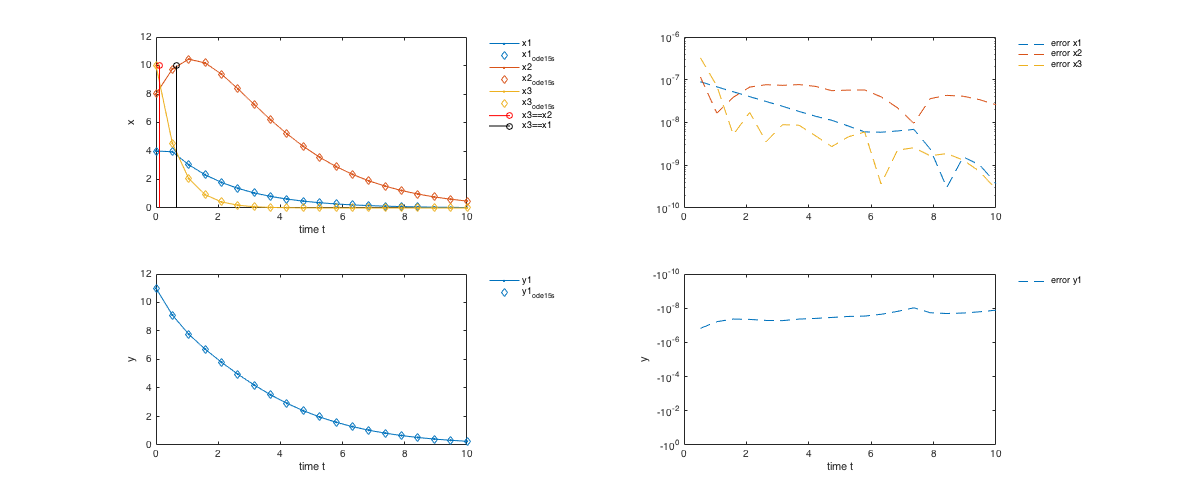
\includegraphics[width=\textwidth]{../../examples/example_1/html/example_model_1_01.png}
\begin{par}
FORWARD SENSITIVITY ANALYSIS
\end{par} \vspace{1em}
\begin{DoxyCode}
options.sensi = 1;

sol = simulate_model_example_1(t,log10(p),k,[],options);
\end{DoxyCode}
\begin{par}
FINITE DIFFERENCES
\end{par} \vspace{1em}
\begin{DoxyCode}
eps = 1e-4;
xi = log10(p);
for ip = 1:4;
    xip = xi;
    xip(ip) = xip(ip) + eps;
    solp = simulate_model_example_1(t,xip,k,[],options);
    sx_fd(:,:,ip) = (solp.x - sol.x)/eps;
    sy_fd(:,:,ip) = (solp.y - sol.y)/eps;
    sroot_fd(:,:,ip) = (solp.root - sol.root)/eps;
end
\end{DoxyCode}
\begin{par}
PLOTTING
\end{par} \vspace{1em}
\begin{DoxyCode}
figure
for ip = 1:4
    subplot(4,2,ip*2-1)
    hold on
    for ix = 1:size(sol.x,2)
        plot(t,sol.sx(:,ix,ip),'.-','Color',c_x(ix,:))
        plot(t,sx_fd(:,ix,ip),'d','Color',c_x(ix,:))
    end
    legend('x1','x1_{fd}','x2','x2_{fd}','x3','x3_{fd}','Location','NorthEastOutside')
    legend boxoff
    title(['state sensitivity for p' num2str(ip)])
    xlabel('time t')
    ylabel('x')
    box on

    subplot(4,2,ip*2)
    plot(t,abs(sol.sx(:,:,ip)-sx_fd(:,:,ip)),'--')
    legend('error x1','error x2','error x3','Location','NorthEastOutside')
    legend boxoff
    title(['state sensitivity for p' num2str(ip)])
    xlabel('time t')
    ylabel('error')
    set(gca,'YScale','log')
    box on
end
set(gcf,'Position',[100 300 1200 500])

figure
for ip = 1:4
    subplot(4,2,ip*2-1)
    hold on
    for iy = 1:size(sol.y,2)
        plot(t,sol.sy(:,iy,ip),'.-','Color',c_x(iy,:))
        plot(t,sy_fd(:,iy,ip),'d','Color',c_x(iy,:))
    end
    legend('y1','y1_fd','Location','NorthEastOutside')
    legend boxoff
    title(['observable sensitivity for p' num2str(ip)])
    xlabel('time t')
    ylabel('y')
    box on

    subplot(4,2,ip*2)
    plot(t,abs(sol.sy(:,:,ip)-sy_fd(:,:,ip)),'--')
    legend('error y1','Location','NorthEastOutside')
    legend boxoff
    title(['error observable sensitivity for p' num2str(ip)])
    xlabel('time t')
    ylabel('error')
    set(gca,'YScale','log')
    box on
end
set(gcf,'Position',[100 300 1200 500])

figure
for ip = 1:4
subplot(4,2,2*ip-1)
bar(1:6,sol.sroot(1:6,:,ip),0.8)
hold on
bar(1:6,sroot_fd(1:6,:,ip),0.4)
legend('x3==x2','x3==x1','x3==x2 fd','x3==x1 fd','Location','NorthEastOutside')
legend boxoff
title(['event sensitivity for p' num2str(ip)])
xlabel('event #')
ylabel('y')
box on

subplot(4,2,2*ip)
bar(1:6,sol.sroot(1:6,:,ip)-sroot_fd(1:6,:,ip),0.8)
legend('error x3==x2','error x3==x1','Location','NorthEastOutside')
legend boxoff
title(['error event sensitivity for p' num2str(ip)])
xlabel('event #')
ylabel('y')
box on
end
set(gcf,'Position',[100 300 1200 500])
\end{DoxyCode}

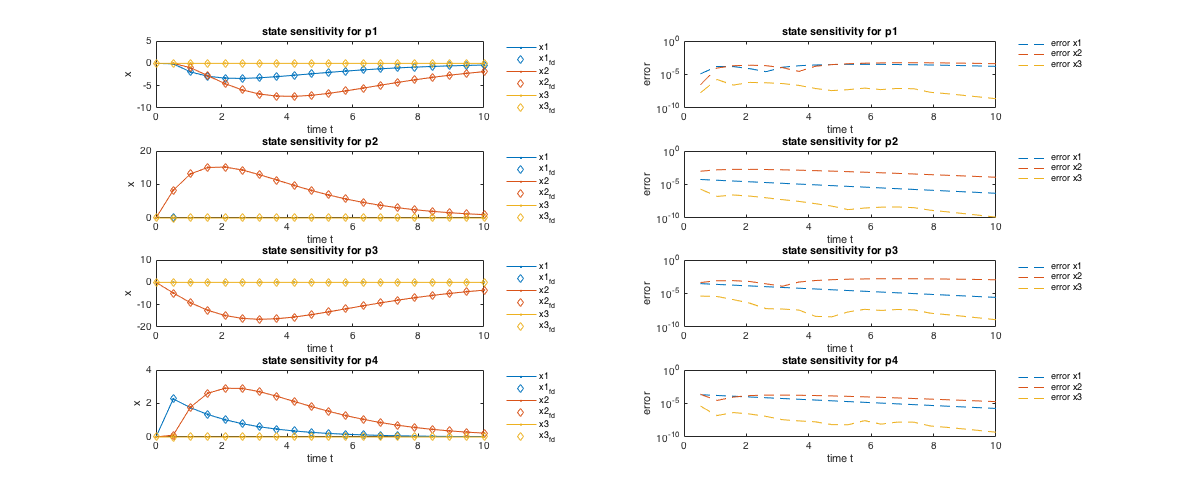
\includegraphics[width=\textwidth]{../../examples/example_1/html/example_model_1_02.png}

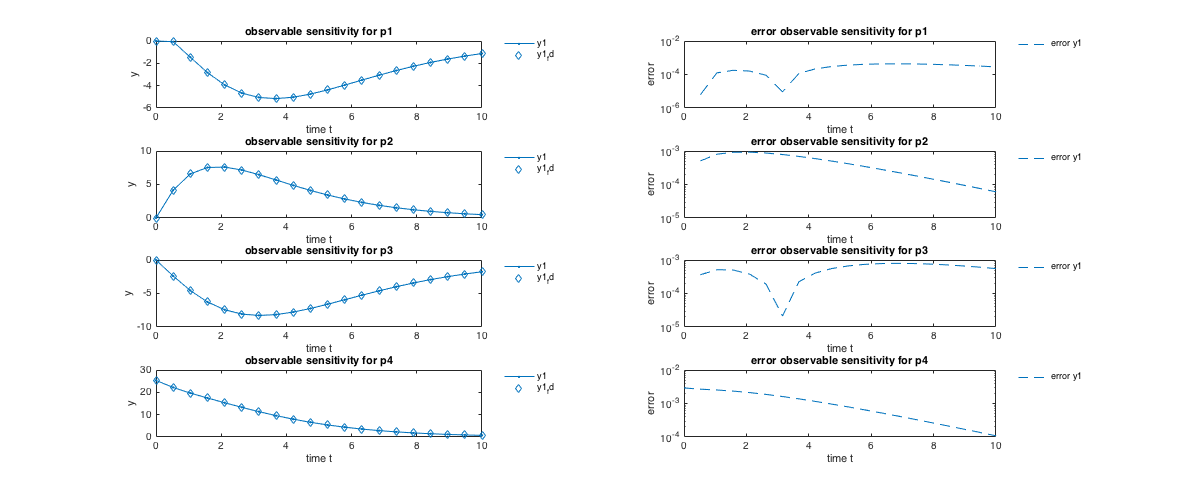
\includegraphics[width=\textwidth]{../../examples/example_1/html/example_model_1_03.png}

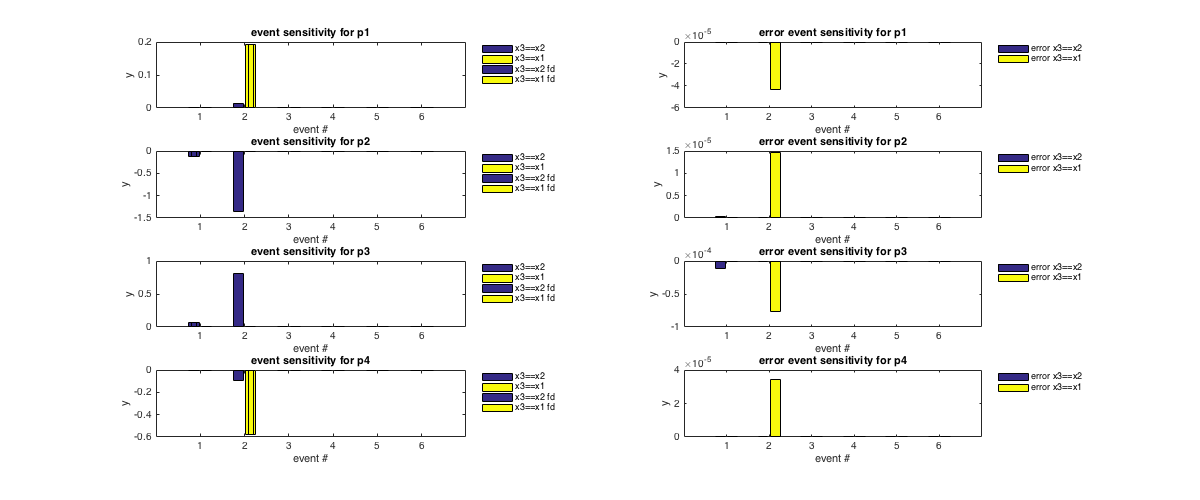
\includegraphics[width=\textwidth]{../../examples/example_1/html/example_model_1_04.png}




     \hypertarget{example2}{}\subsection{Example 2}\label{example2}
\hypertarget{example2_def2}{}\subsubsection{Model Definition}\label{example2_def2}
 
% This LaTeX was auto-generated from MATLAB code.
% To make changes, update the MATLAB code and republish this document.











    
    \begin{DoxyCode}
function [model] = example_model_2_syms()
\end{DoxyCode}
\begin{par}
CVODES OPTIONS
\end{par} \vspace{1em}
\begin{DoxyCode}
% set the default absolute tolerance
model.atol = 1e-8;
% set the default relative tolerance
model.rtol = 1e-8;
% set the default maximum number of integration steps
model.maxsteps = 1e4;
% set the parametrisation of the problem options are 'log', 'log10' and
% 'lin' (default).
model.param = 'log10';
\end{DoxyCode}
\begin{par}
STATES
\end{par} \vspace{1em}
\begin{DoxyCode}
% create state syms
syms x1 x2

% create state vector
x = [ x1 x2 ];
\end{DoxyCode}
\begin{par}
PARAMETERS ( for these sensitivities will be computed )
\end{par} \vspace{1em}
\begin{DoxyCode}
% create parameter syms
syms p1 p2 p3 p4

% create parameter vector
p = [p1,p2,p3,p4];
\end{DoxyCode}
\begin{par}
SYSTEM EQUATIONS
\end{par} \vspace{1em}
\begin{DoxyCode}
% create symbolic variable for time
syms t

xdot = sym(zeros(size(x)));

% piecewise defined function
xdot(1) = -p1*x1 + dirac(t-p2);
% inhomogeneous
xdot(2) = p3*x1 - p4*x2 ;
\end{DoxyCode}
\begin{par}
INITIAL CONDITIONS
\end{par} \vspace{1em}
\begin{DoxyCode}
x0 = sym(zeros(size(x)));

x0(1) = 0;
x0(2) = 0;
\end{DoxyCode}
\begin{par}
OBSERVALES
\end{par} \vspace{1em}
\begin{DoxyCode}
y = sym(zeros(1,1));

y(1) = x2;
\end{DoxyCode}
\begin{par}
SYSTEM STRUCT
\end{par} \vspace{1em}
\begin{DoxyCode}
model.sym.x = x;
model.sym.xdot = xdot;
model.sym.p = p;
model.sym.x0 = x0;
model.sym.y = y;
\end{DoxyCode}
\begin{DoxyCode}
end
\end{DoxyCode}

         \begin{DoxyCode}ans = 
        atol: 1e-08
        rtol: 1e-08
    maxsteps: 10000
       param: 'log10'
         sym: [1x1 struct]
\end{DoxyCode} 
    



    \hypertarget{example2_simu2}{}\subsubsection{Simulation}\label{example2_simu2}
 
% This LaTeX was auto-generated from MATLAB code.
% To make changes, update the MATLAB code and republish this document.











    
    \begin{DoxyCode}
clear
\end{DoxyCode}
\begin{par}
COMPILATION
\end{par} \vspace{1em}
\begin{DoxyCode}
[exdir,~,~]=fileparts(which('example_model_2.m'));
% compile the model
amiwrap('model_example_2','example_model_2_syms',exdir)
\end{DoxyCode}

         \begin{DoxyCode}Generating model struct ...
Parsing model struct ...
Generating C code ...
headers | wrapfunctions | 
Compiling mex file ...
Building with 'Xcode with Clang'.
MEX completed successfully.
\end{DoxyCode} 
    \begin{par}
SIMULATION
\end{par} \vspace{1em}
\begin{DoxyCode}
% time vector
t = linspace(0,3,1001);
p = [1;0.5;2;3];
k = [];

options.sensi = 0;
options.cvode_maxsteps = 1e6;
% load mex into memory
[msg] = which('simulate_model_example_2'); % fix for inaccessability problems
sol = simulate_model_example_2(t,log10(p),k,[],options);

tic
sol = simulate_model_example_2(t,log10(p),k,[],options);
disp(['Time elapsed with amiwrap: ' num2str(toc) ])
\end{DoxyCode}

         \begin{DoxyCode}Time elapsed with amiwrap: 0.0019205
\end{DoxyCode} 
    \begin{par}
ODE15S
\end{par} \vspace{1em}
\begin{DoxyCode}
sig = 1e-2;
delta_num = @(tau) exp(-1/2*(tau/sig).^2)/(sqrt(2*pi)*sig);

ode_system = @(t,x,p,k) [-p(1)*x(1)+delta_num(t-p(2));
    +p(3)*x(1) - p(4)*x(2)];

options_ode45 = odeset('RelTol',1e-8,'AbsTol',1e-8,'MaxStep',1e4);

tic
[~, X_ode45] = ode45(@(t,x) ode_system(t,x,p,k),t,[0;0],options_ode45);
disp(['Time elapsed with ode45: ' num2str(toc) ])
\end{DoxyCode}

         \begin{DoxyCode}Time elapsed with ode45: 0.042852
\end{DoxyCode} 
    \begin{par}
PLOTTING
\end{par} \vspace{1em}
\begin{DoxyCode}
figure
c_x = get(gca,'ColorOrder');
subplot(2,2,1)
for ix = 1:size(sol.x,2)
    plot(t,sol.x(:,ix),'.-','Color',c_x(ix,:))
    hold on
    plot(t,X_ode45(:,ix),'--','Color',c_x(ix,:))
end

legend('x1','x1_{ode45}','x2','x2_{ode15s}','Location','NorthEastOutside')
legend boxoff
xlabel('time t')
ylabel('x')
box on
subplot(2,2,2)
plot(t,abs(sol.x-X_ode45),'--')
set(gca,'YScale','log')
ylim([1e-10,1e0])
legend('error x1','error x2','Location','NorthEastOutside')
legend boxoff

subplot(2,2,3)
plot(t,sol.y,'.-','Color',c_x(1,:))
hold on
plot(t,X_ode45(:,2),'--','Color',c_x(1,:))
legend('y1','y1_{ode45}','Location','NorthEastOutside')
legend boxoff
xlabel('time t')
ylabel('y')
box on

subplot(2,2,4)
plot(t,abs(sol.y-X_ode45(:,2)),'--')
set(gca,'YScale','log')
ylim([1e-10,1e0])
legend('error y1','Location','NorthEastOutside')
legend boxoff
xlabel('time t')
ylabel('y')
box on
set(gcf,'Position',[100 300 1200 500])
\end{DoxyCode}

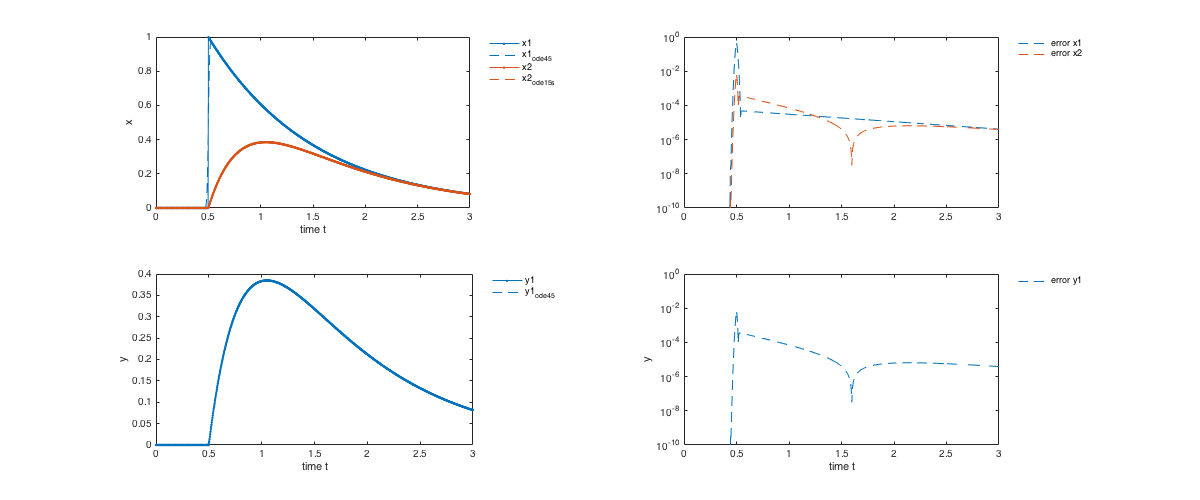
\includegraphics [width=4in]{../../examples/example_2/html/example_model_2_01.png}
\begin{par}
FORWARD SENSITIVITY ANALYSIS
\end{par} \vspace{1em}
\begin{DoxyCode}
options.sensi = 1;

sol = simulate_model_example_2(t,log10(p),k,[],options);
\end{DoxyCode}
\begin{par}
FINITE DIFFERENCES
\end{par} \vspace{1em}
\begin{DoxyCode}
eps = 1e-4;
xi = log10(p);
for ip = 1:4;
    xip = xi;
    xip(ip) = xip(ip) + eps;
    solp = simulate_model_example_2(t,xip,k,[],options);
    sx_fd(:,:,ip) = (solp.x - sol.x)/eps;
    sy_fd(:,:,ip) = (solp.y - sol.y)/eps;
end
\end{DoxyCode}
\begin{par}
PLOTTING
\end{par} \vspace{1em}
\begin{DoxyCode}
figure
for ip = 1:4
    subplot(4,2,ip*2-1)
    hold on
    for ix = 1:size(sol.x,2)
        plot(t,sol.sx(:,ix,ip),'.-','Color',c_x(ix,:))
        plot(t,sx_fd(:,ix,ip),'--','Color',c_x(ix,:))
    end
    ylim([-2,2])
    legend('x1','x1_{fd}','x2','x2_{fd}','Location','NorthEastOutside')
    legend boxoff
    title(['state sensitivity for p' num2str(ip)])
    xlabel('time t')
    ylabel('x')
    box on

    subplot(4,2,ip*2)
    plot(t,abs(sol.sx(:,:,ip)-sx_fd(:,:,ip)),'r--')
    legend('error x1','error x2','Location','NorthEastOutside')
    legend boxoff
    title(['state sensitivity for p' num2str(ip)])
    xlabel('time t')
    ylabel('error')
    ylim([1e-12,1e0])
    set(gca,'YScale','log')
    box on
end
set(gcf,'Position',[100 300 1200 500])

figure
for ip = 1:4
    subplot(4,2,ip*2-1)
    hold on
    for iy = 1:size(sol.y,2)
        plot(t,sol.sy(:,iy,ip),'.-','Color',c_x(iy,:))
        plot(t,sy_fd(:,iy,ip),'--','Color',c_x(iy,:))
    end
    ylim([-2,2])
    legend('y1','y1_{fd}','Location','NorthEastOutside')
    legend boxoff
    title(['observable sensitivity for p' num2str(ip)])
    xlabel('time t')
    ylabel('y')
    box on

    subplot(4,2,ip*2)
    plot(t,abs(sol.sy(:,:,ip)-sy_fd(:,:,ip)),'r--')
    legend('error y1','Location','NorthEastOutside')
    legend boxoff
    title(['observable sensitivity for p' num2str(ip)])
    xlabel('time t')
    ylabel('error')
    ylim([1e-12,1e0])
    set(gca,'YScale','log')
    box on
end
set(gcf,'Position',[100 300 1200 500])
\end{DoxyCode}

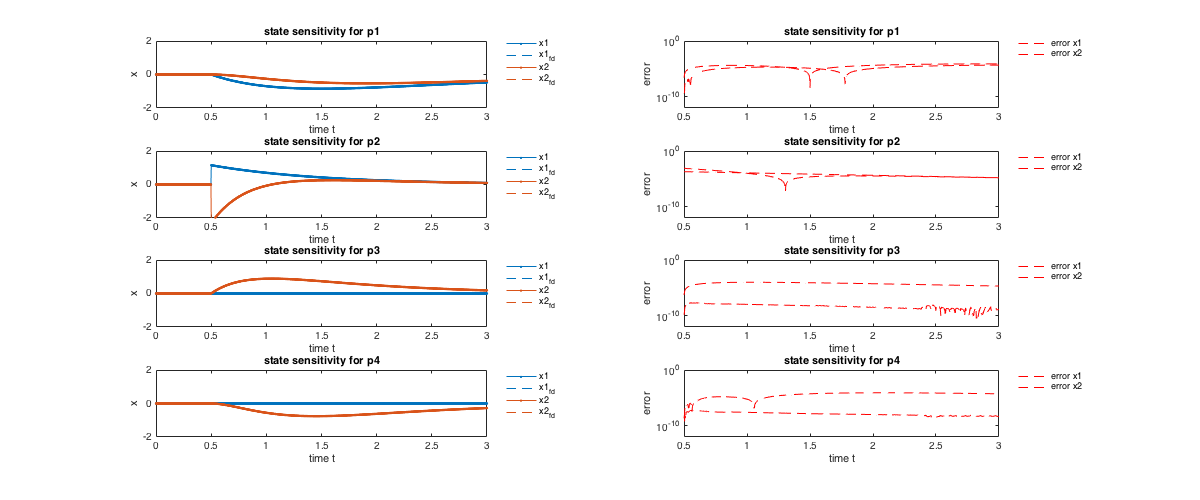
\includegraphics [width=4in]{../../examples/example_2/html/example_model_2_02.png}

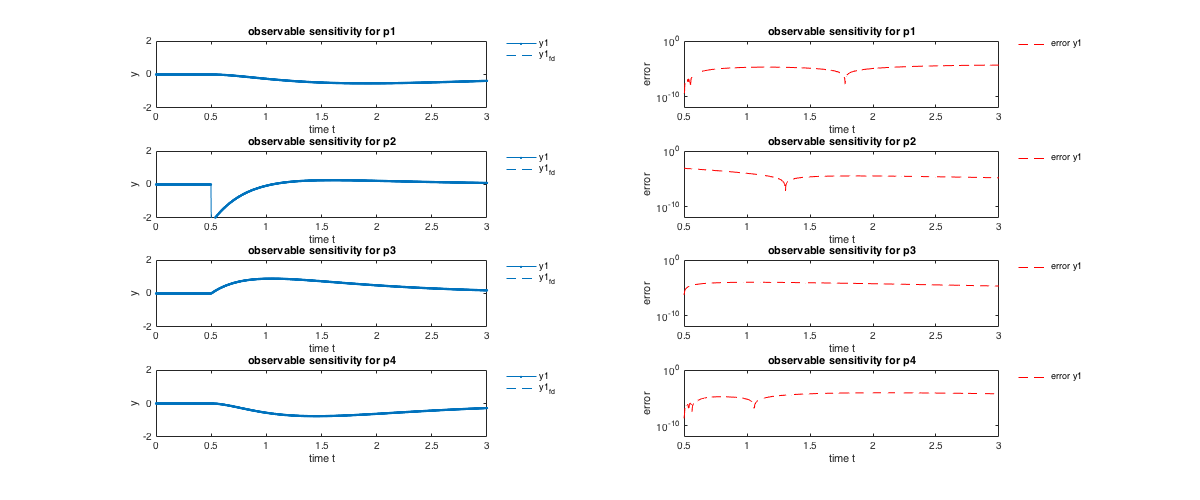
\includegraphics [width=4in]{../../examples/example_2/html/example_model_2_03.png}




     \hypertarget{example3}{}\subsection{Example 3}\label{example3}
\hypertarget{example3_def3}{}\subsubsection{Model Definition}\label{example3_def3}
 
% This LaTeX was auto-generated from MATLAB code.
% To make changes, update the MATLAB code and republish this document.











    
    \begin{DoxyCode}
function [model] = example_model_3_syms()
\end{DoxyCode}
\begin{par}
CVODES OPTIONS
\end{par} \vspace{1em}
\begin{DoxyCode}
% set the default absolute tolerance
model.atol = 1e-8;
% set the default relative tolerance
model.rtol = 1e-8;
% set the default maximum number of integration steps
model.maxsteps = 1e4;
% set the parametrisation of the problem options are 'log', 'log10' and
% 'lin' (default).
model.param = 'log10';
\end{DoxyCode}
\begin{par}
STATES
\end{par} \vspace{1em}
\begin{DoxyCode}
% create state syms
syms x1 x2 x3

% create state vector
x = [
x1 x2 x3
];
\end{DoxyCode}
\begin{par}
PARAMETERS ( for these sensitivities will be computed )
\end{par} \vspace{1em}
\begin{DoxyCode}
% create parameter syms
syms p1 p2 p3 p4 p5

% create parameter vector
p = [p1,p2,p3,p4,p5];
\end{DoxyCode}
\begin{par}
CONSTANTS ( for these no sensitivities will be computed ) this part is optional and can be ommited
\end{par} \vspace{1em}
\begin{DoxyCode}
% create parameter syms
syms k1 k2 k3 k4

% create parameter vector
k = [k1 k2 k3 k4];
\end{DoxyCode}
\begin{par}
SYSTEM EQUATIONS
\end{par} \vspace{1em}
\begin{DoxyCode}
% create symbolic variable for time
syms t

xdot = sym(zeros(size(x)));

% piecewise defined function
xdot(1) = -2*p1*x1^2 - p2*x1*x2 + 2*p3*x2 + p4*x3 + p5;
% inhomogeneous
xdot(2) = +p1*x1^2 - p2*x1*x2 - p3*x2 + p4*x3;
xdot(3) = p2*x1*x2 - p4*x(3) - k4*x(3);
\end{DoxyCode}
\begin{par}
INITIAL CONDITIONS
\end{par} \vspace{1em}
\begin{DoxyCode}
x0 = sym(zeros(size(x)));

x0(1) = k1;
x0(2) = k2;
x0(3) = k3;
\end{DoxyCode}
\begin{par}
OBSERVALES
\end{par} \vspace{1em}
\begin{DoxyCode}
y = sym(zeros(1,1));

y = x;
\end{DoxyCode}
\begin{par}
SYSTEM STRUCT
\end{par} \vspace{1em}
\begin{DoxyCode}
model.sym.x = x;
model.sym.k = k;
model.sym.xdot = xdot;
model.sym.p = p;
model.sym.x0 = x0;
model.sym.y = y;
\end{DoxyCode}
\begin{DoxyCode}
end
\end{DoxyCode}

         \begin{DoxyCode}ans = 
        atol: 1e-08
        rtol: 1e-08
    maxsteps: 10000
       param: 'log10'
         sym: [1x1 struct]
\end{DoxyCode} 
    



    \hypertarget{example3_simu3}{}\subsubsection{Simulation}\label{example3_simu3}
 
% This LaTeX was auto-generated from MATLAB code.
% To make changes, update the MATLAB code and republish this document.











    
    \begin{DoxyCode}
clear
\end{DoxyCode}
\begin{par}
COMPILATION
\end{par} \vspace{1em}
\begin{DoxyCode}
[exdir,~,~]=fileparts(which('example_model_3.m'));
% compile the model
amiwrap('model_example_3','example_model_3_syms',exdir)
% add the model to the path
addpath(genpath([strrep(which('amiwrap.m'),'amiwrap.m','') 'models/model_example_3']))
\end{DoxyCode}

         \begin{DoxyCode}Generating model struct ...
Parsing model struct ...
Generating C code ...
headers | wrapfunctions | 
Compiling mex file ...
Building with 'Xcode with Clang'.
MEX completed successfully.
\end{DoxyCode} 
    \begin{par}
SIMULATION
\end{par} \vspace{1em}
\begin{DoxyCode}
% time vector
t = linspace(0,300,20);
p = [1;0.5;0.4;2;0.1];
k = [0.1,0.4,0.7,1];

options.sensi = 0;
options.cvode_maxsteps = 1e6;
% load mex into memory
sol = simulate_model_example_3(t,log10(p),k,[],options);

tic
sol = simulate_model_example_3(t,log10(p),k,[],options);
disp(['Time elapsed with cvodes: ' num2str(toc) ])
\end{DoxyCode}

         \begin{DoxyCode}Time elapsed with cvodes: 0.002146
\end{DoxyCode} 
    \begin{par}
ODE15S
\end{par} \vspace{1em}
\begin{DoxyCode}
ode_system = @(t,x,p,k) [-2*p(1)*x(1)^2 - p(2)*x(1)*x(2) + 2*p(3)*x(2) + p(4)*x(3) + p(5);
    + p(1)*x(1)^2 - p(2)*x(1)*x(2) - p(3)*x(2) + p(4)*x(3);
    + p(2)*x(1)*x(2) - p(4)*x(3) - k(4)*x(3)];
options_ode15s = odeset('RelTol',1e-8,'AbsTol',1e-8,'MaxStep',1e4);

tic
[~, X_ode15s] = ode15s(@(t,x) ode_system(t,x,p,k),t,k(1:3),options_ode15s);
disp(['Time elapsed with ode15s: ' num2str(toc) ])
\end{DoxyCode}

         \begin{DoxyCode}Time elapsed with ode15s: 0.18018
\end{DoxyCode} 
    \begin{par}
PLOTTING
\end{par} \vspace{1em}
\begin{DoxyCode}
figure
c_x = get(gca,'ColorOrder');
subplot(2,2,1)
for ix = 1:size(sol.x,2)
    plot(t,sol.x(:,ix),'.-','Color',c_x(ix,:))
    hold on
    plot(t,X_ode15s(:,ix),'d','Color',c_x(ix,:))
end
legend('x1','x1_{ode15s}','x2','x2_{ode15s}','x3','x3_{ode15s}','Location','NorthEastOutside')
legend boxoff
xlabel('time t')
ylabel('x')
box on
subplot(2,2,2)
plot(t,abs(sol.x-X_ode15s),'--')
set(gca,'YScale','log')
legend('error x1','error x2','error x3','Location','NorthEastOutside')
legend boxoff
set(gcf,'Position',[100 300 1200 500])
\end{DoxyCode}

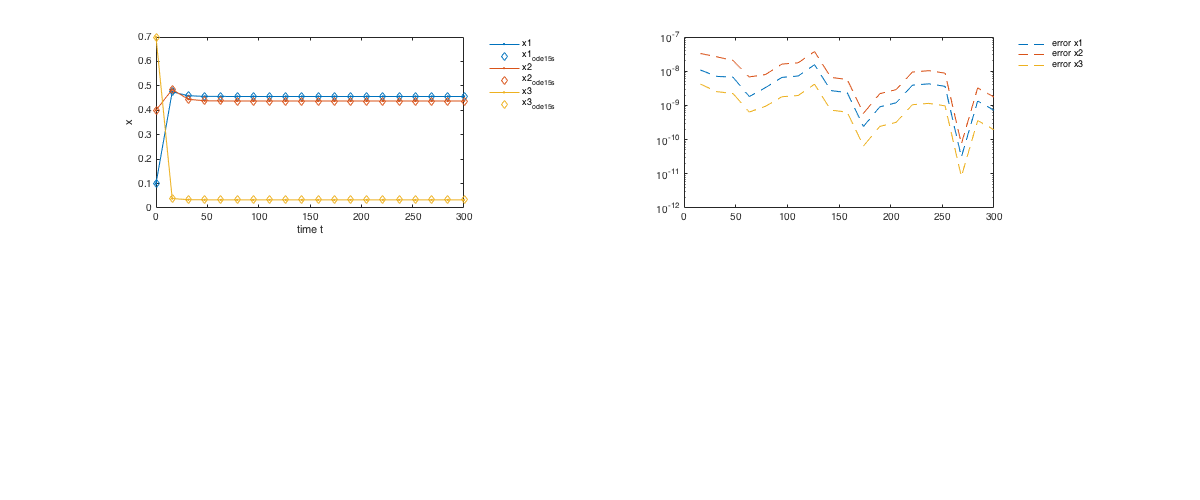
\includegraphics [width=4in]{../../examples/example_3/html/example_model_3_01.png}
\begin{par}
FORWARD SENSITIVITY ANALYSIS
\end{par} \vspace{1em}
\begin{DoxyCode}
options.sensi = 1;
options.sens_ind = [3,1,2,4];

sol = simulate_model_example_3(t,log10(p),k,[],options);
\end{DoxyCode}
\begin{par}
FINITE DIFFERENCES
\end{par} \vspace{1em}
\begin{DoxyCode}
eps = 1e-3;

xi = log10(p);
for ip = 1:4;
    xip = xi;
    xip(ip) = xip(ip) + eps;
    solp = simulate_model_example_3(t,xip,k,[],options);
    sx_fd(:,:,ip) = (solp.x - sol.x)/eps;
    sy_fd(:,:,ip) = (solp.y - sol.y)/eps;
end
\end{DoxyCode}
\begin{par}
PLOTTING
\end{par} \vspace{1em}
\begin{DoxyCode}
figure
for ip = 1:4
    subplot(4,2,ip*2-1)
    hold on
    for ix = 1:size(sol.x,2)
        plot(t,sol.sx(:,ix,ip),'.-','Color',c_x(ix,:))
        plot(t,sx_fd(:,ix,options.sens_ind(ip)),'d','Color',c_x(ix,:))
    end
    legend('x1','x1_{fd}','x2','x2_{fd}','x3','x3_{fd}','Location','NorthEastOutside')
    legend boxoff
    title(['state sensitivity for p' num2str(options.sens_ind(ip))])
    xlabel('time t')
    ylabel('x')
    box on

    subplot(4,2,ip*2)
    plot(t,abs(sol.sx(:,:,ip)-sx_fd(:,:,options.sens_ind(ip))),'--')
    legend('error x1','error x2','error x3','Location','NorthEastOutside')
    legend boxoff
    title(['error of state sensitivity for p' num2str(options.sens_ind(ip))])
    xlabel('time t')
    ylabel('error')
    set(gca,'YScale','log')
    box on
end
set(gcf,'Position',[100 300 1200 500])
\end{DoxyCode}

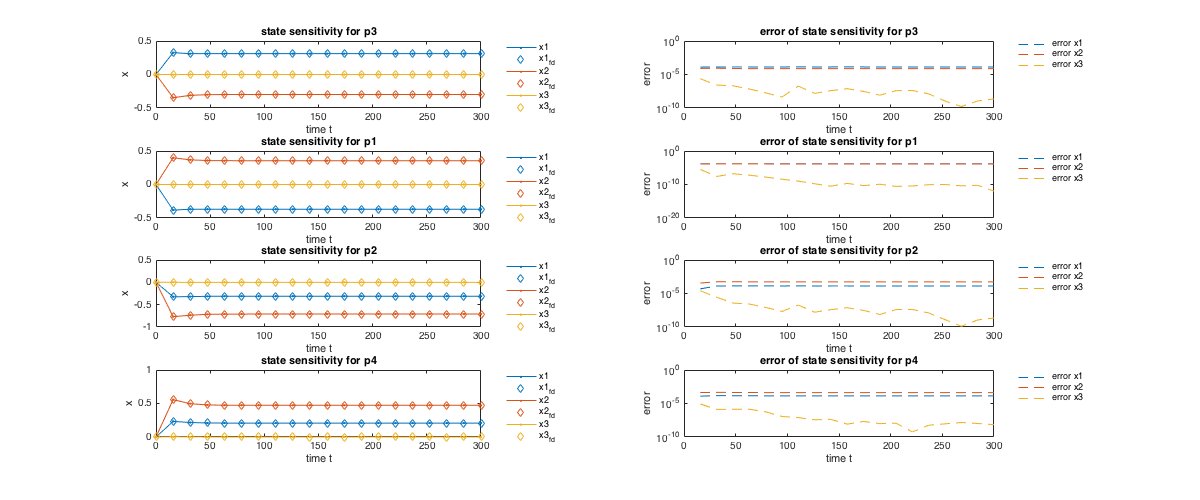
\includegraphics [width=4in]{../../examples/example_3/html/example_model_3_02.png}
\begin{par}
STEADY STATE SENSITIVITY
\end{par} \vspace{1em}
\begin{DoxyCode}
sssens = NaN(size(sol.sx));
for it = 2:length(t)
    tt = [0,t(it)];
    options.sensi_meth = 'ss';
    solss = simulate_model_example_3(tt,log10(p),k,[],options);
    sssens(it,:,:) = solss.sx;
    ssxdot(it,:) = solss.xdot;
end
\end{DoxyCode}
\begin{par}
PLOTTING
\end{par} \vspace{1em}
\begin{DoxyCode}
figure
for ip = 1:4
    subplot(4,2,ip*2-1)
    hold on
    for ix = 1:size(sol.x,2)
        plot(t,sol.sx(:,ix,ip),'.-','Color',c_x(ix,:))
        plot(t,sssens(:,ix,ip),'d-','Color',c_x(ix,:))
    end
    legend('x1','x1_{ss}','x2','x2_{ss}','x3','x3_{ss}','Location','NorthEastOutside')
    legend boxoff
    title(['state steady sensitivity for p' num2str(ip)])
    xlabel('time t')
    ylabel('x')
    box on

    subplot(4,2,ip*2)
    plot(t,abs(sol.sx(:,:,ip)-sssens(:,:,ip)),'--')
    legend('error x1','error x2','error x3','Location','NorthEastOutside')
    legend boxoff
    title(['error of steady state sensitivity for p' num2str(ip)])
    xlabel('time t')
    ylabel('error')
    set(gca,'YScale','log')
    box on
end
set(gcf,'Position',[100 300 1200 500])

figure
scatter(sqrt(sum((ssxdot./sol.x).^2,2)),sqrt(sum(sum((sol.sx-sssens).^2,2),3)))
hold on
plot([1e-15,1e5],[1e-15,1e5],'k:')
set(gca,'YScale','log')
set(gca,'XScale','log')
box on
axis square
xlabel('||dxdt/x||_2')
ylabel('error steady state approximation')
set(gca,'FontSize',15)
set(gca,'LineWidth',1.5)
set(gcf,'Position',[100 300 1200 500])
\end{DoxyCode}

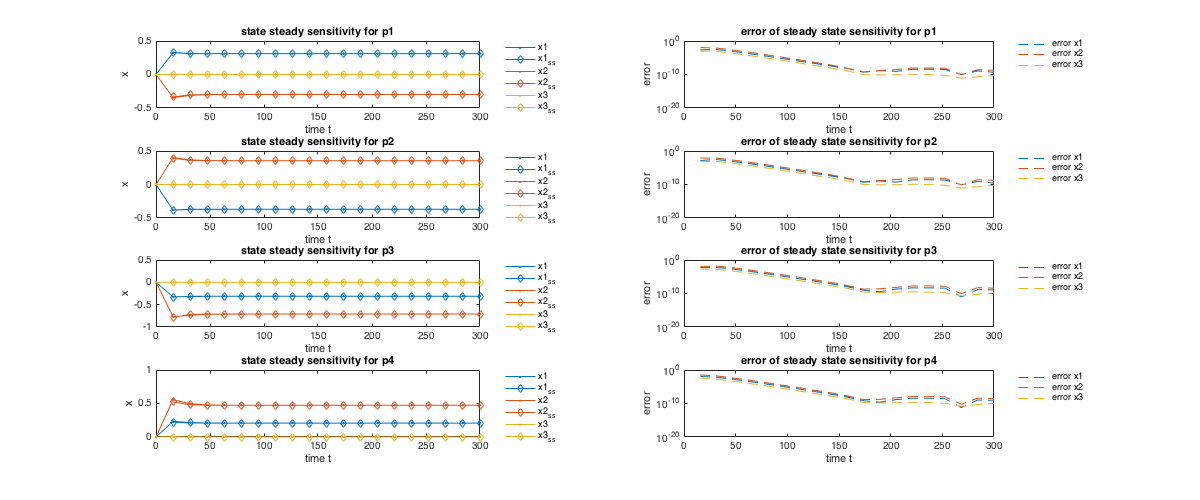
\includegraphics [width=4in]{../../examples/example_3/html/example_model_3_03.png}

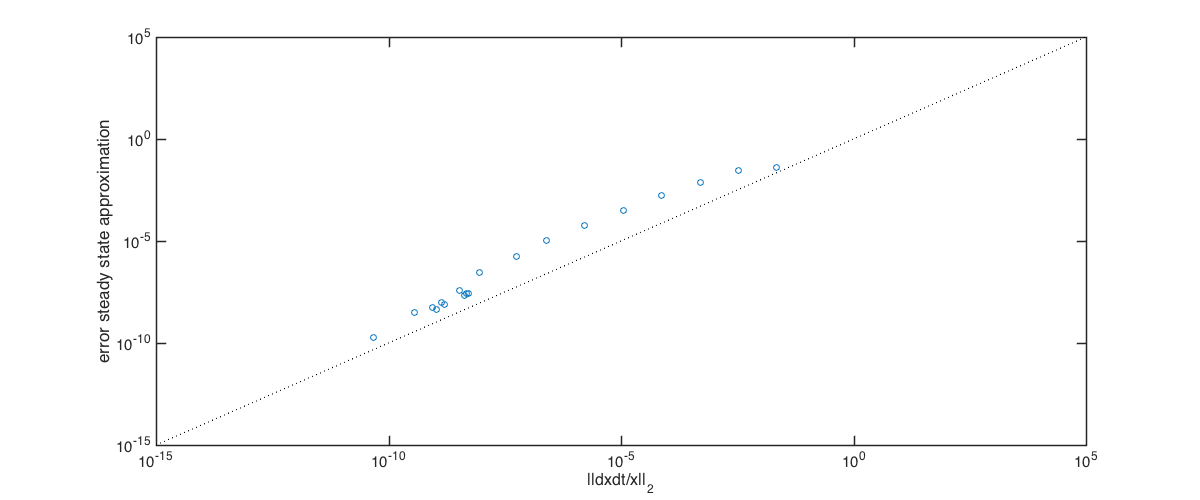
\includegraphics [width=4in]{../../examples/example_3/html/example_model_3_04.png}




     \hypertarget{example4}{}\subsection{Example 4}\label{example4}
\hypertarget{example4_def4}{}\subsubsection{Model Definition}\label{example4_def4}
 
% This LaTeX was auto-generated from MATLAB code.
% To make changes, update the MATLAB code and republish this document.











    
    \begin{DoxyCode}
function [model] = example_model_4_syms()
\end{DoxyCode}
\begin{par}
CVODES OPTIONS
\end{par} \vspace{1em}
\begin{DoxyCode}
model.atol = 1e-12;
model.rtol = 1e-8;
model.maxsteps = 1e4;
model.param = 'log10';
\end{DoxyCode}
\begin{par}
STATES
\end{par} \vspace{1em}
\begin{DoxyCode}
syms STAT pSTAT pSTAT_pSTAT npSTAT_npSTAT nSTAT1 nSTAT2 nSTAT3 nSTAT4 nSTAT5

x = [
STAT, pSTAT, pSTAT_pSTAT, npSTAT_npSTAT, nSTAT1, nSTAT2, nSTAT3, nSTAT4, nSTAT5 ...
];
\end{DoxyCode}
\begin{par}
PARAMETERS
\end{par} \vspace{1em}
\begin{DoxyCode}
syms p1 p2 p3 p4 init_STAT Omega_cyt Omega_nuc sp1 sp2 sp3 sp4 sp5 offset_tSTAT offset_pSTAT scale_tSTAT scale_pSTAT sigma_pSTAT sigma_tSTAT sigma_pEpoR

p = [p1,p2,p3,p4,init_STAT,sp1,sp2,sp3,sp4,sp5,offset_tSTAT,offset_pSTAT,scale_tSTAT,scale_pSTAT,sigma_pSTAT,sigma_tSTAT,sigma_pEpoR];

k = [Omega_cyt,Omega_nuc];
\end{DoxyCode}
\begin{par}
INPUT
\end{par} \vspace{1em}
\begin{DoxyCode}
syms t
u(1) = spline_pos5(t, 0.0, sp1, 5.0, sp2, 10.0, sp3, 20.0, sp4, 60.0, sp5, 0, 0.0);
\end{DoxyCode}
\begin{par}
SYSTEM EQUATIONS
\end{par} \vspace{1em}
\begin{DoxyCode}
xdot = sym(zeros(size(x)));

xdot(1) = (Omega_nuc*p4*nSTAT5 - Omega_cyt*STAT*p1*u(1))/Omega_cyt;
xdot(2) = STAT*p1*u(1) - 2*p2*pSTAT^2;
xdot(3) = p2*pSTAT^2 - p3*pSTAT_pSTAT;
xdot(4) = -(Omega_nuc*p4*npSTAT_npSTAT - Omega_cyt*p3*pSTAT_pSTAT)/Omega_nuc;
xdot(5) = -p4*(nSTAT1 - 2*npSTAT_npSTAT);
xdot(6) = p4*(nSTAT1 - nSTAT2);
xdot(7) = p4*(nSTAT2 - nSTAT3);
xdot(8) = p4*(nSTAT3 - nSTAT4);
xdot(9) = p4*(nSTAT4 - nSTAT5);
\end{DoxyCode}
\begin{par}
INITIAL CONDITIONS
\end{par} \vspace{1em}
\begin{DoxyCode}
x0 = sym(zeros(size(x)));

x0(1) = init_STAT;
\end{DoxyCode}
\begin{par}
OBSERVABLES
\end{par} \vspace{1em}
\begin{DoxyCode}
y = sym(zeros(3,1));

y(1) = offset_pSTAT + scale_pSTAT/init_STAT*(pSTAT + 2*pSTAT_pSTAT);
y(2) = offset_tSTAT + scale_tSTAT/init_STAT*(STAT + pSTAT + 2*(pSTAT_pSTAT));
y(3) = u(1);
\end{DoxyCode}
\begin{par}
SIGMA
\end{par} \vspace{1em}
\begin{DoxyCode}
sigma_y = sym(size(y));

sigma_y(1) = sigma_pSTAT;
sigma_y(2) = sigma_tSTAT;
sigma_y(3) = sigma_pEpoR;
\end{DoxyCode}
\begin{par}
SYSTEM STRUCT
\end{par} \vspace{1em}
\begin{DoxyCode}
model.sym.x = x;
model.sym.u = u;
model.sym.xdot = xdot;
model.sym.p = p;
model.sym.k = k;
model.sym.x0 = x0;
model.sym.y = y;
model.sym.sigma_y = sigma_y;
\end{DoxyCode}
\begin{DoxyCode}
end
\end{DoxyCode}

         \begin{DoxyCode}ans = 
        atol: 1e-12
        rtol: 1e-08
    maxsteps: 10000
       param: 'log10'
         sym: [1x1 struct]
\end{DoxyCode} 
    



    \hypertarget{example4_simu4}{}\subsubsection{Simulation}\label{example4_simu4}
 
% This LaTeX was auto-generated from MATLAB code.
% To make changes, update the MATLAB code and republish this document.











    
    \begin{DoxyCode}
clear
% compile the model
[exdir,~,~]=fileparts(which('example_model_4.m'));
amiwrap('model_example_4','example_model_4_syms',exdir)

num = xlsread(fullfile(exdir,'pnas_data_original.xls'));

t = num(:,1);

D.Y = num(:,[2,4,6]);
D.Sigma_Y = NaN(size(D.Y));


kappa = [1.4,0.45];

xi =  [0.595102743982229
    2.99999999999997
    -0.948930681736172
    -0.00751433662124028
    0
    -2.78593598707493
    -0.256066441623149
    -0.07511250551843
    -0.411247187909784
    -4.99999999959546
    -0.735327875726678
    -0.64146041506584
    -0.107897525629158
    0.0272647740863191
    -0.5
    0
    -0.5];

options.sensi = 0;
sol = simulate_model_example_4(t,xi,kappa,D,options);

figure
for iy = 1:3
    subplot(2,2,iy)
    plot(t,D.Y(:,iy),'rx')
    hold on
    plot(t,sol.y(:,iy),'.-')
    xlim([0,60])
    xlabel('t')
    switch(iy)
        case 1
            ylabel('pStat')
        case 2
            ylabel('tStat')
        case 3
            ylabel('pEpoR')
    end
    ylim([0,1.2])
end
set(gcf,'Position',[100 300 1200 500])

% generate new
xi_rand = xi + 0.1;
options.sensi = 1;
options.sensi_meth = 'adjoint';
sol = simulate_model_example_4(t,xi_rand,kappa,D,options);

options.sensi = 0;
eps = 1e-4;
fd_grad = NaN(length(xi),1);
for ip = 1:length(xi)
    xip = xi_rand;
    xip(ip) = xip(ip) + eps;
    psol = simulate_model_example_4(t,xip,kappa,D,options);
    fd_grad(ip) = (psol.llh-sol.llh)/eps;
end

figure
scatter(abs(sol.sllh),abs(fd_grad))
set(gca,'XScale','log')
set(gca,'YScale','log')
xlim([1e-2,1e2])
ylim([1e-2,1e2])
box on
hold on
axis square
plot([1e-2,1e2],[1e-2,1e2],'k:')
xlabel('adjoint sensitivity absolute value of gradient element')
ylabel('finite difference absolute value of gradient element')
set(gcf,'Position',[100 300 1200 500])
\end{DoxyCode}

         \begin{DoxyCode}Generating model struct ...
Parsing model struct ...
Generating C code ...
headers | wrapfunctions | 
Compiling mex file ...
Building with 'Xcode with Clang'.
MEX completed successfully.
\end{DoxyCode} 
    
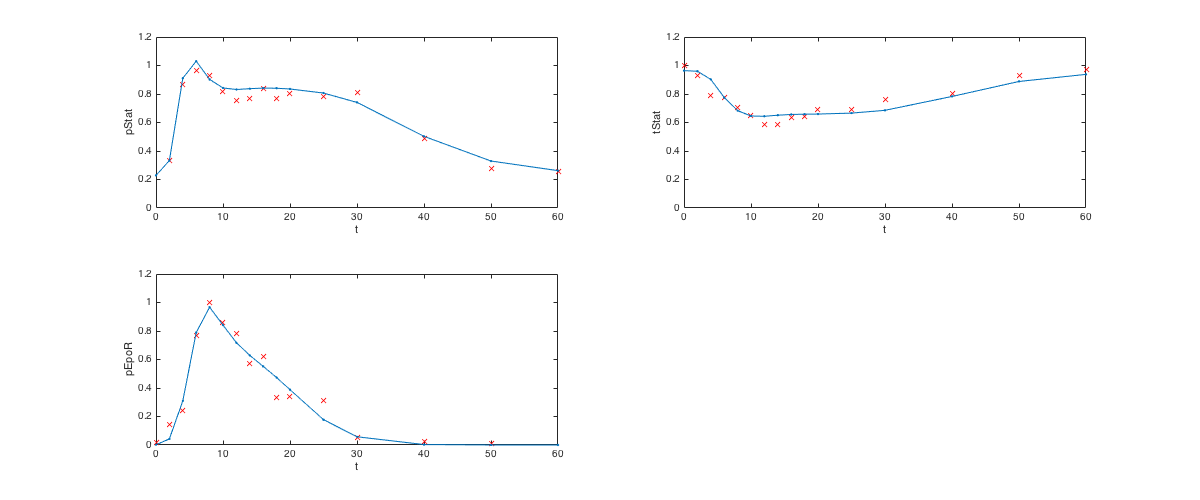
\includegraphics [width=4in]{../../examples/example_4/html/example_model_4_01.png}

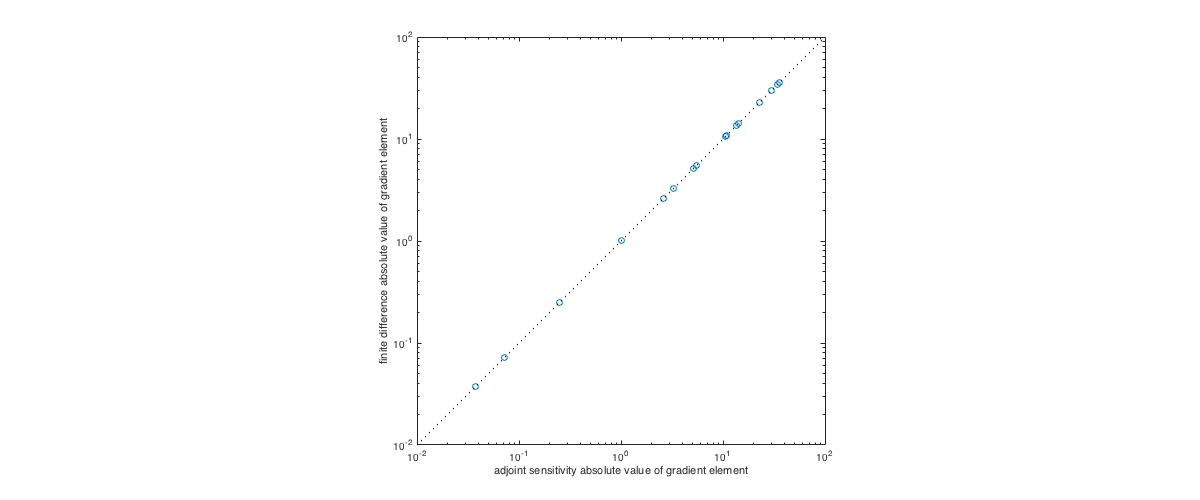
\includegraphics [width=4in]{../../examples/example_4/html/example_model_4_02.png}




     \hypertarget{example5}{}\subsection{Example 5}\label{example5}
\hypertarget{example5_def5}{}\subsubsection{Model Definition}\label{example5_def5}
 
% This LaTeX was auto-generated from MATLAB code.
% To make changes, update the MATLAB code and republish this document.











    
    \begin{DoxyCode}
function [model] = example_model_5_syms()
\end{DoxyCode}
\begin{par}
CVODES OPTIONS
\end{par} \vspace{1em}
\begin{DoxyCode}
% set the default absolute tolerance
model.atol = 1e-8;
% set the default relative tolerance
model.rtol = 1e-8;
% set the default maximum number of integration steps
model.maxsteps = 1e4;
% set the parametrisation of the problem options are 'log', 'log10' and
% 'lin' (default).
model.param = 'log10';
\end{DoxyCode}
\begin{par}
STATES
\end{par} \vspace{1em}
\begin{DoxyCode}
% create state syms
syms x1 x2

% create state vector
x = [ x1 x2 ];
\end{DoxyCode}
\begin{par}
PARAMETERS ( for these sensitivities will be computed )
\end{par} \vspace{1em}
\begin{DoxyCode}
% create parameter syms
syms p1 p2 p3 p4

% create parameter vector
p = [p1,p2,p3,p4];
\end{DoxyCode}
\begin{par}
SYSTEM EQUATIONS
\end{par} \vspace{1em}
\begin{DoxyCode}
% create symbolic variable for time
syms t

xdot = sym(zeros(size(x)));

% piecewise defined function
xdot(1) = -p1*x1 + dirac(t-p2);
% inhomogeneous
xdot(2) = p3*x1 - p4*x2 ;
\end{DoxyCode}
\begin{par}
INITIAL CONDITIONS
\end{par} \vspace{1em}
\begin{DoxyCode}
x0 = sym(zeros(size(x)));

x0(1) = 0;
x0(2) = 0;
\end{DoxyCode}
\begin{par}
OBSERVALES
\end{par} \vspace{1em}
\begin{DoxyCode}
y = sym(zeros(1,1));

y(1) = x2;
\end{DoxyCode}
\begin{par}
SYSTEM STRUCT
\end{par} \vspace{1em}
\begin{DoxyCode}
model.sym.x = x;
model.sym.xdot = xdot;
model.sym.p = p;
model.sym.x0 = x0;
model.sym.y = y;
\end{DoxyCode}
\begin{DoxyCode}
end
\end{DoxyCode}

         \begin{DoxyCode}ans = 
        atol: 1e-08
        rtol: 1e-08
    maxsteps: 10000
       param: 'log10'
         sym: [1x1 struct]
\end{DoxyCode} 
    



    \hypertarget{example5_simu5}{}\subsubsection{Simulation}\label{example5_simu5}
 
% This LaTeX was auto-generated from MATLAB code.
% To make changes, update the MATLAB code and republish this document.











    
    \begin{DoxyCode}
clear
\end{DoxyCode}
\begin{par}
COMPILATION
\end{par} \vspace{1em}
\begin{DoxyCode}
[exdir,~,~]=fileparts(which('example_model_5.m'));
% compile the model
amiwrap('model_example_5','example_model_5_syms',exdir)
\end{DoxyCode}

         \begin{DoxyCode}Generating model struct ...
Parsing model struct ...
Generating C code ...
headers | wrapfunctions | 
Compiling mex file ...
Building with 'Xcode with Clang'.
MEX completed successfully.
\end{DoxyCode} 
    \begin{par}
SIMULATION
\end{par} \vspace{1em}
\begin{DoxyCode}
% time vector
tout = linspace(0,4,9);
tfine = linspace(0,4,10001);
p = [1;0.4;2;3];
k = [];

D.Y = [  0.00714742903826096
      -0.00204966058299775
         0.382159034587845
          0.33298932672138
         0.226111476113441
         0.147028440865854
        0.0882468698791813
        0.0375887796628869
        0.0373422340295005];

D.Sigma_Y = 0.01*ones(size(D.Y));


options.sensi = 1;
options.sensi_meth = 'adjoint';
options.cvode_maxsteps = 1e4;
sol = simulate_model_example_5(tout,log10(p),k,D,options);
options.sensi = 0;
solfine = simulate_model_example_5(tfine,log10(p),k,[],options);

figure
errorbar(tout,D.Y,D.Sigma_Y)
hold on
plot(tfine,solfine.y)
legend('data','simulation')
xlabel('time t')
ylabel('observable')
title(['log-likelihood: ' num2str(sol.llh) ])
\end{DoxyCode}

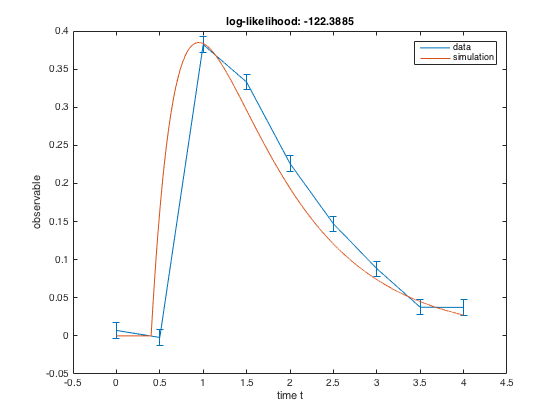
\includegraphics [width=4in]{../../examples/example_5/html/example_model_5_01.png}
\begin{par}
FD
\end{par} \vspace{1em}
\begin{DoxyCode}
eps = 1e-4;
xi = log10(p);
grad_fd_f = NaN(4,1);
grad_fd_b = NaN(4,1);
for ip = 1:4;
    options.sensi = 0;
    xip = xi;
    xip(ip) = xip(ip) + eps;
    solpf = simulate_model_example_5(tout,xip,k,D,options);
    grad_fd_f(ip,1) = (solpf.llh-sol.llh)/eps;
    xip = xi;
    xip(ip) = xip(ip) - eps;
    solpb = simulate_model_example_5(tout,xip,k,D,options);
    grad_fd_b(ip,1) = -(solpb.llh-sol.llh)/eps;
end

figure
plot(abs(grad_fd_f),abs(sol.sllh),'o')
hold on
plot(abs(grad_fd_b),abs(sol.sllh),'o')
set(gca,'XScale','log')
set(gca,'YScale','log')
hold on
axis square
plot([1e2,1e4],[1e2,1e4],'k:')
xlim([1e2,1e4])
ylim([1e2,1e4])
legend('forward FD','backward FD','Location','SouthEast')
xlabel('adjoint sensitivity absolute value of gradient element')
ylabel('computed absolute value of gradient element')
set(gcf,'Position',[100 300 1200 500])
\end{DoxyCode}

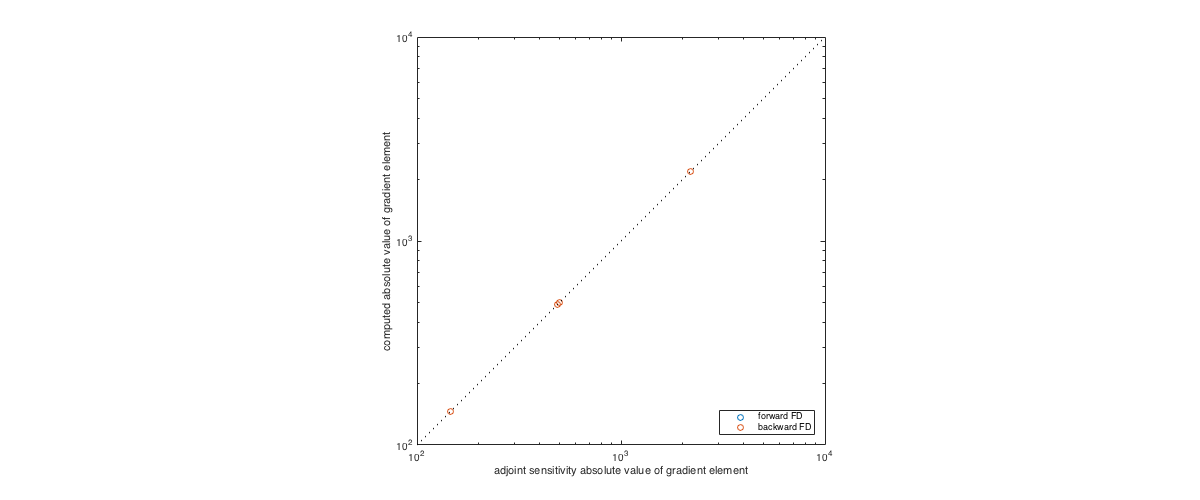
\includegraphics [width=4in]{../../examples/example_5/html/example_model_5_02.png}




     \hypertarget{example6}{}\subsection{Example 6}\label{example6}
\hypertarget{example6_def6}{}\subsubsection{Model Definition}\label{example6_def6}
 
% This LaTeX was auto-generated from MATLAB code.
% To make changes, update the MATLAB code and republish this document.











    
    \begin{DoxyCode}
function [model] = example_model_6_syms()
\end{DoxyCode}
\begin{par}
CVODES OPTIONS
\end{par} \vspace{1em}
\begin{DoxyCode}
% set the default absolute tolerance
model.atol = 1e-8;
% set the default relative tolerance
model.rtol = 1e-8;
% set the default maximum number of integration steps
model.maxsteps = 1e4;
% set the parametrisation of the problem options are 'log', 'log10' and
% 'lin' (default).
model.param = 'log10';
\end{DoxyCode}
\begin{par}
STATES
\end{par} \vspace{1em}
\begin{DoxyCode}
% create state syms
syms x1

% create state vector
x = [ x1];
\end{DoxyCode}
\begin{par}
PARAMETERS ( for these sensitivities will be computed )
\end{par} \vspace{1em}
\begin{DoxyCode}
% create parameter syms
syms p1 p2 p3

% create parameter vector
p = [p1 p2 p3];
\end{DoxyCode}
\begin{par}
SYSTEM EQUATIONS
\end{par} \vspace{1em}
\begin{DoxyCode}
% create symbolic variable for time
syms t

xdot = sym(zeros(size(x)));

% piecewise defined function
xdot(1) = -p1*x1*heaviside(t-2) + p2;
\end{DoxyCode}
\begin{par}
INITIAL CONDITIONS
\end{par} \vspace{1em}
\begin{DoxyCode}
x0 = sym(zeros(size(x)));

x0(1) = p3;
\end{DoxyCode}
\begin{par}
OBSERVALES
\end{par} \vspace{1em}
\begin{DoxyCode}
y = sym(zeros(1,1));

y(1) = x1;
\end{DoxyCode}
\begin{par}
SYSTEM STRUCT
\end{par} \vspace{1em}
\begin{DoxyCode}
model.sym.x = x;
model.sym.xdot = xdot;
model.sym.p = p;
model.sym.x0 = x0;
model.sym.y = y;
\end{DoxyCode}
\begin{DoxyCode}
end
\end{DoxyCode}

         \begin{DoxyCode}ans = 
        atol: 1e-08
        rtol: 1e-08
    maxsteps: 10000
       param: 'log10'
         sym: [1x1 struct]
\end{DoxyCode} 
    



    \hypertarget{example6_simu6}{}\subsubsection{Simulation}\label{example6_simu6}
 
% This LaTeX was auto-generated from MATLAB code.
% To make changes, update the MATLAB code and republish this document.











    
    \begin{DoxyCode}
clear
\end{DoxyCode}
\begin{par}
COMPILATION
\end{par} \vspace{1em}
\begin{DoxyCode}
[exdir,~,~]=fileparts(which('example_model_6.m'));
% compile the model
amiwrap('model_example_6','example_model_6_syms',exdir)
\end{DoxyCode}

         \begin{DoxyCode}Generating model struct ...
Parsing model struct ...
Generating C code ...
headers | wrapfunctions | 
Compiling mex file ...
Building with 'Xcode with Clang'.
MEX completed successfully.
\end{DoxyCode} 
    \begin{par}
SIMULATION
\end{par} \vspace{1em}
\begin{DoxyCode}
% time vector
t = [linspace(0,4,5)];
p = [1.1,0.3,1];
k = [];

% D.Y = [     1.0171
%     1.1761
%     1.1680
%     1.1359
%     1.1778
%     1.3423
%     1.3079
%     1.2784
%     1.4976
%     1.5903
%     1.6585
%     1.4688
%     1.0999
%     1.0128
%     0.7198
%     0.9814
%     0.6755
%     0.5091
%     0.4471
%     0.5249
%     0.3288];


D.Y = [     1.0171
    1.3423
    1.6585
    0.9814
    0.3288];

D.Sigma_Y = 0.1*ones(size(D.Y));


options.sensi = 1;
options.sensi_meth = 'adjoint';
options.cvode_maxsteps = 1e6;
options.cvode_rtol = 1e-12;
options.cvode_atol = 1e-12;
% load mex into memory
[msg] = which('simulate_model_example_6'); % fix for inaccessability problems
sol = simulate_model_example_6(t,log10(p),k,D,options);
\end{DoxyCode}
\begin{par}
Plot
\end{par} \vspace{1em}
\begin{DoxyCode}
figure
subplot(3,1,1)
errorbar(t,D.Y,D.Sigma_Y)
hold on
% plot(t,sol.y)

xlabel('time t')
ylabel('observable')
title(['log-likelihood: ' num2str(sol.llh) ])

y = (p(2)*t + p(3)).*(t<2) + ( (2*p(2)+p(3)-p(2)/p(1))*exp(-p(1)*(t-2))+p(2)/p(1) ).*(t>=2);


tfine = linspace(0,4,100001);
xfine = (p(2)*tfine + 1).*(tfine<2) + ( (2*p(2)+p(3)-p(2)/p(1))*exp(-p(1)*(tfine-2))+p(2)/p(1) ).*(tfine>=2);

mu = zeros(1,length(tfine));
for it = 1:length(t)
if(t(it)<=2)
mu = mu + ((y(it)-D.Y(it))/(D.Sigma_Y(it)^2))*(tfine<=t(it));
else
mu = mu + ((y(it)-D.Y(it))/(D.Sigma_Y(it)^2))*exp(p(1)*(tfine-t(it))).*(tfine<=t(it)).*(tfine>2) + ((y(it)-D.Y(it))/(D.Sigma_Y(it)^2))*exp(p(1)*(2-t(it))).*(tfine<t(it)).*(tfine<=2);
end
end
plot(tfine,xfine)
legend('data','simulation')
xlim([min(t)-0.5,max(t)+0.5])
subplot(3,1,2)
plot(tfine,mu)
ylabel('adjoint')
xlabel('time t')
xlim([min(t)-0.5,max(t)+0.5])

subplot(3,1,3)

plot(fliplr(tfine),-cumsum(fliplr(-mu.*xfine.*(tfine>2)))*p(1)*log(10)*(t(end)/numel(tfine)))
hold on
plot(fliplr(tfine),-cumsum(fliplr(mu))*p(2)*log(10)*(t(end)/numel(tfine)))
plot(tfine,-mu(1)*p(3)*log(10)*(tfine<2))
xlim([min(t)-0.5,max(t)+0.5])
ylabel('integral')
xlabel('time t')

legend('p1','p2','p3')

grad(1,1) = -trapz(tfine,-mu.*xfine.*(tfine>2))*p(1)*log(10);
grad(2,1) = -trapz(tfine,mu)*p(2)*log(10);
grad(3,1) = -mu(1)*p(3)*log(10);

plot(zeros(3,1),grad,'ko')
\end{DoxyCode}

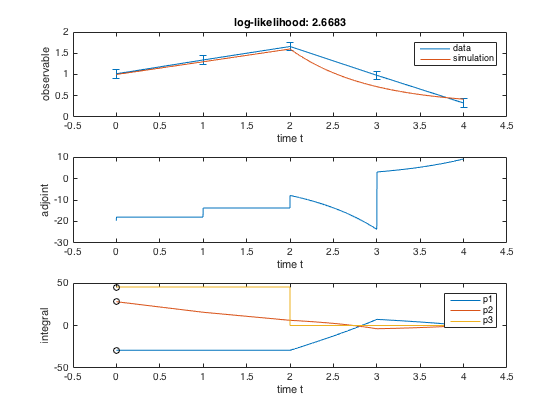
\includegraphics [width=4in]{../../examples/example_6/html/example_model_6_01.png}
\begin{par}
FD
\end{par} \vspace{1em}
\begin{DoxyCode}
eps = 1e-5;
xi = log10(p);
grad_fd_f = NaN(3,1);
grad_fd_b = NaN(3,1);
for ip = 1:3;
    options.sensi = 0;
    xip = xi;
    xip(ip) = xip(ip) + eps;
    solp = simulate_model_example_6(t,xip,k,D,options);
    grad_fd_f(ip,1) = (solp.llh-sol.llh)/eps;
    xip = xi;
    xip(ip) = xip(ip) - eps;
    solp = simulate_model_example_6(t,xip,k,D,options);
    grad_fd_b(ip,1) = -(solp.llh-sol.llh)/eps;
end

figure
plot(abs(grad),abs(grad_fd_f),'o')
hold on
plot(abs(grad),abs(grad_fd_b),'o')
plot(abs(grad),mean([abs(grad_fd_b),abs(grad_fd_f)],2),'o')
plot(abs(grad),abs(sol.sllh),'o')
plot([1e1,1e2],[1e1,1e2],'k:')
set(gca,'XScale','log')
set(gca,'YScale','log')
axis square
legend('forward FD','backward FD','central FD','adjoint sensintivity analysis','Location','SouthEast')
xlabel('analytic absolute value of gradient element')
ylabel('computed absolute value of gradient element')
set(gcf,'Position',[100 300 1200 500])
\end{DoxyCode}

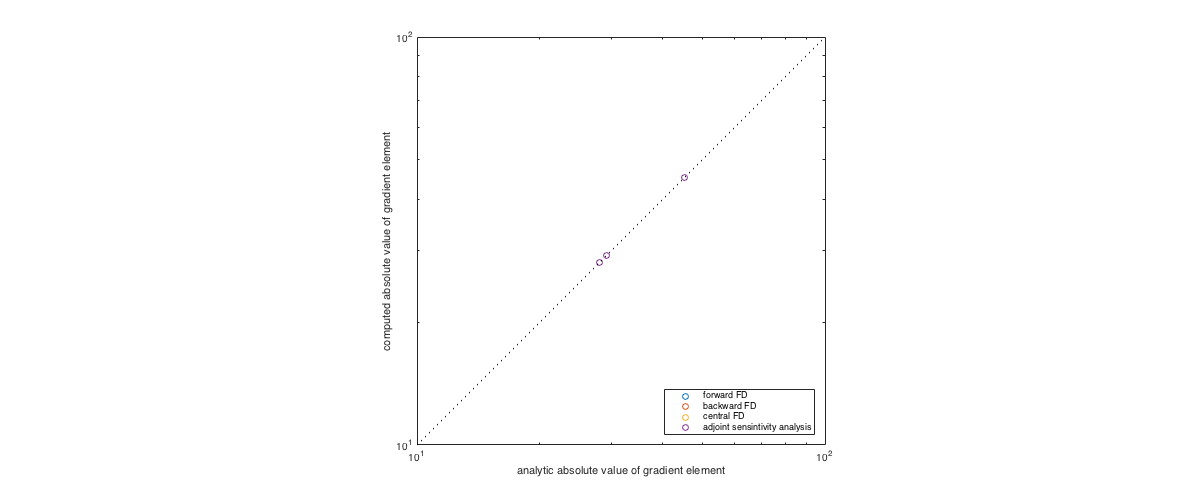
\includegraphics [width=4in]{../../examples/example_6/html/example_model_6_02.png}




     
\section{Code Organization}
\label{code}
\hypertarget{code}{}
In the following we will briefly outline what happens when a model is compiled. For a more detailed description we refer the reader to the documentation of the individual functions.

After specifying a model (see \hyperlink{def_simu_definition}{Model Definition}) the user will typically compile the model by invoking \hyperlink{amiwrap_8m_a183dd11adc4bd525147faa2590ea325b}{amiwrap()}. \hyperlink{amiwrap_8m_a183dd11adc4bd525147faa2590ea325b}{amiwrap()} first instantiates an object of the class \hyperlink{classamimodel}{amimodel}. The properties of this object are initialised based on the user-\/defined model. If the o2flag is active, all subsequent computations will also be carried out on the augmented system, which also includes the equations for forward sensitivities. This allows the computation of second order sensitivities in a forward-\/forward approach. A forward-\/adjoint approach will be implemented in the future.

The sym and fun fields of this object will then be populated by \hyperlink{classamimodel_a68efdc6ed5d618672bea1556209e5568}{amimodel\+::parse\+Model()}. The \hyperlink{classamimodel_a3c48fff3d28406486a4f1b5e18da7ca6}{amimodel\+::sym} field contains all necessary symbolic expression while the \hyperlink{classamimodel_a743fa290dbc0a67a3843d5ab0426e9b4}{amimodel\+::fun} field will contain flags for all functions whether the C code for a certain function needs to be regenerated or not. The set of functions to be considered will depend on the user specification of the model fields \hyperlink{classamimodel_ab6d500b41cf50693452415caca31d32e}{amimodel\+::adjoint} and \hyperlink{classamimodel_a81e42e48c9c72814166c8f7cd414ce24}{amimodel\+::forward} (see \hyperlink{def_simu_options}{Options}) as well as the employed solver (C\+V\+O\+D\+E\+S or I\+D\+A\+S, see \hyperlink{def_simu_rhs}{Differential Equation}). For all considered functions \hyperlink{classamimodel_a68efdc6ed5d618672bea1556209e5568}{amimodel\+::parse\+Model()} will check their dependencies via \hyperlink{classamimodel_aa04dcfc1d2188cae948a75ebd46a6e03}{amimodel\+::check\+Deps()}. These dependencies are a subset of the user-\/specified fields of \hyperlink{classamimodel_a3c48fff3d28406486a4f1b5e18da7ca6}{amimodel\+::sym} (see \hyperlink{def_simu_attach}{Attach to Model Struct}). \hyperlink{classamimodel_a68efdc6ed5d618672bea1556209e5568}{amimodel\+::parse\+Model()} compares the hashes of all dependencies against the \hyperlink{classamimodel_aafe6335df413dd688a2f44efba012cf1}{amimodel\+::\+H\+Table} of possible previous compilations and will only compute necessary symbolic expressions if changes in these fields occured. If changes in the dependencies occured, also the respective subfield in \hyperlink{classamimodel_a743fa290dbc0a67a3843d5ab0426e9b4}{amimodel\+::fun} be set to 1, indicating the necessity of regeneration of respective C code.

For all functions for which \hyperlink{classamimodel_a743fa290dbc0a67a3843d5ab0426e9b4}{amimodel\+::fun} is set to 1, \hyperlink{classamimodel_af2ce5001c2320c95471ecb8c3d73bdbb}{amimodel\+::generate\+C()} will generate C files. These files together with their respective header files will be placed in \$\+A\+M\+I\+C\+I\+D\+I\+R/models/{\itshape modelname}. \hyperlink{classamimodel_af2ce5001c2320c95471ecb8c3d73bdbb}{amimodel\+::generate\+C()} will also generate wrapfunctions.\+h and wrapfunctions.\+c. These files define and declare model unspecific wrapper functions around model specific functions. This construction allows us to use to build multiple different models against the same simulation routines by linking different realisations of these wrapper functions.

All the generated C functions are subsequently compiled by \hyperlink{classamimodel_ad1339463ebc3a2e6c6aeda6f63f1b4ed}{amimodel\+::compile\+C()}. For all functions individual object files are created to reduce the computation cost of code optimization. Moreover necessary code from sundials and Suite\+Sparse is compiled as object files and placed in /models/{\itshape mexext}, where mexext stands for the string returned by matlab to the command mexext. The mex simulation file is compiled from \hyperlink{amiwrap_8c}{amiwrap.\+c}, linked against all object necessary of sundials, Suite\+Sparse and model specific functions. Depending on the required solver, the compilation will either include \hyperlink{cvodewrap_8h_source}{cvodewrap.\+h} or \hyperlink{idawrap_8h_source}{idawrap.\+h}. These files implement solver specific realisations of the A\+M\+I... functions used in \hyperlink{amiwrap_8c}{amiwrap.\+c} and \hyperlink{amici_8c}{amici.\+c}. This allows the use of the same simulation routines for both C\+V\+O\+D\+E\+S and I\+D\+A\+S. 
\section{Hierarchical Index}
\subsection{Class Hierarchy}
This inheritance list is sorted roughly, but not completely, alphabetically\+:\begin{DoxyCompactList}
\item \contentsline{section}{amievent}{\pageref{classamievent}}{}
\item \contentsline{section}{amifun}{\pageref{classamifun}}{}
\item \contentsline{section}{Exp\+Data}{\pageref{struct_exp_data}}{}
\item \contentsline{section}{fun\+Test}{\pageref{classfun_test}}{}
\item handle\begin{DoxyCompactList}
\item \contentsline{section}{amidata}{\pageref{classamidata}}{}
\item \contentsline{section}{amimodel}{\pageref{classamimodel}}{}
\item \contentsline{section}{S\+B\+M\+Lode}{\pageref{class_s_b_m_lode}}{}
\end{DoxyCompactList}
\item Set\+Get\begin{DoxyCompactList}
\item \contentsline{section}{amioption}{\pageref{classamioption}}{}
\end{DoxyCompactList}
\item \contentsline{section}{model\+Test}{\pageref{classmodel_test}}{}
\item \contentsline{section}{Return\+Data}{\pageref{struct_return_data}}{}
\item sym\begin{DoxyCompactList}
\item \contentsline{section}{optsym}{\pageref{classoptsym}}{}
\end{DoxyCompactList}
\item \contentsline{section}{Temp\+Data}{\pageref{struct_temp_data}}{}
\item \contentsline{section}{User\+Data}{\pageref{struct_user_data}}{}
\end{DoxyCompactList}

\section{Class Index}
\subsection{Class List}
Here are the classes, structs, unions and interfaces with brief descriptions\+:\begin{DoxyCompactList}
\item\contentsline{section}{\hyperlink{classamievent}{amievent} \\*Amievent class defines the prototype for all events which later on will be transformed into C code }{\pageref{classamievent}}{}
\item\contentsline{section}{\hyperlink{classamifun}{amifun} \\*Amifun class defines the prototype for all functions which later on will be transformed into C code }{\pageref{classamifun}}{}
\item\contentsline{section}{\hyperlink{classamimodel}{amimodel} \\*Amimodel is the object in which all model definitions are stored }{\pageref{classamimodel}}{}
\item\contentsline{section}{\hyperlink{struct_exp_data}{Exp\+Data} \\*Struct that carries all information about experimental data }{\pageref{struct_exp_data}}{}
\item\contentsline{section}{\hyperlink{struct_return_data}{Return\+Data} \\*Struct that stores all data which is later returned by the mex function }{\pageref{struct_return_data}}{}
\item\contentsline{section}{\hyperlink{struct_temp_data}{Temp\+Data} \\*Struct that provides temporary storage for different variables }{\pageref{struct_temp_data}}{}
\item\contentsline{section}{\hyperlink{struct_user_data}{User\+Data} \\*Struct that stores all user provided data }{\pageref{struct_user_data}}{}
\end{DoxyCompactList}

\section{Class Documentation}
\hypertarget{classamidata}{}\doxysubsection{amidata Class Reference}
\label{classamidata}\index{amidata@{amidata}}


AMIDATA provides a data container to pass experimental data to the simulation routine for likelihood computation. when any of the properties are updated, the class automatically checks consistency of dimension and updates related properties and initialises them with Na\+Ns.  




Inheritance diagram for amidata\+:
\nopagebreak
\begin{figure}[H]
\begin{center}
\leavevmode
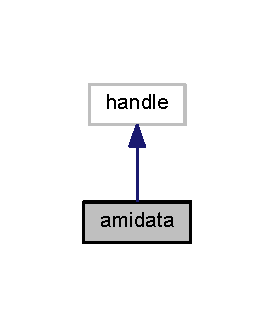
\includegraphics[width=131pt]{classamidata__inherit__graph}
\end{center}
\end{figure}
\doxysubsubsection*{Public Member Functions}
\begin{DoxyCompactItemize}
\item 
\mbox{\hyperlink{classamidata_a28c05d6ebaf7baa45ff8b2465ce07b3f}{amidata}} (matlabtypesubstitute varargin)
\begin{DoxyCompactList}\small\item\em amidata creates an amidata container for experimental data with specified dimensions amidata. \end{DoxyCompactList}\end{DoxyCompactItemize}
\doxysubsubsection*{Public Attributes}
\begin{DoxyCompactItemize}
\item 
matlabtypesubstitute \mbox{\hyperlink{classamidata_a03cfcdd983bff4aef77268b785b28345}{nt}} = 0
\begin{DoxyCompactList}\small\item\em number of timepoints \end{DoxyCompactList}\item 
matlabtypesubstitute \mbox{\hyperlink{classamidata_a289ca425eb368f1d582b6be2be0d3dfc}{ny}} = 0
\begin{DoxyCompactList}\small\item\em number of observables \end{DoxyCompactList}\item 
matlabtypesubstitute \mbox{\hyperlink{classamidata_a79f11413e5bfe18a0e71e17574399ad5}{nz}} = 0
\begin{DoxyCompactList}\small\item\em number of event observables \end{DoxyCompactList}\item 
matlabtypesubstitute \mbox{\hyperlink{classamidata_aaca25d624cf863f786f67137c62aa11d}{ne}} = 0
\begin{DoxyCompactList}\small\item\em number of events \end{DoxyCompactList}\item 
matlabtypesubstitute \mbox{\hyperlink{classamidata_afd6bea572754e0c3c320664bdccf0200}{nk}} = 0
\begin{DoxyCompactList}\small\item\em number of conditions/constants \end{DoxyCompactList}\item 
matlabtypesubstitute \mbox{\hyperlink{classamidata_aaccc9105df5383111407fd5b41255e23}{t}} = double.\+empty(\char`\"{}\char`\"{})
\begin{DoxyCompactList}\small\item\em timepoints of observations \end{DoxyCompactList}\item 
matlabtypesubstitute \mbox{\hyperlink{classamidata_a0867f43e27585e019c13f7f4b7c4ab6b}{Y}} = double.\+empty(\char`\"{}\char`\"{})
\begin{DoxyCompactList}\small\item\em observations \end{DoxyCompactList}\item 
matlabtypesubstitute \mbox{\hyperlink{classamidata_a4bd82fb17b03a0039c2f0347ec8dc393}{Sigma\+\_\+Y}} = double.\+empty(\char`\"{}\char`\"{})
\begin{DoxyCompactList}\small\item\em standard deviation of observations \end{DoxyCompactList}\item 
matlabtypesubstitute \mbox{\hyperlink{classamidata_adc18d83abfd9f87d396e8fd6b6ac0fe1}{Z}} = double.\+empty(\char`\"{}\char`\"{})
\begin{DoxyCompactList}\small\item\em event observations \end{DoxyCompactList}\item 
matlabtypesubstitute \mbox{\hyperlink{classamidata_a77b1f0ddcfbfb895b17d62a414d35673}{Sigma\+\_\+Z}} = double.\+empty(\char`\"{}\char`\"{})
\begin{DoxyCompactList}\small\item\em standard deviation of event observations \end{DoxyCompactList}\item 
matlabtypesubstitute \mbox{\hyperlink{classamidata_a4824b91cc0e6b5f112bdd8049af4d7d6}{condition}} = double.\+empty(\char`\"{}\char`\"{})
\begin{DoxyCompactList}\small\item\em experimental condition \end{DoxyCompactList}\item 
matlabtypesubstitute \mbox{\hyperlink{classamidata_af7a0dbd9e6e3f3cb15ae008beeaf841a}{condition\+Preequilibration}} = double.\+empty(\char`\"{}\char`\"{})
\begin{DoxyCompactList}\small\item\em experimental condition for preequilibration \end{DoxyCompactList}\item 
matlabtypesubstitute \mbox{\hyperlink{classamidata_ac06982c517a66355434a7461d51b0994}{reinitialize\+States}} = false
\begin{DoxyCompactList}\small\item\em reinitialize states based on fixed parameters after preeq.? \end{DoxyCompactList}\end{DoxyCompactItemize}


\doxysubsubsection{Detailed Description}


Definition at line 17 of file amidata.\+m.



\doxysubsubsection{Constructor \& Destructor Documentation}
\mbox{\Hypertarget{classamidata_a28c05d6ebaf7baa45ff8b2465ce07b3f}\label{classamidata_a28c05d6ebaf7baa45ff8b2465ce07b3f}} 
\index{amidata@{amidata}!amidata@{amidata}}
\index{amidata@{amidata}!amidata@{amidata}}
\doxyparagraph{\texorpdfstring{amidata()}{amidata()}}
{\footnotesize\ttfamily \mbox{\hyperlink{classamidata}{amidata}} (\begin{DoxyParamCaption}\item[{matlabtypesubstitute}]{varargin }\end{DoxyParamCaption})}

AMIDATA(amidata) creates a copy of the input container

AMIDATA(struct) tries to creates an amidata container from the input struct. the struct should have the following \begin{DoxyParagraph}{fields}
t \mbox{[}nt,1\mbox{]} Y \mbox{[}nt,ny\mbox{]} Sigma\+\_\+Y \mbox{[}nt,ny\mbox{]} Z \mbox{[}ne,nz\mbox{]} Sigma\+\_\+Z \mbox{[}ne,nz\mbox{]} condition \mbox{[}nk,1\mbox{]} condition\+Preequilibration \mbox{[}nk,1\mbox{]} if some fields are missing the function will try to initialise them with Na\+Ns with consistent dimensions
\end{DoxyParagraph}
AMIDATA(nt,ny,nz,ne,nk) constructs an empty data container with in the provided dimensions intialised with Na\+Ns


\begin{DoxyParams}{Parameters}
{\em varargin} & ~\newline
 \\
\hline
\end{DoxyParams}


Definition at line 138 of file amidata.\+m.



\doxysubsubsection{Member Data Documentation}
\mbox{\Hypertarget{classamidata_a03cfcdd983bff4aef77268b785b28345}\label{classamidata_a03cfcdd983bff4aef77268b785b28345}} 
\index{amidata@{amidata}!nt@{nt}}
\index{nt@{nt}!amidata@{amidata}}
\doxyparagraph{\texorpdfstring{nt}{nt}}
{\footnotesize\ttfamily nt = 0}

~\newline
{\bfseries{Default\+:}} 0

\begin{DoxyNote}{Note}
This property has custom functionality when its value is changed. 
\end{DoxyNote}


Definition at line 31 of file amidata.\+m.

\mbox{\Hypertarget{classamidata_a289ca425eb368f1d582b6be2be0d3dfc}\label{classamidata_a289ca425eb368f1d582b6be2be0d3dfc}} 
\index{amidata@{amidata}!ny@{ny}}
\index{ny@{ny}!amidata@{amidata}}
\doxyparagraph{\texorpdfstring{ny}{ny}}
{\footnotesize\ttfamily ny = 0}

~\newline
{\bfseries{Default\+:}} 0

\begin{DoxyNote}{Note}
This property has custom functionality when its value is changed. 
\end{DoxyNote}


Definition at line 39 of file amidata.\+m.

\mbox{\Hypertarget{classamidata_a79f11413e5bfe18a0e71e17574399ad5}\label{classamidata_a79f11413e5bfe18a0e71e17574399ad5}} 
\index{amidata@{amidata}!nz@{nz}}
\index{nz@{nz}!amidata@{amidata}}
\doxyparagraph{\texorpdfstring{nz}{nz}}
{\footnotesize\ttfamily nz = 0}

~\newline
{\bfseries{Default\+:}} 0

\begin{DoxyNote}{Note}
This property has custom functionality when its value is changed. 
\end{DoxyNote}


Definition at line 47 of file amidata.\+m.

\mbox{\Hypertarget{classamidata_aaca25d624cf863f786f67137c62aa11d}\label{classamidata_aaca25d624cf863f786f67137c62aa11d}} 
\index{amidata@{amidata}!ne@{ne}}
\index{ne@{ne}!amidata@{amidata}}
\doxyparagraph{\texorpdfstring{ne}{ne}}
{\footnotesize\ttfamily ne = 0}

~\newline
{\bfseries{Default\+:}} 0

\begin{DoxyNote}{Note}
This property has custom functionality when its value is changed. 
\end{DoxyNote}


Definition at line 55 of file amidata.\+m.

\mbox{\Hypertarget{classamidata_afd6bea572754e0c3c320664bdccf0200}\label{classamidata_afd6bea572754e0c3c320664bdccf0200}} 
\index{amidata@{amidata}!nk@{nk}}
\index{nk@{nk}!amidata@{amidata}}
\doxyparagraph{\texorpdfstring{nk}{nk}}
{\footnotesize\ttfamily nk = 0}

~\newline
{\bfseries{Default\+:}} 0

\begin{DoxyNote}{Note}
This property has custom functionality when its value is changed. 
\end{DoxyNote}


Definition at line 63 of file amidata.\+m.

\mbox{\Hypertarget{classamidata_aaccc9105df5383111407fd5b41255e23}\label{classamidata_aaccc9105df5383111407fd5b41255e23}} 
\index{amidata@{amidata}!t@{t}}
\index{t@{t}!amidata@{amidata}}
\doxyparagraph{\texorpdfstring{t}{t}}
{\footnotesize\ttfamily t = double.\+empty(\char`\"{}\char`\"{})}

~\newline
{\bfseries{Default\+:}} double.\+empty(\char`\"{}\char`\"{})

\begin{DoxyNote}{Note}
This property has custom functionality when its value is changed. 
\end{DoxyNote}


Definition at line 71 of file amidata.\+m.

\mbox{\Hypertarget{classamidata_a0867f43e27585e019c13f7f4b7c4ab6b}\label{classamidata_a0867f43e27585e019c13f7f4b7c4ab6b}} 
\index{amidata@{amidata}!Y@{Y}}
\index{Y@{Y}!amidata@{amidata}}
\doxyparagraph{\texorpdfstring{Y}{Y}}
{\footnotesize\ttfamily Y = double.\+empty(\char`\"{}\char`\"{})}

~\newline
{\bfseries{Default\+:}} double.\+empty(\char`\"{}\char`\"{})

\begin{DoxyNote}{Note}
This property has custom functionality when its value is changed. 
\end{DoxyNote}


Definition at line 79 of file amidata.\+m.

\mbox{\Hypertarget{classamidata_a4bd82fb17b03a0039c2f0347ec8dc393}\label{classamidata_a4bd82fb17b03a0039c2f0347ec8dc393}} 
\index{amidata@{amidata}!Sigma\_Y@{Sigma\_Y}}
\index{Sigma\_Y@{Sigma\_Y}!amidata@{amidata}}
\doxyparagraph{\texorpdfstring{Sigma\_Y}{Sigma\_Y}}
{\footnotesize\ttfamily Sigma\+\_\+Y = double.\+empty(\char`\"{}\char`\"{})}

~\newline
{\bfseries{Default\+:}} double.\+empty(\char`\"{}\char`\"{})

\begin{DoxyNote}{Note}
This property has custom functionality when its value is changed. 
\end{DoxyNote}


Definition at line 87 of file amidata.\+m.

\mbox{\Hypertarget{classamidata_adc18d83abfd9f87d396e8fd6b6ac0fe1}\label{classamidata_adc18d83abfd9f87d396e8fd6b6ac0fe1}} 
\index{amidata@{amidata}!Z@{Z}}
\index{Z@{Z}!amidata@{amidata}}
\doxyparagraph{\texorpdfstring{Z}{Z}}
{\footnotesize\ttfamily Z = double.\+empty(\char`\"{}\char`\"{})}

~\newline
{\bfseries{Default\+:}} double.\+empty(\char`\"{}\char`\"{})

\begin{DoxyNote}{Note}
This property has custom functionality when its value is changed. 
\end{DoxyNote}


Definition at line 95 of file amidata.\+m.

\mbox{\Hypertarget{classamidata_a77b1f0ddcfbfb895b17d62a414d35673}\label{classamidata_a77b1f0ddcfbfb895b17d62a414d35673}} 
\index{amidata@{amidata}!Sigma\_Z@{Sigma\_Z}}
\index{Sigma\_Z@{Sigma\_Z}!amidata@{amidata}}
\doxyparagraph{\texorpdfstring{Sigma\_Z}{Sigma\_Z}}
{\footnotesize\ttfamily Sigma\+\_\+Z = double.\+empty(\char`\"{}\char`\"{})}

~\newline
{\bfseries{Default\+:}} double.\+empty(\char`\"{}\char`\"{})

\begin{DoxyNote}{Note}
This property has custom functionality when its value is changed. 
\end{DoxyNote}


Definition at line 103 of file amidata.\+m.

\mbox{\Hypertarget{classamidata_a4824b91cc0e6b5f112bdd8049af4d7d6}\label{classamidata_a4824b91cc0e6b5f112bdd8049af4d7d6}} 
\index{amidata@{amidata}!condition@{condition}}
\index{condition@{condition}!amidata@{amidata}}
\doxyparagraph{\texorpdfstring{condition}{condition}}
{\footnotesize\ttfamily condition = double.\+empty(\char`\"{}\char`\"{})}

~\newline
{\bfseries{Default\+:}} double.\+empty(\char`\"{}\char`\"{})

\begin{DoxyNote}{Note}
This property has custom functionality when its value is changed. 
\end{DoxyNote}


Definition at line 111 of file amidata.\+m.

\mbox{\Hypertarget{classamidata_af7a0dbd9e6e3f3cb15ae008beeaf841a}\label{classamidata_af7a0dbd9e6e3f3cb15ae008beeaf841a}} 
\index{amidata@{amidata}!conditionPreequilibration@{conditionPreequilibration}}
\index{conditionPreequilibration@{conditionPreequilibration}!amidata@{amidata}}
\doxyparagraph{\texorpdfstring{conditionPreequilibration}{conditionPreequilibration}}
{\footnotesize\ttfamily condition\+Preequilibration = double.\+empty(\char`\"{}\char`\"{})}

~\newline
{\bfseries{Default\+:}} double.\+empty(\char`\"{}\char`\"{})

\begin{DoxyNote}{Note}
This property has custom functionality when its value is changed. 
\end{DoxyNote}


Definition at line 119 of file amidata.\+m.

\mbox{\Hypertarget{classamidata_ac06982c517a66355434a7461d51b0994}\label{classamidata_ac06982c517a66355434a7461d51b0994}} 
\index{amidata@{amidata}!reinitializeStates@{reinitializeStates}}
\index{reinitializeStates@{reinitializeStates}!amidata@{amidata}}
\doxyparagraph{\texorpdfstring{reinitializeStates}{reinitializeStates}}
{\footnotesize\ttfamily reinitialize\+States = false}

~\newline
{\bfseries{Default\+:}} false 

Definition at line 127 of file amidata.\+m.


\hypertarget{classamievent}{}\subsection{amievent Class Reference}
\label{classamievent}\index{amievent@{amievent}}


A\+M\+I\+E\+V\+E\+N\+T defines events which later on will be transformed into appropriate C code.  


\subsubsection*{Public Member Functions}
\begin{DoxyCompactItemize}
\item 
\hyperlink{classamievent_a64b7d5a2d9dc65a982f1f9812949b865}{amievent} (matlabtypesubstitute \hyperlink{classamievent_ae194cb817eae4085f8023885100c68dd}{trigger}, matlabtypesubstitute \hyperlink{classamievent_ab9227561ac246ee4b70f9e65c25ffda7}{bolus}, matlabtypesubstitute \hyperlink{classamievent_a25ed1bcb423b0b7200f485fc5ff71c8e}{z})
\begin{DoxyCompactList}\small\item\em amievent constructs an amievent object from the provided input. \end{DoxyCompactList}\item 
mlhs\+Inner\+Subst$<$ matlabtypesubstitute $>$ \hyperlink{classamievent_aef1933f186f69e58e2aa1b00d01f75e7}{set\+Hflag} (\+::double \hyperlink{classamievent_ab98347b5ce6fbe7bd007030346b88575}{hflag})
\begin{DoxyCompactList}\small\item\em gethflag sets the hflag property. \end{DoxyCompactList}\end{DoxyCompactItemize}
\subsubsection*{Public Attributes}
\begin{DoxyCompactItemize}
\item 
\+::symbolic \hyperlink{classamievent_ae194cb817eae4085f8023885100c68dd}{trigger} = sym.\+empty(\char`\"{}\char`\"{})
\begin{DoxyCompactList}\small\item\em the trigger function activates the event on every zero crossing \end{DoxyCompactList}\item 
\+::symbolic \hyperlink{classamievent_ab9227561ac246ee4b70f9e65c25ffda7}{bolus} = sym.\+empty(\char`\"{}\char`\"{})
\begin{DoxyCompactList}\small\item\em the bolus function defines the change in states that is applied on every event occurence \end{DoxyCompactList}\item 
\+::symbolic \hyperlink{classamievent_a25ed1bcb423b0b7200f485fc5ff71c8e}{z} = sym.\+empty(\char`\"{}\char`\"{})
\begin{DoxyCompactList}\small\item\em output function for the event \end{DoxyCompactList}\item 
matlabtypesubstitute \hyperlink{classamievent_ab98347b5ce6fbe7bd007030346b88575}{hflag} = logical.\+empty(\char`\"{}\char`\"{})
\begin{DoxyCompactList}\small\item\em flag indicating that a heaviside function is present, this helps to speed up symbolic computations \end{DoxyCompactList}\end{DoxyCompactItemize}


\subsubsection{Detailed Description}


Definition at line 17 of file amievent.\+m.



\subsubsection{Constructor \& Destructor Documentation}
\hypertarget{classamievent_a64b7d5a2d9dc65a982f1f9812949b865}{}\index{amievent@{amievent}!amievent@{amievent}}
\index{amievent@{amievent}!amievent@{amievent}}
\paragraph[{amievent(matlabtypesubstitute trigger, matlabtypesubstitute bolus, matlabtypesubstitute z)}]{\setlength{\rightskip}{0pt plus 5cm}{\bf amievent} (
\begin{DoxyParamCaption}
\item[{matlabtypesubstitute}]{trigger, }
\item[{matlabtypesubstitute}]{bolus, }
\item[{matlabtypesubstitute}]{z}
\end{DoxyParamCaption}
)}\label{classamievent_a64b7d5a2d9dc65a982f1f9812949b865}

\begin{DoxyParams}{Parameters}
{\em trigger} & trigger function, the event will be triggered on at all roots of this function \\
\hline
{\em bolus} & the bolus that will be added to all states on every occurence of the event \\
\hline
{\em z} & the event output that will be reported on every occurence of the event \\
\hline
\end{DoxyParams}


Definition at line 75 of file amievent.\+m.



\subsubsection{Member Function Documentation}
\hypertarget{classamievent_aef1933f186f69e58e2aa1b00d01f75e7}{}\index{amievent@{amievent}!set\+Hflag@{set\+Hflag}}
\index{set\+Hflag@{set\+Hflag}!amievent@{amievent}}
\paragraph[{set\+Hflag(\+::double hflag)}]{\setlength{\rightskip}{0pt plus 5cm}mlhs\+Inner\+Subst$<$\+::{\bf amievent} $>$ set\+Hflag (
\begin{DoxyParamCaption}
\item[{\+::double}]{hflag}
\end{DoxyParamCaption}
)}\label{classamievent_aef1933f186f69e58e2aa1b00d01f75e7}

\begin{DoxyParams}{Parameters}
{\em hflag} & value for the hflag property\\
\hline
\end{DoxyParams}

\begin{DoxyRetVals}{Return values}
{\em this} & updated event definition object \\
\hline
\end{DoxyRetVals}


Definition at line 18 of file set\+Hflag.\+m.



Here is the caller graph for this function\+:\nopagebreak
\begin{figure}[H]
\begin{center}
\leavevmode
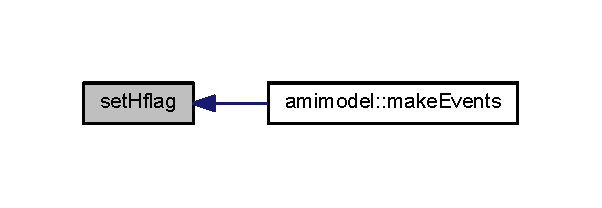
\includegraphics[width=289pt]{classamievent_aef1933f186f69e58e2aa1b00d01f75e7_icgraph}
\end{center}
\end{figure}




\subsubsection{Member Data Documentation}
\hypertarget{classamievent_ae194cb817eae4085f8023885100c68dd}{}\index{amievent@{amievent}!trigger@{trigger}}
\index{trigger@{trigger}!amievent@{amievent}}
\paragraph[{trigger}]{\setlength{\rightskip}{0pt plus 5cm}trigger = sym.\+empty(\char`\"{}\char`\"{})}\label{classamievent_ae194cb817eae4085f8023885100c68dd}
\begin{DoxyNote}{Note}
This property has non-\/standard access specifiers\+: {\ttfamily Set\+Access = Private, Get\+Access = Public} 

\href{http://www.mathworks.com/help/matlab/matlab_oop/property-attributes.html}{\tt Matlab documentation of property attributes.} ~\newline
{\bfseries Default\+:} sym.\+empty(\char`\"{}\char`\"{}) 
\end{DoxyNote}


Definition at line 27 of file amievent.\+m.

\hypertarget{classamievent_ab9227561ac246ee4b70f9e65c25ffda7}{}\index{amievent@{amievent}!bolus@{bolus}}
\index{bolus@{bolus}!amievent@{amievent}}
\paragraph[{bolus}]{\setlength{\rightskip}{0pt plus 5cm}bolus = sym.\+empty(\char`\"{}\char`\"{})}\label{classamievent_ab9227561ac246ee4b70f9e65c25ffda7}
\begin{DoxyNote}{Note}
This property has non-\/standard access specifiers\+: {\ttfamily Set\+Access = Private, Get\+Access = Public} 

\href{http://www.mathworks.com/help/matlab/matlab_oop/property-attributes.html}{\tt Matlab documentation of property attributes.} ~\newline
{\bfseries Default\+:} sym.\+empty(\char`\"{}\char`\"{}) 
\end{DoxyNote}


Definition at line 38 of file amievent.\+m.

\hypertarget{classamievent_a25ed1bcb423b0b7200f485fc5ff71c8e}{}\index{amievent@{amievent}!z@{z}}
\index{z@{z}!amievent@{amievent}}
\paragraph[{z}]{\setlength{\rightskip}{0pt plus 5cm}z = sym.\+empty(\char`\"{}\char`\"{})}\label{classamievent_a25ed1bcb423b0b7200f485fc5ff71c8e}
\begin{DoxyNote}{Note}
This property has non-\/standard access specifiers\+: {\ttfamily Set\+Access = Private, Get\+Access = Public} 

\href{http://www.mathworks.com/help/matlab/matlab_oop/property-attributes.html}{\tt Matlab documentation of property attributes.} ~\newline
{\bfseries Default\+:} sym.\+empty(\char`\"{}\char`\"{}) 
\end{DoxyNote}


Definition at line 49 of file amievent.\+m.

\hypertarget{classamievent_ab98347b5ce6fbe7bd007030346b88575}{}\index{amievent@{amievent}!hflag@{hflag}}
\index{hflag@{hflag}!amievent@{amievent}}
\paragraph[{hflag}]{\setlength{\rightskip}{0pt plus 5cm}hflag = logical.\+empty(\char`\"{}\char`\"{})}\label{classamievent_ab98347b5ce6fbe7bd007030346b88575}
\begin{DoxyNote}{Note}
This property has non-\/standard access specifiers\+: {\ttfamily Set\+Access = Private, Get\+Access = Public} 

\href{http://www.mathworks.com/help/matlab/matlab_oop/property-attributes.html}{\tt Matlab documentation of property attributes.} ~\newline
{\bfseries Default\+:} logical.\+empty(\char`\"{}\char`\"{}) 
\end{DoxyNote}


Definition at line 60 of file amievent.\+m.


\hypertarget{classamifun}{}\doxysubsection{amifun Class Reference}
\label{classamifun}\index{amifun@{amifun}}


A\+M\+I\+F\+UN defines functions which later on will be transformed into appropriate C code.  


\doxysubsubsection*{Public Member Functions}
\begin{DoxyCompactItemize}
\item 
\mbox{\hyperlink{classamifun_a609e744c18813bc24f360b8cc5150344}{amifun}} (matlabtypesubstitute \mbox{\hyperlink{classamifun_a484b54379bc8b29b6ce65d84966ea4c4}{funstr}}, matlabtypesubstitute model)
\begin{DoxyCompactList}\small\item\em amievent constructs an amifun object from the provided input. \end{DoxyCompactList}\item 
noret\+::substitute \mbox{\hyperlink{classamifun_a7845c1193d9a963f7bb9802f1eeefac7}{write\+Ccode\+\_\+sensi}} (\+::\mbox{\hyperlink{classamimodel}{amimodel}} model,\+::fileid fid)
\begin{DoxyCompactList}\small\item\em write\+Ccode\+\_\+sensi is a wrapper for write\+Ccode which loops over parameters and reduces overhead by check nonzero values \end{DoxyCompactList}\item 
noret\+::substitute \mbox{\hyperlink{classamifun_a8e48f2842268ff64ca32db8eb4b69377}{write\+Ccode}} (\+::\mbox{\hyperlink{classamimodel}{amimodel}} model,\+::fileid fid)
\begin{DoxyCompactList}\small\item\em write\+Ccode is a wrapper for gccode which initialises data and reduces overhead by check nonzero values \end{DoxyCompactList}\item 
noret\+::substitute \mbox{\hyperlink{classamifun_a9b041ce0ffcfab125b5db3ed5ca847a2}{write\+Mcode}} (\+::\mbox{\hyperlink{classamimodel}{amimodel}} model)
\begin{DoxyCompactList}\small\item\em write\+Mcode generates matlab evaluable code for specific model functions \end{DoxyCompactList}\item 
noret\+::substitute \mbox{\hyperlink{classamifun_a05444f498e657a0010f6b539bc9c6596}{gccode}} (\+::\mbox{\hyperlink{classamimodel}{amimodel}} model,\+::fileid fid)
\begin{DoxyCompactList}\small\item\em gccode transforms symbolic expressions into c code and writes the respective expression into a specified file \end{DoxyCompactList}\item 
mlhs\+Inner\+Subst$<$ matlabtypesubstitute $>$ \mbox{\hyperlink{classamifun_a1cb97b695ab609e1655ec1067b140b70}{get\+Deps}} (\+::\mbox{\hyperlink{classamimodel}{amimodel}} model)
\begin{DoxyCompactList}\small\item\em get\+Deps populates the sensiflag for the requested function \end{DoxyCompactList}\item 
mlhs\+Inner\+Subst$<$ matlabtypesubstitute $>$ \mbox{\hyperlink{classamifun_a4b16e7670c0d60e530545e58628bde3f}{get\+Args}} (\+::\mbox{\hyperlink{classamimodel}{amimodel}} model)
\begin{DoxyCompactList}\small\item\em get\+F\+Args populates the fargstr property with the argument string of the respective model function (if applicable). model functions are not wrapped versions of functions which have a model specific name and for which the call is solver specific. \end{DoxyCompactList}\item 
mlhs\+Inner\+Subst$<$ matlabtypesubstitute $>$ \mbox{\hyperlink{classamifun_a3ae210044df5eb51e2f9280d03b86c3c}{get\+N\+Vecs}} ()
\begin{DoxyCompactList}\small\item\em getfunargs populates the nvecs property with the names of the N\+\_\+\+Vector elements which are required in the execution of the function (if applicable). the information is directly extracted from the argument string \end{DoxyCompactList}\item 
mlhs\+Inner\+Subst$<$ matlabtypesubstitute $>$ \mbox{\hyperlink{classamifun_a969775839d9d32ff4a0ba70395117ca7}{get\+C\+Var}} ()
\begin{DoxyCompactList}\small\item\em get\+C\+Var populates the cvar property \end{DoxyCompactList}\item 
mlhs\+Inner\+Subst$<$ matlabtypesubstitute $>$ \mbox{\hyperlink{classamifun_ac60147b051aa541057d0da18a78582a8}{get\+Sensi\+Flag}} ()
\begin{DoxyCompactList}\small\item\em get\+Sensi\+Flag populates the sensiflag property \end{DoxyCompactList}\item 
mlhs\+Subst$<$ mlhs\+Inner\+Subst$<$ matlabtypesubstitute $>$,mlhs\+Inner\+Subst$<$\+::\mbox{\hyperlink{classamimodel}{amimodel}} $>$ $>$ \mbox{\hyperlink{classamifun_a44e49602645d85f94841f38e4673fa1a}{get\+Syms}} (\+::\mbox{\hyperlink{classamimodel}{amimodel}} model)
\begin{DoxyCompactList}\small\item\em get\+Syms computes the symbolic expression for the requested function \end{DoxyCompactList}\end{DoxyCompactItemize}
\doxysubsubsection*{Public Attributes}
\begin{DoxyCompactItemize}
\item 
\+::symbolic \mbox{\hyperlink{classamifun_a3c48fff3d28406486a4f1b5e18da7ca6}{sym}} = sym(\char`\"{}\mbox{[}$\,$\mbox{]}\char`\"{})
\begin{DoxyCompactList}\small\item\em symbolic definition struct \end{DoxyCompactList}\item 
\+::symbolic \mbox{\hyperlink{classamifun_a653c7ed7ae2eeb18b7cb2f0a6be8ab5b}{sym\+\_\+noopt}} = \mbox{\hyperlink{classamifun_a3c48fff3d28406486a4f1b5e18da7ca6}{sym}}(\char`\"{}\mbox{[}$\,$\mbox{]}\char`\"{})
\begin{DoxyCompactList}\small\item\em symbolic definition which was not optimized (no dependencies on w) \end{DoxyCompactList}\item 
\+::symbolic \mbox{\hyperlink{classamifun_a4814315a739f43461b003c1c1ef6f550}{strsym}} = \mbox{\hyperlink{classamifun_a3c48fff3d28406486a4f1b5e18da7ca6}{sym}}(\char`\"{}\mbox{[}$\,$\mbox{]}\char`\"{})
\begin{DoxyCompactList}\small\item\em short symbolic string which can be used for the reuse of precomputed values \end{DoxyCompactList}\item 
\+::symbolic \mbox{\hyperlink{classamifun_ac42759baa6575c9d39f487be5a2e01a1}{strsym\+\_\+old}} = \mbox{\hyperlink{classamifun_a3c48fff3d28406486a4f1b5e18da7ca6}{sym}}(\char`\"{}\mbox{[}$\,$\mbox{]}\char`\"{})
\begin{DoxyCompactList}\small\item\em short symbolic string which can be used for the reuse of old values \end{DoxyCompactList}\item 
\+::char \mbox{\hyperlink{classamifun_a484b54379bc8b29b6ce65d84966ea4c4}{funstr}} = char.\+empty(\char`\"{}\char`\"{})
\begin{DoxyCompactList}\small\item\em name of the model \end{DoxyCompactList}\item 
\+::char \mbox{\hyperlink{classamifun_a716c1ceb8235bc1005b606f777530ede}{cvar}} = char.\+empty(\char`\"{}\char`\"{})
\begin{DoxyCompactList}\small\item\em name of the c variable \end{DoxyCompactList}\item 
\+::char \mbox{\hyperlink{classamifun_aa3914760f4131288b95f0f23d0fdfa6d}{argstr}} = char.\+empty(\char`\"{}\char`\"{})
\begin{DoxyCompactList}\small\item\em argument string (solver specific) \end{DoxyCompactList}\item 
\+::cell \mbox{\hyperlink{classamifun_a69ffe5c24686ceb79ed44399e6be556c}{deps}} = cell.\+empty(\char`\"{}\char`\"{})
\begin{DoxyCompactList}\small\item\em dependencies on other functions \end{DoxyCompactList}\item 
matlabtypesubstitute \mbox{\hyperlink{classamifun_a019d960f3d1c1c819a7f3fc90f952c4b}{nvecs}} = cell.\+empty(\char`\"{}\char`\"{})
\begin{DoxyCompactList}\small\item\em nvec dependencies \end{DoxyCompactList}\item 
matlabtypesubstitute \mbox{\hyperlink{classamifun_ad8930a02bca1d5facc6203b722d5349d}{sensiflag}} = logical.\+empty(\char`\"{}\char`\"{})
\begin{DoxyCompactList}\small\item\em indicates whether the function is a sensitivity or derivative with respect to parameters \end{DoxyCompactList}\end{DoxyCompactItemize}


\doxysubsubsection{Detailed Description}


Definition at line 17 of file amifun.\+m.



\doxysubsubsection{Constructor \& Destructor Documentation}
\mbox{\Hypertarget{classamifun_a609e744c18813bc24f360b8cc5150344}\label{classamifun_a609e744c18813bc24f360b8cc5150344}} 
\index{amifun@{amifun}!amifun@{amifun}}
\index{amifun@{amifun}!amifun@{amifun}}
\doxyparagraph{\texorpdfstring{amifun()}{amifun()}}
{\footnotesize\ttfamily \mbox{\hyperlink{classamifun}{amifun}} (\begin{DoxyParamCaption}\item[{matlabtypesubstitute}]{funstr,  }\item[{matlabtypesubstitute}]{model }\end{DoxyParamCaption})}


\begin{DoxyParams}{Parameters}
{\em funstr} & name of the requested function \\
\hline
{\em model} & amimodel object which carries all symbolic definitions to construct the function \\
\hline
\end{DoxyParams}


Definition at line 111 of file amifun.\+m.



\doxysubsubsection{Member Function Documentation}
\mbox{\Hypertarget{classamifun_a7845c1193d9a963f7bb9802f1eeefac7}\label{classamifun_a7845c1193d9a963f7bb9802f1eeefac7}} 
\index{amifun@{amifun}!writeCcode\_sensi@{writeCcode\_sensi}}
\index{writeCcode\_sensi@{writeCcode\_sensi}!amifun@{amifun}}
\doxyparagraph{\texorpdfstring{writeCcode\_sensi()}{writeCcode\_sensi()}}
{\footnotesize\ttfamily noret\+::substitute write\+Ccode\+\_\+sensi (\begin{DoxyParamCaption}\item[{\+::\mbox{\hyperlink{classamimodel}{amimodel}}}]{model,  }\item[{\+::fileid}]{fid }\end{DoxyParamCaption})}


\begin{DoxyParams}{Parameters}
{\em model} & model defintion object \\
\hline
{\em fid} & file id in which the final expression is written\\
\hline
\end{DoxyParams}

\begin{DoxyRetVals}{Return values}
{\em fid} & void \\
\hline
\end{DoxyRetVals}


Definition at line 18 of file write\+Ccode\+\_\+sensi.\+m.

\mbox{\Hypertarget{classamifun_a8e48f2842268ff64ca32db8eb4b69377}\label{classamifun_a8e48f2842268ff64ca32db8eb4b69377}} 
\index{amifun@{amifun}!writeCcode@{writeCcode}}
\index{writeCcode@{writeCcode}!amifun@{amifun}}
\doxyparagraph{\texorpdfstring{writeCcode()}{writeCcode()}}
{\footnotesize\ttfamily noret\+::substitute write\+Ccode (\begin{DoxyParamCaption}\item[{\+::\mbox{\hyperlink{classamimodel}{amimodel}}}]{model,  }\item[{\+::fileid}]{fid }\end{DoxyParamCaption})}


\begin{DoxyParams}{Parameters}
{\em model} & model defintion object \\
\hline
{\em fid} & file id in which the final expression is written\\
\hline
\end{DoxyParams}

\begin{DoxyRetVals}{Return values}
{\em fid} & void \\
\hline
\end{DoxyRetVals}


Definition at line 18 of file write\+Ccode.\+m.

Here is the call graph for this function\+:
\nopagebreak
\begin{figure}[H]
\begin{center}
\leavevmode
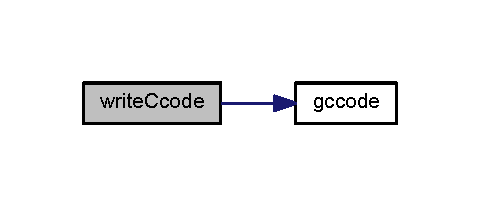
\includegraphics[width=230pt]{classamifun_a8e48f2842268ff64ca32db8eb4b69377_cgraph}
\end{center}
\end{figure}
\mbox{\Hypertarget{classamifun_a9b041ce0ffcfab125b5db3ed5ca847a2}\label{classamifun_a9b041ce0ffcfab125b5db3ed5ca847a2}} 
\index{amifun@{amifun}!writeMcode@{writeMcode}}
\index{writeMcode@{writeMcode}!amifun@{amifun}}
\doxyparagraph{\texorpdfstring{writeMcode()}{writeMcode()}}
{\footnotesize\ttfamily noret\+::substitute write\+Mcode (\begin{DoxyParamCaption}\item[{\+::\mbox{\hyperlink{classamimodel}{amimodel}}}]{model }\end{DoxyParamCaption})}


\begin{DoxyParams}{Parameters}
{\em model} & model defintion object\\
\hline
\end{DoxyParams}

\begin{DoxyRetVals}{Return values}
{\em model} & void \\
\hline
\end{DoxyRetVals}


Definition at line 18 of file write\+Mcode.\+m.

Here is the call graph for this function\+:
\nopagebreak
\begin{figure}[H]
\begin{center}
\leavevmode
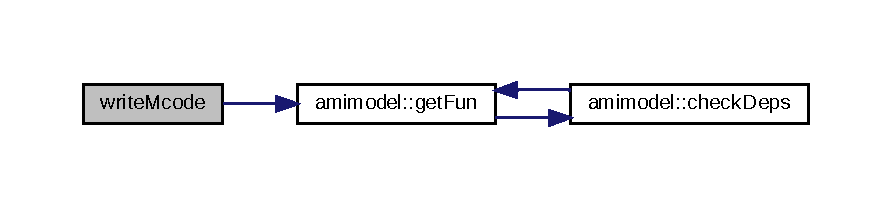
\includegraphics[width=350pt]{classamifun_a9b041ce0ffcfab125b5db3ed5ca847a2_cgraph}
\end{center}
\end{figure}
\mbox{\Hypertarget{classamifun_a05444f498e657a0010f6b539bc9c6596}\label{classamifun_a05444f498e657a0010f6b539bc9c6596}} 
\index{amifun@{amifun}!gccode@{gccode}}
\index{gccode@{gccode}!amifun@{amifun}}
\doxyparagraph{\texorpdfstring{gccode()}{gccode()}}
{\footnotesize\ttfamily mlhs\+Inner\+Subst$<$\+::\mbox{\hyperlink{classamifun}{amifun}} $>$ gccode (\begin{DoxyParamCaption}\item[{\+::\mbox{\hyperlink{classamimodel}{amimodel}}}]{model,  }\item[{\+::fileid}]{fid }\end{DoxyParamCaption})}


\begin{DoxyParams}{Parameters}
{\em model} & model definition object \\
\hline
{\em fid} & file id in which the expression should be written\\
\hline
\end{DoxyParams}

\begin{DoxyRetVals}{Return values}
{\em this} & function definition object \\
\hline
\end{DoxyRetVals}


Definition at line 18 of file gccode.\+m.

Here is the caller graph for this function\+:
\nopagebreak
\begin{figure}[H]
\begin{center}
\leavevmode
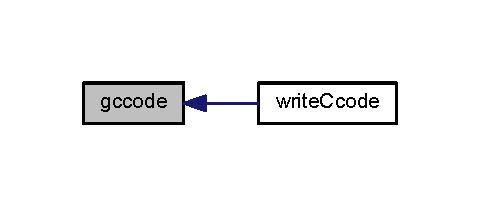
\includegraphics[width=230pt]{classamifun_a05444f498e657a0010f6b539bc9c6596_icgraph}
\end{center}
\end{figure}
\mbox{\Hypertarget{classamifun_a1cb97b695ab609e1655ec1067b140b70}\label{classamifun_a1cb97b695ab609e1655ec1067b140b70}} 
\index{amifun@{amifun}!getDeps@{getDeps}}
\index{getDeps@{getDeps}!amifun@{amifun}}
\doxyparagraph{\texorpdfstring{getDeps()}{getDeps()}}
{\footnotesize\ttfamily mlhs\+Inner\+Subst$<$\+::\mbox{\hyperlink{classamifun}{amifun}} $>$ get\+Deps (\begin{DoxyParamCaption}\item[{\+::\mbox{\hyperlink{classamimodel}{amimodel}}}]{model }\end{DoxyParamCaption})}


\begin{DoxyParams}{Parameters}
{\em model} & model definition object\\
\hline
\end{DoxyParams}

\begin{DoxyRetVals}{Return values}
{\em this} & updated function definition object \\
\hline
\end{DoxyRetVals}


Definition at line 18 of file get\+Deps.\+m.

\mbox{\Hypertarget{classamifun_a4b16e7670c0d60e530545e58628bde3f}\label{classamifun_a4b16e7670c0d60e530545e58628bde3f}} 
\index{amifun@{amifun}!getArgs@{getArgs}}
\index{getArgs@{getArgs}!amifun@{amifun}}
\doxyparagraph{\texorpdfstring{getArgs()}{getArgs()}}
{\footnotesize\ttfamily mlhs\+Inner\+Subst$<$\+::\mbox{\hyperlink{classamifun}{amifun}} $>$ get\+Args (\begin{DoxyParamCaption}\item[{\+::\mbox{\hyperlink{classamimodel}{amimodel}}}]{model }\end{DoxyParamCaption})}


\begin{DoxyParams}{Parameters}
{\em model} & model definition object\\
\hline
\end{DoxyParams}

\begin{DoxyRetVals}{Return values}
{\em this} & updated function definition object \\
\hline
\end{DoxyRetVals}


Definition at line 18 of file get\+Args.\+m.

\mbox{\Hypertarget{classamifun_a3ae210044df5eb51e2f9280d03b86c3c}\label{classamifun_a3ae210044df5eb51e2f9280d03b86c3c}} 
\index{amifun@{amifun}!getNVecs@{getNVecs}}
\index{getNVecs@{getNVecs}!amifun@{amifun}}
\doxyparagraph{\texorpdfstring{getNVecs()}{getNVecs()}}
{\footnotesize\ttfamily mlhs\+Inner\+Subst$<$\+::\mbox{\hyperlink{classamifun}{amifun}} $>$ get\+N\+Vecs (\begin{DoxyParamCaption}{ }\end{DoxyParamCaption})}


\begin{DoxyRetVals}{Return values}
{\em this} & updated function definition object \\
\hline
\end{DoxyRetVals}


Definition at line 18 of file get\+N\+Vecs.\+m.

\mbox{\Hypertarget{classamifun_a969775839d9d32ff4a0ba70395117ca7}\label{classamifun_a969775839d9d32ff4a0ba70395117ca7}} 
\index{amifun@{amifun}!getCVar@{getCVar}}
\index{getCVar@{getCVar}!amifun@{amifun}}
\doxyparagraph{\texorpdfstring{getCVar()}{getCVar()}}
{\footnotesize\ttfamily mlhs\+Inner\+Subst$<$\+::\mbox{\hyperlink{classamifun}{amifun}} $>$ get\+C\+Var (\begin{DoxyParamCaption}{ }\end{DoxyParamCaption})}


\begin{DoxyRetVals}{Return values}
{\em this} & updated function definition object \\
\hline
\end{DoxyRetVals}


Definition at line 18 of file get\+C\+Var.\+m.

\mbox{\Hypertarget{classamifun_ac60147b051aa541057d0da18a78582a8}\label{classamifun_ac60147b051aa541057d0da18a78582a8}} 
\index{amifun@{amifun}!getSensiFlag@{getSensiFlag}}
\index{getSensiFlag@{getSensiFlag}!amifun@{amifun}}
\doxyparagraph{\texorpdfstring{getSensiFlag()}{getSensiFlag()}}
{\footnotesize\ttfamily mlhs\+Inner\+Subst$<$\+::\mbox{\hyperlink{classamifun}{amifun}} $>$ get\+Sensi\+Flag (\begin{DoxyParamCaption}{ }\end{DoxyParamCaption})}


\begin{DoxyRetVals}{Return values}
{\em this} & updated function definition object \\
\hline
\end{DoxyRetVals}


Definition at line 18 of file get\+Sensi\+Flag.\+m.

\mbox{\Hypertarget{classamifun_a44e49602645d85f94841f38e4673fa1a}\label{classamifun_a44e49602645d85f94841f38e4673fa1a}} 
\index{amifun@{amifun}!getSyms@{getSyms}}
\index{getSyms@{getSyms}!amifun@{amifun}}
\doxyparagraph{\texorpdfstring{getSyms()}{getSyms()}}
{\footnotesize\ttfamily mlhs\+Subst$<$ mlhs\+Inner\+Subst$<$\+::\mbox{\hyperlink{classamifun}{amifun}} $>$,mlhs\+Inner\+Subst$<$\+::\mbox{\hyperlink{classamimodel}{amimodel}} $>$ $>$ get\+Syms (\begin{DoxyParamCaption}\item[{\+::\mbox{\hyperlink{classamimodel}{amimodel}}}]{model }\end{DoxyParamCaption})}


\begin{DoxyParams}{Parameters}
{\em model} & model definition object\\
\hline
\end{DoxyParams}

\begin{DoxyRetVals}{Return values}
{\em this} & updated function definition object \\
\hline
{\em model} & updated model definition object \\
\hline
\end{DoxyRetVals}


Definition at line 18 of file get\+Syms.\+m.

Here is the call graph for this function\+:
\nopagebreak
\begin{figure}[H]
\begin{center}
\leavevmode
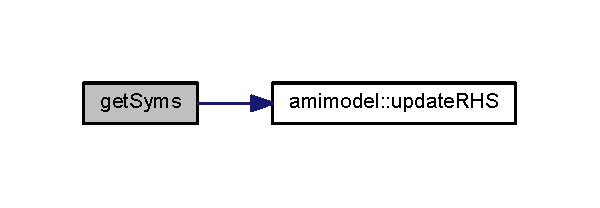
\includegraphics[width=288pt]{classamifun_a44e49602645d85f94841f38e4673fa1a_cgraph}
\end{center}
\end{figure}


\doxysubsubsection{Member Data Documentation}
\mbox{\Hypertarget{classamifun_a3c48fff3d28406486a4f1b5e18da7ca6}\label{classamifun_a3c48fff3d28406486a4f1b5e18da7ca6}} 
\index{amifun@{amifun}!sym@{sym}}
\index{sym@{sym}!amifun@{amifun}}
\doxyparagraph{\texorpdfstring{sym}{sym}}
{\footnotesize\ttfamily sym = sym(\char`\"{}\mbox{[}$\,$\mbox{]}\char`\"{})}

~\newline
{\bfseries{Default\+:}} sym(\char`\"{}\mbox{[}$\,$\mbox{]}\char`\"{}) 

Definition at line 27 of file amifun.\+m.

\mbox{\Hypertarget{classamifun_a653c7ed7ae2eeb18b7cb2f0a6be8ab5b}\label{classamifun_a653c7ed7ae2eeb18b7cb2f0a6be8ab5b}} 
\index{amifun@{amifun}!sym\_noopt@{sym\_noopt}}
\index{sym\_noopt@{sym\_noopt}!amifun@{amifun}}
\doxyparagraph{\texorpdfstring{sym\_noopt}{sym\_noopt}}
{\footnotesize\ttfamily sym\+\_\+noopt = \mbox{\hyperlink{classamifun_a3c48fff3d28406486a4f1b5e18da7ca6}{sym}}(\char`\"{}\mbox{[}$\,$\mbox{]}\char`\"{})}

~\newline
{\bfseries{Default\+:}} sym(\char`\"{}\mbox{[}$\,$\mbox{]}\char`\"{}) 

Definition at line 35 of file amifun.\+m.

\mbox{\Hypertarget{classamifun_a4814315a739f43461b003c1c1ef6f550}\label{classamifun_a4814315a739f43461b003c1c1ef6f550}} 
\index{amifun@{amifun}!strsym@{strsym}}
\index{strsym@{strsym}!amifun@{amifun}}
\doxyparagraph{\texorpdfstring{strsym}{strsym}}
{\footnotesize\ttfamily strsym = \mbox{\hyperlink{classamifun_a3c48fff3d28406486a4f1b5e18da7ca6}{sym}}(\char`\"{}\mbox{[}$\,$\mbox{]}\char`\"{})}

~\newline
{\bfseries{Default\+:}} sym(\char`\"{}\mbox{[}$\,$\mbox{]}\char`\"{}) 

Definition at line 43 of file amifun.\+m.

\mbox{\Hypertarget{classamifun_ac42759baa6575c9d39f487be5a2e01a1}\label{classamifun_ac42759baa6575c9d39f487be5a2e01a1}} 
\index{amifun@{amifun}!strsym\_old@{strsym\_old}}
\index{strsym\_old@{strsym\_old}!amifun@{amifun}}
\doxyparagraph{\texorpdfstring{strsym\_old}{strsym\_old}}
{\footnotesize\ttfamily strsym\+\_\+old = \mbox{\hyperlink{classamifun_a3c48fff3d28406486a4f1b5e18da7ca6}{sym}}(\char`\"{}\mbox{[}$\,$\mbox{]}\char`\"{})}

~\newline
{\bfseries{Default\+:}} sym(\char`\"{}\mbox{[}$\,$\mbox{]}\char`\"{}) 

Definition at line 51 of file amifun.\+m.

\mbox{\Hypertarget{classamifun_a484b54379bc8b29b6ce65d84966ea4c4}\label{classamifun_a484b54379bc8b29b6ce65d84966ea4c4}} 
\index{amifun@{amifun}!funstr@{funstr}}
\index{funstr@{funstr}!amifun@{amifun}}
\doxyparagraph{\texorpdfstring{funstr}{funstr}}
{\footnotesize\ttfamily funstr = char.\+empty(\char`\"{}\char`\"{})}

~\newline
{\bfseries{Default\+:}} char.\+empty(\char`\"{}\char`\"{}) 

Definition at line 59 of file amifun.\+m.

\mbox{\Hypertarget{classamifun_a716c1ceb8235bc1005b606f777530ede}\label{classamifun_a716c1ceb8235bc1005b606f777530ede}} 
\index{amifun@{amifun}!cvar@{cvar}}
\index{cvar@{cvar}!amifun@{amifun}}
\doxyparagraph{\texorpdfstring{cvar}{cvar}}
{\footnotesize\ttfamily cvar = char.\+empty(\char`\"{}\char`\"{})}

~\newline
{\bfseries{Default\+:}} char.\+empty(\char`\"{}\char`\"{}) 

Definition at line 67 of file amifun.\+m.

\mbox{\Hypertarget{classamifun_aa3914760f4131288b95f0f23d0fdfa6d}\label{classamifun_aa3914760f4131288b95f0f23d0fdfa6d}} 
\index{amifun@{amifun}!argstr@{argstr}}
\index{argstr@{argstr}!amifun@{amifun}}
\doxyparagraph{\texorpdfstring{argstr}{argstr}}
{\footnotesize\ttfamily argstr = char.\+empty(\char`\"{}\char`\"{})}

~\newline
{\bfseries{Default\+:}} char.\+empty(\char`\"{}\char`\"{}) 

Definition at line 75 of file amifun.\+m.

\mbox{\Hypertarget{classamifun_a69ffe5c24686ceb79ed44399e6be556c}\label{classamifun_a69ffe5c24686ceb79ed44399e6be556c}} 
\index{amifun@{amifun}!deps@{deps}}
\index{deps@{deps}!amifun@{amifun}}
\doxyparagraph{\texorpdfstring{deps}{deps}}
{\footnotesize\ttfamily deps = cell.\+empty(\char`\"{}\char`\"{})}

~\newline
{\bfseries{Default\+:}} cell.\+empty(\char`\"{}\char`\"{}) 

Definition at line 83 of file amifun.\+m.

\mbox{\Hypertarget{classamifun_a019d960f3d1c1c819a7f3fc90f952c4b}\label{classamifun_a019d960f3d1c1c819a7f3fc90f952c4b}} 
\index{amifun@{amifun}!nvecs@{nvecs}}
\index{nvecs@{nvecs}!amifun@{amifun}}
\doxyparagraph{\texorpdfstring{nvecs}{nvecs}}
{\footnotesize\ttfamily nvecs = cell.\+empty(\char`\"{}\char`\"{})}

~\newline
{\bfseries{Default\+:}} cell.\+empty(\char`\"{}\char`\"{}) 

Definition at line 91 of file amifun.\+m.

\mbox{\Hypertarget{classamifun_ad8930a02bca1d5facc6203b722d5349d}\label{classamifun_ad8930a02bca1d5facc6203b722d5349d}} 
\index{amifun@{amifun}!sensiflag@{sensiflag}}
\index{sensiflag@{sensiflag}!amifun@{amifun}}
\doxyparagraph{\texorpdfstring{sensiflag}{sensiflag}}
{\footnotesize\ttfamily sensiflag = logical.\+empty(\char`\"{}\char`\"{})}

~\newline
{\bfseries{Default\+:}} logical.\+empty(\char`\"{}\char`\"{}) 

Definition at line 99 of file amifun.\+m.


\hypertarget{classamimodel}{}\subsection{amimodel Class Reference}
\label{classamimodel}\index{amimodel@{amimodel}}


amimodel is the object in which all model definitions are stored  




Collaboration diagram for amimodel\+:\nopagebreak
\begin{figure}[H]
\begin{center}
\leavevmode
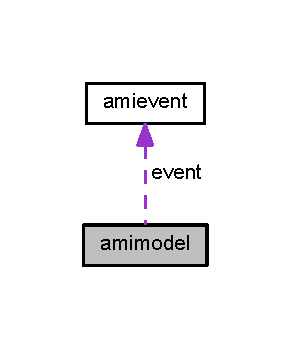
\includegraphics[width=139pt]{classamimodel__coll__graph}
\end{center}
\end{figure}
\subsubsection*{Public Member Functions}
\begin{DoxyCompactItemize}
\item 
\hyperlink{classamimodel_a05d52506788717b3d482845748446a60}{amimodel} (\+::string symfun,\+::string \hyperlink{classamimodel_a71bca9c21a6de42d8079ade31cb61044}{modelname})
\begin{DoxyCompactList}\small\item\em constructor of the amimodel class. this function initializes the model object based on the provided symfun and modelname \end{DoxyCompactList}\item 
mlhs\+Inner\+Subst$<$ matlabtypesubstitute $>$ \hyperlink{classamimodel_a68efdc6ed5d618672bea1556209e5568}{parse\+Model} ()
\begin{DoxyCompactList}\small\item\em parse\+Model parses the model definition and computes all necessary symbolic expressions. \end{DoxyCompactList}\item 
mlhs\+Inner\+Subst$<$ matlabtypesubstitute $>$ \hyperlink{classamimodel_af2ce5001c2320c95471ecb8c3d73bdbb}{generate\+C} ()
\begin{DoxyCompactList}\small\item\em generate\+C generates the c files which will be used in the compilation. \end{DoxyCompactList}\item 
mlhs\+Inner\+Subst$<$ matlabtypesubstitute $>$ \hyperlink{classamimodel_ad1339463ebc3a2e6c6aeda6f63f1b4ed}{compile\+C} ()
\begin{DoxyCompactList}\small\item\em compile\+C compiles the mex simulation file \end{DoxyCompactList}\item 
mlhs\+Inner\+Subst$<$ matlabtypesubstitute $>$ \hyperlink{classamimodel_a1b75344ed773e2c5c1b76b8a97861234}{generate\+M} (\+::\hyperlink{classamimodel}{amimodel} amimodelo2)
\begin{DoxyCompactList}\small\item\em generate\+M generates the matlab wrapper for the compiled C files. \end{DoxyCompactList}\item 
mlhs\+Inner\+Subst$<$ matlabtypesubstitute $>$ \hyperlink{classamimodel_a73f1b1b08350475e8d854d1a7f1944e1}{get\+Fun} (\+::struct \hyperlink{classamimodel_aafe6335df413dd688a2f44efba012cf1}{H\+Table},\+::string funstr)
\begin{DoxyCompactList}\small\item\em get\+Fun generates symbolic expressions for the requested function. \end{DoxyCompactList}\item 
mlhs\+Inner\+Subst$<$ matlabtypesubstitute $>$ \hyperlink{classamimodel_a2728abfdded1f9cd0d956118c7d32005}{make\+Events} ()
\begin{DoxyCompactList}\small\item\em make\+Events extracts discontiniuties from the model right hand side and converts them into events \end{DoxyCompactList}\item 
mlhs\+Inner\+Subst$<$ matlabtypesubstitute $>$ \hyperlink{classamimodel_a9f914e11f88fbdea879c0d8f4c26cd0a}{make\+Syms} ()
\begin{DoxyCompactList}\small\item\em make\+Syms extracts symbolic definition from the user provided model and checks them for consistency \end{DoxyCompactList}\item 
mlhs\+Subst$<$ mlhs\+Inner\+Subst$<$ matlabtypesubstitute $>$,mlhs\+Inner\+Subst$<$ matlabtypesubstitute $>$ $>$ \hyperlink{classamimodel_aa04dcfc1d2188cae948a75ebd46a6e03}{check\+Deps} (\+::struct \hyperlink{classamimodel_aafe6335df413dd688a2f44efba012cf1}{H\+Table},\+::cell deps)
\begin{DoxyCompactList}\small\item\em check\+Deps checks the dependencies of functions and populates sym fields if necessary \end{DoxyCompactList}\item 
mlhs\+Subst$<$ mlhs\+Inner\+Subst$<$ matlabtypesubstitute $>$,mlhs\+Inner\+Subst$<$ matlabtypesubstitute $>$ $>$ \hyperlink{classamimodel_ab21f46296b0ee0a141c38143a79ad396}{load\+Old\+Hashes} ()
\begin{DoxyCompactList}\small\item\em load\+Old\+Hashes loads information from a previous compilation of the model. \end{DoxyCompactList}\item 
mlhs\+Inner\+Subst$<$ matlabtypesubstitute $>$ \hyperlink{classamimodel_a2c41ab7adc2f815030ba175132e648c5}{augmento2} ()
\begin{DoxyCompactList}\small\item\em augmento2 augments the system equation to also include equations for sensitivity equation. This will enable us to compute second order sensitivities in a forward-\/adjoint or forward-\/forward apporach later on. \end{DoxyCompactList}\end{DoxyCompactItemize}
\subsubsection*{Public Attributes}
\begin{DoxyCompactItemize}
\item 
\+::struct \hyperlink{classamimodel_a3c48fff3d28406486a4f1b5e18da7ca6}{sym}
\begin{DoxyCompactList}\small\item\em symbolic definition struct \end{DoxyCompactList}\item 
\+::struct \hyperlink{classamimodel_a743fa290dbc0a67a3843d5ab0426e9b4}{fun}
\begin{DoxyCompactList}\small\item\em struct which stores information for which functions c code needs to be generated \end{DoxyCompactList}\item 
\+::$\ast$\hyperlink{classamievent}{amievent} \hyperlink{classamimodel_a3b65133bb9997cd1ccf311af0927fc9e}{event}
\begin{DoxyCompactList}\small\item\em struct which stores information for which functions c code needs to be generated \end{DoxyCompactList}\item 
\+::string \hyperlink{classamimodel_a71bca9c21a6de42d8079ade31cb61044}{modelname}
\begin{DoxyCompactList}\small\item\em name of the model \end{DoxyCompactList}\item 
\+::struct \hyperlink{classamimodel_aafe6335df413dd688a2f44efba012cf1}{H\+Table}
\begin{DoxyCompactList}\small\item\em struct that contains hash values for the symbolic model definitions \end{DoxyCompactList}\item 
\+::double \hyperlink{classamimodel_a0c5f3dcf809a17b895fe12fc91272349}{atol} = 1e-\/8
\begin{DoxyCompactList}\small\item\em default absolute tolerance \end{DoxyCompactList}\item 
\+::double \hyperlink{classamimodel_a7978e9a4674f869e6b2950e2f6262ca5}{rtol} = 1e-\/8
\begin{DoxyCompactList}\small\item\em default relative tolerance \end{DoxyCompactList}\item 
\+::int \hyperlink{classamimodel_ac37622882dacee1f11688d4941ccb45e}{maxsteps} = 1e4
\begin{DoxyCompactList}\small\item\em default maximal number of integration steps \end{DoxyCompactList}\item 
\+::bool \hyperlink{classamimodel_a0514aabed091ee5e2f35766eb01eced6}{debug} = false
\begin{DoxyCompactList}\small\item\em flag indicating whether debugging symbols should be compiled \end{DoxyCompactList}\item 
\+::bool \hyperlink{classamimodel_ab6d500b41cf50693452415caca31d32e}{adjoint} = true
\begin{DoxyCompactList}\small\item\em flag indicating whether adjoint sensitivities should be enabled \end{DoxyCompactList}\item 
\+::bool \hyperlink{classamimodel_a81e42e48c9c72814166c8f7cd414ce24}{forward} = true
\begin{DoxyCompactList}\small\item\em flag indicating whether forward sensitivities should be enabled \end{DoxyCompactList}\item 
\+::double \hyperlink{classamimodel_abdb5a42ffee3ca622484b53a322f1004}{t0} = 0
\begin{DoxyCompactList}\small\item\em default initial time \end{DoxyCompactList}\item 
\+::string \hyperlink{classamimodel_a5376250224ce32fb558d88aa0b5a93ff}{wtype}
\begin{DoxyCompactList}\small\item\em type of wrapper (cvodes/idas) \end{DoxyCompactList}\item 
\+::int \hyperlink{classamimodel_a84e4236f07668a770c27567f1f9615ff}{nx}
\begin{DoxyCompactList}\small\item\em number of states \end{DoxyCompactList}\item 
\+::int \hyperlink{classamimodel_a49c476de14a021114feb8c95da04952a}{nxtrue} = 0
\begin{DoxyCompactList}\small\item\em number of original states for second order sensitivities \end{DoxyCompactList}\item 
\+::int \hyperlink{classamimodel_a289ca425eb368f1d582b6be2be0d3dfc}{ny}
\begin{DoxyCompactList}\small\item\em number of observables \end{DoxyCompactList}\item 
\+::int \hyperlink{classamimodel_ac91d7b36031ec122abc9f739692b02e8}{nytrue} = 0
\begin{DoxyCompactList}\small\item\em number of original observables for second order sensitivities \end{DoxyCompactList}\item 
\+::int \hyperlink{classamimodel_a6f6e2fe71b05c4c2f2d967ce9ca02dfd}{np}
\begin{DoxyCompactList}\small\item\em number of parameters \end{DoxyCompactList}\item 
\+::int \hyperlink{classamimodel_afd6bea572754e0c3c320664bdccf0200}{nk}
\begin{DoxyCompactList}\small\item\em number of constants \end{DoxyCompactList}\item 
\+::int \hyperlink{classamimodel_aab5c7f06273122b68624eb3bca6a9b6e}{nevent}
\begin{DoxyCompactList}\small\item\em number of events \end{DoxyCompactList}\item 
\+::int \hyperlink{classamimodel_a79f11413e5bfe18a0e71e17574399ad5}{nz}
\begin{DoxyCompactList}\small\item\em number of event outputs \end{DoxyCompactList}\item 
\+::$\ast$int \hyperlink{classamimodel_acf2488b95c97e0378c9bf49de3b50f28}{id}
\begin{DoxyCompactList}\small\item\em flag for D\+A\+Es \end{DoxyCompactList}\item 
\+::int \hyperlink{classamimodel_a955c9d10635afed4ebc04c60010e5d40}{ubw}
\begin{DoxyCompactList}\small\item\em upper Jacobian bandwidth \end{DoxyCompactList}\item 
\+::int \hyperlink{classamimodel_a784f5fb2b8eda576179be087c2a09a39}{lbw}
\begin{DoxyCompactList}\small\item\em lower Jacobian bandwidth \end{DoxyCompactList}\item 
\+::int \hyperlink{classamimodel_a825ec588729c090ff51ea3473dcbc6b9}{nnz}
\begin{DoxyCompactList}\small\item\em number of nonzero entries in Jacobian \end{DoxyCompactList}\item 
\+::$\ast$int \hyperlink{classamimodel_a6ffb112eda9ff756e17104210981b30b}{sparseidx}
\begin{DoxyCompactList}\small\item\em dataindexes of sparse Jacobian \end{DoxyCompactList}\item 
\+::$\ast$int \hyperlink{classamimodel_aa0abea3560da3f409a28567f42d52872}{rowvals}
\begin{DoxyCompactList}\small\item\em rowindexes of sparse Jacobian \end{DoxyCompactList}\item 
\+::$\ast$int \hyperlink{classamimodel_a887e8a11654afa197d040d8bb10cbb38}{colptrs}
\begin{DoxyCompactList}\small\item\em columnindexes of sparse Jacobian \end{DoxyCompactList}\item 
\+::$\ast$int \hyperlink{classamimodel_adcfae93a688a66f1954d0832f51e4cc0}{sparseidx\+B}
\begin{DoxyCompactList}\small\item\em dataindexes of sparse Jacobian \end{DoxyCompactList}\item 
\+::$\ast$int \hyperlink{classamimodel_a1ba81ee0e28fe7c7576911973c82be70}{rowvals\+B}
\begin{DoxyCompactList}\small\item\em rowindexes of sparse Jacobian \end{DoxyCompactList}\item 
\+::$\ast$int \hyperlink{classamimodel_a3a4891c5565b544dd7d4362dbbfaadf7}{colptrs\+B}
\begin{DoxyCompactList}\small\item\em columnindexes of sparse Jacobian \end{DoxyCompactList}\item 
\+::$\ast$cell \hyperlink{classamimodel_af80b2560853c3df2b09fef2a198cf5b8}{funs}
\begin{DoxyCompactList}\small\item\em cell array of functions to be compiled \end{DoxyCompactList}\item 
\+::string \hyperlink{classamimodel_ad99abcd270ac97546c46292ebc6c2e0a}{coptim} = \char`\"{}-\/O3\char`\"{}
\begin{DoxyCompactList}\small\item\em optimisation flag for compilation \end{DoxyCompactList}\item 
\+::string \hyperlink{classamimodel_a51f20d6b1b54a2eee3be0e8adc96a0ae}{param} = \char`\"{}lin\char`\"{}
\begin{DoxyCompactList}\small\item\em default parametrisation \end{DoxyCompactList}\item 
matlabtypesubstitute \hyperlink{classamimodel_a0b316a20054ba282555674d939a82406}{wrap\+\_\+path}
\begin{DoxyCompactList}\small\item\em path to wrapper \end{DoxyCompactList}\item 
matlabtypesubstitute \hyperlink{classamimodel_a8d2e824e03e32034b634a7c48f2a26c6}{recompile} = false
\begin{DoxyCompactList}\small\item\em flag to enforce recompilation of the model \end{DoxyCompactList}\item 
matlabtypesubstitute \hyperlink{classamimodel_afec809c626a350367485aa6aaea6b585}{cfun}
\begin{DoxyCompactList}\small\item\em storage for flags determining recompilation of individual functions \end{DoxyCompactList}\item 
matlabtypesubstitute \hyperlink{classamimodel_a0a9e4caf628a02e6db68e91c2de6f382}{compver} = 2
\begin{DoxyCompactList}\small\item\em counter that allows enforcing of recompilation of models after code changes \end{DoxyCompactList}\item 
\hypertarget{classamimodel_a7a7be015feeb7a346dceccd49e622b4b}{}matlabtypesubstitute \hyperlink{classamimodel_a7a7be015feeb7a346dceccd49e622b4b}{z2event}\label{classamimodel_a7a7be015feeb7a346dceccd49e622b4b}

\begin{DoxyCompactList}\small\item\em vector that maps outputs to events \end{DoxyCompactList}\end{DoxyCompactItemize}


\subsubsection{Detailed Description}


Definition at line 17 of file amimodel.\+m.



\subsubsection{Constructor \& Destructor Documentation}
\hypertarget{classamimodel_a05d52506788717b3d482845748446a60}{}\index{amimodel@{amimodel}!amimodel@{amimodel}}
\index{amimodel@{amimodel}!amimodel@{amimodel}}
\paragraph[{amimodel(\+::string symfun,\+::string modelname)}]{\setlength{\rightskip}{0pt plus 5cm}{\bf amimodel} (
\begin{DoxyParamCaption}
\item[{\+::string}]{symfun, }
\item[{\+::string}]{modelname}
\end{DoxyParamCaption}
)}\label{classamimodel_a05d52506788717b3d482845748446a60}

\begin{DoxyParams}{Parameters}
{\em symfun} & this is the string to the function which generates the modelstruct. You can also directly pass the struct here \\
\hline
{\em modelname} & name of the model \\
\hline
\end{DoxyParams}


Definition at line 435 of file amimodel.\+m.



\subsubsection{Member Function Documentation}
\hypertarget{classamimodel_a68efdc6ed5d618672bea1556209e5568}{}\index{amimodel@{amimodel}!parse\+Model@{parse\+Model}}
\index{parse\+Model@{parse\+Model}!amimodel@{amimodel}}
\paragraph[{parse\+Model()}]{\setlength{\rightskip}{0pt plus 5cm}mlhs\+Inner\+Subst$<$\+::{\bf amimodel} $>$ parse\+Model (
\begin{DoxyParamCaption}
{}
\end{DoxyParamCaption}
)}\label{classamimodel_a68efdc6ed5d618672bea1556209e5568}

\begin{DoxyRetVals}{Return values}
{\em this} & updated model definition object \\
\hline
\end{DoxyRetVals}


Definition at line 18 of file parse\+Model.\+m.



Here is the call graph for this function\+:\nopagebreak
\begin{figure}[H]
\begin{center}
\leavevmode
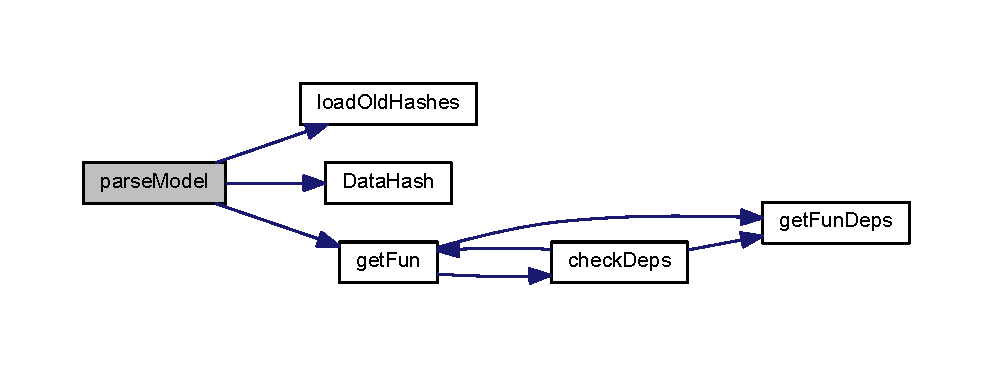
\includegraphics[width=350pt]{classamimodel_a68efdc6ed5d618672bea1556209e5568_cgraph}
\end{center}
\end{figure}


\hypertarget{classamimodel_af2ce5001c2320c95471ecb8c3d73bdbb}{}\index{amimodel@{amimodel}!generate\+C@{generate\+C}}
\index{generate\+C@{generate\+C}!amimodel@{amimodel}}
\paragraph[{generate\+C()}]{\setlength{\rightskip}{0pt plus 5cm}mlhs\+Inner\+Subst$<$\+::{\bf amimodel} $>$ generate\+C (
\begin{DoxyParamCaption}
{}
\end{DoxyParamCaption}
)}\label{classamimodel_af2ce5001c2320c95471ecb8c3d73bdbb}

\begin{DoxyRetVals}{Return values}
{\em this} & model definition object \\
\hline
\end{DoxyRetVals}


Definition at line 18 of file generate\+C.\+m.

\hypertarget{classamimodel_ad1339463ebc3a2e6c6aeda6f63f1b4ed}{}\index{amimodel@{amimodel}!compile\+C@{compile\+C}}
\index{compile\+C@{compile\+C}!amimodel@{amimodel}}
\paragraph[{compile\+C()}]{\setlength{\rightskip}{0pt plus 5cm}mlhs\+Inner\+Subst$<$\+::{\bf amimodel} $>$ compile\+C (
\begin{DoxyParamCaption}
{}
\end{DoxyParamCaption}
)}\label{classamimodel_ad1339463ebc3a2e6c6aeda6f63f1b4ed}

\begin{DoxyRetVals}{Return values}
{\em this} & model definition object \\
\hline
\end{DoxyRetVals}


Definition at line 18 of file compile\+C.\+m.

\hypertarget{classamimodel_a1b75344ed773e2c5c1b76b8a97861234}{}\index{amimodel@{amimodel}!generate\+M@{generate\+M}}
\index{generate\+M@{generate\+M}!amimodel@{amimodel}}
\paragraph[{generate\+M(\+::amimodel amimodelo2)}]{\setlength{\rightskip}{0pt plus 5cm}mlhs\+Inner\+Subst$<$\+::{\bf amimodel} $>$ generate\+M (
\begin{DoxyParamCaption}
\item[{\+::{\bf amimodel}}]{amimodelo2}
\end{DoxyParamCaption}
)}\label{classamimodel_a1b75344ed773e2c5c1b76b8a97861234}

\begin{DoxyParams}{Parameters}
{\em amimodelo2} & this struct must contain all necessary symbolic definitions for second order sensivities\\
\hline
\end{DoxyParams}

\begin{DoxyRetVals}{Return values}
{\em this} & model definition object \\
\hline
\end{DoxyRetVals}


Definition at line 18 of file generate\+M.\+m.

\hypertarget{classamimodel_a73f1b1b08350475e8d854d1a7f1944e1}{}\index{amimodel@{amimodel}!get\+Fun@{get\+Fun}}
\index{get\+Fun@{get\+Fun}!amimodel@{amimodel}}
\paragraph[{get\+Fun(\+::struct H\+Table,\+::string funstr)}]{\setlength{\rightskip}{0pt plus 5cm}mlhs\+Inner\+Subst$<$\+::{\bf amimodel} $>$ get\+Fun (
\begin{DoxyParamCaption}
\item[{\+::struct}]{H\+Table, }
\item[{\+::string}]{funstr}
\end{DoxyParamCaption}
)}\label{classamimodel_a73f1b1b08350475e8d854d1a7f1944e1}

\begin{DoxyParams}{Parameters}
{\em H\+Table} & struct with hashes of symbolic definition from the previous compilation \\
\hline
{\em funstr} & function for which symbolic expressions should be computed\\
\hline
\end{DoxyParams}

\begin{DoxyRetVals}{Return values}
{\em this} & updated model definition object \\
\hline
\end{DoxyRetVals}


Definition at line 18 of file get\+Fun.\+m.



Here is the call graph for this function\+:\nopagebreak
\begin{figure}[H]
\begin{center}
\leavevmode
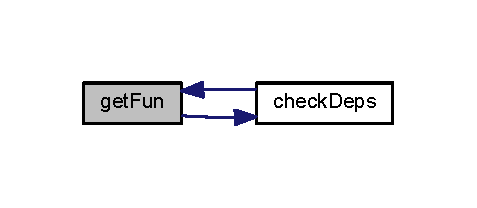
\includegraphics[width=229pt]{classamimodel_a73f1b1b08350475e8d854d1a7f1944e1_cgraph}
\end{center}
\end{figure}




Here is the caller graph for this function\+:\nopagebreak
\begin{figure}[H]
\begin{center}
\leavevmode
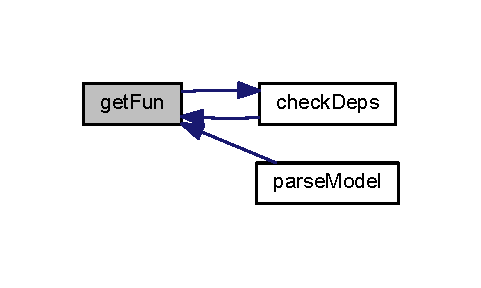
\includegraphics[width=231pt]{classamimodel_a73f1b1b08350475e8d854d1a7f1944e1_icgraph}
\end{center}
\end{figure}


\hypertarget{classamimodel_a2728abfdded1f9cd0d956118c7d32005}{}\index{amimodel@{amimodel}!make\+Events@{make\+Events}}
\index{make\+Events@{make\+Events}!amimodel@{amimodel}}
\paragraph[{make\+Events()}]{\setlength{\rightskip}{0pt plus 5cm}mlhs\+Inner\+Subst$<$\+::{\bf amimodel} $>$ make\+Events (
\begin{DoxyParamCaption}
{}
\end{DoxyParamCaption}
)}\label{classamimodel_a2728abfdded1f9cd0d956118c7d32005}

\begin{DoxyRetVals}{Return values}
{\em this} & updated model definition object \\
\hline
\end{DoxyRetVals}


Definition at line 18 of file make\+Events.\+m.

\hypertarget{classamimodel_a9f914e11f88fbdea879c0d8f4c26cd0a}{}\index{amimodel@{amimodel}!make\+Syms@{make\+Syms}}
\index{make\+Syms@{make\+Syms}!amimodel@{amimodel}}
\paragraph[{make\+Syms()}]{\setlength{\rightskip}{0pt plus 5cm}mlhs\+Inner\+Subst$<$\+::{\bf amimodel} $>$ make\+Syms (
\begin{DoxyParamCaption}
{}
\end{DoxyParamCaption}
)}\label{classamimodel_a9f914e11f88fbdea879c0d8f4c26cd0a}

\begin{DoxyRetVals}{Return values}
{\em this} & updated model definition object \\
\hline
\end{DoxyRetVals}


Definition at line 18 of file make\+Syms.\+m.

\hypertarget{classamimodel_aa04dcfc1d2188cae948a75ebd46a6e03}{}\index{amimodel@{amimodel}!check\+Deps@{check\+Deps}}
\index{check\+Deps@{check\+Deps}!amimodel@{amimodel}}
\paragraph[{check\+Deps(\+::struct H\+Table,\+::cell deps)}]{\setlength{\rightskip}{0pt plus 5cm}mlhs\+Subst$<$ mlhs\+Inner\+Subst$<$ matlabtypesubstitute $>$,mlhs\+Inner\+Subst$<$\+::{\bf H\+Table} $>$ $>$ check\+Deps (
\begin{DoxyParamCaption}
\item[{\+::struct}]{H\+Table, }
\item[{\+::cell}]{deps}
\end{DoxyParamCaption}
)}\label{classamimodel_aa04dcfc1d2188cae948a75ebd46a6e03}

\begin{DoxyParams}{Parameters}
{\em H\+Table} & struct with reference hashes of functions in its fields\\
\hline
{\em deps} & cell array with containing a list of dependencies\\
\hline
\end{DoxyParams}

\begin{DoxyRetVals}{Return values}
{\em cflag} & boolean indicating whether any of the dependencies have\\
\hline
\end{DoxyRetVals}
changed with respect to the hashes stored in H\+Table 

Definition at line 18 of file check\+Deps.\+m.



Here is the call graph for this function\+:\nopagebreak
\begin{figure}[H]
\begin{center}
\leavevmode
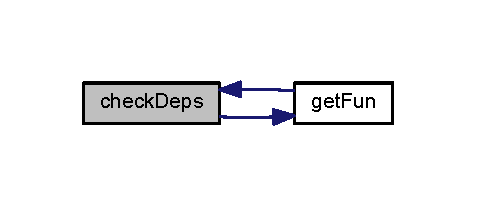
\includegraphics[width=229pt]{classamimodel_aa04dcfc1d2188cae948a75ebd46a6e03_cgraph}
\end{center}
\end{figure}




Here is the caller graph for this function\+:\nopagebreak
\begin{figure}[H]
\begin{center}
\leavevmode
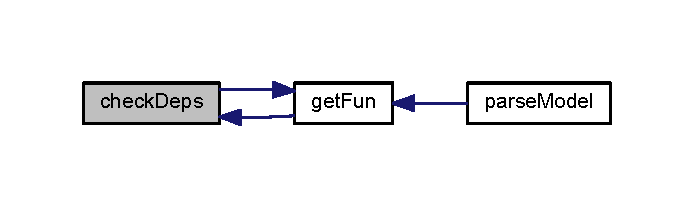
\includegraphics[width=333pt]{classamimodel_aa04dcfc1d2188cae948a75ebd46a6e03_icgraph}
\end{center}
\end{figure}


\hypertarget{classamimodel_ab21f46296b0ee0a141c38143a79ad396}{}\index{amimodel@{amimodel}!load\+Old\+Hashes@{load\+Old\+Hashes}}
\index{load\+Old\+Hashes@{load\+Old\+Hashes}!amimodel@{amimodel}}
\paragraph[{load\+Old\+Hashes()}]{\setlength{\rightskip}{0pt plus 5cm}mlhs\+Subst$<$ mlhs\+Inner\+Subst$<$\+::{\bf amimodel} $>$,mlhs\+Inner\+Subst$<$\+::struct $>$ $>$ load\+Old\+Hashes (
\begin{DoxyParamCaption}
{}
\end{DoxyParamCaption}
)}\label{classamimodel_ab21f46296b0ee0a141c38143a79ad396}

\begin{DoxyRetVals}{Return values}
{\em this} & updated model definition object \\
\hline
{\em H\+Table} & struct with hashes of symbolic definition from the previous compilation \\
\hline
\end{DoxyRetVals}


Definition at line 18 of file load\+Old\+Hashes.\+m.



Here is the caller graph for this function\+:\nopagebreak
\begin{figure}[H]
\begin{center}
\leavevmode
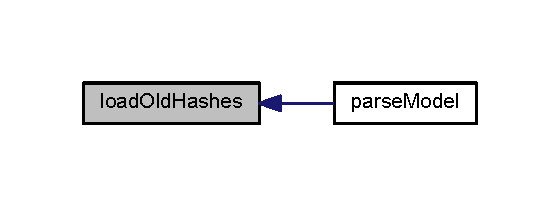
\includegraphics[width=269pt]{classamimodel_ab21f46296b0ee0a141c38143a79ad396_icgraph}
\end{center}
\end{figure}


\hypertarget{classamimodel_a2c41ab7adc2f815030ba175132e648c5}{}\index{amimodel@{amimodel}!augmento2@{augmento2}}
\index{augmento2@{augmento2}!amimodel@{amimodel}}
\paragraph[{augmento2()}]{\setlength{\rightskip}{0pt plus 5cm}mlhs\+Inner\+Subst$<$\+::{\bf amimodel} $>$ augmento2 (
\begin{DoxyParamCaption}
{}
\end{DoxyParamCaption}
)}\label{classamimodel_a2c41ab7adc2f815030ba175132e648c5}

\begin{DoxyRetVals}{Return values}
{\em this} & augmented system which contains symbolic definition of the original system and its sensitivities \\
\hline
\end{DoxyRetVals}


Definition at line 18 of file augmento2.\+m.



\subsubsection{Member Data Documentation}
\hypertarget{classamimodel_a3c48fff3d28406486a4f1b5e18da7ca6}{}\index{amimodel@{amimodel}!sym@{sym}}
\index{sym@{sym}!amimodel@{amimodel}}
\paragraph[{sym}]{\setlength{\rightskip}{0pt plus 5cm}sym}\label{classamimodel_a3c48fff3d28406486a4f1b5e18da7ca6}
\begin{DoxyNote}{Note}
This property has non-\/standard access specifiers\+: {\ttfamily Set\+Access = Private, Get\+Access = Public} 

\href{http://www.mathworks.com/help/matlab/matlab_oop/property-attributes.html}{\tt Matlab documentation of property attributes.} 
\end{DoxyNote}


Definition at line 26 of file amimodel.\+m.

\hypertarget{classamimodel_a743fa290dbc0a67a3843d5ab0426e9b4}{}\index{amimodel@{amimodel}!fun@{fun}}
\index{fun@{fun}!amimodel@{amimodel}}
\paragraph[{fun}]{\setlength{\rightskip}{0pt plus 5cm}fun}\label{classamimodel_a743fa290dbc0a67a3843d5ab0426e9b4}
\begin{DoxyNote}{Note}
This property has non-\/standard access specifiers\+: {\ttfamily Set\+Access = Private, Get\+Access = Public} 

\href{http://www.mathworks.com/help/matlab/matlab_oop/property-attributes.html}{\tt Matlab documentation of property attributes.} 
\end{DoxyNote}


Definition at line 36 of file amimodel.\+m.

\hypertarget{classamimodel_a3b65133bb9997cd1ccf311af0927fc9e}{}\index{amimodel@{amimodel}!event@{event}}
\index{event@{event}!amimodel@{amimodel}}
\paragraph[{event}]{\setlength{\rightskip}{0pt plus 5cm}event}\label{classamimodel_a3b65133bb9997cd1ccf311af0927fc9e}
\begin{DoxyNote}{Note}
This property has non-\/standard access specifiers\+: {\ttfamily Set\+Access = Private, Get\+Access = Public} 

\href{http://www.mathworks.com/help/matlab/matlab_oop/property-attributes.html}{\tt Matlab documentation of property attributes.} 
\end{DoxyNote}


Definition at line 46 of file amimodel.\+m.

\hypertarget{classamimodel_a71bca9c21a6de42d8079ade31cb61044}{}\index{amimodel@{amimodel}!modelname@{modelname}}
\index{modelname@{modelname}!amimodel@{amimodel}}
\paragraph[{modelname}]{\setlength{\rightskip}{0pt plus 5cm}modelname}\label{classamimodel_a71bca9c21a6de42d8079ade31cb61044}
\begin{DoxyNote}{Note}
This property has non-\/standard access specifiers\+: {\ttfamily Set\+Access = Private, Get\+Access = Public} 

\href{http://www.mathworks.com/help/matlab/matlab_oop/property-attributes.html}{\tt Matlab documentation of property attributes.} 
\end{DoxyNote}


Definition at line 57 of file amimodel.\+m.

\hypertarget{classamimodel_aafe6335df413dd688a2f44efba012cf1}{}\index{amimodel@{amimodel}!H\+Table@{H\+Table}}
\index{H\+Table@{H\+Table}!amimodel@{amimodel}}
\paragraph[{H\+Table}]{\setlength{\rightskip}{0pt plus 5cm}H\+Table}\label{classamimodel_aafe6335df413dd688a2f44efba012cf1}
\begin{DoxyNote}{Note}
This property has non-\/standard access specifiers\+: {\ttfamily Set\+Access = Private, Get\+Access = Public} 

\href{http://www.mathworks.com/help/matlab/matlab_oop/property-attributes.html}{\tt Matlab documentation of property attributes.} 
\end{DoxyNote}


Definition at line 67 of file amimodel.\+m.

\hypertarget{classamimodel_a0c5f3dcf809a17b895fe12fc91272349}{}\index{amimodel@{amimodel}!atol@{atol}}
\index{atol@{atol}!amimodel@{amimodel}}
\paragraph[{atol}]{\setlength{\rightskip}{0pt plus 5cm}atol = 1e-\/8}\label{classamimodel_a0c5f3dcf809a17b895fe12fc91272349}
\begin{DoxyNote}{Note}
This property has non-\/standard access specifiers\+: {\ttfamily Set\+Access = Private, Get\+Access = Public} 

\href{http://www.mathworks.com/help/matlab/matlab_oop/property-attributes.html}{\tt Matlab documentation of property attributes.} ~\newline
{\bfseries Default\+:} 1e-\/8 
\end{DoxyNote}


Definition at line 77 of file amimodel.\+m.

\hypertarget{classamimodel_a7978e9a4674f869e6b2950e2f6262ca5}{}\index{amimodel@{amimodel}!rtol@{rtol}}
\index{rtol@{rtol}!amimodel@{amimodel}}
\paragraph[{rtol}]{\setlength{\rightskip}{0pt plus 5cm}rtol = 1e-\/8}\label{classamimodel_a7978e9a4674f869e6b2950e2f6262ca5}
\begin{DoxyNote}{Note}
This property has non-\/standard access specifiers\+: {\ttfamily Set\+Access = Private, Get\+Access = Public} 

\href{http://www.mathworks.com/help/matlab/matlab_oop/property-attributes.html}{\tt Matlab documentation of property attributes.} ~\newline
{\bfseries Default\+:} 1e-\/8 
\end{DoxyNote}


Definition at line 88 of file amimodel.\+m.

\hypertarget{classamimodel_ac37622882dacee1f11688d4941ccb45e}{}\index{amimodel@{amimodel}!maxsteps@{maxsteps}}
\index{maxsteps@{maxsteps}!amimodel@{amimodel}}
\paragraph[{maxsteps}]{\setlength{\rightskip}{0pt plus 5cm}maxsteps = 1e4}\label{classamimodel_ac37622882dacee1f11688d4941ccb45e}
\begin{DoxyNote}{Note}
This property has non-\/standard access specifiers\+: {\ttfamily Set\+Access = Private, Get\+Access = Public} 

\href{http://www.mathworks.com/help/matlab/matlab_oop/property-attributes.html}{\tt Matlab documentation of property attributes.} ~\newline
{\bfseries Default\+:} 1e4 
\end{DoxyNote}


Definition at line 99 of file amimodel.\+m.

\hypertarget{classamimodel_a0514aabed091ee5e2f35766eb01eced6}{}\index{amimodel@{amimodel}!debug@{debug}}
\index{debug@{debug}!amimodel@{amimodel}}
\paragraph[{debug}]{\setlength{\rightskip}{0pt plus 5cm}debug = false}\label{classamimodel_a0514aabed091ee5e2f35766eb01eced6}
\begin{DoxyNote}{Note}
This property has non-\/standard access specifiers\+: {\ttfamily Set\+Access = Private, Get\+Access = Public} 

\href{http://www.mathworks.com/help/matlab/matlab_oop/property-attributes.html}{\tt Matlab documentation of property attributes.} ~\newline
{\bfseries Default\+:} false 
\end{DoxyNote}


Definition at line 110 of file amimodel.\+m.

\hypertarget{classamimodel_ab6d500b41cf50693452415caca31d32e}{}\index{amimodel@{amimodel}!adjoint@{adjoint}}
\index{adjoint@{adjoint}!amimodel@{amimodel}}
\paragraph[{adjoint}]{\setlength{\rightskip}{0pt plus 5cm}adjoint = true}\label{classamimodel_ab6d500b41cf50693452415caca31d32e}
\begin{DoxyNote}{Note}
This property has non-\/standard access specifiers\+: {\ttfamily Set\+Access = Private, Get\+Access = Public} 

\href{http://www.mathworks.com/help/matlab/matlab_oop/property-attributes.html}{\tt Matlab documentation of property attributes.} ~\newline
{\bfseries Default\+:} true 
\end{DoxyNote}


Definition at line 121 of file amimodel.\+m.

\hypertarget{classamimodel_a81e42e48c9c72814166c8f7cd414ce24}{}\index{amimodel@{amimodel}!forward@{forward}}
\index{forward@{forward}!amimodel@{amimodel}}
\paragraph[{forward}]{\setlength{\rightskip}{0pt plus 5cm}forward = true}\label{classamimodel_a81e42e48c9c72814166c8f7cd414ce24}
\begin{DoxyNote}{Note}
This property has non-\/standard access specifiers\+: {\ttfamily Set\+Access = Private, Get\+Access = Public} 

\href{http://www.mathworks.com/help/matlab/matlab_oop/property-attributes.html}{\tt Matlab documentation of property attributes.} ~\newline
{\bfseries Default\+:} true 
\end{DoxyNote}


Definition at line 132 of file amimodel.\+m.

\hypertarget{classamimodel_abdb5a42ffee3ca622484b53a322f1004}{}\index{amimodel@{amimodel}!t0@{t0}}
\index{t0@{t0}!amimodel@{amimodel}}
\paragraph[{t0}]{\setlength{\rightskip}{0pt plus 5cm}t0 = 0}\label{classamimodel_abdb5a42ffee3ca622484b53a322f1004}
\begin{DoxyNote}{Note}
This property has non-\/standard access specifiers\+: {\ttfamily Set\+Access = Private, Get\+Access = Public} 

\href{http://www.mathworks.com/help/matlab/matlab_oop/property-attributes.html}{\tt Matlab documentation of property attributes.} ~\newline
{\bfseries Default\+:} 0 
\end{DoxyNote}


Definition at line 143 of file amimodel.\+m.

\hypertarget{classamimodel_a5376250224ce32fb558d88aa0b5a93ff}{}\index{amimodel@{amimodel}!wtype@{wtype}}
\index{wtype@{wtype}!amimodel@{amimodel}}
\paragraph[{wtype}]{\setlength{\rightskip}{0pt plus 5cm}wtype}\label{classamimodel_a5376250224ce32fb558d88aa0b5a93ff}
\begin{DoxyNote}{Note}
This property has non-\/standard access specifiers\+: {\ttfamily Set\+Access = Private, Get\+Access = Public} 

\href{http://www.mathworks.com/help/matlab/matlab_oop/property-attributes.html}{\tt Matlab documentation of property attributes.} 
\end{DoxyNote}


Definition at line 154 of file amimodel.\+m.

\hypertarget{classamimodel_a84e4236f07668a770c27567f1f9615ff}{}\index{amimodel@{amimodel}!nx@{nx}}
\index{nx@{nx}!amimodel@{amimodel}}
\paragraph[{nx}]{\setlength{\rightskip}{0pt plus 5cm}nx}\label{classamimodel_a84e4236f07668a770c27567f1f9615ff}
\begin{DoxyNote}{Note}
This property has non-\/standard access specifiers\+: {\ttfamily Set\+Access = Private, Get\+Access = Public} 

\href{http://www.mathworks.com/help/matlab/matlab_oop/property-attributes.html}{\tt Matlab documentation of property attributes.} 
\end{DoxyNote}


Definition at line 164 of file amimodel.\+m.

\hypertarget{classamimodel_a49c476de14a021114feb8c95da04952a}{}\index{amimodel@{amimodel}!nxtrue@{nxtrue}}
\index{nxtrue@{nxtrue}!amimodel@{amimodel}}
\paragraph[{nxtrue}]{\setlength{\rightskip}{0pt plus 5cm}nxtrue = 0}\label{classamimodel_a49c476de14a021114feb8c95da04952a}
\begin{DoxyNote}{Note}
This property has non-\/standard access specifiers\+: {\ttfamily Set\+Access = Private, Get\+Access = Public} 

\href{http://www.mathworks.com/help/matlab/matlab_oop/property-attributes.html}{\tt Matlab documentation of property attributes.} ~\newline
{\bfseries Default\+:} 0 
\end{DoxyNote}


Definition at line 174 of file amimodel.\+m.

\hypertarget{classamimodel_a289ca425eb368f1d582b6be2be0d3dfc}{}\index{amimodel@{amimodel}!ny@{ny}}
\index{ny@{ny}!amimodel@{amimodel}}
\paragraph[{ny}]{\setlength{\rightskip}{0pt plus 5cm}ny}\label{classamimodel_a289ca425eb368f1d582b6be2be0d3dfc}
\begin{DoxyNote}{Note}
This property has non-\/standard access specifiers\+: {\ttfamily Set\+Access = Private, Get\+Access = Public} 

\href{http://www.mathworks.com/help/matlab/matlab_oop/property-attributes.html}{\tt Matlab documentation of property attributes.} 
\end{DoxyNote}


Definition at line 185 of file amimodel.\+m.

\hypertarget{classamimodel_ac91d7b36031ec122abc9f739692b02e8}{}\index{amimodel@{amimodel}!nytrue@{nytrue}}
\index{nytrue@{nytrue}!amimodel@{amimodel}}
\paragraph[{nytrue}]{\setlength{\rightskip}{0pt plus 5cm}nytrue = 0}\label{classamimodel_ac91d7b36031ec122abc9f739692b02e8}
\begin{DoxyNote}{Note}
This property has non-\/standard access specifiers\+: {\ttfamily Set\+Access = Private, Get\+Access = Public} 

\href{http://www.mathworks.com/help/matlab/matlab_oop/property-attributes.html}{\tt Matlab documentation of property attributes.} ~\newline
{\bfseries Default\+:} 0 
\end{DoxyNote}


Definition at line 195 of file amimodel.\+m.

\hypertarget{classamimodel_a6f6e2fe71b05c4c2f2d967ce9ca02dfd}{}\index{amimodel@{amimodel}!np@{np}}
\index{np@{np}!amimodel@{amimodel}}
\paragraph[{np}]{\setlength{\rightskip}{0pt plus 5cm}np}\label{classamimodel_a6f6e2fe71b05c4c2f2d967ce9ca02dfd}
\begin{DoxyNote}{Note}
This property has non-\/standard access specifiers\+: {\ttfamily Set\+Access = Private, Get\+Access = Public} 

\href{http://www.mathworks.com/help/matlab/matlab_oop/property-attributes.html}{\tt Matlab documentation of property attributes.} 
\end{DoxyNote}


Definition at line 206 of file amimodel.\+m.

\hypertarget{classamimodel_afd6bea572754e0c3c320664bdccf0200}{}\index{amimodel@{amimodel}!nk@{nk}}
\index{nk@{nk}!amimodel@{amimodel}}
\paragraph[{nk}]{\setlength{\rightskip}{0pt plus 5cm}nk}\label{classamimodel_afd6bea572754e0c3c320664bdccf0200}
\begin{DoxyNote}{Note}
This property has non-\/standard access specifiers\+: {\ttfamily Set\+Access = Private, Get\+Access = Public} 

\href{http://www.mathworks.com/help/matlab/matlab_oop/property-attributes.html}{\tt Matlab documentation of property attributes.} 
\end{DoxyNote}


Definition at line 216 of file amimodel.\+m.

\hypertarget{classamimodel_aab5c7f06273122b68624eb3bca6a9b6e}{}\index{amimodel@{amimodel}!nevent@{nevent}}
\index{nevent@{nevent}!amimodel@{amimodel}}
\paragraph[{nevent}]{\setlength{\rightskip}{0pt plus 5cm}nevent}\label{classamimodel_aab5c7f06273122b68624eb3bca6a9b6e}
\begin{DoxyNote}{Note}
This property has non-\/standard access specifiers\+: {\ttfamily Set\+Access = Private, Get\+Access = Public} 

\href{http://www.mathworks.com/help/matlab/matlab_oop/property-attributes.html}{\tt Matlab documentation of property attributes.} 
\end{DoxyNote}


Definition at line 226 of file amimodel.\+m.

\hypertarget{classamimodel_a79f11413e5bfe18a0e71e17574399ad5}{}\index{amimodel@{amimodel}!nz@{nz}}
\index{nz@{nz}!amimodel@{amimodel}}
\paragraph[{nz}]{\setlength{\rightskip}{0pt plus 5cm}nz}\label{classamimodel_a79f11413e5bfe18a0e71e17574399ad5}
\begin{DoxyNote}{Note}
This property has non-\/standard access specifiers\+: {\ttfamily Set\+Access = Private, Get\+Access = Public} 

\href{http://www.mathworks.com/help/matlab/matlab_oop/property-attributes.html}{\tt Matlab documentation of property attributes.} 
\end{DoxyNote}


Definition at line 236 of file amimodel.\+m.

\hypertarget{classamimodel_acf2488b95c97e0378c9bf49de3b50f28}{}\index{amimodel@{amimodel}!id@{id}}
\index{id@{id}!amimodel@{amimodel}}
\paragraph[{id}]{\setlength{\rightskip}{0pt plus 5cm}id}\label{classamimodel_acf2488b95c97e0378c9bf49de3b50f28}
\begin{DoxyNote}{Note}
This property has non-\/standard access specifiers\+: {\ttfamily Set\+Access = Private, Get\+Access = Public} 

\href{http://www.mathworks.com/help/matlab/matlab_oop/property-attributes.html}{\tt Matlab documentation of property attributes.} 
\end{DoxyNote}


Definition at line 246 of file amimodel.\+m.

\hypertarget{classamimodel_a955c9d10635afed4ebc04c60010e5d40}{}\index{amimodel@{amimodel}!ubw@{ubw}}
\index{ubw@{ubw}!amimodel@{amimodel}}
\paragraph[{ubw}]{\setlength{\rightskip}{0pt plus 5cm}ubw}\label{classamimodel_a955c9d10635afed4ebc04c60010e5d40}
\begin{DoxyNote}{Note}
This property has non-\/standard access specifiers\+: {\ttfamily Set\+Access = Private, Get\+Access = Public} 

\href{http://www.mathworks.com/help/matlab/matlab_oop/property-attributes.html}{\tt Matlab documentation of property attributes.} 
\end{DoxyNote}


Definition at line 256 of file amimodel.\+m.

\hypertarget{classamimodel_a784f5fb2b8eda576179be087c2a09a39}{}\index{amimodel@{amimodel}!lbw@{lbw}}
\index{lbw@{lbw}!amimodel@{amimodel}}
\paragraph[{lbw}]{\setlength{\rightskip}{0pt plus 5cm}lbw}\label{classamimodel_a784f5fb2b8eda576179be087c2a09a39}
\begin{DoxyNote}{Note}
This property has non-\/standard access specifiers\+: {\ttfamily Set\+Access = Private, Get\+Access = Public} 

\href{http://www.mathworks.com/help/matlab/matlab_oop/property-attributes.html}{\tt Matlab documentation of property attributes.} 
\end{DoxyNote}


Definition at line 266 of file amimodel.\+m.

\hypertarget{classamimodel_a825ec588729c090ff51ea3473dcbc6b9}{}\index{amimodel@{amimodel}!nnz@{nnz}}
\index{nnz@{nnz}!amimodel@{amimodel}}
\paragraph[{nnz}]{\setlength{\rightskip}{0pt plus 5cm}nnz}\label{classamimodel_a825ec588729c090ff51ea3473dcbc6b9}
\begin{DoxyNote}{Note}
This property has non-\/standard access specifiers\+: {\ttfamily Set\+Access = Private, Get\+Access = Public} 

\href{http://www.mathworks.com/help/matlab/matlab_oop/property-attributes.html}{\tt Matlab documentation of property attributes.} 
\end{DoxyNote}


Definition at line 276 of file amimodel.\+m.

\hypertarget{classamimodel_a6ffb112eda9ff756e17104210981b30b}{}\index{amimodel@{amimodel}!sparseidx@{sparseidx}}
\index{sparseidx@{sparseidx}!amimodel@{amimodel}}
\paragraph[{sparseidx}]{\setlength{\rightskip}{0pt plus 5cm}sparseidx}\label{classamimodel_a6ffb112eda9ff756e17104210981b30b}
\begin{DoxyNote}{Note}
This property has non-\/standard access specifiers\+: {\ttfamily Set\+Access = Private, Get\+Access = Public} 

\href{http://www.mathworks.com/help/matlab/matlab_oop/property-attributes.html}{\tt Matlab documentation of property attributes.} 
\end{DoxyNote}


Definition at line 286 of file amimodel.\+m.

\hypertarget{classamimodel_aa0abea3560da3f409a28567f42d52872}{}\index{amimodel@{amimodel}!rowvals@{rowvals}}
\index{rowvals@{rowvals}!amimodel@{amimodel}}
\paragraph[{rowvals}]{\setlength{\rightskip}{0pt plus 5cm}rowvals}\label{classamimodel_aa0abea3560da3f409a28567f42d52872}
\begin{DoxyNote}{Note}
This property has non-\/standard access specifiers\+: {\ttfamily Set\+Access = Private, Get\+Access = Public} 

\href{http://www.mathworks.com/help/matlab/matlab_oop/property-attributes.html}{\tt Matlab documentation of property attributes.} 
\end{DoxyNote}


Definition at line 296 of file amimodel.\+m.

\hypertarget{classamimodel_a887e8a11654afa197d040d8bb10cbb38}{}\index{amimodel@{amimodel}!colptrs@{colptrs}}
\index{colptrs@{colptrs}!amimodel@{amimodel}}
\paragraph[{colptrs}]{\setlength{\rightskip}{0pt plus 5cm}colptrs}\label{classamimodel_a887e8a11654afa197d040d8bb10cbb38}
\begin{DoxyNote}{Note}
This property has non-\/standard access specifiers\+: {\ttfamily Set\+Access = Private, Get\+Access = Public} 

\href{http://www.mathworks.com/help/matlab/matlab_oop/property-attributes.html}{\tt Matlab documentation of property attributes.} 
\end{DoxyNote}


Definition at line 306 of file amimodel.\+m.

\hypertarget{classamimodel_adcfae93a688a66f1954d0832f51e4cc0}{}\index{amimodel@{amimodel}!sparseidx\+B@{sparseidx\+B}}
\index{sparseidx\+B@{sparseidx\+B}!amimodel@{amimodel}}
\paragraph[{sparseidx\+B}]{\setlength{\rightskip}{0pt plus 5cm}sparseidx\+B}\label{classamimodel_adcfae93a688a66f1954d0832f51e4cc0}
\begin{DoxyNote}{Note}
This property has non-\/standard access specifiers\+: {\ttfamily Set\+Access = Private, Get\+Access = Public} 

\href{http://www.mathworks.com/help/matlab/matlab_oop/property-attributes.html}{\tt Matlab documentation of property attributes.} 
\end{DoxyNote}


Definition at line 316 of file amimodel.\+m.

\hypertarget{classamimodel_a1ba81ee0e28fe7c7576911973c82be70}{}\index{amimodel@{amimodel}!rowvals\+B@{rowvals\+B}}
\index{rowvals\+B@{rowvals\+B}!amimodel@{amimodel}}
\paragraph[{rowvals\+B}]{\setlength{\rightskip}{0pt plus 5cm}rowvals\+B}\label{classamimodel_a1ba81ee0e28fe7c7576911973c82be70}
\begin{DoxyNote}{Note}
This property has non-\/standard access specifiers\+: {\ttfamily Set\+Access = Private, Get\+Access = Public} 

\href{http://www.mathworks.com/help/matlab/matlab_oop/property-attributes.html}{\tt Matlab documentation of property attributes.} 
\end{DoxyNote}


Definition at line 326 of file amimodel.\+m.

\hypertarget{classamimodel_a3a4891c5565b544dd7d4362dbbfaadf7}{}\index{amimodel@{amimodel}!colptrs\+B@{colptrs\+B}}
\index{colptrs\+B@{colptrs\+B}!amimodel@{amimodel}}
\paragraph[{colptrs\+B}]{\setlength{\rightskip}{0pt plus 5cm}colptrs\+B}\label{classamimodel_a3a4891c5565b544dd7d4362dbbfaadf7}
\begin{DoxyNote}{Note}
This property has non-\/standard access specifiers\+: {\ttfamily Set\+Access = Private, Get\+Access = Public} 

\href{http://www.mathworks.com/help/matlab/matlab_oop/property-attributes.html}{\tt Matlab documentation of property attributes.} 
\end{DoxyNote}


Definition at line 336 of file amimodel.\+m.

\hypertarget{classamimodel_af80b2560853c3df2b09fef2a198cf5b8}{}\index{amimodel@{amimodel}!funs@{funs}}
\index{funs@{funs}!amimodel@{amimodel}}
\paragraph[{funs}]{\setlength{\rightskip}{0pt plus 5cm}funs}\label{classamimodel_af80b2560853c3df2b09fef2a198cf5b8}
\begin{DoxyNote}{Note}
This property has non-\/standard access specifiers\+: {\ttfamily Set\+Access = Private, Get\+Access = Public} 

\href{http://www.mathworks.com/help/matlab/matlab_oop/property-attributes.html}{\tt Matlab documentation of property attributes.} 
\end{DoxyNote}


Definition at line 346 of file amimodel.\+m.

\hypertarget{classamimodel_ad99abcd270ac97546c46292ebc6c2e0a}{}\index{amimodel@{amimodel}!coptim@{coptim}}
\index{coptim@{coptim}!amimodel@{amimodel}}
\paragraph[{coptim}]{\setlength{\rightskip}{0pt plus 5cm}coptim = \char`\"{}-\/O3\char`\"{}}\label{classamimodel_ad99abcd270ac97546c46292ebc6c2e0a}
\begin{DoxyNote}{Note}
This property has non-\/standard access specifiers\+: {\ttfamily Set\+Access = Private, Get\+Access = Public} 

\href{http://www.mathworks.com/help/matlab/matlab_oop/property-attributes.html}{\tt Matlab documentation of property attributes.} ~\newline
{\bfseries Default\+:} \char`\"{}-\/\+O3\char`\"{} 
\end{DoxyNote}


Definition at line 356 of file amimodel.\+m.

\hypertarget{classamimodel_a51f20d6b1b54a2eee3be0e8adc96a0ae}{}\index{amimodel@{amimodel}!param@{param}}
\index{param@{param}!amimodel@{amimodel}}
\paragraph[{param}]{\setlength{\rightskip}{0pt plus 5cm}param = \char`\"{}lin\char`\"{}}\label{classamimodel_a51f20d6b1b54a2eee3be0e8adc96a0ae}
\begin{DoxyNote}{Note}
This property has non-\/standard access specifiers\+: {\ttfamily Set\+Access = Private, Get\+Access = Public} 

\href{http://www.mathworks.com/help/matlab/matlab_oop/property-attributes.html}{\tt Matlab documentation of property attributes.} ~\newline
{\bfseries Default\+:} \char`\"{}lin\char`\"{} 
\end{DoxyNote}


Definition at line 367 of file amimodel.\+m.

\hypertarget{classamimodel_a0b316a20054ba282555674d939a82406}{}\index{amimodel@{amimodel}!wrap\+\_\+path@{wrap\+\_\+path}}
\index{wrap\+\_\+path@{wrap\+\_\+path}!amimodel@{amimodel}}
\paragraph[{wrap\+\_\+path}]{\setlength{\rightskip}{0pt plus 5cm}wrap\+\_\+path}\label{classamimodel_a0b316a20054ba282555674d939a82406}
\begin{DoxyNote}{Note}
This property has non-\/standard access specifiers\+: {\ttfamily Set\+Access = Private, Get\+Access = Public} 

\href{http://www.mathworks.com/help/matlab/matlab_oop/property-attributes.html}{\tt Matlab documentation of property attributes.} 
\end{DoxyNote}


Definition at line 378 of file amimodel.\+m.

\hypertarget{classamimodel_a8d2e824e03e32034b634a7c48f2a26c6}{}\index{amimodel@{amimodel}!recompile@{recompile}}
\index{recompile@{recompile}!amimodel@{amimodel}}
\paragraph[{recompile}]{\setlength{\rightskip}{0pt plus 5cm}recompile = false}\label{classamimodel_a8d2e824e03e32034b634a7c48f2a26c6}
\begin{DoxyNote}{Note}
This property has non-\/standard access specifiers\+: {\ttfamily Set\+Access = Private, Get\+Access = Public} 

\href{http://www.mathworks.com/help/matlab/matlab_oop/property-attributes.html}{\tt Matlab documentation of property attributes.} ~\newline
{\bfseries Default\+:} false 
\end{DoxyNote}


Definition at line 388 of file amimodel.\+m.

\hypertarget{classamimodel_afec809c626a350367485aa6aaea6b585}{}\index{amimodel@{amimodel}!cfun@{cfun}}
\index{cfun@{cfun}!amimodel@{amimodel}}
\paragraph[{cfun}]{\setlength{\rightskip}{0pt plus 5cm}cfun}\label{classamimodel_afec809c626a350367485aa6aaea6b585}
\begin{DoxyNote}{Note}
This property has non-\/standard access specifiers\+: {\ttfamily Set\+Access = Private, Get\+Access = Public} 

\href{http://www.mathworks.com/help/matlab/matlab_oop/property-attributes.html}{\tt Matlab documentation of property attributes.} 
\end{DoxyNote}


Definition at line 399 of file amimodel.\+m.

\hypertarget{classamimodel_a0a9e4caf628a02e6db68e91c2de6f382}{}\index{amimodel@{amimodel}!compver@{compver}}
\index{compver@{compver}!amimodel@{amimodel}}
\paragraph[{compver}]{\setlength{\rightskip}{0pt plus 5cm}compver = 2}\label{classamimodel_a0a9e4caf628a02e6db68e91c2de6f382}
\begin{DoxyNote}{Note}
This property has non-\/standard access specifiers\+: {\ttfamily Set\+Access = Private, Get\+Access = Public} 

\href{http://www.mathworks.com/help/matlab/matlab_oop/property-attributes.html}{\tt Matlab documentation of property attributes.} ~\newline
{\bfseries Default\+:} 2 
\end{DoxyNote}


Definition at line 410 of file amimodel.\+m.


\hypertarget{classamioption}{}\subsection{amioption Class Reference}
\label{classamioption}\index{amioption@{amioption}}


A\+M\+I\+O\+P\+T\+I\+O\+N provides an option container to pass simulation parameters to the simulation routine.  




Inheritance diagram for amioption\+:\nopagebreak
\begin{figure}[H]
\begin{center}
\leavevmode
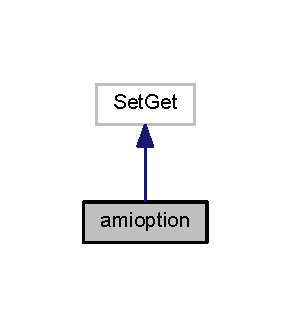
\includegraphics[width=139pt]{classamioption__inherit__graph}
\end{center}
\end{figure}


Collaboration diagram for amioption\+:\nopagebreak
\begin{figure}[H]
\begin{center}
\leavevmode
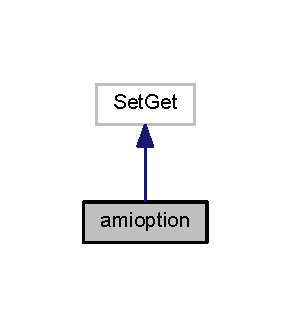
\includegraphics[width=139pt]{classamioption__coll__graph}
\end{center}
\end{figure}
\subsubsection*{Public Member Functions}
\begin{DoxyCompactItemize}
\item 
\hyperlink{classamioption_a86c655c4010c1c2ddb3e68693a07ef37}{amioption} (matlabtypesubstitute varargin)
\begin{DoxyCompactList}\small\item\em amioptions Construct a new amioptions object \end{DoxyCompactList}\end{DoxyCompactItemize}
\subsubsection*{Public Attributes}
\begin{DoxyCompactItemize}
\item 
matlabtypesubstitute \hyperlink{classamioption_a0c5f3dcf809a17b895fe12fc91272349}{atol} = 1e-\/16
\begin{DoxyCompactList}\small\item\em absolute integration tolerace \end{DoxyCompactList}\item 
matlabtypesubstitute \hyperlink{classamioption_a7978e9a4674f869e6b2950e2f6262ca5}{rtol} = 1e-\/8
\begin{DoxyCompactList}\small\item\em relative integration tolerace \end{DoxyCompactList}\item 
matlabtypesubstitute \hyperlink{classamioption_ac37622882dacee1f11688d4941ccb45e}{maxsteps} = 1e4
\begin{DoxyCompactList}\small\item\em maximum number of integration steps \end{DoxyCompactList}\item 
matlabtypesubstitute \hyperlink{classamioption_a0505783cf66f362672cbe3320d47a94d}{sens\+\_\+ind} = double.\+empty(\char`\"{}\char`\"{})
\begin{DoxyCompactList}\small\item\em index of parameters for which the sensitivities are computed \end{DoxyCompactList}\item 
matlabtypesubstitute \hyperlink{classamioption_a8938c19fd7067f4780be8255764210b7}{qpositivex} = double.\+empty(\char`\"{}\char`\"{})
\begin{DoxyCompactList}\small\item\em index of states for which positivity should be enforced (currently this has no effect) \end{DoxyCompactList}\item 
matlabtypesubstitute \hyperlink{classamioption_a18a69d8713604897ca9ee705d9d4fc4a}{tstart} = 0
\begin{DoxyCompactList}\small\item\em starting time of the simulation \end{DoxyCompactList}\item 
matlabtypesubstitute \hyperlink{classamioption_a6f4b21b13e0c8c531c452c70b43fc96a}{lmm} = 2
\begin{DoxyCompactList}\small\item\em linear multistep method. \end{DoxyCompactList}\item 
matlabtypesubstitute \hyperlink{classamioption_a1fc3ae6bd5c6a80e9b81b27fc7b7a11a}{iter} = 2
\begin{DoxyCompactList}\small\item\em iteration method for linear multistep. \end{DoxyCompactList}\item 
matlabtypesubstitute \hyperlink{classamioption_a06749b49eaa313f4d00f0115d3a7a7f3}{linsol} = 9
\begin{DoxyCompactList}\small\item\em linear solver \end{DoxyCompactList}\item 
matlabtypesubstitute \hyperlink{classamioption_a202e02f7d8c1a87b1c675bcc1acf1c8e}{stldet} = true
\begin{DoxyCompactList}\small\item\em stability detection flag \end{DoxyCompactList}\item 
matlabtypesubstitute \hyperlink{classamioption_ad06cc805fa18b06ac937fd98a9eba0e7}{interp\+Type} = 1
\begin{DoxyCompactList}\small\item\em interpolation type \end{DoxyCompactList}\item 
matlabtypesubstitute \hyperlink{classamioption_afbc60e75d11740bf27f5a7fc5706fd44}{lmm\+B} = 2
\begin{DoxyCompactList}\small\item\em linear multistep method (backwards) \end{DoxyCompactList}\item 
matlabtypesubstitute \hyperlink{classamioption_ae6a49cec21ffe790217be29b0fced832}{iter\+B} = 2
\begin{DoxyCompactList}\small\item\em iteration method for linear multistep (backwards). \end{DoxyCompactList}\item 
matlabtypesubstitute \hyperlink{classamioption_aada9d6834569ad5c542cb8dc6b26ea46}{ism} = 1
\begin{DoxyCompactList}\small\item\em forward sensitivity mode \end{DoxyCompactList}\item 
matlabtypesubstitute \hyperlink{classamioption_ab31e219eb42bc06629c3f247a01b9906}{sensi\+\_\+meth} = 1
\begin{DoxyCompactList}\small\item\em sensitivity method \end{DoxyCompactList}\item 
matlabtypesubstitute \hyperlink{classamioption_a7dd31d33463c5a709251bcef0eccaa36}{sensi} = 0
\begin{DoxyCompactList}\small\item\em sensitivity order \end{DoxyCompactList}\item 
matlabtypesubstitute \hyperlink{classamioption_a85519d27e7231ac625e5b2deee92165a}{nmaxevent} = 10
\begin{DoxyCompactList}\small\item\em number of reported events \end{DoxyCompactList}\item 
matlabtypesubstitute \hyperlink{classamioption_aa5d555210685086c19e5d08afca6685b}{ordering} = 1
\begin{DoxyCompactList}\small\item\em reordering of states \end{DoxyCompactList}\item 
matlabtypesubstitute \hyperlink{classamioption_a8f60c8102d29fcd525162d02eed4566b}{ss} = 0
\begin{DoxyCompactList}\small\item\em steady state sensitivity flag \end{DoxyCompactList}\item 
matlabtypesubstitute \hyperlink{classamioption_ae40f9a7172d3a41725c151afaec347f7}{sx0} = double.\+empty(\char`\"{}\char`\"{})
\begin{DoxyCompactList}\small\item\em custom initial sensitivity \end{DoxyCompactList}\item 
matlabtypesubstitute \hyperlink{classamioption_a7a7be015feeb7a346dceccd49e622b4b}{z2event} = double.\+empty(\char`\"{}\char`\"{})
\begin{DoxyCompactList}\small\item\em mapping of event ouputs to events \end{DoxyCompactList}\item 
matlabtypesubstitute \hyperlink{classamioption_acf2488b95c97e0378c9bf49de3b50f28}{id} = double.\+empty(\char`\"{}\char`\"{})
\begin{DoxyCompactList}\small\item\em flag for D\+A\+E variables \end{DoxyCompactList}\end{DoxyCompactItemize}


\subsubsection{Detailed Description}


Definition at line 17 of file amioption.\+m.



\subsubsection{Constructor \& Destructor Documentation}
\hypertarget{classamioption_a86c655c4010c1c2ddb3e68693a07ef37}{}\index{amioption@{amioption}!amioption@{amioption}}
\index{amioption@{amioption}!amioption@{amioption}}
\paragraph[{amioption(matlabtypesubstitute varargin)}]{\setlength{\rightskip}{0pt plus 5cm}{\bf amioption} (
\begin{DoxyParamCaption}
\item[{matlabtypesubstitute}]{varargin}
\end{DoxyParamCaption}
)}\label{classamioption_a86c655c4010c1c2ddb3e68693a07ef37}
O\+P\+T\+S = \hyperlink{classamioption_a86c655c4010c1c2ddb3e68693a07ef37}{amioption()} creates a set of options with each option set to its default value.

O\+P\+T\+S = amioption(P\+A\+R\+A\+M, V\+A\+L, ...) creates a set of options with the named parameters altered with the specified values.

O\+P\+T\+S = amioption(O\+L\+D\+O\+P\+T\+S, P\+A\+R\+A\+M, V\+A\+L, ...) creates a copy of O\+L\+D\+O\+P\+T\+S with the named parameters altered with the specified value

Note to see the parameters, check the documentation page for amioptions 

Definition at line 217 of file amioption.\+m.



\subsubsection{Member Data Documentation}
\hypertarget{classamioption_a0c5f3dcf809a17b895fe12fc91272349}{}\index{amioption@{amioption}!atol@{atol}}
\index{atol@{atol}!amioption@{amioption}}
\paragraph[{atol}]{\setlength{\rightskip}{0pt plus 5cm}atol = 1e-\/16}\label{classamioption_a0c5f3dcf809a17b895fe12fc91272349}
~\newline
{\bfseries Default\+:} 1e-\/16 

Definition at line 28 of file amioption.\+m.

\hypertarget{classamioption_a7978e9a4674f869e6b2950e2f6262ca5}{}\index{amioption@{amioption}!rtol@{rtol}}
\index{rtol@{rtol}!amioption@{amioption}}
\paragraph[{rtol}]{\setlength{\rightskip}{0pt plus 5cm}rtol = 1e-\/8}\label{classamioption_a7978e9a4674f869e6b2950e2f6262ca5}
~\newline
{\bfseries Default\+:} 1e-\/8 

Definition at line 36 of file amioption.\+m.

\hypertarget{classamioption_ac37622882dacee1f11688d4941ccb45e}{}\index{amioption@{amioption}!maxsteps@{maxsteps}}
\index{maxsteps@{maxsteps}!amioption@{amioption}}
\paragraph[{maxsteps}]{\setlength{\rightskip}{0pt plus 5cm}maxsteps = 1e4}\label{classamioption_ac37622882dacee1f11688d4941ccb45e}
~\newline
{\bfseries Default\+:} 1e4 

Definition at line 44 of file amioption.\+m.

\hypertarget{classamioption_a0505783cf66f362672cbe3320d47a94d}{}\index{amioption@{amioption}!sens\+\_\+ind@{sens\+\_\+ind}}
\index{sens\+\_\+ind@{sens\+\_\+ind}!amioption@{amioption}}
\paragraph[{sens\+\_\+ind}]{\setlength{\rightskip}{0pt plus 5cm}sens\+\_\+ind = double.\+empty(\char`\"{}\char`\"{})}\label{classamioption_a0505783cf66f362672cbe3320d47a94d}
~\newline
{\bfseries Default\+:} double.\+empty(\char`\"{}\char`\"{}) 

Definition at line 52 of file amioption.\+m.

\hypertarget{classamioption_a8938c19fd7067f4780be8255764210b7}{}\index{amioption@{amioption}!qpositivex@{qpositivex}}
\index{qpositivex@{qpositivex}!amioption@{amioption}}
\paragraph[{qpositivex}]{\setlength{\rightskip}{0pt plus 5cm}qpositivex = double.\+empty(\char`\"{}\char`\"{})}\label{classamioption_a8938c19fd7067f4780be8255764210b7}
~\newline
{\bfseries Default\+:} double.\+empty(\char`\"{}\char`\"{}) 

Definition at line 60 of file amioption.\+m.

\hypertarget{classamioption_a18a69d8713604897ca9ee705d9d4fc4a}{}\index{amioption@{amioption}!tstart@{tstart}}
\index{tstart@{tstart}!amioption@{amioption}}
\paragraph[{tstart}]{\setlength{\rightskip}{0pt plus 5cm}tstart = 0}\label{classamioption_a18a69d8713604897ca9ee705d9d4fc4a}
~\newline
{\bfseries Default\+:} 0 

Definition at line 69 of file amioption.\+m.

\hypertarget{classamioption_a6f4b21b13e0c8c531c452c70b43fc96a}{}\index{amioption@{amioption}!lmm@{lmm}}
\index{lmm@{lmm}!amioption@{amioption}}
\paragraph[{lmm}]{\setlength{\rightskip}{0pt plus 5cm}lmm = 2}\label{classamioption_a6f4b21b13e0c8c531c452c70b43fc96a}
~\newline
{\bfseries Default\+:} 2 

Definition at line 77 of file amioption.\+m.

\hypertarget{classamioption_a1fc3ae6bd5c6a80e9b81b27fc7b7a11a}{}\index{amioption@{amioption}!iter@{iter}}
\index{iter@{iter}!amioption@{amioption}}
\paragraph[{iter}]{\setlength{\rightskip}{0pt plus 5cm}iter = 2}\label{classamioption_a1fc3ae6bd5c6a80e9b81b27fc7b7a11a}
~\newline
{\bfseries Default\+:} 2 

Definition at line 85 of file amioption.\+m.

\hypertarget{classamioption_a06749b49eaa313f4d00f0115d3a7a7f3}{}\index{amioption@{amioption}!linsol@{linsol}}
\index{linsol@{linsol}!amioption@{amioption}}
\paragraph[{linsol}]{\setlength{\rightskip}{0pt plus 5cm}linsol = 9}\label{classamioption_a06749b49eaa313f4d00f0115d3a7a7f3}
~\newline
{\bfseries Default\+:} 9 

Definition at line 93 of file amioption.\+m.

\hypertarget{classamioption_a202e02f7d8c1a87b1c675bcc1acf1c8e}{}\index{amioption@{amioption}!stldet@{stldet}}
\index{stldet@{stldet}!amioption@{amioption}}
\paragraph[{stldet}]{\setlength{\rightskip}{0pt plus 5cm}stldet = true}\label{classamioption_a202e02f7d8c1a87b1c675bcc1acf1c8e}
~\newline
{\bfseries Default\+:} true 

Definition at line 101 of file amioption.\+m.

\hypertarget{classamioption_ad06cc805fa18b06ac937fd98a9eba0e7}{}\index{amioption@{amioption}!interp\+Type@{interp\+Type}}
\index{interp\+Type@{interp\+Type}!amioption@{amioption}}
\paragraph[{interp\+Type}]{\setlength{\rightskip}{0pt plus 5cm}interp\+Type = 1}\label{classamioption_ad06cc805fa18b06ac937fd98a9eba0e7}
~\newline
{\bfseries Default\+:} 1 

Definition at line 109 of file amioption.\+m.

\hypertarget{classamioption_afbc60e75d11740bf27f5a7fc5706fd44}{}\index{amioption@{amioption}!lmm\+B@{lmm\+B}}
\index{lmm\+B@{lmm\+B}!amioption@{amioption}}
\paragraph[{lmm\+B}]{\setlength{\rightskip}{0pt plus 5cm}lmm\+B = 2}\label{classamioption_afbc60e75d11740bf27f5a7fc5706fd44}
~\newline
{\bfseries Default\+:} 2 

Definition at line 117 of file amioption.\+m.

\hypertarget{classamioption_ae6a49cec21ffe790217be29b0fced832}{}\index{amioption@{amioption}!iter\+B@{iter\+B}}
\index{iter\+B@{iter\+B}!amioption@{amioption}}
\paragraph[{iter\+B}]{\setlength{\rightskip}{0pt plus 5cm}iter\+B = 2}\label{classamioption_ae6a49cec21ffe790217be29b0fced832}
~\newline
{\bfseries Default\+:} 2 

Definition at line 125 of file amioption.\+m.

\hypertarget{classamioption_aada9d6834569ad5c542cb8dc6b26ea46}{}\index{amioption@{amioption}!ism@{ism}}
\index{ism@{ism}!amioption@{amioption}}
\paragraph[{ism}]{\setlength{\rightskip}{0pt plus 5cm}ism = 1}\label{classamioption_aada9d6834569ad5c542cb8dc6b26ea46}
~\newline
{\bfseries Default\+:} 1 

Definition at line 133 of file amioption.\+m.

\hypertarget{classamioption_ab31e219eb42bc06629c3f247a01b9906}{}\index{amioption@{amioption}!sensi\+\_\+meth@{sensi\+\_\+meth}}
\index{sensi\+\_\+meth@{sensi\+\_\+meth}!amioption@{amioption}}
\paragraph[{sensi\+\_\+meth}]{\setlength{\rightskip}{0pt plus 5cm}sensi\+\_\+meth = 1}\label{classamioption_ab31e219eb42bc06629c3f247a01b9906}
~\newline
{\bfseries Default\+:} 1

\begin{DoxyNote}{Note}
This property has custom functionality when its value is changed. 
\end{DoxyNote}


Definition at line 141 of file amioption.\+m.

\hypertarget{classamioption_a7dd31d33463c5a709251bcef0eccaa36}{}\index{amioption@{amioption}!sensi@{sensi}}
\index{sensi@{sensi}!amioption@{amioption}}
\paragraph[{sensi}]{\setlength{\rightskip}{0pt plus 5cm}sensi = 0}\label{classamioption_a7dd31d33463c5a709251bcef0eccaa36}
~\newline
{\bfseries Default\+:} 0

\begin{DoxyNote}{Note}
This property has custom functionality when its value is changed. 
\end{DoxyNote}


Definition at line 149 of file amioption.\+m.

\hypertarget{classamioption_a85519d27e7231ac625e5b2deee92165a}{}\index{amioption@{amioption}!nmaxevent@{nmaxevent}}
\index{nmaxevent@{nmaxevent}!amioption@{amioption}}
\paragraph[{nmaxevent}]{\setlength{\rightskip}{0pt plus 5cm}nmaxevent = 10}\label{classamioption_a85519d27e7231ac625e5b2deee92165a}
~\newline
{\bfseries Default\+:} 10 

Definition at line 157 of file amioption.\+m.

\hypertarget{classamioption_aa5d555210685086c19e5d08afca6685b}{}\index{amioption@{amioption}!ordering@{ordering}}
\index{ordering@{ordering}!amioption@{amioption}}
\paragraph[{ordering}]{\setlength{\rightskip}{0pt plus 5cm}ordering = 1}\label{classamioption_aa5d555210685086c19e5d08afca6685b}
~\newline
{\bfseries Default\+:} 1 

Definition at line 165 of file amioption.\+m.

\hypertarget{classamioption_a8f60c8102d29fcd525162d02eed4566b}{}\index{amioption@{amioption}!ss@{ss}}
\index{ss@{ss}!amioption@{amioption}}
\paragraph[{ss}]{\setlength{\rightskip}{0pt plus 5cm}ss = 0}\label{classamioption_a8f60c8102d29fcd525162d02eed4566b}
~\newline
{\bfseries Default\+:} 0 

Definition at line 173 of file amioption.\+m.

\hypertarget{classamioption_ae40f9a7172d3a41725c151afaec347f7}{}\index{amioption@{amioption}!sx0@{sx0}}
\index{sx0@{sx0}!amioption@{amioption}}
\paragraph[{sx0}]{\setlength{\rightskip}{0pt plus 5cm}sx0 = double.\+empty(\char`\"{}\char`\"{})}\label{classamioption_ae40f9a7172d3a41725c151afaec347f7}
~\newline
{\bfseries Default\+:} double.\+empty(\char`\"{}\char`\"{}) 

Definition at line 181 of file amioption.\+m.

\hypertarget{classamioption_a7a7be015feeb7a346dceccd49e622b4b}{}\index{amioption@{amioption}!z2event@{z2event}}
\index{z2event@{z2event}!amioption@{amioption}}
\paragraph[{z2event}]{\setlength{\rightskip}{0pt plus 5cm}z2event = double.\+empty(\char`\"{}\char`\"{})}\label{classamioption_a7a7be015feeb7a346dceccd49e622b4b}
\begin{DoxyNote}{Note}
This property has the M\+A\+T\+L\+A\+B attribute {\ttfamily Hidden} set to true. 

\href{http://www.mathworks.com/help/matlab/matlab_oop/property-attributes.html}{\tt Matlab documentation of property attributes.} ~\newline
{\bfseries Default\+:} double.\+empty(\char`\"{}\char`\"{}) 
\end{DoxyNote}


Definition at line 192 of file amioption.\+m.

\hypertarget{classamioption_acf2488b95c97e0378c9bf49de3b50f28}{}\index{amioption@{amioption}!id@{id}}
\index{id@{id}!amioption@{amioption}}
\paragraph[{id}]{\setlength{\rightskip}{0pt plus 5cm}id = double.\+empty(\char`\"{}\char`\"{})}\label{classamioption_acf2488b95c97e0378c9bf49de3b50f28}
\begin{DoxyNote}{Note}
This property has the M\+A\+T\+L\+A\+B attribute {\ttfamily Hidden} set to true. 

\href{http://www.mathworks.com/help/matlab/matlab_oop/property-attributes.html}{\tt Matlab documentation of property attributes.} ~\newline
{\bfseries Default\+:} double.\+empty(\char`\"{}\char`\"{}) 
\end{DoxyNote}


Definition at line 203 of file amioption.\+m.


\hypertarget{struct_exp_data}{}\subsection{Exp\+Data Struct Reference}
\label{struct_exp_data}\index{Exp\+Data@{Exp\+Data}}


struct that carries all information about experimental data  




{\ttfamily \#include $<$edata.\+h$>$}

\subsubsection*{Public Attributes}
\begin{DoxyCompactItemize}
\item 
double $\ast$ \hyperlink{struct_exp_data_a1853cfbbd72291b3c37df42b7f07d513}{am\+\_\+my}
\item 
double $\ast$ \hyperlink{struct_exp_data_af29a27d415ab3b3f165e86473412baad}{am\+\_\+ysigma}
\item 
double $\ast$ \hyperlink{struct_exp_data_a847258093bc307817a8c9cedc3f5edc3}{am\+\_\+mz}
\item 
double $\ast$ \hyperlink{struct_exp_data_a806c9883d66f002acdcceaeda3e57fb2}{am\+\_\+zsigma}
\end{DoxyCompactItemize}


\subsubsection{Detailed Description}


Definition at line 18 of file edata.\+h.



\subsubsection{Member Data Documentation}
\hypertarget{struct_exp_data_a1853cfbbd72291b3c37df42b7f07d513}{}\index{Exp\+Data@{Exp\+Data}!am\+\_\+my@{am\+\_\+my}}
\index{am\+\_\+my@{am\+\_\+my}!Exp\+Data@{Exp\+Data}}
\paragraph[{am\+\_\+my}]{\setlength{\rightskip}{0pt plus 5cm}double$\ast$ am\+\_\+my}\label{struct_exp_data_a1853cfbbd72291b3c37df42b7f07d513}
observed data 

Definition at line 20 of file edata.\+h.

\hypertarget{struct_exp_data_af29a27d415ab3b3f165e86473412baad}{}\index{Exp\+Data@{Exp\+Data}!am\+\_\+ysigma@{am\+\_\+ysigma}}
\index{am\+\_\+ysigma@{am\+\_\+ysigma}!Exp\+Data@{Exp\+Data}}
\paragraph[{am\+\_\+ysigma}]{\setlength{\rightskip}{0pt plus 5cm}double$\ast$ am\+\_\+ysigma}\label{struct_exp_data_af29a27d415ab3b3f165e86473412baad}
standard deviation of observed data 

Definition at line 22 of file edata.\+h.

\hypertarget{struct_exp_data_a847258093bc307817a8c9cedc3f5edc3}{}\index{Exp\+Data@{Exp\+Data}!am\+\_\+mz@{am\+\_\+mz}}
\index{am\+\_\+mz@{am\+\_\+mz}!Exp\+Data@{Exp\+Data}}
\paragraph[{am\+\_\+mz}]{\setlength{\rightskip}{0pt plus 5cm}double$\ast$ am\+\_\+mz}\label{struct_exp_data_a847258093bc307817a8c9cedc3f5edc3}
observed events 

Definition at line 25 of file edata.\+h.

\hypertarget{struct_exp_data_a806c9883d66f002acdcceaeda3e57fb2}{}\index{Exp\+Data@{Exp\+Data}!am\+\_\+zsigma@{am\+\_\+zsigma}}
\index{am\+\_\+zsigma@{am\+\_\+zsigma}!Exp\+Data@{Exp\+Data}}
\paragraph[{am\+\_\+zsigma}]{\setlength{\rightskip}{0pt plus 5cm}double$\ast$ am\+\_\+zsigma}\label{struct_exp_data_a806c9883d66f002acdcceaeda3e57fb2}
standard deviation of observed events 

Definition at line 27 of file edata.\+h.


\hypertarget{classfun_test}{}\subsection{fun\+Test Class Reference}
\label{classfun_test}\index{fun\+Test@{fun\+Test}}


F\+U\+N\+T\+E\+S\+T Summary of this class goes here Detailed explanation goes here.  




\subsubsection{Detailed Description}


Definition at line 17 of file fun\+Test.\+m.


\hypertarget{classmodel_test}{}\subsection{model\+Test Class Reference}
\label{classmodel_test}\index{model\+Test@{model\+Test}}


M\+O\+D\+E\+L\+T\+E\+S\+T Summary of this class goes here Detailed explanation goes here.  




\subsubsection{Detailed Description}


Definition at line 17 of file model\+Test.\+m.


\hypertarget{classoptsym}{}\doxysubsection{optsym Class Reference}
\label{classoptsym}\index{optsym@{optsym}}


O\+P\+T\+S\+YM is an auxiliary class to gain access to the private symbolic property {\ttfamily s} which is necessary to be able to call symobj\+::optimize on it.  




Inheritance diagram for optsym\+:
\nopagebreak
\begin{figure}[H]
\begin{center}
\leavevmode
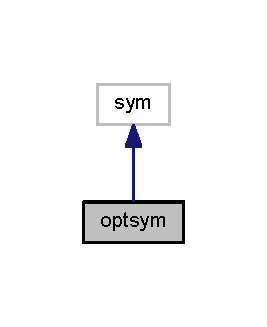
\includegraphics[width=129pt]{classoptsym__inherit__graph}
\end{center}
\end{figure}
\doxysubsubsection*{Public Member Functions}
\begin{DoxyCompactItemize}
\item 
\mbox{\hyperlink{classoptsym_afe9ab2368d1b1705d6a38ae4ed7dcb37}{optsym}} (\+::sym symbol)
\begin{DoxyCompactList}\small\item\em optsym converts the symbolic object into a optsym object \end{DoxyCompactList}\item 
mlhs\+Inner\+Subst$<$\+::sym $>$ \mbox{\hyperlink{classoptsym_a9025fce18af7d11fcca43332aece29bc}{getoptimized}} ()
\begin{DoxyCompactList}\small\item\em getoptimized calls symobj\+::optimize on the optsym object \end{DoxyCompactList}\end{DoxyCompactItemize}


\doxysubsubsection{Detailed Description}


Definition at line 17 of file optsym.\+m.



\doxysubsubsection{Constructor \& Destructor Documentation}
\mbox{\Hypertarget{classoptsym_afe9ab2368d1b1705d6a38ae4ed7dcb37}\label{classoptsym_afe9ab2368d1b1705d6a38ae4ed7dcb37}} 
\index{optsym@{optsym}!optsym@{optsym}}
\index{optsym@{optsym}!optsym@{optsym}}
\doxyparagraph{\texorpdfstring{optsym()}{optsym()}}
{\footnotesize\ttfamily \mbox{\hyperlink{classoptsym}{optsym}} (\begin{DoxyParamCaption}\item[{\+::sym}]{symbol }\end{DoxyParamCaption})}


\begin{DoxyParams}{Parameters}
{\em symbol} & symbolic object \\
\hline
\end{DoxyParams}


Definition at line 32 of file optsym.\+m.



\doxysubsubsection{Member Function Documentation}
\mbox{\Hypertarget{classoptsym_a9025fce18af7d11fcca43332aece29bc}\label{classoptsym_a9025fce18af7d11fcca43332aece29bc}} 
\index{optsym@{optsym}!getoptimized@{getoptimized}}
\index{getoptimized@{getoptimized}!optsym@{optsym}}
\doxyparagraph{\texorpdfstring{getoptimized()}{getoptimized()}}
{\footnotesize\ttfamily mlhs\+Inner\+Subst$<$\+::sym $>$ getoptimized (\begin{DoxyParamCaption}{ }\end{DoxyParamCaption})}


\begin{DoxyRetVals}{Return values}
{\em out} & optimized symbolic object \\
\hline
\end{DoxyRetVals}


Definition at line 42 of file optsym.\+m.


\hypertarget{struct_return_data}{}\subsection{Return\+Data Struct Reference}
\label{struct_return_data}\index{Return\+Data@{Return\+Data}}


struct that stores all data which is later returned by the mex function  




{\ttfamily \#include $<$rdata.\+h$>$}

\subsubsection*{Public Attributes}
\begin{DoxyCompactItemize}
\item 
double $\ast$ \hyperlink{struct_return_data_a577298549da7c9dbe3d93fbf3bc17866}{am\+\_\+tsdata}
\item 
double $\ast$ \hyperlink{struct_return_data_a3ea8fa08fcced0827c1df276b0d253c8}{am\+\_\+xdotdata}
\item 
double $\ast$ \hyperlink{struct_return_data_a494b13e9797d95d7fb3c89e09864aa4f}{am\+\_\+dxdotdpdata}
\item 
double $\ast$ \hyperlink{struct_return_data_a831cada35b4f407a2c8ad789dfc534e5}{am\+\_\+dydxdata}
\item 
double $\ast$ \hyperlink{struct_return_data_a57a7eb2085d8ed5bb6c62331a2aa3af5}{am\+\_\+dydpdata}
\item 
double $\ast$ \hyperlink{struct_return_data_a82d71415ca06c969ebd22a02e4789b1d}{am\+\_\+\+Jdata}
\item 
double $\ast$ \hyperlink{struct_return_data_af1a09a94b46b2a4e6b3e90d37a7fdbe3}{am\+\_\+rootdata}
\item 
double $\ast$ \hyperlink{struct_return_data_a98be71879a3ad48c62a203c0a03457f5}{am\+\_\+root\+Sdata}
\item 
double $\ast$ \hyperlink{struct_return_data_a4d7116a416a12564e8058589889357ba}{am\+\_\+root\+S2data}
\item 
double $\ast$ \hyperlink{struct_return_data_a4991fdb926d3db2f28c327165d0c11c4}{am\+\_\+rootvaldata}
\item 
double $\ast$ \hyperlink{struct_return_data_adc0a319cb427b2ad2fef3f2cbd69d765}{am\+\_\+rootval\+Sdata}
\item 
double $\ast$ \hyperlink{struct_return_data_a63a3d2f728c5789c4b93a84ecaf29cfa}{am\+\_\+rootval\+S2data}
\item 
double $\ast$ \hyperlink{struct_return_data_ad99b08eb835733c2416a1a0004e4a491}{am\+\_\+xdata}
\item 
double $\ast$ \hyperlink{struct_return_data_a097369567440c923ac24256e75ab3e89}{am\+\_\+x\+Sdata}
\item 
double $\ast$ \hyperlink{struct_return_data_a24568582aa8de699ea1ce53323ff26ca}{am\+\_\+ydata}
\item 
double $\ast$ \hyperlink{struct_return_data_aa2089cdd16d3cb3c9b85f99f570197d1}{am\+\_\+y\+Sdata}
\item 
double $\ast$ \hyperlink{struct_return_data_a2ebada170b4bc6a2337794e4ec08d77c}{am\+\_\+numstepsdata}
\item 
double $\ast$ \hyperlink{struct_return_data_a6852d3762d59842903ef737ed511dc43}{am\+\_\+numsteps\+Sdata}
\item 
double $\ast$ \hyperlink{struct_return_data_a480d4eb0a1a568f64b8e939105a0b627}{am\+\_\+numrhsevalsdata}
\item 
double $\ast$ \hyperlink{struct_return_data_a77e958126968de6f5ee3bd1d22129641}{am\+\_\+numrhsevals\+Sdata}
\item 
double $\ast$ \hyperlink{struct_return_data_af792e4a1c5c23c5232ef9398e25de1a7}{am\+\_\+orderdata}
\item 
double $\ast$ \hyperlink{struct_return_data_af95fa143e0e524652f9a818f6288b544}{am\+\_\+llhdata}
\item 
double $\ast$ \hyperlink{struct_return_data_ae0fc05ce8c52bdda5c7bff541c79945d}{am\+\_\+chi2data}
\item 
double $\ast$ \hyperlink{struct_return_data_af72a5801bf4c6b957812c8b2471ecf41}{am\+\_\+llh\+Sdata}
\item 
double $\ast$ \hyperlink{struct_return_data_a9ea6527fa5408fa1ae074cdbd83ed11f}{am\+\_\+llh\+S2data}
\end{DoxyCompactItemize}


\subsubsection{Detailed Description}


Definition at line 42 of file rdata.\+h.



\subsubsection{Member Data Documentation}
\hypertarget{struct_return_data_a577298549da7c9dbe3d93fbf3bc17866}{}\index{Return\+Data@{Return\+Data}!am\+\_\+tsdata@{am\+\_\+tsdata}}
\index{am\+\_\+tsdata@{am\+\_\+tsdata}!Return\+Data@{Return\+Data}}
\paragraph[{am\+\_\+tsdata}]{\setlength{\rightskip}{0pt plus 5cm}double$\ast$ am\+\_\+tsdata}\label{struct_return_data_a577298549da7c9dbe3d93fbf3bc17866}
timepoints 

Definition at line 45 of file rdata.\+h.

\hypertarget{struct_return_data_a3ea8fa08fcced0827c1df276b0d253c8}{}\index{Return\+Data@{Return\+Data}!am\+\_\+xdotdata@{am\+\_\+xdotdata}}
\index{am\+\_\+xdotdata@{am\+\_\+xdotdata}!Return\+Data@{Return\+Data}}
\paragraph[{am\+\_\+xdotdata}]{\setlength{\rightskip}{0pt plus 5cm}double$\ast$ am\+\_\+xdotdata}\label{struct_return_data_a3ea8fa08fcced0827c1df276b0d253c8}
time derivative 

Definition at line 47 of file rdata.\+h.

\hypertarget{struct_return_data_a494b13e9797d95d7fb3c89e09864aa4f}{}\index{Return\+Data@{Return\+Data}!am\+\_\+dxdotdpdata@{am\+\_\+dxdotdpdata}}
\index{am\+\_\+dxdotdpdata@{am\+\_\+dxdotdpdata}!Return\+Data@{Return\+Data}}
\paragraph[{am\+\_\+dxdotdpdata}]{\setlength{\rightskip}{0pt plus 5cm}double$\ast$ am\+\_\+dxdotdpdata}\label{struct_return_data_a494b13e9797d95d7fb3c89e09864aa4f}
parameter derivative of time derivative 

Definition at line 49 of file rdata.\+h.

\hypertarget{struct_return_data_a831cada35b4f407a2c8ad789dfc534e5}{}\index{Return\+Data@{Return\+Data}!am\+\_\+dydxdata@{am\+\_\+dydxdata}}
\index{am\+\_\+dydxdata@{am\+\_\+dydxdata}!Return\+Data@{Return\+Data}}
\paragraph[{am\+\_\+dydxdata}]{\setlength{\rightskip}{0pt plus 5cm}double$\ast$ am\+\_\+dydxdata}\label{struct_return_data_a831cada35b4f407a2c8ad789dfc534e5}
state derivative of observables 

Definition at line 51 of file rdata.\+h.

\hypertarget{struct_return_data_a57a7eb2085d8ed5bb6c62331a2aa3af5}{}\index{Return\+Data@{Return\+Data}!am\+\_\+dydpdata@{am\+\_\+dydpdata}}
\index{am\+\_\+dydpdata@{am\+\_\+dydpdata}!Return\+Data@{Return\+Data}}
\paragraph[{am\+\_\+dydpdata}]{\setlength{\rightskip}{0pt plus 5cm}double$\ast$ am\+\_\+dydpdata}\label{struct_return_data_a57a7eb2085d8ed5bb6c62331a2aa3af5}
parameter derivative of observables 

Definition at line 53 of file rdata.\+h.

\hypertarget{struct_return_data_a82d71415ca06c969ebd22a02e4789b1d}{}\index{Return\+Data@{Return\+Data}!am\+\_\+\+Jdata@{am\+\_\+\+Jdata}}
\index{am\+\_\+\+Jdata@{am\+\_\+\+Jdata}!Return\+Data@{Return\+Data}}
\paragraph[{am\+\_\+\+Jdata}]{\setlength{\rightskip}{0pt plus 5cm}double$\ast$ am\+\_\+\+Jdata}\label{struct_return_data_a82d71415ca06c969ebd22a02e4789b1d}
Jacobian of differential equation right hand side 

Definition at line 55 of file rdata.\+h.

\hypertarget{struct_return_data_af1a09a94b46b2a4e6b3e90d37a7fdbe3}{}\index{Return\+Data@{Return\+Data}!am\+\_\+rootdata@{am\+\_\+rootdata}}
\index{am\+\_\+rootdata@{am\+\_\+rootdata}!Return\+Data@{Return\+Data}}
\paragraph[{am\+\_\+rootdata}]{\setlength{\rightskip}{0pt plus 5cm}double$\ast$ am\+\_\+rootdata}\label{struct_return_data_af1a09a94b46b2a4e6b3e90d37a7fdbe3}
events 

Definition at line 57 of file rdata.\+h.

\hypertarget{struct_return_data_a98be71879a3ad48c62a203c0a03457f5}{}\index{Return\+Data@{Return\+Data}!am\+\_\+root\+Sdata@{am\+\_\+root\+Sdata}}
\index{am\+\_\+root\+Sdata@{am\+\_\+root\+Sdata}!Return\+Data@{Return\+Data}}
\paragraph[{am\+\_\+root\+Sdata}]{\setlength{\rightskip}{0pt plus 5cm}double$\ast$ am\+\_\+root\+Sdata}\label{struct_return_data_a98be71879a3ad48c62a203c0a03457f5}
parameter derivative of events 

Definition at line 59 of file rdata.\+h.

\hypertarget{struct_return_data_a4d7116a416a12564e8058589889357ba}{}\index{Return\+Data@{Return\+Data}!am\+\_\+root\+S2data@{am\+\_\+root\+S2data}}
\index{am\+\_\+root\+S2data@{am\+\_\+root\+S2data}!Return\+Data@{Return\+Data}}
\paragraph[{am\+\_\+root\+S2data}]{\setlength{\rightskip}{0pt plus 5cm}double$\ast$ am\+\_\+root\+S2data}\label{struct_return_data_a4d7116a416a12564e8058589889357ba}
second order parameter derivative of events 

Definition at line 61 of file rdata.\+h.

\hypertarget{struct_return_data_a4991fdb926d3db2f28c327165d0c11c4}{}\index{Return\+Data@{Return\+Data}!am\+\_\+rootvaldata@{am\+\_\+rootvaldata}}
\index{am\+\_\+rootvaldata@{am\+\_\+rootvaldata}!Return\+Data@{Return\+Data}}
\paragraph[{am\+\_\+rootvaldata}]{\setlength{\rightskip}{0pt plus 5cm}double$\ast$ am\+\_\+rootvaldata}\label{struct_return_data_a4991fdb926d3db2f28c327165d0c11c4}
value of event function 

Definition at line 63 of file rdata.\+h.

\hypertarget{struct_return_data_adc0a319cb427b2ad2fef3f2cbd69d765}{}\index{Return\+Data@{Return\+Data}!am\+\_\+rootval\+Sdata@{am\+\_\+rootval\+Sdata}}
\index{am\+\_\+rootval\+Sdata@{am\+\_\+rootval\+Sdata}!Return\+Data@{Return\+Data}}
\paragraph[{am\+\_\+rootval\+Sdata}]{\setlength{\rightskip}{0pt plus 5cm}double$\ast$ am\+\_\+rootval\+Sdata}\label{struct_return_data_adc0a319cb427b2ad2fef3f2cbd69d765}
parameter derivative of event function 

Definition at line 65 of file rdata.\+h.

\hypertarget{struct_return_data_a63a3d2f728c5789c4b93a84ecaf29cfa}{}\index{Return\+Data@{Return\+Data}!am\+\_\+rootval\+S2data@{am\+\_\+rootval\+S2data}}
\index{am\+\_\+rootval\+S2data@{am\+\_\+rootval\+S2data}!Return\+Data@{Return\+Data}}
\paragraph[{am\+\_\+rootval\+S2data}]{\setlength{\rightskip}{0pt plus 5cm}double$\ast$ am\+\_\+rootval\+S2data}\label{struct_return_data_a63a3d2f728c5789c4b93a84ecaf29cfa}
second order parameter derivative of event function 

Definition at line 67 of file rdata.\+h.

\hypertarget{struct_return_data_ad99b08eb835733c2416a1a0004e4a491}{}\index{Return\+Data@{Return\+Data}!am\+\_\+xdata@{am\+\_\+xdata}}
\index{am\+\_\+xdata@{am\+\_\+xdata}!Return\+Data@{Return\+Data}}
\paragraph[{am\+\_\+xdata}]{\setlength{\rightskip}{0pt plus 5cm}double$\ast$ am\+\_\+xdata}\label{struct_return_data_ad99b08eb835733c2416a1a0004e4a491}
returned vector state 

Definition at line 69 of file rdata.\+h.

\hypertarget{struct_return_data_a097369567440c923ac24256e75ab3e89}{}\index{Return\+Data@{Return\+Data}!am\+\_\+x\+Sdata@{am\+\_\+x\+Sdata}}
\index{am\+\_\+x\+Sdata@{am\+\_\+x\+Sdata}!Return\+Data@{Return\+Data}}
\paragraph[{am\+\_\+x\+Sdata}]{\setlength{\rightskip}{0pt plus 5cm}double$\ast$ am\+\_\+x\+Sdata}\label{struct_return_data_a097369567440c923ac24256e75ab3e89}
parameter derivative of state 

Definition at line 71 of file rdata.\+h.

\hypertarget{struct_return_data_a24568582aa8de699ea1ce53323ff26ca}{}\index{Return\+Data@{Return\+Data}!am\+\_\+ydata@{am\+\_\+ydata}}
\index{am\+\_\+ydata@{am\+\_\+ydata}!Return\+Data@{Return\+Data}}
\paragraph[{am\+\_\+ydata}]{\setlength{\rightskip}{0pt plus 5cm}double$\ast$ am\+\_\+ydata}\label{struct_return_data_a24568582aa8de699ea1ce53323ff26ca}
observable 

Definition at line 73 of file rdata.\+h.

\hypertarget{struct_return_data_aa2089cdd16d3cb3c9b85f99f570197d1}{}\index{Return\+Data@{Return\+Data}!am\+\_\+y\+Sdata@{am\+\_\+y\+Sdata}}
\index{am\+\_\+y\+Sdata@{am\+\_\+y\+Sdata}!Return\+Data@{Return\+Data}}
\paragraph[{am\+\_\+y\+Sdata}]{\setlength{\rightskip}{0pt plus 5cm}double$\ast$ am\+\_\+y\+Sdata}\label{struct_return_data_aa2089cdd16d3cb3c9b85f99f570197d1}
parameter derivative of observable 

Definition at line 75 of file rdata.\+h.

\hypertarget{struct_return_data_a2ebada170b4bc6a2337794e4ec08d77c}{}\index{Return\+Data@{Return\+Data}!am\+\_\+numstepsdata@{am\+\_\+numstepsdata}}
\index{am\+\_\+numstepsdata@{am\+\_\+numstepsdata}!Return\+Data@{Return\+Data}}
\paragraph[{am\+\_\+numstepsdata}]{\setlength{\rightskip}{0pt plus 5cm}double$\ast$ am\+\_\+numstepsdata}\label{struct_return_data_a2ebada170b4bc6a2337794e4ec08d77c}
number of integration steps forward problem 

Definition at line 78 of file rdata.\+h.

\hypertarget{struct_return_data_a6852d3762d59842903ef737ed511dc43}{}\index{Return\+Data@{Return\+Data}!am\+\_\+numsteps\+Sdata@{am\+\_\+numsteps\+Sdata}}
\index{am\+\_\+numsteps\+Sdata@{am\+\_\+numsteps\+Sdata}!Return\+Data@{Return\+Data}}
\paragraph[{am\+\_\+numsteps\+Sdata}]{\setlength{\rightskip}{0pt plus 5cm}double$\ast$ am\+\_\+numsteps\+Sdata}\label{struct_return_data_a6852d3762d59842903ef737ed511dc43}
number of integration steps backward problem 

Definition at line 80 of file rdata.\+h.

\hypertarget{struct_return_data_a480d4eb0a1a568f64b8e939105a0b627}{}\index{Return\+Data@{Return\+Data}!am\+\_\+numrhsevalsdata@{am\+\_\+numrhsevalsdata}}
\index{am\+\_\+numrhsevalsdata@{am\+\_\+numrhsevalsdata}!Return\+Data@{Return\+Data}}
\paragraph[{am\+\_\+numrhsevalsdata}]{\setlength{\rightskip}{0pt plus 5cm}double$\ast$ am\+\_\+numrhsevalsdata}\label{struct_return_data_a480d4eb0a1a568f64b8e939105a0b627}
number of right hand side evaluations forward problem 

Definition at line 82 of file rdata.\+h.

\hypertarget{struct_return_data_a77e958126968de6f5ee3bd1d22129641}{}\index{Return\+Data@{Return\+Data}!am\+\_\+numrhsevals\+Sdata@{am\+\_\+numrhsevals\+Sdata}}
\index{am\+\_\+numrhsevals\+Sdata@{am\+\_\+numrhsevals\+Sdata}!Return\+Data@{Return\+Data}}
\paragraph[{am\+\_\+numrhsevals\+Sdata}]{\setlength{\rightskip}{0pt plus 5cm}double$\ast$ am\+\_\+numrhsevals\+Sdata}\label{struct_return_data_a77e958126968de6f5ee3bd1d22129641}
number of right hand side evaluations backwad problem 

Definition at line 84 of file rdata.\+h.

\hypertarget{struct_return_data_af792e4a1c5c23c5232ef9398e25de1a7}{}\index{Return\+Data@{Return\+Data}!am\+\_\+orderdata@{am\+\_\+orderdata}}
\index{am\+\_\+orderdata@{am\+\_\+orderdata}!Return\+Data@{Return\+Data}}
\paragraph[{am\+\_\+orderdata}]{\setlength{\rightskip}{0pt plus 5cm}double$\ast$ am\+\_\+orderdata}\label{struct_return_data_af792e4a1c5c23c5232ef9398e25de1a7}
employed order forward problem 

Definition at line 86 of file rdata.\+h.

\hypertarget{struct_return_data_af95fa143e0e524652f9a818f6288b544}{}\index{Return\+Data@{Return\+Data}!am\+\_\+llhdata@{am\+\_\+llhdata}}
\index{am\+\_\+llhdata@{am\+\_\+llhdata}!Return\+Data@{Return\+Data}}
\paragraph[{am\+\_\+llhdata}]{\setlength{\rightskip}{0pt plus 5cm}double$\ast$ am\+\_\+llhdata}\label{struct_return_data_af95fa143e0e524652f9a818f6288b544}
likelihood value 

Definition at line 89 of file rdata.\+h.

\hypertarget{struct_return_data_ae0fc05ce8c52bdda5c7bff541c79945d}{}\index{Return\+Data@{Return\+Data}!am\+\_\+chi2data@{am\+\_\+chi2data}}
\index{am\+\_\+chi2data@{am\+\_\+chi2data}!Return\+Data@{Return\+Data}}
\paragraph[{am\+\_\+chi2data}]{\setlength{\rightskip}{0pt plus 5cm}double$\ast$ am\+\_\+chi2data}\label{struct_return_data_ae0fc05ce8c52bdda5c7bff541c79945d}
chi2 value 

Definition at line 91 of file rdata.\+h.

\hypertarget{struct_return_data_af72a5801bf4c6b957812c8b2471ecf41}{}\index{Return\+Data@{Return\+Data}!am\+\_\+llh\+Sdata@{am\+\_\+llh\+Sdata}}
\index{am\+\_\+llh\+Sdata@{am\+\_\+llh\+Sdata}!Return\+Data@{Return\+Data}}
\paragraph[{am\+\_\+llh\+Sdata}]{\setlength{\rightskip}{0pt plus 5cm}double$\ast$ am\+\_\+llh\+Sdata}\label{struct_return_data_af72a5801bf4c6b957812c8b2471ecf41}
parameter derivative of likelihood 

Definition at line 93 of file rdata.\+h.

\hypertarget{struct_return_data_a9ea6527fa5408fa1ae074cdbd83ed11f}{}\index{Return\+Data@{Return\+Data}!am\+\_\+llh\+S2data@{am\+\_\+llh\+S2data}}
\index{am\+\_\+llh\+S2data@{am\+\_\+llh\+S2data}!Return\+Data@{Return\+Data}}
\paragraph[{am\+\_\+llh\+S2data}]{\setlength{\rightskip}{0pt plus 5cm}double$\ast$ am\+\_\+llh\+S2data}\label{struct_return_data_a9ea6527fa5408fa1ae074cdbd83ed11f}
second order parameter derivative of likelihood 

Definition at line 95 of file rdata.\+h.


\hypertarget{class_s_b_m_lode}{}\subsection{S\+B\+M\+Lode Class Reference}
\label{class_s_b_m_lode}\index{S\+B\+M\+Lode@{S\+B\+M\+Lode}}


S\+B\+M\+L\+O\+D\+E carries all information about the differential equation defined by a S\+B\+M\+L model definition file. This class acts as an interface between S\+B\+M\+L files and \hyperlink{classamimodel}{amimodel}.  




Inheritance diagram for S\+B\+M\+Lode\+:\nopagebreak
\begin{figure}[H]
\begin{center}
\leavevmode
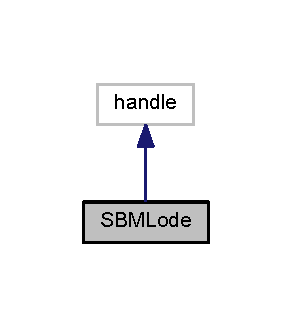
\includegraphics[width=140pt]{class_s_b_m_lode__inherit__graph}
\end{center}
\end{figure}


Collaboration diagram for S\+B\+M\+Lode\+:\nopagebreak
\begin{figure}[H]
\begin{center}
\leavevmode
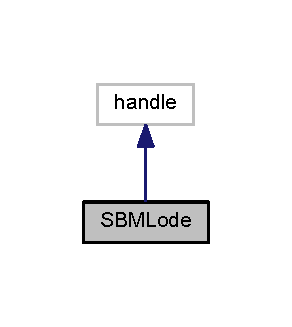
\includegraphics[width=140pt]{class_s_b_m_lode__coll__graph}
\end{center}
\end{figure}
\subsubsection*{Public Member Functions}
\begin{DoxyCompactItemize}
\item 
\hyperlink{class_s_b_m_lode_aafa39f9b845012c546a0e21d38a40582}{S\+B\+M\+Lode} (\+::char filename)
\begin{DoxyCompactList}\small\item\em constructor of the \hyperlink{class_s_b_m_lode}{S\+B\+M\+Lode} class. This takes the name of an S\+B\+M\+L definition file and constructs an \hyperlink{class_s_b_m_lode}{S\+B\+M\+Lode} object based on the parsed model \end{DoxyCompactList}\item 
noret\+::substitute \hyperlink{class_s_b_m_lode_a2265567db5a6aafd85729c20e9d2b631}{import\+S\+B\+M\+L} (matlabtypesubstitute filename)
\begin{DoxyCompactList}\small\item\em import\+S\+B\+M\+L parses the S\+B\+M\+L document and initialises the respective \hyperlink{class_s_b_m_lode}{S\+B\+M\+Lode} object accordingly \end{DoxyCompactList}\item 
noret\+::substitute \hyperlink{class_s_b_m_lode_af2ebf8afc99040060a0af5b3ec3632a7}{write\+A\+M\+I\+C\+I} (matlabtypesubstitute modelname)
\begin{DoxyCompactList}\small\item\em import\+S\+B\+M\+L writes the information stored in the \hyperlink{class_s_b_m_lode}{S\+B\+M\+Lode} object into an A\+M\+I\+C\+I model definition file \end{DoxyCompactList}\end{DoxyCompactItemize}
\subsubsection*{Public Attributes}
\begin{DoxyCompactItemize}
\item 
\+::symbolic \hyperlink{class_s_b_m_lode_adc6e5733fc3c22f0a7b2914188c49c90}{state} = sym(\char`\"{}\mbox{[}$\,$\mbox{]}\char`\"{})
\begin{DoxyCompactList}\small\item\em vector of non-\/constant and non-\/boundary states \end{DoxyCompactList}\item 
\+::symbolic \hyperlink{class_s_b_m_lode_a072b6f6192ac4f40e74b69f901ecdfef}{observable} = sym(\char`\"{}\mbox{[}$\,$\mbox{]}\char`\"{})
\begin{DoxyCompactList}\small\item\em vector of guessed observables \end{DoxyCompactList}\item 
\+::symbolic \hyperlink{class_s_b_m_lode_a6e638e3379dc2d099b3cf3083246fbe0}{observable\+\_\+name} = sym(\char`\"{}\mbox{[}$\,$\mbox{]}\char`\"{})
\begin{DoxyCompactList}\small\item\em vector of guessed observable names \end{DoxyCompactList}\item 
\+::symbolic \hyperlink{class_s_b_m_lode_a51f20d6b1b54a2eee3be0e8adc96a0ae}{param} = sym(\char`\"{}\mbox{[}$\,$\mbox{]}\char`\"{})
\begin{DoxyCompactList}\small\item\em vector of S\+B\+M\+L parameters \end{DoxyCompactList}\item 
\+::symbolic \hyperlink{class_s_b_m_lode_a0d71b5c1dcca8d3fee88d6a11d3e2071}{parameter} = sym(\char`\"{}\mbox{[}$\,$\mbox{]}\char`\"{})
\begin{DoxyCompactList}\small\item\em vector of amimodel parameters \end{DoxyCompactList}\item 
\+::symbolic \hyperlink{class_s_b_m_lode_a391f14c28a859734cd091e4e521bb8f8}{constant} = sym(\char`\"{}\mbox{[}$\,$\mbox{]}\char`\"{})
\begin{DoxyCompactList}\small\item\em vector of constant states \end{DoxyCompactList}\item 
\+::symbolic \hyperlink{class_s_b_m_lode_a70729d905c114f8f08b3507f20806dd2}{compartment} = sym(\char`\"{}\mbox{[}$\,$\mbox{]}\char`\"{})
\begin{DoxyCompactList}\small\item\em vector of compartments \end{DoxyCompactList}\item 
\+::symbolic \hyperlink{class_s_b_m_lode_a9bc498ccac8db41438f855f5dd3f4c05}{volume} = sym(\char`\"{}\mbox{[}$\,$\mbox{]}\char`\"{})
\begin{DoxyCompactList}\small\item\em vector of compartment volumes \end{DoxyCompactList}\item 
\+::symbolic \hyperlink{class_s_b_m_lode_a67d068407e71cba6ca16f3f6b6d1794c}{init\+State} = sym(\char`\"{}\mbox{[}$\,$\mbox{]}\char`\"{})
\begin{DoxyCompactList}\small\item\em vector of initial values for non-\/constant and non-\/boundary states \end{DoxyCompactList}\item 
\+::symbolic \hyperlink{class_s_b_m_lode_a4824b91cc0e6b5f112bdd8049af4d7d6}{condition} = sym(\char`\"{}\mbox{[}$\,$\mbox{]}\char`\"{})
\begin{DoxyCompactList}\small\item\em vector of boundary condition states which are not constant \end{DoxyCompactList}\item 
\+::symbolic \hyperlink{class_s_b_m_lode_a96d7a28b6a4428be15fc1017d19343fa}{flux} = sym(\char`\"{}\mbox{[}$\,$\mbox{]}\char`\"{})
\begin{DoxyCompactList}\small\item\em vector of reaction fluxes \end{DoxyCompactList}\item 
\+::symbolic \hyperlink{class_s_b_m_lode_a8d6dd1568c43b32f1810a5fe9ef6100f}{stochiometry} = sym(\char`\"{}\mbox{[}$\,$\mbox{]}\char`\"{})
\begin{DoxyCompactList}\small\item\em matrix of reaction stochiometries \end{DoxyCompactList}\item 
\+::symbolic \hyperlink{class_s_b_m_lode_a914ee05b8f01d45602316710ca4b8a43}{xdot} = sym(\char`\"{}\mbox{[}$\,$\mbox{]}\char`\"{})
\begin{DoxyCompactList}\small\item\em right hand side of differential equation for states \end{DoxyCompactList}\item 
\+::symbolic \hyperlink{class_s_b_m_lode_ae194cb817eae4085f8023885100c68dd}{trigger} = sym(\char`\"{}\mbox{[}$\,$\mbox{]}\char`\"{})
\begin{DoxyCompactList}\small\item\em vector of trigger functions for events \end{DoxyCompactList}\item 
\+::symbolic \hyperlink{class_s_b_m_lode_ab9227561ac246ee4b70f9e65c25ffda7}{bolus} = sym(\char`\"{}\mbox{[}$\,$\mbox{]}\char`\"{})
\begin{DoxyCompactList}\small\item\em matrix of event bolus \end{DoxyCompactList}\item 
\+::cell \hyperlink{class_s_b_m_lode_a9c1cb6154a226c993c60010300a62e34}{funmath} = \{\char`\"{}\char`\"{}\}
\begin{DoxyCompactList}\small\item\em cell array containing the function definition \end{DoxyCompactList}\item 
\+::cell \hyperlink{class_s_b_m_lode_ae492d28f363cbbf0c960cab4e8911761}{funarg} = \{\char`\"{}\char`\"{}\}
\begin{DoxyCompactList}\small\item\em cell array containing the function arguments \end{DoxyCompactList}\item 
\+::char \hyperlink{class_s_b_m_lode_ac38903669f208bc49c971c7a69f62225}{time\+\_\+symbol} = char(\char`\"{}\mbox{[}$\,$\mbox{]}\char`\"{})
\begin{DoxyCompactList}\small\item\em expression for time in the model \end{DoxyCompactList}\item 
\+::sym \hyperlink{class_s_b_m_lode_aab64bc684d10326610cc4e866d7ed65c}{pnom} = double(\char`\"{}\mbox{[}$\,$\mbox{]}\char`\"{})
\begin{DoxyCompactList}\small\item\em nominal parameter value \end{DoxyCompactList}\item 
\+::sym \hyperlink{class_s_b_m_lode_a744d356a79732f2b65d02f220c580dd4}{knom} = double(\char`\"{}\mbox{[}$\,$\mbox{]}\char`\"{})
\begin{DoxyCompactList}\small\item\em nominal condition value \end{DoxyCompactList}\end{DoxyCompactItemize}


\subsubsection{Detailed Description}


Definition at line 17 of file S\+B\+M\+Lode.\+m.



\subsubsection{Constructor \& Destructor Documentation}
\hypertarget{class_s_b_m_lode_aafa39f9b845012c546a0e21d38a40582}{}\index{S\+B\+M\+Lode@{S\+B\+M\+Lode}!S\+B\+M\+Lode@{S\+B\+M\+Lode}}
\index{S\+B\+M\+Lode@{S\+B\+M\+Lode}!S\+B\+M\+Lode@{S\+B\+M\+Lode}}
\paragraph[{S\+B\+M\+Lode(\+::char filename)}]{\setlength{\rightskip}{0pt plus 5cm}{\bf S\+B\+M\+Lode} (
\begin{DoxyParamCaption}
\item[{\+::char}]{filename}
\end{DoxyParamCaption}
)}\label{class_s_b_m_lode_aafa39f9b845012c546a0e21d38a40582}

\begin{DoxyParams}{Parameters}
{\em filename} & S\+B\+M\+L definition file \\
\hline
\end{DoxyParams}


Definition at line 192 of file S\+B\+M\+Lode.\+m.



\subsubsection{Member Function Documentation}
\hypertarget{class_s_b_m_lode_a2265567db5a6aafd85729c20e9d2b631}{}\index{S\+B\+M\+Lode@{S\+B\+M\+Lode}!import\+S\+B\+M\+L@{import\+S\+B\+M\+L}}
\index{import\+S\+B\+M\+L@{import\+S\+B\+M\+L}!S\+B\+M\+Lode@{S\+B\+M\+Lode}}
\paragraph[{import\+S\+B\+M\+L(matlabtypesubstitute filename)}]{\setlength{\rightskip}{0pt plus 5cm}noret\+::substitute import\+S\+B\+M\+L (
\begin{DoxyParamCaption}
\item[{matlabtypesubstitute}]{modelname}
\end{DoxyParamCaption}
)}\label{class_s_b_m_lode_a2265567db5a6aafd85729c20e9d2b631}

\begin{DoxyParams}{Parameters}
{\em modelname} & name of the sbml model file, without extension\\
\hline
\end{DoxyParams}

\begin{DoxyRetVals}{Return values}
{\em this} & initialised \hyperlink{class_s_b_m_lode}{S\+B\+M\+Lode} object object \\
\hline
\end{DoxyRetVals}


Definition at line 18 of file import\+S\+B\+M\+L.\+m.



Here is the call graph for this function\+:\nopagebreak
\begin{figure}[H]
\begin{center}
\leavevmode
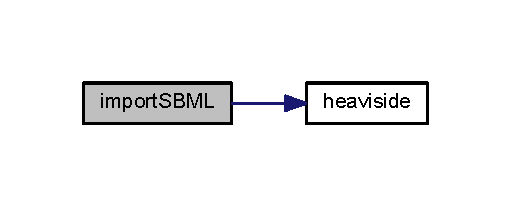
\includegraphics[width=245pt]{class_s_b_m_lode_a2265567db5a6aafd85729c20e9d2b631_cgraph}
\end{center}
\end{figure}


\hypertarget{class_s_b_m_lode_af2ebf8afc99040060a0af5b3ec3632a7}{}\index{S\+B\+M\+Lode@{S\+B\+M\+Lode}!write\+A\+M\+I\+C\+I@{write\+A\+M\+I\+C\+I}}
\index{write\+A\+M\+I\+C\+I@{write\+A\+M\+I\+C\+I}!S\+B\+M\+Lode@{S\+B\+M\+Lode}}
\paragraph[{write\+A\+M\+I\+C\+I(matlabtypesubstitute modelname)}]{\setlength{\rightskip}{0pt plus 5cm}noret\+::substitute write\+A\+M\+I\+C\+I (
\begin{DoxyParamCaption}
\item[{matlabtypesubstitute}]{modelname}
\end{DoxyParamCaption}
)}\label{class_s_b_m_lode_af2ebf8afc99040060a0af5b3ec3632a7}

\begin{DoxyParams}{Parameters}
{\em modelname} & target name of the A\+M\+I\+C\+I model definition file, \+\_\+syms will be appended\\
\hline
\end{DoxyParams}

\begin{DoxyRetVals}{Return values}
{\em this} & initialised \hyperlink{class_s_b_m_lode}{S\+B\+M\+Lode} object object \\
\hline
\end{DoxyRetVals}


Definition at line 18 of file write\+A\+M\+I\+C\+I.\+m.



\subsubsection{Member Data Documentation}
\hypertarget{class_s_b_m_lode_adc6e5733fc3c22f0a7b2914188c49c90}{}\index{S\+B\+M\+Lode@{S\+B\+M\+Lode}!state@{state}}
\index{state@{state}!S\+B\+M\+Lode@{S\+B\+M\+Lode}}
\paragraph[{state}]{\setlength{\rightskip}{0pt plus 5cm}state = sym(\char`\"{}\mbox{[}$\,$\mbox{]}\char`\"{})}\label{class_s_b_m_lode_adc6e5733fc3c22f0a7b2914188c49c90}
~\newline
{\bfseries Default\+:} sym(\char`\"{}\mbox{[}$\,$\mbox{]}\char`\"{}) 

Definition at line 29 of file S\+B\+M\+Lode.\+m.

\hypertarget{class_s_b_m_lode_a072b6f6192ac4f40e74b69f901ecdfef}{}\index{S\+B\+M\+Lode@{S\+B\+M\+Lode}!observable@{observable}}
\index{observable@{observable}!S\+B\+M\+Lode@{S\+B\+M\+Lode}}
\paragraph[{observable}]{\setlength{\rightskip}{0pt plus 5cm}observable = sym(\char`\"{}\mbox{[}$\,$\mbox{]}\char`\"{})}\label{class_s_b_m_lode_a072b6f6192ac4f40e74b69f901ecdfef}
~\newline
{\bfseries Default\+:} sym(\char`\"{}\mbox{[}$\,$\mbox{]}\char`\"{}) 

Definition at line 37 of file S\+B\+M\+Lode.\+m.

\hypertarget{class_s_b_m_lode_a6e638e3379dc2d099b3cf3083246fbe0}{}\index{S\+B\+M\+Lode@{S\+B\+M\+Lode}!observable\+\_\+name@{observable\+\_\+name}}
\index{observable\+\_\+name@{observable\+\_\+name}!S\+B\+M\+Lode@{S\+B\+M\+Lode}}
\paragraph[{observable\+\_\+name}]{\setlength{\rightskip}{0pt plus 5cm}observable\+\_\+name = sym(\char`\"{}\mbox{[}$\,$\mbox{]}\char`\"{})}\label{class_s_b_m_lode_a6e638e3379dc2d099b3cf3083246fbe0}
~\newline
{\bfseries Default\+:} sym(\char`\"{}\mbox{[}$\,$\mbox{]}\char`\"{}) 

Definition at line 45 of file S\+B\+M\+Lode.\+m.

\hypertarget{class_s_b_m_lode_a51f20d6b1b54a2eee3be0e8adc96a0ae}{}\index{S\+B\+M\+Lode@{S\+B\+M\+Lode}!param@{param}}
\index{param@{param}!S\+B\+M\+Lode@{S\+B\+M\+Lode}}
\paragraph[{param}]{\setlength{\rightskip}{0pt plus 5cm}param = sym(\char`\"{}\mbox{[}$\,$\mbox{]}\char`\"{})}\label{class_s_b_m_lode_a51f20d6b1b54a2eee3be0e8adc96a0ae}
~\newline
{\bfseries Default\+:} sym(\char`\"{}\mbox{[}$\,$\mbox{]}\char`\"{}) 

Definition at line 53 of file S\+B\+M\+Lode.\+m.

\hypertarget{class_s_b_m_lode_a0d71b5c1dcca8d3fee88d6a11d3e2071}{}\index{S\+B\+M\+Lode@{S\+B\+M\+Lode}!parameter@{parameter}}
\index{parameter@{parameter}!S\+B\+M\+Lode@{S\+B\+M\+Lode}}
\paragraph[{parameter}]{\setlength{\rightskip}{0pt plus 5cm}parameter = sym(\char`\"{}\mbox{[}$\,$\mbox{]}\char`\"{})}\label{class_s_b_m_lode_a0d71b5c1dcca8d3fee88d6a11d3e2071}
~\newline
{\bfseries Default\+:} sym(\char`\"{}\mbox{[}$\,$\mbox{]}\char`\"{}) 

Definition at line 61 of file S\+B\+M\+Lode.\+m.

\hypertarget{class_s_b_m_lode_a391f14c28a859734cd091e4e521bb8f8}{}\index{S\+B\+M\+Lode@{S\+B\+M\+Lode}!constant@{constant}}
\index{constant@{constant}!S\+B\+M\+Lode@{S\+B\+M\+Lode}}
\paragraph[{constant}]{\setlength{\rightskip}{0pt plus 5cm}constant = sym(\char`\"{}\mbox{[}$\,$\mbox{]}\char`\"{})}\label{class_s_b_m_lode_a391f14c28a859734cd091e4e521bb8f8}
~\newline
{\bfseries Default\+:} sym(\char`\"{}\mbox{[}$\,$\mbox{]}\char`\"{}) 

Definition at line 69 of file S\+B\+M\+Lode.\+m.

\hypertarget{class_s_b_m_lode_a70729d905c114f8f08b3507f20806dd2}{}\index{S\+B\+M\+Lode@{S\+B\+M\+Lode}!compartment@{compartment}}
\index{compartment@{compartment}!S\+B\+M\+Lode@{S\+B\+M\+Lode}}
\paragraph[{compartment}]{\setlength{\rightskip}{0pt plus 5cm}compartment = sym(\char`\"{}\mbox{[}$\,$\mbox{]}\char`\"{})}\label{class_s_b_m_lode_a70729d905c114f8f08b3507f20806dd2}
~\newline
{\bfseries Default\+:} sym(\char`\"{}\mbox{[}$\,$\mbox{]}\char`\"{}) 

Definition at line 77 of file S\+B\+M\+Lode.\+m.

\hypertarget{class_s_b_m_lode_a9bc498ccac8db41438f855f5dd3f4c05}{}\index{S\+B\+M\+Lode@{S\+B\+M\+Lode}!volume@{volume}}
\index{volume@{volume}!S\+B\+M\+Lode@{S\+B\+M\+Lode}}
\paragraph[{volume}]{\setlength{\rightskip}{0pt plus 5cm}volume = sym(\char`\"{}\mbox{[}$\,$\mbox{]}\char`\"{})}\label{class_s_b_m_lode_a9bc498ccac8db41438f855f5dd3f4c05}
~\newline
{\bfseries Default\+:} sym(\char`\"{}\mbox{[}$\,$\mbox{]}\char`\"{}) 

Definition at line 85 of file S\+B\+M\+Lode.\+m.

\hypertarget{class_s_b_m_lode_a67d068407e71cba6ca16f3f6b6d1794c}{}\index{S\+B\+M\+Lode@{S\+B\+M\+Lode}!init\+State@{init\+State}}
\index{init\+State@{init\+State}!S\+B\+M\+Lode@{S\+B\+M\+Lode}}
\paragraph[{init\+State}]{\setlength{\rightskip}{0pt plus 5cm}init\+State = sym(\char`\"{}\mbox{[}$\,$\mbox{]}\char`\"{})}\label{class_s_b_m_lode_a67d068407e71cba6ca16f3f6b6d1794c}
~\newline
{\bfseries Default\+:} sym(\char`\"{}\mbox{[}$\,$\mbox{]}\char`\"{}) 

Definition at line 93 of file S\+B\+M\+Lode.\+m.

\hypertarget{class_s_b_m_lode_a4824b91cc0e6b5f112bdd8049af4d7d6}{}\index{S\+B\+M\+Lode@{S\+B\+M\+Lode}!condition@{condition}}
\index{condition@{condition}!S\+B\+M\+Lode@{S\+B\+M\+Lode}}
\paragraph[{condition}]{\setlength{\rightskip}{0pt plus 5cm}condition = sym(\char`\"{}\mbox{[}$\,$\mbox{]}\char`\"{})}\label{class_s_b_m_lode_a4824b91cc0e6b5f112bdd8049af4d7d6}
~\newline
{\bfseries Default\+:} sym(\char`\"{}\mbox{[}$\,$\mbox{]}\char`\"{}) 

Definition at line 101 of file S\+B\+M\+Lode.\+m.

\hypertarget{class_s_b_m_lode_a96d7a28b6a4428be15fc1017d19343fa}{}\index{S\+B\+M\+Lode@{S\+B\+M\+Lode}!flux@{flux}}
\index{flux@{flux}!S\+B\+M\+Lode@{S\+B\+M\+Lode}}
\paragraph[{flux}]{\setlength{\rightskip}{0pt plus 5cm}flux = sym(\char`\"{}\mbox{[}$\,$\mbox{]}\char`\"{})}\label{class_s_b_m_lode_a96d7a28b6a4428be15fc1017d19343fa}
~\newline
{\bfseries Default\+:} sym(\char`\"{}\mbox{[}$\,$\mbox{]}\char`\"{}) 

Definition at line 109 of file S\+B\+M\+Lode.\+m.

\hypertarget{class_s_b_m_lode_a8d6dd1568c43b32f1810a5fe9ef6100f}{}\index{S\+B\+M\+Lode@{S\+B\+M\+Lode}!stochiometry@{stochiometry}}
\index{stochiometry@{stochiometry}!S\+B\+M\+Lode@{S\+B\+M\+Lode}}
\paragraph[{stochiometry}]{\setlength{\rightskip}{0pt plus 5cm}stochiometry = sym(\char`\"{}\mbox{[}$\,$\mbox{]}\char`\"{})}\label{class_s_b_m_lode_a8d6dd1568c43b32f1810a5fe9ef6100f}
~\newline
{\bfseries Default\+:} sym(\char`\"{}\mbox{[}$\,$\mbox{]}\char`\"{}) 

Definition at line 117 of file S\+B\+M\+Lode.\+m.

\hypertarget{class_s_b_m_lode_a914ee05b8f01d45602316710ca4b8a43}{}\index{S\+B\+M\+Lode@{S\+B\+M\+Lode}!xdot@{xdot}}
\index{xdot@{xdot}!S\+B\+M\+Lode@{S\+B\+M\+Lode}}
\paragraph[{xdot}]{\setlength{\rightskip}{0pt plus 5cm}xdot = sym(\char`\"{}\mbox{[}$\,$\mbox{]}\char`\"{})}\label{class_s_b_m_lode_a914ee05b8f01d45602316710ca4b8a43}
~\newline
{\bfseries Default\+:} sym(\char`\"{}\mbox{[}$\,$\mbox{]}\char`\"{}) 

Definition at line 125 of file S\+B\+M\+Lode.\+m.

\hypertarget{class_s_b_m_lode_ae194cb817eae4085f8023885100c68dd}{}\index{S\+B\+M\+Lode@{S\+B\+M\+Lode}!trigger@{trigger}}
\index{trigger@{trigger}!S\+B\+M\+Lode@{S\+B\+M\+Lode}}
\paragraph[{trigger}]{\setlength{\rightskip}{0pt plus 5cm}trigger = sym(\char`\"{}\mbox{[}$\,$\mbox{]}\char`\"{})}\label{class_s_b_m_lode_ae194cb817eae4085f8023885100c68dd}
~\newline
{\bfseries Default\+:} sym(\char`\"{}\mbox{[}$\,$\mbox{]}\char`\"{}) 

Definition at line 133 of file S\+B\+M\+Lode.\+m.

\hypertarget{class_s_b_m_lode_ab9227561ac246ee4b70f9e65c25ffda7}{}\index{S\+B\+M\+Lode@{S\+B\+M\+Lode}!bolus@{bolus}}
\index{bolus@{bolus}!S\+B\+M\+Lode@{S\+B\+M\+Lode}}
\paragraph[{bolus}]{\setlength{\rightskip}{0pt plus 5cm}bolus = sym(\char`\"{}\mbox{[}$\,$\mbox{]}\char`\"{})}\label{class_s_b_m_lode_ab9227561ac246ee4b70f9e65c25ffda7}
~\newline
{\bfseries Default\+:} sym(\char`\"{}\mbox{[}$\,$\mbox{]}\char`\"{}) 

Definition at line 141 of file S\+B\+M\+Lode.\+m.

\hypertarget{class_s_b_m_lode_a9c1cb6154a226c993c60010300a62e34}{}\index{S\+B\+M\+Lode@{S\+B\+M\+Lode}!funmath@{funmath}}
\index{funmath@{funmath}!S\+B\+M\+Lode@{S\+B\+M\+Lode}}
\paragraph[{funmath}]{\setlength{\rightskip}{0pt plus 5cm}funmath = \{\char`\"{}\char`\"{}\}}\label{class_s_b_m_lode_a9c1cb6154a226c993c60010300a62e34}
~\newline
{\bfseries Default\+:} \{\char`\"{}\char`\"{}\} 

Definition at line 149 of file S\+B\+M\+Lode.\+m.

\hypertarget{class_s_b_m_lode_ae492d28f363cbbf0c960cab4e8911761}{}\index{S\+B\+M\+Lode@{S\+B\+M\+Lode}!funarg@{funarg}}
\index{funarg@{funarg}!S\+B\+M\+Lode@{S\+B\+M\+Lode}}
\paragraph[{funarg}]{\setlength{\rightskip}{0pt plus 5cm}funarg = \{\char`\"{}\char`\"{}\}}\label{class_s_b_m_lode_ae492d28f363cbbf0c960cab4e8911761}
~\newline
{\bfseries Default\+:} \{\char`\"{}\char`\"{}\} 

Definition at line 157 of file S\+B\+M\+Lode.\+m.

\hypertarget{class_s_b_m_lode_ac38903669f208bc49c971c7a69f62225}{}\index{S\+B\+M\+Lode@{S\+B\+M\+Lode}!time\+\_\+symbol@{time\+\_\+symbol}}
\index{time\+\_\+symbol@{time\+\_\+symbol}!S\+B\+M\+Lode@{S\+B\+M\+Lode}}
\paragraph[{time\+\_\+symbol}]{\setlength{\rightskip}{0pt plus 5cm}time\+\_\+symbol = char(\char`\"{}\mbox{[}$\,$\mbox{]}\char`\"{})}\label{class_s_b_m_lode_ac38903669f208bc49c971c7a69f62225}
~\newline
{\bfseries Default\+:} char(\char`\"{}\mbox{[}$\,$\mbox{]}\char`\"{}) 

Definition at line 165 of file S\+B\+M\+Lode.\+m.

\hypertarget{class_s_b_m_lode_aab64bc684d10326610cc4e866d7ed65c}{}\index{S\+B\+M\+Lode@{S\+B\+M\+Lode}!pnom@{pnom}}
\index{pnom@{pnom}!S\+B\+M\+Lode@{S\+B\+M\+Lode}}
\paragraph[{pnom}]{\setlength{\rightskip}{0pt plus 5cm}pnom = double(\char`\"{}\mbox{[}$\,$\mbox{]}\char`\"{})}\label{class_s_b_m_lode_aab64bc684d10326610cc4e866d7ed65c}
~\newline
{\bfseries Default\+:} double(\char`\"{}\mbox{[}$\,$\mbox{]}\char`\"{}) 

Definition at line 173 of file S\+B\+M\+Lode.\+m.

\hypertarget{class_s_b_m_lode_a744d356a79732f2b65d02f220c580dd4}{}\index{S\+B\+M\+Lode@{S\+B\+M\+Lode}!knom@{knom}}
\index{knom@{knom}!S\+B\+M\+Lode@{S\+B\+M\+Lode}}
\paragraph[{knom}]{\setlength{\rightskip}{0pt plus 5cm}knom = double(\char`\"{}\mbox{[}$\,$\mbox{]}\char`\"{})}\label{class_s_b_m_lode_a744d356a79732f2b65d02f220c580dd4}
~\newline
{\bfseries Default\+:} double(\char`\"{}\mbox{[}$\,$\mbox{]}\char`\"{}) 

Definition at line 181 of file S\+B\+M\+Lode.\+m.


\hypertarget{struct_temp_data}{}\subsection{Temp\+Data Struct Reference}
\label{struct_temp_data}\index{Temp\+Data@{Temp\+Data}}


struct that provides temporary storage for different variables  




{\ttfamily \#include $<$tdata.\+h$>$}

\subsubsection*{Public Attributes}
\begin{DoxyCompactItemize}
\item 
realtype \hyperlink{struct_temp_data_ae0484650df254ad9cd8883e2ba028892}{am\+\_\+t}
\item 
N\+\_\+\+Vector \hyperlink{struct_temp_data_a4527d9abde45ba3982c35d2c12969d36}{am\+\_\+x}
\item 
N\+\_\+\+Vector \hyperlink{struct_temp_data_ab2b23f4045b47a4a73226543e77f9dcc}{am\+\_\+x\+\_\+old}
\item 
N\+\_\+\+Vector $\ast$ \hyperlink{struct_temp_data_aded6511f60d9b0cdfe5f4df047d8a5dd}{am\+\_\+x\+\_\+disc}
\item 
N\+\_\+\+Vector $\ast$ \hyperlink{struct_temp_data_ab3837be5f66a858b04b2e6fbae66a100}{am\+\_\+xdot\+\_\+disc}
\item 
N\+\_\+\+Vector $\ast$ \hyperlink{struct_temp_data_aae23888e89a7bd3c65a22784acaa1328}{am\+\_\+xdot\+\_\+old\+\_\+disc}
\item 
N\+\_\+\+Vector \hyperlink{struct_temp_data_ac10ec733609d33c557d48c1cc4c9f6f1}{am\+\_\+dx}
\item 
N\+\_\+\+Vector \hyperlink{struct_temp_data_aca2465f16eeb5dc94cea61c970f2682a}{am\+\_\+dx\+\_\+old}
\item 
N\+\_\+\+Vector \hyperlink{struct_temp_data_abad4a9e3cc9cd42b3fe4e2fe28a915c1}{am\+\_\+xdot}
\item 
N\+\_\+\+Vector \hyperlink{struct_temp_data_a6a8af565a7f6ec58c4fbcd044c049d80}{am\+\_\+xdot\+\_\+old}
\item 
N\+\_\+\+Vector \hyperlink{struct_temp_data_a318f0b9b1f4b33326184a350912c6fb1}{am\+\_\+x\+B}
\item 
N\+\_\+\+Vector \hyperlink{struct_temp_data_a33e09af3351a4d4889e62d0d0d964ce5}{am\+\_\+x\+B\+\_\+old}
\item 
N\+\_\+\+Vector \hyperlink{struct_temp_data_a6dc87d123304fe3c6a20899fca777501}{am\+\_\+dx\+B}
\item 
N\+\_\+\+Vector \hyperlink{struct_temp_data_ac4099b4f6bf1f15d7d07b88993515da7}{am\+\_\+x\+Q\+B}
\item 
N\+\_\+\+Vector \hyperlink{struct_temp_data_a132a821ce32c806eb4691a94da216e29}{am\+\_\+x\+Q\+B\+\_\+old}
\item 
N\+\_\+\+Vector $\ast$ \hyperlink{struct_temp_data_a5253085927038bdeb7c327aa14470722}{am\+\_\+sx}
\item 
N\+\_\+\+Vector $\ast$ \hyperlink{struct_temp_data_a2457438c1ae3ea571031bc3c2e440da2}{am\+\_\+sdx}
\item 
N\+\_\+\+Vector \hyperlink{struct_temp_data_ad918917fdce710fbd6fe9774e35bfcfb}{am\+\_\+id}
\item 
Dls\+Mat \hyperlink{struct_temp_data_aa850cd4b6b24d0b98b4aac8f42a057a1}{am\+\_\+\+Jtmp}
\item 
realtype $\ast$ \hyperlink{struct_temp_data_ac8e571186f15f3172f69d2e016023fbc}{am\+\_\+llh\+S0}
\item 
realtype \hyperlink{struct_temp_data_abcec297db6f0e216e479c6f4f2cdb5ff}{am\+\_\+g}
\item 
realtype $\ast$ \hyperlink{struct_temp_data_a081b11391c89402abac604021f6ccf9d}{am\+\_\+dgdp}
\item 
realtype $\ast$ \hyperlink{struct_temp_data_ae858332947a50294436a0bbf2b7a8ea1}{am\+\_\+dgdx}
\item 
realtype \hyperlink{struct_temp_data_a7f00edd52d15fce2def96917a9ee47dc}{am\+\_\+r}
\item 
realtype $\ast$ \hyperlink{struct_temp_data_ab9c815d99f44f36f068133746323b5cc}{am\+\_\+drdp}
\item 
realtype $\ast$ \hyperlink{struct_temp_data_a92cb58d44aef5760bf9ad22690e48113}{am\+\_\+drdx}
\item 
realtype \hyperlink{struct_temp_data_abf2c3d254f311ab4385f18cff8acb89a}{am\+\_\+rval}
\item 
realtype $\ast$ \hyperlink{struct_temp_data_af51ded83b415e8a9d8e4f67736d11d34}{am\+\_\+drvaldp}
\item 
realtype $\ast$ \hyperlink{struct_temp_data_ae474fa93074514dd5b9d6ef00aa7345d}{am\+\_\+drvaldx}
\item 
realtype $\ast$ \hyperlink{struct_temp_data_a9309d8a421155cac9ad1c3fd1b5b0f56}{am\+\_\+dzdx}
\item 
realtype $\ast$ \hyperlink{struct_temp_data_a1df093f48bf98db04c63e845d7b1d58b}{am\+\_\+dzdp}
\item 
realtype $\ast$ \hyperlink{struct_temp_data_a76083cb4a9598daa381dbaa9c17aadc6}{am\+\_\+dydp}
\item 
realtype $\ast$ \hyperlink{struct_temp_data_a062c7ecfd4107b320dfd2fc0e4211a6b}{am\+\_\+dydx}
\item 
realtype $\ast$ \hyperlink{struct_temp_data_a7c1a4e54905d0fea6c4ec952cd7a96d8}{am\+\_\+y\+S0}
\item 
realtype $\ast$ \hyperlink{struct_temp_data_ac152c0012fafda7a5ec5f2163eebfcda}{am\+\_\+sigma\+\_\+y}
\item 
realtype $\ast$ \hyperlink{struct_temp_data_a27781d18ccc799ac0074d2dc39d51abc}{am\+\_\+dsigma\+\_\+ydp}
\item 
realtype $\ast$ \hyperlink{struct_temp_data_a6326bdfdde6ff9d3e52a80760e403a02}{am\+\_\+sigma\+\_\+z}
\item 
realtype $\ast$ \hyperlink{struct_temp_data_ad918e459ea613f39e2d2a2fe62b68137}{am\+\_\+dsigma\+\_\+zdp}
\item 
realtype $\ast$ \hyperlink{struct_temp_data_a7751aebb2b290fc4a51d9ca5f47fb455}{am\+\_\+x\+\_\+tmp}
\item 
realtype $\ast$ \hyperlink{struct_temp_data_a4b0bde10a390f324386b07acacd367bc}{am\+\_\+sx\+\_\+tmp}
\item 
realtype $\ast$ \hyperlink{struct_temp_data_abd683baa60bb69c9731961ba50e1455d}{am\+\_\+dx\+\_\+tmp}
\item 
realtype $\ast$ \hyperlink{struct_temp_data_ac0bc306224fbe129accbc959efda5451}{am\+\_\+sdx\+\_\+tmp}
\item 
realtype $\ast$ \hyperlink{struct_temp_data_ac28b5a5a19ad2004d32d20098d3603ed}{am\+\_\+xdot\+\_\+tmp}
\item 
realtype $\ast$ \hyperlink{struct_temp_data_a71147dc6b9970cafbada503f873d0dfe}{am\+\_\+x\+B\+\_\+tmp}
\item 
realtype $\ast$ \hyperlink{struct_temp_data_a18e2184588648670c2df22856f441e32}{am\+\_\+x\+Q\+B\+\_\+tmp}
\item 
realtype $\ast$ \hyperlink{struct_temp_data_a147fbb5ac85bc9ce0f55cb9108663e1b}{am\+\_\+dx\+B\+\_\+tmp}
\item 
realtype $\ast$ \hyperlink{struct_temp_data_af4cb4bb8ec3396d46cca992ad83ae137}{am\+\_\+id\+\_\+tmp}
\item 
int $\ast$ \hyperlink{struct_temp_data_a7aead84117fd84087a23d968ea56b542}{am\+\_\+rootsfound}
\item 
int $\ast$ \hyperlink{struct_temp_data_a360ea220e712750c92bd3fc8b56230e2}{am\+\_\+rootidx}
\item 
int $\ast$ \hyperlink{struct_temp_data_af329293bdb28f52dcaeb04355dc5c69e}{am\+\_\+nroots}
\item 
double $\ast$ \hyperlink{struct_temp_data_a9cf09c47af8f82be3bba711720009efe}{am\+\_\+rootvals}
\item 
realtype $\ast$ \hyperlink{struct_temp_data_ab432281618cfe0f7dd7db1d8eb5ec227}{am\+\_\+deltax}
\item 
realtype $\ast$ \hyperlink{struct_temp_data_a96e5e38eb662e4b1390a14693e17ece5}{am\+\_\+deltasx}
\item 
realtype $\ast$ \hyperlink{struct_temp_data_a75047d78cee16ec77b9aae2cf0a25964}{am\+\_\+deltax\+B}
\item 
realtype $\ast$ \hyperlink{struct_temp_data_adfe8df7debe43dd76c29e4976b1f1ae7}{am\+\_\+deltaq\+B}
\item 
int \hyperlink{struct_temp_data_a961819e25ceef7e842c469cbedccb19f}{am\+\_\+which}
\item 
realtype $\ast$ \hyperlink{struct_temp_data_aeb8b1beb27f1b20bda3d7de494f58c41}{am\+\_\+discs}
\item 
realtype $\ast$ \hyperlink{struct_temp_data_ad64693949a923975059d0d0c49e854f9}{am\+\_\+irdiscs}
\end{DoxyCompactItemize}


\subsubsection{Detailed Description}


Definition at line 78 of file tdata.\+h.



\subsubsection{Member Data Documentation}
\hypertarget{struct_temp_data_ae0484650df254ad9cd8883e2ba028892}{}\index{Temp\+Data@{Temp\+Data}!am\+\_\+t@{am\+\_\+t}}
\index{am\+\_\+t@{am\+\_\+t}!Temp\+Data@{Temp\+Data}}
\paragraph[{am\+\_\+t}]{\setlength{\rightskip}{0pt plus 5cm}realtype am\+\_\+t}\label{struct_temp_data_ae0484650df254ad9cd8883e2ba028892}
current time 

Definition at line 80 of file tdata.\+h.

\hypertarget{struct_temp_data_a4527d9abde45ba3982c35d2c12969d36}{}\index{Temp\+Data@{Temp\+Data}!am\+\_\+x@{am\+\_\+x}}
\index{am\+\_\+x@{am\+\_\+x}!Temp\+Data@{Temp\+Data}}
\paragraph[{am\+\_\+x}]{\setlength{\rightskip}{0pt plus 5cm}N\+\_\+\+Vector am\+\_\+x}\label{struct_temp_data_a4527d9abde45ba3982c35d2c12969d36}
state vector 

Definition at line 84 of file tdata.\+h.

\hypertarget{struct_temp_data_ab2b23f4045b47a4a73226543e77f9dcc}{}\index{Temp\+Data@{Temp\+Data}!am\+\_\+x\+\_\+old@{am\+\_\+x\+\_\+old}}
\index{am\+\_\+x\+\_\+old@{am\+\_\+x\+\_\+old}!Temp\+Data@{Temp\+Data}}
\paragraph[{am\+\_\+x\+\_\+old}]{\setlength{\rightskip}{0pt plus 5cm}N\+\_\+\+Vector am\+\_\+x\+\_\+old}\label{struct_temp_data_ab2b23f4045b47a4a73226543e77f9dcc}
old state vector 

Definition at line 86 of file tdata.\+h.

\hypertarget{struct_temp_data_aded6511f60d9b0cdfe5f4df047d8a5dd}{}\index{Temp\+Data@{Temp\+Data}!am\+\_\+x\+\_\+disc@{am\+\_\+x\+\_\+disc}}
\index{am\+\_\+x\+\_\+disc@{am\+\_\+x\+\_\+disc}!Temp\+Data@{Temp\+Data}}
\paragraph[{am\+\_\+x\+\_\+disc}]{\setlength{\rightskip}{0pt plus 5cm}N\+\_\+\+Vector$\ast$ am\+\_\+x\+\_\+disc}\label{struct_temp_data_aded6511f60d9b0cdfe5f4df047d8a5dd}
array of state vectors at discontinuities 

Definition at line 88 of file tdata.\+h.

\hypertarget{struct_temp_data_ab3837be5f66a858b04b2e6fbae66a100}{}\index{Temp\+Data@{Temp\+Data}!am\+\_\+xdot\+\_\+disc@{am\+\_\+xdot\+\_\+disc}}
\index{am\+\_\+xdot\+\_\+disc@{am\+\_\+xdot\+\_\+disc}!Temp\+Data@{Temp\+Data}}
\paragraph[{am\+\_\+xdot\+\_\+disc}]{\setlength{\rightskip}{0pt plus 5cm}N\+\_\+\+Vector$\ast$ am\+\_\+xdot\+\_\+disc}\label{struct_temp_data_ab3837be5f66a858b04b2e6fbae66a100}
array of differential state vectors at discontinuities 

Definition at line 90 of file tdata.\+h.

\hypertarget{struct_temp_data_aae23888e89a7bd3c65a22784acaa1328}{}\index{Temp\+Data@{Temp\+Data}!am\+\_\+xdot\+\_\+old\+\_\+disc@{am\+\_\+xdot\+\_\+old\+\_\+disc}}
\index{am\+\_\+xdot\+\_\+old\+\_\+disc@{am\+\_\+xdot\+\_\+old\+\_\+disc}!Temp\+Data@{Temp\+Data}}
\paragraph[{am\+\_\+xdot\+\_\+old\+\_\+disc}]{\setlength{\rightskip}{0pt plus 5cm}N\+\_\+\+Vector$\ast$ am\+\_\+xdot\+\_\+old\+\_\+disc}\label{struct_temp_data_aae23888e89a7bd3c65a22784acaa1328}
array of old differential state vectors at discontinuities 

Definition at line 92 of file tdata.\+h.

\hypertarget{struct_temp_data_ac10ec733609d33c557d48c1cc4c9f6f1}{}\index{Temp\+Data@{Temp\+Data}!am\+\_\+dx@{am\+\_\+dx}}
\index{am\+\_\+dx@{am\+\_\+dx}!Temp\+Data@{Temp\+Data}}
\paragraph[{am\+\_\+dx}]{\setlength{\rightskip}{0pt plus 5cm}N\+\_\+\+Vector am\+\_\+dx}\label{struct_temp_data_ac10ec733609d33c557d48c1cc4c9f6f1}
differential state vector 

Definition at line 94 of file tdata.\+h.

\hypertarget{struct_temp_data_aca2465f16eeb5dc94cea61c970f2682a}{}\index{Temp\+Data@{Temp\+Data}!am\+\_\+dx\+\_\+old@{am\+\_\+dx\+\_\+old}}
\index{am\+\_\+dx\+\_\+old@{am\+\_\+dx\+\_\+old}!Temp\+Data@{Temp\+Data}}
\paragraph[{am\+\_\+dx\+\_\+old}]{\setlength{\rightskip}{0pt plus 5cm}N\+\_\+\+Vector am\+\_\+dx\+\_\+old}\label{struct_temp_data_aca2465f16eeb5dc94cea61c970f2682a}
old differential state vector 

Definition at line 96 of file tdata.\+h.

\hypertarget{struct_temp_data_abad4a9e3cc9cd42b3fe4e2fe28a915c1}{}\index{Temp\+Data@{Temp\+Data}!am\+\_\+xdot@{am\+\_\+xdot}}
\index{am\+\_\+xdot@{am\+\_\+xdot}!Temp\+Data@{Temp\+Data}}
\paragraph[{am\+\_\+xdot}]{\setlength{\rightskip}{0pt plus 5cm}N\+\_\+\+Vector am\+\_\+xdot}\label{struct_temp_data_abad4a9e3cc9cd42b3fe4e2fe28a915c1}
time derivative state vector 

Definition at line 98 of file tdata.\+h.

\hypertarget{struct_temp_data_a6a8af565a7f6ec58c4fbcd044c049d80}{}\index{Temp\+Data@{Temp\+Data}!am\+\_\+xdot\+\_\+old@{am\+\_\+xdot\+\_\+old}}
\index{am\+\_\+xdot\+\_\+old@{am\+\_\+xdot\+\_\+old}!Temp\+Data@{Temp\+Data}}
\paragraph[{am\+\_\+xdot\+\_\+old}]{\setlength{\rightskip}{0pt plus 5cm}N\+\_\+\+Vector am\+\_\+xdot\+\_\+old}\label{struct_temp_data_a6a8af565a7f6ec58c4fbcd044c049d80}
old time derivative state vector 

Definition at line 100 of file tdata.\+h.

\hypertarget{struct_temp_data_a318f0b9b1f4b33326184a350912c6fb1}{}\index{Temp\+Data@{Temp\+Data}!am\+\_\+x\+B@{am\+\_\+x\+B}}
\index{am\+\_\+x\+B@{am\+\_\+x\+B}!Temp\+Data@{Temp\+Data}}
\paragraph[{am\+\_\+x\+B}]{\setlength{\rightskip}{0pt plus 5cm}N\+\_\+\+Vector am\+\_\+x\+B}\label{struct_temp_data_a318f0b9b1f4b33326184a350912c6fb1}
adjoint state vector 

Definition at line 102 of file tdata.\+h.

\hypertarget{struct_temp_data_a33e09af3351a4d4889e62d0d0d964ce5}{}\index{Temp\+Data@{Temp\+Data}!am\+\_\+x\+B\+\_\+old@{am\+\_\+x\+B\+\_\+old}}
\index{am\+\_\+x\+B\+\_\+old@{am\+\_\+x\+B\+\_\+old}!Temp\+Data@{Temp\+Data}}
\paragraph[{am\+\_\+x\+B\+\_\+old}]{\setlength{\rightskip}{0pt plus 5cm}N\+\_\+\+Vector am\+\_\+x\+B\+\_\+old}\label{struct_temp_data_a33e09af3351a4d4889e62d0d0d964ce5}
old adjoint state vector 

Definition at line 104 of file tdata.\+h.

\hypertarget{struct_temp_data_a6dc87d123304fe3c6a20899fca777501}{}\index{Temp\+Data@{Temp\+Data}!am\+\_\+dx\+B@{am\+\_\+dx\+B}}
\index{am\+\_\+dx\+B@{am\+\_\+dx\+B}!Temp\+Data@{Temp\+Data}}
\paragraph[{am\+\_\+dx\+B}]{\setlength{\rightskip}{0pt plus 5cm}N\+\_\+\+Vector am\+\_\+dx\+B}\label{struct_temp_data_a6dc87d123304fe3c6a20899fca777501}
differential adjoint state vector 

Definition at line 106 of file tdata.\+h.

\hypertarget{struct_temp_data_ac4099b4f6bf1f15d7d07b88993515da7}{}\index{Temp\+Data@{Temp\+Data}!am\+\_\+x\+Q\+B@{am\+\_\+x\+Q\+B}}
\index{am\+\_\+x\+Q\+B@{am\+\_\+x\+Q\+B}!Temp\+Data@{Temp\+Data}}
\paragraph[{am\+\_\+x\+Q\+B}]{\setlength{\rightskip}{0pt plus 5cm}N\+\_\+\+Vector am\+\_\+x\+Q\+B}\label{struct_temp_data_ac4099b4f6bf1f15d7d07b88993515da7}
quadrature state vector 

Definition at line 108 of file tdata.\+h.

\hypertarget{struct_temp_data_a132a821ce32c806eb4691a94da216e29}{}\index{Temp\+Data@{Temp\+Data}!am\+\_\+x\+Q\+B\+\_\+old@{am\+\_\+x\+Q\+B\+\_\+old}}
\index{am\+\_\+x\+Q\+B\+\_\+old@{am\+\_\+x\+Q\+B\+\_\+old}!Temp\+Data@{Temp\+Data}}
\paragraph[{am\+\_\+x\+Q\+B\+\_\+old}]{\setlength{\rightskip}{0pt plus 5cm}N\+\_\+\+Vector am\+\_\+x\+Q\+B\+\_\+old}\label{struct_temp_data_a132a821ce32c806eb4691a94da216e29}
old quadrature state vector 

Definition at line 110 of file tdata.\+h.

\hypertarget{struct_temp_data_a5253085927038bdeb7c327aa14470722}{}\index{Temp\+Data@{Temp\+Data}!am\+\_\+sx@{am\+\_\+sx}}
\index{am\+\_\+sx@{am\+\_\+sx}!Temp\+Data@{Temp\+Data}}
\paragraph[{am\+\_\+sx}]{\setlength{\rightskip}{0pt plus 5cm}N\+\_\+\+Vector$\ast$ am\+\_\+sx}\label{struct_temp_data_a5253085927038bdeb7c327aa14470722}
sensitivity state vector array 

Definition at line 112 of file tdata.\+h.

\hypertarget{struct_temp_data_a2457438c1ae3ea571031bc3c2e440da2}{}\index{Temp\+Data@{Temp\+Data}!am\+\_\+sdx@{am\+\_\+sdx}}
\index{am\+\_\+sdx@{am\+\_\+sdx}!Temp\+Data@{Temp\+Data}}
\paragraph[{am\+\_\+sdx}]{\setlength{\rightskip}{0pt plus 5cm}N\+\_\+\+Vector$\ast$ am\+\_\+sdx}\label{struct_temp_data_a2457438c1ae3ea571031bc3c2e440da2}
differential sensitivity state vector array 

Definition at line 114 of file tdata.\+h.

\hypertarget{struct_temp_data_ad918917fdce710fbd6fe9774e35bfcfb}{}\index{Temp\+Data@{Temp\+Data}!am\+\_\+id@{am\+\_\+id}}
\index{am\+\_\+id@{am\+\_\+id}!Temp\+Data@{Temp\+Data}}
\paragraph[{am\+\_\+id}]{\setlength{\rightskip}{0pt plus 5cm}N\+\_\+\+Vector am\+\_\+id}\label{struct_temp_data_ad918917fdce710fbd6fe9774e35bfcfb}
index indicating D\+A\+E equations vector 

Definition at line 116 of file tdata.\+h.

\hypertarget{struct_temp_data_aa850cd4b6b24d0b98b4aac8f42a057a1}{}\index{Temp\+Data@{Temp\+Data}!am\+\_\+\+Jtmp@{am\+\_\+\+Jtmp}}
\index{am\+\_\+\+Jtmp@{am\+\_\+\+Jtmp}!Temp\+Data@{Temp\+Data}}
\paragraph[{am\+\_\+\+Jtmp}]{\setlength{\rightskip}{0pt plus 5cm}Dls\+Mat am\+\_\+\+Jtmp}\label{struct_temp_data_aa850cd4b6b24d0b98b4aac8f42a057a1}
Jacobian 

Definition at line 118 of file tdata.\+h.

\hypertarget{struct_temp_data_ac8e571186f15f3172f69d2e016023fbc}{}\index{Temp\+Data@{Temp\+Data}!am\+\_\+llh\+S0@{am\+\_\+llh\+S0}}
\index{am\+\_\+llh\+S0@{am\+\_\+llh\+S0}!Temp\+Data@{Temp\+Data}}
\paragraph[{am\+\_\+llh\+S0}]{\setlength{\rightskip}{0pt plus 5cm}realtype$\ast$ am\+\_\+llh\+S0}\label{struct_temp_data_ac8e571186f15f3172f69d2e016023fbc}
parameter derivative of likelihood array 

Definition at line 121 of file tdata.\+h.

\hypertarget{struct_temp_data_abcec297db6f0e216e479c6f4f2cdb5ff}{}\index{Temp\+Data@{Temp\+Data}!am\+\_\+g@{am\+\_\+g}}
\index{am\+\_\+g@{am\+\_\+g}!Temp\+Data@{Temp\+Data}}
\paragraph[{am\+\_\+g}]{\setlength{\rightskip}{0pt plus 5cm}realtype am\+\_\+g}\label{struct_temp_data_abcec297db6f0e216e479c6f4f2cdb5ff}
data likelihood 

Definition at line 123 of file tdata.\+h.

\hypertarget{struct_temp_data_a081b11391c89402abac604021f6ccf9d}{}\index{Temp\+Data@{Temp\+Data}!am\+\_\+dgdp@{am\+\_\+dgdp}}
\index{am\+\_\+dgdp@{am\+\_\+dgdp}!Temp\+Data@{Temp\+Data}}
\paragraph[{am\+\_\+dgdp}]{\setlength{\rightskip}{0pt plus 5cm}realtype$\ast$ am\+\_\+dgdp}\label{struct_temp_data_a081b11391c89402abac604021f6ccf9d}
parameter derivative of data likelihood 

Definition at line 125 of file tdata.\+h.

\hypertarget{struct_temp_data_ae858332947a50294436a0bbf2b7a8ea1}{}\index{Temp\+Data@{Temp\+Data}!am\+\_\+dgdx@{am\+\_\+dgdx}}
\index{am\+\_\+dgdx@{am\+\_\+dgdx}!Temp\+Data@{Temp\+Data}}
\paragraph[{am\+\_\+dgdx}]{\setlength{\rightskip}{0pt plus 5cm}realtype$\ast$ am\+\_\+dgdx}\label{struct_temp_data_ae858332947a50294436a0bbf2b7a8ea1}
state derivative of data likelihood 

Definition at line 127 of file tdata.\+h.

\hypertarget{struct_temp_data_a7f00edd52d15fce2def96917a9ee47dc}{}\index{Temp\+Data@{Temp\+Data}!am\+\_\+r@{am\+\_\+r}}
\index{am\+\_\+r@{am\+\_\+r}!Temp\+Data@{Temp\+Data}}
\paragraph[{am\+\_\+r}]{\setlength{\rightskip}{0pt plus 5cm}realtype am\+\_\+r}\label{struct_temp_data_a7f00edd52d15fce2def96917a9ee47dc}
event likelihood 

Definition at line 129 of file tdata.\+h.

\hypertarget{struct_temp_data_ab9c815d99f44f36f068133746323b5cc}{}\index{Temp\+Data@{Temp\+Data}!am\+\_\+drdp@{am\+\_\+drdp}}
\index{am\+\_\+drdp@{am\+\_\+drdp}!Temp\+Data@{Temp\+Data}}
\paragraph[{am\+\_\+drdp}]{\setlength{\rightskip}{0pt plus 5cm}realtype$\ast$ am\+\_\+drdp}\label{struct_temp_data_ab9c815d99f44f36f068133746323b5cc}
parameter derivative of event likelihood 

Definition at line 131 of file tdata.\+h.

\hypertarget{struct_temp_data_a92cb58d44aef5760bf9ad22690e48113}{}\index{Temp\+Data@{Temp\+Data}!am\+\_\+drdx@{am\+\_\+drdx}}
\index{am\+\_\+drdx@{am\+\_\+drdx}!Temp\+Data@{Temp\+Data}}
\paragraph[{am\+\_\+drdx}]{\setlength{\rightskip}{0pt plus 5cm}realtype$\ast$ am\+\_\+drdx}\label{struct_temp_data_a92cb58d44aef5760bf9ad22690e48113}
state derivative of event likelihood 

Definition at line 133 of file tdata.\+h.

\hypertarget{struct_temp_data_abf2c3d254f311ab4385f18cff8acb89a}{}\index{Temp\+Data@{Temp\+Data}!am\+\_\+rval@{am\+\_\+rval}}
\index{am\+\_\+rval@{am\+\_\+rval}!Temp\+Data@{Temp\+Data}}
\paragraph[{am\+\_\+rval}]{\setlength{\rightskip}{0pt plus 5cm}realtype am\+\_\+rval}\label{struct_temp_data_abf2c3d254f311ab4385f18cff8acb89a}
root function likelihood 

Definition at line 135 of file tdata.\+h.

\hypertarget{struct_temp_data_af51ded83b415e8a9d8e4f67736d11d34}{}\index{Temp\+Data@{Temp\+Data}!am\+\_\+drvaldp@{am\+\_\+drvaldp}}
\index{am\+\_\+drvaldp@{am\+\_\+drvaldp}!Temp\+Data@{Temp\+Data}}
\paragraph[{am\+\_\+drvaldp}]{\setlength{\rightskip}{0pt plus 5cm}realtype$\ast$ am\+\_\+drvaldp}\label{struct_temp_data_af51ded83b415e8a9d8e4f67736d11d34}
parameter derivative of root function likelihood 

Definition at line 137 of file tdata.\+h.

\hypertarget{struct_temp_data_ae474fa93074514dd5b9d6ef00aa7345d}{}\index{Temp\+Data@{Temp\+Data}!am\+\_\+drvaldx@{am\+\_\+drvaldx}}
\index{am\+\_\+drvaldx@{am\+\_\+drvaldx}!Temp\+Data@{Temp\+Data}}
\paragraph[{am\+\_\+drvaldx}]{\setlength{\rightskip}{0pt plus 5cm}realtype$\ast$ am\+\_\+drvaldx}\label{struct_temp_data_ae474fa93074514dd5b9d6ef00aa7345d}
state derivative of root function likelihood 

Definition at line 139 of file tdata.\+h.

\hypertarget{struct_temp_data_a9309d8a421155cac9ad1c3fd1b5b0f56}{}\index{Temp\+Data@{Temp\+Data}!am\+\_\+dzdx@{am\+\_\+dzdx}}
\index{am\+\_\+dzdx@{am\+\_\+dzdx}!Temp\+Data@{Temp\+Data}}
\paragraph[{am\+\_\+dzdx}]{\setlength{\rightskip}{0pt plus 5cm}realtype$\ast$ am\+\_\+dzdx}\label{struct_temp_data_a9309d8a421155cac9ad1c3fd1b5b0f56}
state derivative of event 

Definition at line 141 of file tdata.\+h.

\hypertarget{struct_temp_data_a1df093f48bf98db04c63e845d7b1d58b}{}\index{Temp\+Data@{Temp\+Data}!am\+\_\+dzdp@{am\+\_\+dzdp}}
\index{am\+\_\+dzdp@{am\+\_\+dzdp}!Temp\+Data@{Temp\+Data}}
\paragraph[{am\+\_\+dzdp}]{\setlength{\rightskip}{0pt plus 5cm}realtype$\ast$ am\+\_\+dzdp}\label{struct_temp_data_a1df093f48bf98db04c63e845d7b1d58b}
parameter derivative of event 

Definition at line 143 of file tdata.\+h.

\hypertarget{struct_temp_data_a76083cb4a9598daa381dbaa9c17aadc6}{}\index{Temp\+Data@{Temp\+Data}!am\+\_\+dydp@{am\+\_\+dydp}}
\index{am\+\_\+dydp@{am\+\_\+dydp}!Temp\+Data@{Temp\+Data}}
\paragraph[{am\+\_\+dydp}]{\setlength{\rightskip}{0pt plus 5cm}realtype$\ast$ am\+\_\+dydp}\label{struct_temp_data_a76083cb4a9598daa381dbaa9c17aadc6}
parameter derivative of observable 

Definition at line 145 of file tdata.\+h.

\hypertarget{struct_temp_data_a062c7ecfd4107b320dfd2fc0e4211a6b}{}\index{Temp\+Data@{Temp\+Data}!am\+\_\+dydx@{am\+\_\+dydx}}
\index{am\+\_\+dydx@{am\+\_\+dydx}!Temp\+Data@{Temp\+Data}}
\paragraph[{am\+\_\+dydx}]{\setlength{\rightskip}{0pt plus 5cm}realtype$\ast$ am\+\_\+dydx}\label{struct_temp_data_a062c7ecfd4107b320dfd2fc0e4211a6b}
state derivative of observable 

Definition at line 147 of file tdata.\+h.

\hypertarget{struct_temp_data_a7c1a4e54905d0fea6c4ec952cd7a96d8}{}\index{Temp\+Data@{Temp\+Data}!am\+\_\+y\+S0@{am\+\_\+y\+S0}}
\index{am\+\_\+y\+S0@{am\+\_\+y\+S0}!Temp\+Data@{Temp\+Data}}
\paragraph[{am\+\_\+y\+S0}]{\setlength{\rightskip}{0pt plus 5cm}realtype$\ast$ am\+\_\+y\+S0}\label{struct_temp_data_a7c1a4e54905d0fea6c4ec952cd7a96d8}
initial sensitivity of observable 

Definition at line 149 of file tdata.\+h.

\hypertarget{struct_temp_data_ac152c0012fafda7a5ec5f2163eebfcda}{}\index{Temp\+Data@{Temp\+Data}!am\+\_\+sigma\+\_\+y@{am\+\_\+sigma\+\_\+y}}
\index{am\+\_\+sigma\+\_\+y@{am\+\_\+sigma\+\_\+y}!Temp\+Data@{Temp\+Data}}
\paragraph[{am\+\_\+sigma\+\_\+y}]{\setlength{\rightskip}{0pt plus 5cm}realtype$\ast$ am\+\_\+sigma\+\_\+y}\label{struct_temp_data_ac152c0012fafda7a5ec5f2163eebfcda}
data standard deviation 

Definition at line 151 of file tdata.\+h.

\hypertarget{struct_temp_data_a27781d18ccc799ac0074d2dc39d51abc}{}\index{Temp\+Data@{Temp\+Data}!am\+\_\+dsigma\+\_\+ydp@{am\+\_\+dsigma\+\_\+ydp}}
\index{am\+\_\+dsigma\+\_\+ydp@{am\+\_\+dsigma\+\_\+ydp}!Temp\+Data@{Temp\+Data}}
\paragraph[{am\+\_\+dsigma\+\_\+ydp}]{\setlength{\rightskip}{0pt plus 5cm}realtype$\ast$ am\+\_\+dsigma\+\_\+ydp}\label{struct_temp_data_a27781d18ccc799ac0074d2dc39d51abc}
parameter derivative of data standard deviation 

Definition at line 153 of file tdata.\+h.

\hypertarget{struct_temp_data_a6326bdfdde6ff9d3e52a80760e403a02}{}\index{Temp\+Data@{Temp\+Data}!am\+\_\+sigma\+\_\+z@{am\+\_\+sigma\+\_\+z}}
\index{am\+\_\+sigma\+\_\+z@{am\+\_\+sigma\+\_\+z}!Temp\+Data@{Temp\+Data}}
\paragraph[{am\+\_\+sigma\+\_\+z}]{\setlength{\rightskip}{0pt plus 5cm}realtype$\ast$ am\+\_\+sigma\+\_\+z}\label{struct_temp_data_a6326bdfdde6ff9d3e52a80760e403a02}
event standard deviation 

Definition at line 155 of file tdata.\+h.

\hypertarget{struct_temp_data_ad918e459ea613f39e2d2a2fe62b68137}{}\index{Temp\+Data@{Temp\+Data}!am\+\_\+dsigma\+\_\+zdp@{am\+\_\+dsigma\+\_\+zdp}}
\index{am\+\_\+dsigma\+\_\+zdp@{am\+\_\+dsigma\+\_\+zdp}!Temp\+Data@{Temp\+Data}}
\paragraph[{am\+\_\+dsigma\+\_\+zdp}]{\setlength{\rightskip}{0pt plus 5cm}realtype$\ast$ am\+\_\+dsigma\+\_\+zdp}\label{struct_temp_data_ad918e459ea613f39e2d2a2fe62b68137}
parameter derivative of event standard deviation 

Definition at line 157 of file tdata.\+h.

\hypertarget{struct_temp_data_a7751aebb2b290fc4a51d9ca5f47fb455}{}\index{Temp\+Data@{Temp\+Data}!am\+\_\+x\+\_\+tmp@{am\+\_\+x\+\_\+tmp}}
\index{am\+\_\+x\+\_\+tmp@{am\+\_\+x\+\_\+tmp}!Temp\+Data@{Temp\+Data}}
\paragraph[{am\+\_\+x\+\_\+tmp}]{\setlength{\rightskip}{0pt plus 5cm}realtype$\ast$ am\+\_\+x\+\_\+tmp}\label{struct_temp_data_a7751aebb2b290fc4a51d9ca5f47fb455}
state array 

Definition at line 160 of file tdata.\+h.

\hypertarget{struct_temp_data_a4b0bde10a390f324386b07acacd367bc}{}\index{Temp\+Data@{Temp\+Data}!am\+\_\+sx\+\_\+tmp@{am\+\_\+sx\+\_\+tmp}}
\index{am\+\_\+sx\+\_\+tmp@{am\+\_\+sx\+\_\+tmp}!Temp\+Data@{Temp\+Data}}
\paragraph[{am\+\_\+sx\+\_\+tmp}]{\setlength{\rightskip}{0pt plus 5cm}realtype$\ast$ am\+\_\+sx\+\_\+tmp}\label{struct_temp_data_a4b0bde10a390f324386b07acacd367bc}
sensitivity state array 

Definition at line 162 of file tdata.\+h.

\hypertarget{struct_temp_data_abd683baa60bb69c9731961ba50e1455d}{}\index{Temp\+Data@{Temp\+Data}!am\+\_\+dx\+\_\+tmp@{am\+\_\+dx\+\_\+tmp}}
\index{am\+\_\+dx\+\_\+tmp@{am\+\_\+dx\+\_\+tmp}!Temp\+Data@{Temp\+Data}}
\paragraph[{am\+\_\+dx\+\_\+tmp}]{\setlength{\rightskip}{0pt plus 5cm}realtype$\ast$ am\+\_\+dx\+\_\+tmp}\label{struct_temp_data_abd683baa60bb69c9731961ba50e1455d}
differential state array 

Definition at line 164 of file tdata.\+h.

\hypertarget{struct_temp_data_ac0bc306224fbe129accbc959efda5451}{}\index{Temp\+Data@{Temp\+Data}!am\+\_\+sdx\+\_\+tmp@{am\+\_\+sdx\+\_\+tmp}}
\index{am\+\_\+sdx\+\_\+tmp@{am\+\_\+sdx\+\_\+tmp}!Temp\+Data@{Temp\+Data}}
\paragraph[{am\+\_\+sdx\+\_\+tmp}]{\setlength{\rightskip}{0pt plus 5cm}realtype$\ast$ am\+\_\+sdx\+\_\+tmp}\label{struct_temp_data_ac0bc306224fbe129accbc959efda5451}
differential sensitivity state array 

Definition at line 166 of file tdata.\+h.

\hypertarget{struct_temp_data_ac28b5a5a19ad2004d32d20098d3603ed}{}\index{Temp\+Data@{Temp\+Data}!am\+\_\+xdot\+\_\+tmp@{am\+\_\+xdot\+\_\+tmp}}
\index{am\+\_\+xdot\+\_\+tmp@{am\+\_\+xdot\+\_\+tmp}!Temp\+Data@{Temp\+Data}}
\paragraph[{am\+\_\+xdot\+\_\+tmp}]{\setlength{\rightskip}{0pt plus 5cm}realtype$\ast$ am\+\_\+xdot\+\_\+tmp}\label{struct_temp_data_ac28b5a5a19ad2004d32d20098d3603ed}
time derivative state array 

Definition at line 168 of file tdata.\+h.

\hypertarget{struct_temp_data_a71147dc6b9970cafbada503f873d0dfe}{}\index{Temp\+Data@{Temp\+Data}!am\+\_\+x\+B\+\_\+tmp@{am\+\_\+x\+B\+\_\+tmp}}
\index{am\+\_\+x\+B\+\_\+tmp@{am\+\_\+x\+B\+\_\+tmp}!Temp\+Data@{Temp\+Data}}
\paragraph[{am\+\_\+x\+B\+\_\+tmp}]{\setlength{\rightskip}{0pt plus 5cm}realtype$\ast$ am\+\_\+x\+B\+\_\+tmp}\label{struct_temp_data_a71147dc6b9970cafbada503f873d0dfe}
differential adjoint state array 

Definition at line 170 of file tdata.\+h.

\hypertarget{struct_temp_data_a18e2184588648670c2df22856f441e32}{}\index{Temp\+Data@{Temp\+Data}!am\+\_\+x\+Q\+B\+\_\+tmp@{am\+\_\+x\+Q\+B\+\_\+tmp}}
\index{am\+\_\+x\+Q\+B\+\_\+tmp@{am\+\_\+x\+Q\+B\+\_\+tmp}!Temp\+Data@{Temp\+Data}}
\paragraph[{am\+\_\+x\+Q\+B\+\_\+tmp}]{\setlength{\rightskip}{0pt plus 5cm}realtype$\ast$ am\+\_\+x\+Q\+B\+\_\+tmp}\label{struct_temp_data_a18e2184588648670c2df22856f441e32}
quadrature state array 

Definition at line 172 of file tdata.\+h.

\hypertarget{struct_temp_data_a147fbb5ac85bc9ce0f55cb9108663e1b}{}\index{Temp\+Data@{Temp\+Data}!am\+\_\+dx\+B\+\_\+tmp@{am\+\_\+dx\+B\+\_\+tmp}}
\index{am\+\_\+dx\+B\+\_\+tmp@{am\+\_\+dx\+B\+\_\+tmp}!Temp\+Data@{Temp\+Data}}
\paragraph[{am\+\_\+dx\+B\+\_\+tmp}]{\setlength{\rightskip}{0pt plus 5cm}realtype$\ast$ am\+\_\+dx\+B\+\_\+tmp}\label{struct_temp_data_a147fbb5ac85bc9ce0f55cb9108663e1b}
differential adjoint state array 

Definition at line 174 of file tdata.\+h.

\hypertarget{struct_temp_data_af4cb4bb8ec3396d46cca992ad83ae137}{}\index{Temp\+Data@{Temp\+Data}!am\+\_\+id\+\_\+tmp@{am\+\_\+id\+\_\+tmp}}
\index{am\+\_\+id\+\_\+tmp@{am\+\_\+id\+\_\+tmp}!Temp\+Data@{Temp\+Data}}
\paragraph[{am\+\_\+id\+\_\+tmp}]{\setlength{\rightskip}{0pt plus 5cm}realtype$\ast$ am\+\_\+id\+\_\+tmp}\label{struct_temp_data_af4cb4bb8ec3396d46cca992ad83ae137}
index indicating D\+A\+E equations array 

Definition at line 176 of file tdata.\+h.

\hypertarget{struct_temp_data_a7aead84117fd84087a23d968ea56b542}{}\index{Temp\+Data@{Temp\+Data}!am\+\_\+rootsfound@{am\+\_\+rootsfound}}
\index{am\+\_\+rootsfound@{am\+\_\+rootsfound}!Temp\+Data@{Temp\+Data}}
\paragraph[{am\+\_\+rootsfound}]{\setlength{\rightskip}{0pt plus 5cm}int$\ast$ am\+\_\+rootsfound}\label{struct_temp_data_a7aead84117fd84087a23d968ea56b542}
array of flags indicating which root has beend found

array of length nr with the indices of the user functions gi found to have a root. For i = 0, . . . ,nr?1, rootsfound\mbox{[}i\mbox{]}?= 0 if gi has a root, and = 0 if not. 

Definition at line 183 of file tdata.\+h.

\hypertarget{struct_temp_data_a360ea220e712750c92bd3fc8b56230e2}{}\index{Temp\+Data@{Temp\+Data}!am\+\_\+rootidx@{am\+\_\+rootidx}}
\index{am\+\_\+rootidx@{am\+\_\+rootidx}!Temp\+Data@{Temp\+Data}}
\paragraph[{am\+\_\+rootidx}]{\setlength{\rightskip}{0pt plus 5cm}int$\ast$ am\+\_\+rootidx}\label{struct_temp_data_a360ea220e712750c92bd3fc8b56230e2}
array of index which root has been found 

Definition at line 185 of file tdata.\+h.

\hypertarget{struct_temp_data_af329293bdb28f52dcaeb04355dc5c69e}{}\index{Temp\+Data@{Temp\+Data}!am\+\_\+nroots@{am\+\_\+nroots}}
\index{am\+\_\+nroots@{am\+\_\+nroots}!Temp\+Data@{Temp\+Data}}
\paragraph[{am\+\_\+nroots}]{\setlength{\rightskip}{0pt plus 5cm}int$\ast$ am\+\_\+nroots}\label{struct_temp_data_af329293bdb28f52dcaeb04355dc5c69e}
array of number of found roots for a certain event type 

Definition at line 187 of file tdata.\+h.

\hypertarget{struct_temp_data_a9cf09c47af8f82be3bba711720009efe}{}\index{Temp\+Data@{Temp\+Data}!am\+\_\+rootvals@{am\+\_\+rootvals}}
\index{am\+\_\+rootvals@{am\+\_\+rootvals}!Temp\+Data@{Temp\+Data}}
\paragraph[{am\+\_\+rootvals}]{\setlength{\rightskip}{0pt plus 5cm}double$\ast$ am\+\_\+rootvals}\label{struct_temp_data_a9cf09c47af8f82be3bba711720009efe}
array of values of the root function 

Definition at line 189 of file tdata.\+h.

\hypertarget{struct_temp_data_ab432281618cfe0f7dd7db1d8eb5ec227}{}\index{Temp\+Data@{Temp\+Data}!am\+\_\+deltax@{am\+\_\+deltax}}
\index{am\+\_\+deltax@{am\+\_\+deltax}!Temp\+Data@{Temp\+Data}}
\paragraph[{am\+\_\+deltax}]{\setlength{\rightskip}{0pt plus 5cm}realtype$\ast$ am\+\_\+deltax}\label{struct_temp_data_ab432281618cfe0f7dd7db1d8eb5ec227}
change in x 

Definition at line 193 of file tdata.\+h.

\hypertarget{struct_temp_data_a96e5e38eb662e4b1390a14693e17ece5}{}\index{Temp\+Data@{Temp\+Data}!am\+\_\+deltasx@{am\+\_\+deltasx}}
\index{am\+\_\+deltasx@{am\+\_\+deltasx}!Temp\+Data@{Temp\+Data}}
\paragraph[{am\+\_\+deltasx}]{\setlength{\rightskip}{0pt plus 5cm}realtype$\ast$ am\+\_\+deltasx}\label{struct_temp_data_a96e5e38eb662e4b1390a14693e17ece5}
change in sx 

Definition at line 195 of file tdata.\+h.

\hypertarget{struct_temp_data_a75047d78cee16ec77b9aae2cf0a25964}{}\index{Temp\+Data@{Temp\+Data}!am\+\_\+deltax\+B@{am\+\_\+deltax\+B}}
\index{am\+\_\+deltax\+B@{am\+\_\+deltax\+B}!Temp\+Data@{Temp\+Data}}
\paragraph[{am\+\_\+deltax\+B}]{\setlength{\rightskip}{0pt plus 5cm}realtype$\ast$ am\+\_\+deltax\+B}\label{struct_temp_data_a75047d78cee16ec77b9aae2cf0a25964}
change in x\+B 

Definition at line 197 of file tdata.\+h.

\hypertarget{struct_temp_data_adfe8df7debe43dd76c29e4976b1f1ae7}{}\index{Temp\+Data@{Temp\+Data}!am\+\_\+deltaq\+B@{am\+\_\+deltaq\+B}}
\index{am\+\_\+deltaq\+B@{am\+\_\+deltaq\+B}!Temp\+Data@{Temp\+Data}}
\paragraph[{am\+\_\+deltaq\+B}]{\setlength{\rightskip}{0pt plus 5cm}realtype$\ast$ am\+\_\+deltaq\+B}\label{struct_temp_data_adfe8df7debe43dd76c29e4976b1f1ae7}
change in q\+B 

Definition at line 199 of file tdata.\+h.

\hypertarget{struct_temp_data_a961819e25ceef7e842c469cbedccb19f}{}\index{Temp\+Data@{Temp\+Data}!am\+\_\+which@{am\+\_\+which}}
\index{am\+\_\+which@{am\+\_\+which}!Temp\+Data@{Temp\+Data}}
\paragraph[{am\+\_\+which}]{\setlength{\rightskip}{0pt plus 5cm}int am\+\_\+which}\label{struct_temp_data_a961819e25ceef7e842c469cbedccb19f}
integer for indexing of backwards problems 

Definition at line 203 of file tdata.\+h.

\hypertarget{struct_temp_data_aeb8b1beb27f1b20bda3d7de494f58c41}{}\index{Temp\+Data@{Temp\+Data}!am\+\_\+discs@{am\+\_\+discs}}
\index{am\+\_\+discs@{am\+\_\+discs}!Temp\+Data@{Temp\+Data}}
\paragraph[{am\+\_\+discs}]{\setlength{\rightskip}{0pt plus 5cm}realtype$\ast$ am\+\_\+discs}\label{struct_temp_data_aeb8b1beb27f1b20bda3d7de494f58c41}
array containing the time-\/points of discontinuities 

Definition at line 206 of file tdata.\+h.

\hypertarget{struct_temp_data_ad64693949a923975059d0d0c49e854f9}{}\index{Temp\+Data@{Temp\+Data}!am\+\_\+irdiscs@{am\+\_\+irdiscs}}
\index{am\+\_\+irdiscs@{am\+\_\+irdiscs}!Temp\+Data@{Temp\+Data}}
\paragraph[{am\+\_\+irdiscs}]{\setlength{\rightskip}{0pt plus 5cm}realtype$\ast$ am\+\_\+irdiscs}\label{struct_temp_data_ad64693949a923975059d0d0c49e854f9}
array containing the index of discontinuities 

Definition at line 208 of file tdata.\+h.


\hypertarget{struct_user_data}{}\subsection{User\+Data Struct Reference}
\label{struct_user_data}\index{User\+Data@{User\+Data}}


struct that stores all user provided data  




{\ttfamily \#include $<$udata.\+h$>$}

\subsubsection*{Public Attributes}
\begin{DoxyCompactItemize}
\item 
int $\ast$ \hyperlink{struct_user_data_a122fcb4f213656e29d30e1e8713fcf1c}{am\+\_\+plist}
\item 
int \hyperlink{struct_user_data_a1b32993ff88dfae4dd2aab311c24cc26}{am\+\_\+np}
\item 
int \hyperlink{struct_user_data_a1c8d4eb301c60c34dc4870faca7ce5a4}{am\+\_\+ny}
\item 
int \hyperlink{struct_user_data_a00ba9cf99f8f02b663241bb76b76ce96}{am\+\_\+nx}
\item 
int \hyperlink{struct_user_data_af6f8dfb3615c37e31bc8a1b232d2c99e}{am\+\_\+nz}
\item 
int \hyperlink{struct_user_data_a1ee2e63bd2b30c7196b4984014fbc3a4}{am\+\_\+ne}
\item 
int \hyperlink{struct_user_data_a08ea6ecb241cd86a6f171761a48e27dd}{am\+\_\+nt}
\item 
int \hyperlink{struct_user_data_a43ad1c7f840dc744be4251902a4ae91d}{am\+\_\+nnz}
\item 
int \hyperlink{struct_user_data_adfa3a6bf6b41a27f98cac31557e6930f}{am\+\_\+nmaxevent}
\item 
double $\ast$ \hyperlink{struct_user_data_a1a679b0e8dfea7d284d777c937d8d13e}{am\+\_\+p}
\item 
double $\ast$ \hyperlink{struct_user_data_a7b59855746129befdcfe9f3c8a4d2a4c}{am\+\_\+k}
\item 
double \hyperlink{struct_user_data_a230439d483e6fde07a6fe687219060c2}{am\+\_\+tstart}
\item 
double $\ast$ \hyperlink{struct_user_data_a368434a79bdb1655bef3adc552834ddc}{am\+\_\+ts}
\item 
double $\ast$ \hyperlink{struct_user_data_aa73d75cc02e28bcdf108cbea53e615e9}{am\+\_\+pbar}
\item 
double $\ast$ \hyperlink{struct_user_data_ad21f2b82715b051daf2775ed059afdbb}{am\+\_\+xbar}
\item 
double $\ast$ \hyperlink{struct_user_data_ab62bd78b1593ddbf3d854356b4dcaa0f}{am\+\_\+idlist}
\item 
int \hyperlink{struct_user_data_a3bd631d595b8a864de83f25a1756ce3d}{am\+\_\+sensi}
\item 
double \hyperlink{struct_user_data_a2aade90998d7e2cefa7953d4fdbc438b}{am\+\_\+atol}
\item 
double \hyperlink{struct_user_data_a2370b78f280747d84a69619ea8c55985}{am\+\_\+rtol}
\item 
int \hyperlink{struct_user_data_a0187950731c16f2857d0cd5b92416352}{am\+\_\+maxsteps}
\item 
int \hyperlink{struct_user_data_a1f2514c0ee00da61ade386173b718a02}{am\+\_\+ism}
\item 
int \hyperlink{struct_user_data_a83bc6716ecf3decb3d963929361fcd6d}{am\+\_\+sensi\+\_\+meth}
\item 
int \hyperlink{struct_user_data_a03fa52449ab4bb9a1a75312fd9064db1}{am\+\_\+linsol}
\item 
int \hyperlink{struct_user_data_a02adc800558b1cdac3fa8bc96e65dbbb}{am\+\_\+interp\+Type}
\item 
int \hyperlink{struct_user_data_a18b6fbc6159783acab9b5f4b106077cd}{am\+\_\+lmm}
\item 
int \hyperlink{struct_user_data_a2e0183eade68209e6835d3199054f0cc}{am\+\_\+iter}
\item 
booleantype \hyperlink{struct_user_data_a7d39c238c319f0164a15744950bfd021}{am\+\_\+stldet}
\item 
int \hyperlink{struct_user_data_a7283826ef630f92bb04052eb79a377e5}{am\+\_\+ubw}
\item 
int \hyperlink{struct_user_data_a0fd271dea83e804c7b1ef82a2b0ab76c}{am\+\_\+lbw}
\item 
booleantype \hyperlink{struct_user_data_a87d2f917b1bea7fea2d5878ccd43c7db}{am\+\_\+bsx0}
\item 
double $\ast$ \hyperlink{struct_user_data_a7ac27602345668b3a2bcabac4c7af733}{am\+\_\+sx0data}
\item 
int \hyperlink{struct_user_data_ace3cae0f78a3365a5fac7d7daa9928ff}{am\+\_\+event\+\_\+model}
\item 
int \hyperlink{struct_user_data_a83373144a2adb9f97cdfca2dfc79ce80}{am\+\_\+data\+\_\+model}
\item 
int \hyperlink{struct_user_data_a260a14e35469f1516b194f4f065a9794}{am\+\_\+ordering}
\item 
double $\ast$ \hyperlink{struct_user_data_af16fc75b57c68ab1d3784cc71ab073a9}{am\+\_\+z2event}
\item 
double $\ast$ \hyperlink{struct_user_data_a1a976a80dc74446059468485a0f279e1}{am\+\_\+h}
\item 
Sls\+Mat \hyperlink{struct_user_data_a822be7d2872832008aa0b7c0282b04f6}{am\+\_\+\+J}
\item 
realtype $\ast$ \hyperlink{struct_user_data_a04716137a064f7c6d85c04aeb235b4f0}{am\+\_\+dxdotdp}
\end{DoxyCompactItemize}


\subsubsection{Detailed Description}


Definition at line 66 of file udata.\+h.



\subsubsection{Member Data Documentation}
\hypertarget{struct_user_data_a122fcb4f213656e29d30e1e8713fcf1c}{}\index{User\+Data@{User\+Data}!am\+\_\+plist@{am\+\_\+plist}}
\index{am\+\_\+plist@{am\+\_\+plist}!User\+Data@{User\+Data}}
\paragraph[{am\+\_\+plist}]{\setlength{\rightskip}{0pt plus 5cm}int$\ast$ am\+\_\+plist}\label{struct_user_data_a122fcb4f213656e29d30e1e8713fcf1c}
parameter reordering 

Definition at line 69 of file udata.\+h.

\hypertarget{struct_user_data_a1b32993ff88dfae4dd2aab311c24cc26}{}\index{User\+Data@{User\+Data}!am\+\_\+np@{am\+\_\+np}}
\index{am\+\_\+np@{am\+\_\+np}!User\+Data@{User\+Data}}
\paragraph[{am\+\_\+np}]{\setlength{\rightskip}{0pt plus 5cm}int am\+\_\+np}\label{struct_user_data_a1b32993ff88dfae4dd2aab311c24cc26}
number of parameters 

Definition at line 71 of file udata.\+h.

\hypertarget{struct_user_data_a1c8d4eb301c60c34dc4870faca7ce5a4}{}\index{User\+Data@{User\+Data}!am\+\_\+ny@{am\+\_\+ny}}
\index{am\+\_\+ny@{am\+\_\+ny}!User\+Data@{User\+Data}}
\paragraph[{am\+\_\+ny}]{\setlength{\rightskip}{0pt plus 5cm}int am\+\_\+ny}\label{struct_user_data_a1c8d4eb301c60c34dc4870faca7ce5a4}
number of observables 

Definition at line 73 of file udata.\+h.

\hypertarget{struct_user_data_a00ba9cf99f8f02b663241bb76b76ce96}{}\index{User\+Data@{User\+Data}!am\+\_\+nx@{am\+\_\+nx}}
\index{am\+\_\+nx@{am\+\_\+nx}!User\+Data@{User\+Data}}
\paragraph[{am\+\_\+nx}]{\setlength{\rightskip}{0pt plus 5cm}int am\+\_\+nx}\label{struct_user_data_a00ba9cf99f8f02b663241bb76b76ce96}
number of states 

Definition at line 75 of file udata.\+h.

\hypertarget{struct_user_data_af6f8dfb3615c37e31bc8a1b232d2c99e}{}\index{User\+Data@{User\+Data}!am\+\_\+nz@{am\+\_\+nz}}
\index{am\+\_\+nz@{am\+\_\+nz}!User\+Data@{User\+Data}}
\paragraph[{am\+\_\+nz}]{\setlength{\rightskip}{0pt plus 5cm}int am\+\_\+nz}\label{struct_user_data_af6f8dfb3615c37e31bc8a1b232d2c99e}
number of event outputs 

Definition at line 77 of file udata.\+h.

\hypertarget{struct_user_data_a1ee2e63bd2b30c7196b4984014fbc3a4}{}\index{User\+Data@{User\+Data}!am\+\_\+ne@{am\+\_\+ne}}
\index{am\+\_\+ne@{am\+\_\+ne}!User\+Data@{User\+Data}}
\paragraph[{am\+\_\+ne}]{\setlength{\rightskip}{0pt plus 5cm}int am\+\_\+ne}\label{struct_user_data_a1ee2e63bd2b30c7196b4984014fbc3a4}
number of events 

Definition at line 79 of file udata.\+h.

\hypertarget{struct_user_data_a08ea6ecb241cd86a6f171761a48e27dd}{}\index{User\+Data@{User\+Data}!am\+\_\+nt@{am\+\_\+nt}}
\index{am\+\_\+nt@{am\+\_\+nt}!User\+Data@{User\+Data}}
\paragraph[{am\+\_\+nt}]{\setlength{\rightskip}{0pt plus 5cm}int am\+\_\+nt}\label{struct_user_data_a08ea6ecb241cd86a6f171761a48e27dd}
number of timepoints 

Definition at line 81 of file udata.\+h.

\hypertarget{struct_user_data_a43ad1c7f840dc744be4251902a4ae91d}{}\index{User\+Data@{User\+Data}!am\+\_\+nnz@{am\+\_\+nnz}}
\index{am\+\_\+nnz@{am\+\_\+nnz}!User\+Data@{User\+Data}}
\paragraph[{am\+\_\+nnz}]{\setlength{\rightskip}{0pt plus 5cm}int am\+\_\+nnz}\label{struct_user_data_a43ad1c7f840dc744be4251902a4ae91d}
number of nonzero entries in jacobian 

Definition at line 83 of file udata.\+h.

\hypertarget{struct_user_data_adfa3a6bf6b41a27f98cac31557e6930f}{}\index{User\+Data@{User\+Data}!am\+\_\+nmaxevent@{am\+\_\+nmaxevent}}
\index{am\+\_\+nmaxevent@{am\+\_\+nmaxevent}!User\+Data@{User\+Data}}
\paragraph[{am\+\_\+nmaxevent}]{\setlength{\rightskip}{0pt plus 5cm}int am\+\_\+nmaxevent}\label{struct_user_data_adfa3a6bf6b41a27f98cac31557e6930f}
maximal number of events to track 

Definition at line 85 of file udata.\+h.

\hypertarget{struct_user_data_a1a679b0e8dfea7d284d777c937d8d13e}{}\index{User\+Data@{User\+Data}!am\+\_\+p@{am\+\_\+p}}
\index{am\+\_\+p@{am\+\_\+p}!User\+Data@{User\+Data}}
\paragraph[{am\+\_\+p}]{\setlength{\rightskip}{0pt plus 5cm}double$\ast$ am\+\_\+p}\label{struct_user_data_a1a679b0e8dfea7d284d777c937d8d13e}
parameter array 

Definition at line 88 of file udata.\+h.

\hypertarget{struct_user_data_a7b59855746129befdcfe9f3c8a4d2a4c}{}\index{User\+Data@{User\+Data}!am\+\_\+k@{am\+\_\+k}}
\index{am\+\_\+k@{am\+\_\+k}!User\+Data@{User\+Data}}
\paragraph[{am\+\_\+k}]{\setlength{\rightskip}{0pt plus 5cm}double$\ast$ am\+\_\+k}\label{struct_user_data_a7b59855746129befdcfe9f3c8a4d2a4c}
constants array 

Definition at line 90 of file udata.\+h.

\hypertarget{struct_user_data_a230439d483e6fde07a6fe687219060c2}{}\index{User\+Data@{User\+Data}!am\+\_\+tstart@{am\+\_\+tstart}}
\index{am\+\_\+tstart@{am\+\_\+tstart}!User\+Data@{User\+Data}}
\paragraph[{am\+\_\+tstart}]{\setlength{\rightskip}{0pt plus 5cm}double am\+\_\+tstart}\label{struct_user_data_a230439d483e6fde07a6fe687219060c2}
starting time 

Definition at line 93 of file udata.\+h.

\hypertarget{struct_user_data_a368434a79bdb1655bef3adc552834ddc}{}\index{User\+Data@{User\+Data}!am\+\_\+ts@{am\+\_\+ts}}
\index{am\+\_\+ts@{am\+\_\+ts}!User\+Data@{User\+Data}}
\paragraph[{am\+\_\+ts}]{\setlength{\rightskip}{0pt plus 5cm}double$\ast$ am\+\_\+ts}\label{struct_user_data_a368434a79bdb1655bef3adc552834ddc}
timepoints 

Definition at line 95 of file udata.\+h.

\hypertarget{struct_user_data_aa73d75cc02e28bcdf108cbea53e615e9}{}\index{User\+Data@{User\+Data}!am\+\_\+pbar@{am\+\_\+pbar}}
\index{am\+\_\+pbar@{am\+\_\+pbar}!User\+Data@{User\+Data}}
\paragraph[{am\+\_\+pbar}]{\setlength{\rightskip}{0pt plus 5cm}double$\ast$ am\+\_\+pbar}\label{struct_user_data_aa73d75cc02e28bcdf108cbea53e615e9}
scaling of parameters 

Definition at line 98 of file udata.\+h.

\hypertarget{struct_user_data_ad21f2b82715b051daf2775ed059afdbb}{}\index{User\+Data@{User\+Data}!am\+\_\+xbar@{am\+\_\+xbar}}
\index{am\+\_\+xbar@{am\+\_\+xbar}!User\+Data@{User\+Data}}
\paragraph[{am\+\_\+xbar}]{\setlength{\rightskip}{0pt plus 5cm}double$\ast$ am\+\_\+xbar}\label{struct_user_data_ad21f2b82715b051daf2775ed059afdbb}
scaling of states 

Definition at line 100 of file udata.\+h.

\hypertarget{struct_user_data_ab62bd78b1593ddbf3d854356b4dcaa0f}{}\index{User\+Data@{User\+Data}!am\+\_\+idlist@{am\+\_\+idlist}}
\index{am\+\_\+idlist@{am\+\_\+idlist}!User\+Data@{User\+Data}}
\paragraph[{am\+\_\+idlist}]{\setlength{\rightskip}{0pt plus 5cm}double$\ast$ am\+\_\+idlist}\label{struct_user_data_ab62bd78b1593ddbf3d854356b4dcaa0f}
flag array for D\+A\+E equations 

Definition at line 103 of file udata.\+h.

\hypertarget{struct_user_data_a3bd631d595b8a864de83f25a1756ce3d}{}\index{User\+Data@{User\+Data}!am\+\_\+sensi@{am\+\_\+sensi}}
\index{am\+\_\+sensi@{am\+\_\+sensi}!User\+Data@{User\+Data}}
\paragraph[{am\+\_\+sensi}]{\setlength{\rightskip}{0pt plus 5cm}int am\+\_\+sensi}\label{struct_user_data_a3bd631d595b8a864de83f25a1756ce3d}
flag indicating whether sensitivities are supposed to be computed 

Definition at line 106 of file udata.\+h.

\hypertarget{struct_user_data_a2aade90998d7e2cefa7953d4fdbc438b}{}\index{User\+Data@{User\+Data}!am\+\_\+atol@{am\+\_\+atol}}
\index{am\+\_\+atol@{am\+\_\+atol}!User\+Data@{User\+Data}}
\paragraph[{am\+\_\+atol}]{\setlength{\rightskip}{0pt plus 5cm}double am\+\_\+atol}\label{struct_user_data_a2aade90998d7e2cefa7953d4fdbc438b}
absolute tolerances for integration 

Definition at line 108 of file udata.\+h.

\hypertarget{struct_user_data_a2370b78f280747d84a69619ea8c55985}{}\index{User\+Data@{User\+Data}!am\+\_\+rtol@{am\+\_\+rtol}}
\index{am\+\_\+rtol@{am\+\_\+rtol}!User\+Data@{User\+Data}}
\paragraph[{am\+\_\+rtol}]{\setlength{\rightskip}{0pt plus 5cm}double am\+\_\+rtol}\label{struct_user_data_a2370b78f280747d84a69619ea8c55985}
relative tolerances for integration 

Definition at line 110 of file udata.\+h.

\hypertarget{struct_user_data_a0187950731c16f2857d0cd5b92416352}{}\index{User\+Data@{User\+Data}!am\+\_\+maxsteps@{am\+\_\+maxsteps}}
\index{am\+\_\+maxsteps@{am\+\_\+maxsteps}!User\+Data@{User\+Data}}
\paragraph[{am\+\_\+maxsteps}]{\setlength{\rightskip}{0pt plus 5cm}int am\+\_\+maxsteps}\label{struct_user_data_a0187950731c16f2857d0cd5b92416352}
maximum number of allowed integration steps 

Definition at line 112 of file udata.\+h.

\hypertarget{struct_user_data_a1f2514c0ee00da61ade386173b718a02}{}\index{User\+Data@{User\+Data}!am\+\_\+ism@{am\+\_\+ism}}
\index{am\+\_\+ism@{am\+\_\+ism}!User\+Data@{User\+Data}}
\paragraph[{am\+\_\+ism}]{\setlength{\rightskip}{0pt plus 5cm}int am\+\_\+ism}\label{struct_user_data_a1f2514c0ee00da61ade386173b718a02}
internal sensitivity method

a flag used to select the sensitivity solution method. Its value can be C\+V S\+I\+M\+U\+L\+T\+A\+N\+E\+O\+U\+S or C\+V S\+T\+A\+G\+G\+E\+R\+E\+D. Only applies for Forward Sensitivities. 

Definition at line 118 of file udata.\+h.

\hypertarget{struct_user_data_a83bc6716ecf3decb3d963929361fcd6d}{}\index{User\+Data@{User\+Data}!am\+\_\+sensi\+\_\+meth@{am\+\_\+sensi\+\_\+meth}}
\index{am\+\_\+sensi\+\_\+meth@{am\+\_\+sensi\+\_\+meth}!User\+Data@{User\+Data}}
\paragraph[{am\+\_\+sensi\+\_\+meth}]{\setlength{\rightskip}{0pt plus 5cm}int am\+\_\+sensi\+\_\+meth}\label{struct_user_data_a83bc6716ecf3decb3d963929361fcd6d}
method for sensitivity computation

C\+W\+\_\+\+F\+S\+A for forward sensitivity analysis, C\+W\+\_\+\+A\+S\+A for adjoint sensitivity analysis 

Definition at line 124 of file udata.\+h.

\hypertarget{struct_user_data_a03fa52449ab4bb9a1a75312fd9064db1}{}\index{User\+Data@{User\+Data}!am\+\_\+linsol@{am\+\_\+linsol}}
\index{am\+\_\+linsol@{am\+\_\+linsol}!User\+Data@{User\+Data}}
\paragraph[{am\+\_\+linsol}]{\setlength{\rightskip}{0pt plus 5cm}int am\+\_\+linsol}\label{struct_user_data_a03fa52449ab4bb9a1a75312fd9064db1}
linear solver specification 

Definition at line 126 of file udata.\+h.

\hypertarget{struct_user_data_a02adc800558b1cdac3fa8bc96e65dbbb}{}\index{User\+Data@{User\+Data}!am\+\_\+interp\+Type@{am\+\_\+interp\+Type}}
\index{am\+\_\+interp\+Type@{am\+\_\+interp\+Type}!User\+Data@{User\+Data}}
\paragraph[{am\+\_\+interp\+Type}]{\setlength{\rightskip}{0pt plus 5cm}int am\+\_\+interp\+Type}\label{struct_user_data_a02adc800558b1cdac3fa8bc96e65dbbb}
interpolation type

specifies the interpolation type for the forward problem solution which is then used for the backwards problem. can be either C\+V\+\_\+\+P\+O\+L\+Y\+N\+O\+M\+I\+A\+L or C\+V\+\_\+\+H\+E\+R\+M\+I\+T\+E 

Definition at line 131 of file udata.\+h.

\hypertarget{struct_user_data_a18b6fbc6159783acab9b5f4b106077cd}{}\index{User\+Data@{User\+Data}!am\+\_\+lmm@{am\+\_\+lmm}}
\index{am\+\_\+lmm@{am\+\_\+lmm}!User\+Data@{User\+Data}}
\paragraph[{am\+\_\+lmm}]{\setlength{\rightskip}{0pt plus 5cm}int am\+\_\+lmm}\label{struct_user_data_a18b6fbc6159783acab9b5f4b106077cd}
linear multistep method

specifies the linear multistep method and may be one of two possible values\+: C\+V A\+D\+A\+M\+S or C\+V B\+D\+F. 

Definition at line 137 of file udata.\+h.

\hypertarget{struct_user_data_a2e0183eade68209e6835d3199054f0cc}{}\index{User\+Data@{User\+Data}!am\+\_\+iter@{am\+\_\+iter}}
\index{am\+\_\+iter@{am\+\_\+iter}!User\+Data@{User\+Data}}
\paragraph[{am\+\_\+iter}]{\setlength{\rightskip}{0pt plus 5cm}int am\+\_\+iter}\label{struct_user_data_a2e0183eade68209e6835d3199054f0cc}
nonlinear solver

specifies the type of nonlinear solver iteration and may be either C\+V N\+E\+W\+T\+O\+N or C\+V F\+U\+N\+C\+T\+I\+O\+N\+A\+L. 

Definition at line 143 of file udata.\+h.

\hypertarget{struct_user_data_a7d39c238c319f0164a15744950bfd021}{}\index{User\+Data@{User\+Data}!am\+\_\+stldet@{am\+\_\+stldet}}
\index{am\+\_\+stldet@{am\+\_\+stldet}!User\+Data@{User\+Data}}
\paragraph[{am\+\_\+stldet}]{\setlength{\rightskip}{0pt plus 5cm}booleantype am\+\_\+stldet}\label{struct_user_data_a7d39c238c319f0164a15744950bfd021}
flag controlling stability limit detection 

Definition at line 146 of file udata.\+h.

\hypertarget{struct_user_data_a7283826ef630f92bb04052eb79a377e5}{}\index{User\+Data@{User\+Data}!am\+\_\+ubw@{am\+\_\+ubw}}
\index{am\+\_\+ubw@{am\+\_\+ubw}!User\+Data@{User\+Data}}
\paragraph[{am\+\_\+ubw}]{\setlength{\rightskip}{0pt plus 5cm}int am\+\_\+ubw}\label{struct_user_data_a7283826ef630f92bb04052eb79a377e5}
upper bandwith of the jacobian 

Definition at line 149 of file udata.\+h.

\hypertarget{struct_user_data_a0fd271dea83e804c7b1ef82a2b0ab76c}{}\index{User\+Data@{User\+Data}!am\+\_\+lbw@{am\+\_\+lbw}}
\index{am\+\_\+lbw@{am\+\_\+lbw}!User\+Data@{User\+Data}}
\paragraph[{am\+\_\+lbw}]{\setlength{\rightskip}{0pt plus 5cm}int am\+\_\+lbw}\label{struct_user_data_a0fd271dea83e804c7b1ef82a2b0ab76c}
lower bandwith of the jacobian 

Definition at line 151 of file udata.\+h.

\hypertarget{struct_user_data_a87d2f917b1bea7fea2d5878ccd43c7db}{}\index{User\+Data@{User\+Data}!am\+\_\+bsx0@{am\+\_\+bsx0}}
\index{am\+\_\+bsx0@{am\+\_\+bsx0}!User\+Data@{User\+Data}}
\paragraph[{am\+\_\+bsx0}]{\setlength{\rightskip}{0pt plus 5cm}booleantype am\+\_\+bsx0}\label{struct_user_data_a87d2f917b1bea7fea2d5878ccd43c7db}
flag for sensitivity initialisation

flag which determines whether analytic sensitivities initialisation or provided initialisation should be used 

Definition at line 157 of file udata.\+h.

\hypertarget{struct_user_data_a7ac27602345668b3a2bcabac4c7af733}{}\index{User\+Data@{User\+Data}!am\+\_\+sx0data@{am\+\_\+sx0data}}
\index{am\+\_\+sx0data@{am\+\_\+sx0data}!User\+Data@{User\+Data}}
\paragraph[{am\+\_\+sx0data}]{\setlength{\rightskip}{0pt plus 5cm}double$\ast$ am\+\_\+sx0data}\label{struct_user_data_a7ac27602345668b3a2bcabac4c7af733}
sensitivity initialisation 

Definition at line 160 of file udata.\+h.

\hypertarget{struct_user_data_ace3cae0f78a3365a5fac7d7daa9928ff}{}\index{User\+Data@{User\+Data}!am\+\_\+event\+\_\+model@{am\+\_\+event\+\_\+model}}
\index{am\+\_\+event\+\_\+model@{am\+\_\+event\+\_\+model}!User\+Data@{User\+Data}}
\paragraph[{am\+\_\+event\+\_\+model}]{\setlength{\rightskip}{0pt plus 5cm}int am\+\_\+event\+\_\+model}\label{struct_user_data_ace3cae0f78a3365a5fac7d7daa9928ff}
error model for events 

Definition at line 163 of file udata.\+h.

\hypertarget{struct_user_data_a83373144a2adb9f97cdfca2dfc79ce80}{}\index{User\+Data@{User\+Data}!am\+\_\+data\+\_\+model@{am\+\_\+data\+\_\+model}}
\index{am\+\_\+data\+\_\+model@{am\+\_\+data\+\_\+model}!User\+Data@{User\+Data}}
\paragraph[{am\+\_\+data\+\_\+model}]{\setlength{\rightskip}{0pt plus 5cm}int am\+\_\+data\+\_\+model}\label{struct_user_data_a83373144a2adb9f97cdfca2dfc79ce80}
error model for udata 

Definition at line 165 of file udata.\+h.

\hypertarget{struct_user_data_a260a14e35469f1516b194f4f065a9794}{}\index{User\+Data@{User\+Data}!am\+\_\+ordering@{am\+\_\+ordering}}
\index{am\+\_\+ordering@{am\+\_\+ordering}!User\+Data@{User\+Data}}
\paragraph[{am\+\_\+ordering}]{\setlength{\rightskip}{0pt plus 5cm}int am\+\_\+ordering}\label{struct_user_data_a260a14e35469f1516b194f4f065a9794}
state ordering 

Definition at line 168 of file udata.\+h.

\hypertarget{struct_user_data_af16fc75b57c68ab1d3784cc71ab073a9}{}\index{User\+Data@{User\+Data}!am\+\_\+z2event@{am\+\_\+z2event}}
\index{am\+\_\+z2event@{am\+\_\+z2event}!User\+Data@{User\+Data}}
\paragraph[{am\+\_\+z2event}]{\setlength{\rightskip}{0pt plus 5cm}double$\ast$ am\+\_\+z2event}\label{struct_user_data_af16fc75b57c68ab1d3784cc71ab073a9}
index indicating to which event an event output belongs 

Definition at line 171 of file udata.\+h.

\hypertarget{struct_user_data_a1a976a80dc74446059468485a0f279e1}{}\index{User\+Data@{User\+Data}!am\+\_\+h@{am\+\_\+h}}
\index{am\+\_\+h@{am\+\_\+h}!User\+Data@{User\+Data}}
\paragraph[{am\+\_\+h}]{\setlength{\rightskip}{0pt plus 5cm}double$\ast$ am\+\_\+h}\label{struct_user_data_a1a976a80dc74446059468485a0f279e1}
flag indicating whether a certain heaviside function should be active or not 

Definition at line 174 of file udata.\+h.

\hypertarget{struct_user_data_a822be7d2872832008aa0b7c0282b04f6}{}\index{User\+Data@{User\+Data}!am\+\_\+\+J@{am\+\_\+\+J}}
\index{am\+\_\+\+J@{am\+\_\+\+J}!User\+Data@{User\+Data}}
\paragraph[{am\+\_\+\+J}]{\setlength{\rightskip}{0pt plus 5cm}Sls\+Mat am\+\_\+\+J}\label{struct_user_data_a822be7d2872832008aa0b7c0282b04f6}
tempory storage of Jacobian data across functions 

Definition at line 177 of file udata.\+h.

\hypertarget{struct_user_data_a04716137a064f7c6d85c04aeb235b4f0}{}\index{User\+Data@{User\+Data}!am\+\_\+dxdotdp@{am\+\_\+dxdotdp}}
\index{am\+\_\+dxdotdp@{am\+\_\+dxdotdp}!User\+Data@{User\+Data}}
\paragraph[{am\+\_\+dxdotdp}]{\setlength{\rightskip}{0pt plus 5cm}realtype$\ast$ am\+\_\+dxdotdp}\label{struct_user_data_a04716137a064f7c6d85c04aeb235b4f0}
tempory storage of dxdotdp data across functions 

Definition at line 179 of file udata.\+h.


\section{File Documentation}
\hypertarget{amiwrap_8c}{}\subsection{amiwrap.\+c File Reference}
\label{amiwrap_8c}\index{amiwrap.\+c@{amiwrap.\+c}}


core routines for mex interface  


{\ttfamily \#include $<$stdio.\+h$>$}\\*
{\ttfamily \#include $<$stdlib.\+h$>$}\\*
{\ttfamily \#include $<$string.\+h$>$}\\*
{\ttfamily \#include $<$math.\+h$>$}\\*
{\ttfamily \#include $<$mex.\+h$>$}\\*
{\ttfamily \#include \char`\"{}wrapfunctions.\+h\char`\"{}}\\*
{\ttfamily \#include $<$include/amici.\+h$>$}\\*
{\ttfamily \#include $<$src/amici.\+c$>$}\\*
Include dependency graph for amiwrap.\+c\+:\nopagebreak
\begin{figure}[H]
\begin{center}
\leavevmode
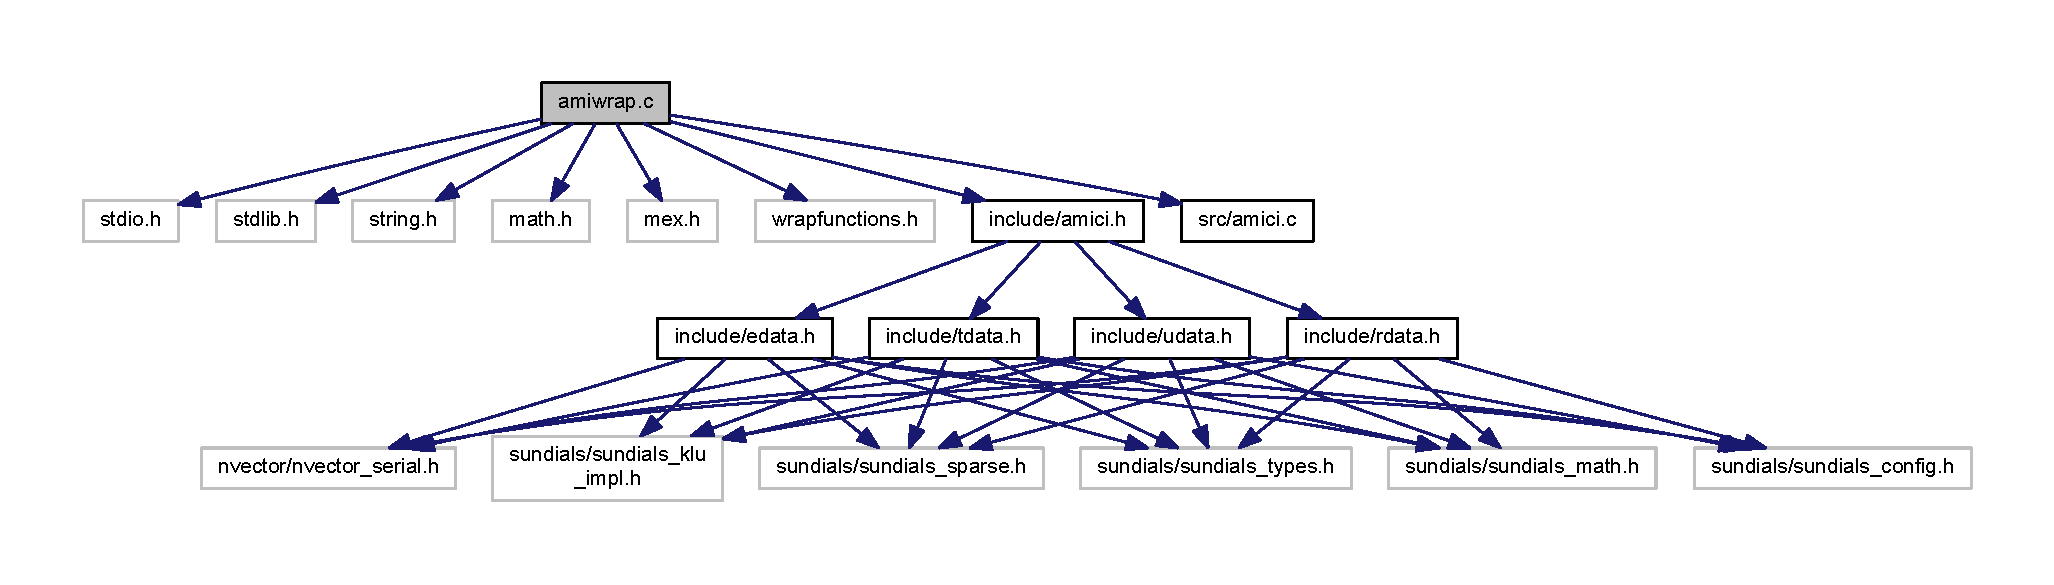
\includegraphics[width=350pt]{amiwrap_8c__incl}
\end{center}
\end{figure}
This graph shows which files directly or indirectly include this file\+:\nopagebreak
\begin{figure}[H]
\begin{center}
\leavevmode
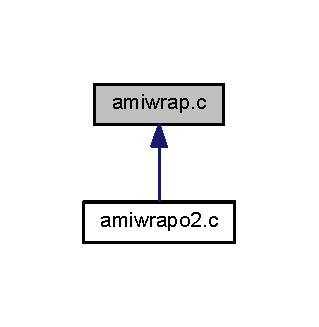
\includegraphics[width=153pt]{amiwrap_8c__dep__incl}
\end{center}
\end{figure}
\subsubsection*{Macros}
\begin{DoxyCompactItemize}
\item 
\hypertarget{amiwrap_8c_a525335710b53cb064ca56b936120431e}{}\#define {\bfseries \+\_\+\+U\+S\+E\+\_\+\+M\+A\+T\+H\+\_\+\+D\+E\+F\+I\+N\+E\+S}~/$\ast$ M\+S definition of P\+I and other constants $\ast$/\label{amiwrap_8c_a525335710b53cb064ca56b936120431e}

\item 
\hypertarget{amiwrap_8c_ae71449b1cc6e6250b91f539153a7a0d3}{}\#define {\bfseries M\+\_\+\+P\+I}~3.\+14159265358979323846\label{amiwrap_8c_ae71449b1cc6e6250b91f539153a7a0d3}

\end{DoxyCompactItemize}
\subsubsection*{Functions}
\begin{DoxyCompactItemize}
\item 
void \hyperlink{amiwrap_8c_a6a215cbfde54f82a3ce599228fc3fce5}{mex\+Function} (int nlhs, mx\+Array $\ast$plhs\mbox{[}$\,$\mbox{]}, int nrhs, const mx\+Array $\ast$prhs\mbox{[}$\,$\mbox{]})
\end{DoxyCompactItemize}


\subsubsection{Detailed Description}
This file defines the fuction mex\+Function which is executed upon calling the mex file from matlab 

\subsubsection{Function Documentation}
\hypertarget{amiwrap_8c_a6a215cbfde54f82a3ce599228fc3fce5}{}\index{amiwrap.\+c@{amiwrap.\+c}!mex\+Function@{mex\+Function}}
\index{mex\+Function@{mex\+Function}!amiwrap.\+c@{amiwrap.\+c}}
\paragraph[{mex\+Function(int nlhs, mx\+Array $\ast$plhs[], int nrhs, const mx\+Array $\ast$prhs[])}]{\setlength{\rightskip}{0pt plus 5cm}void mex\+Function (
\begin{DoxyParamCaption}
\item[{int}]{nlhs, }
\item[{mx\+Array $\ast$}]{plhs\mbox{[}$\,$\mbox{]}, }
\item[{int}]{nrhs, }
\item[{const mx\+Array $\ast$}]{prhs\mbox{[}$\,$\mbox{]}}
\end{DoxyParamCaption}
)}\label{amiwrap_8c_a6a215cbfde54f82a3ce599228fc3fce5}
mex\+Function is the main function of the mex simulation file this function carries out all numerical integration and writes results into the sol struct.


\begin{DoxyParams}[1]{Parameters}
\mbox{\tt in}  & {\em nlhs} & number of output arguments of the matlab call ~\newline
{\bfseries Type}\+: int \\
\hline
\mbox{\tt out}  & {\em plhs} & pointer to the array of output arguments ~\newline
{\bfseries Type}\+: mx\+Array \\
\hline
\mbox{\tt in}  & {\em nrhs} & number of input arguments of the matlab call ~\newline
{\bfseries Type}\+: int \\
\hline
\mbox{\tt in}  & {\em prhs} & pointer to the array of input arguments ~\newline
{\bfseries Type}\+: mx\+Array \\
\hline
\end{DoxyParams}
\begin{DoxyReturn}{Returns}
void 
\end{DoxyReturn}


Definition at line 30 of file amiwrap.\+c.



Here is the call graph for this function\+:\nopagebreak
\begin{figure}[H]
\begin{center}
\leavevmode
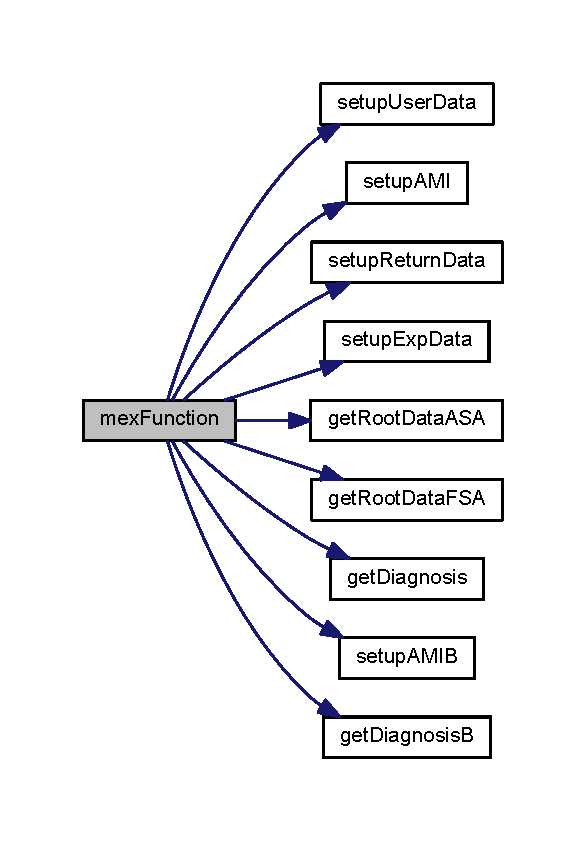
\includegraphics[width=350pt]{amiwrap_8c_a6a215cbfde54f82a3ce599228fc3fce5_cgraph}
\end{center}
\end{figure}



\hypertarget{amiwrap_8m}{}\subsection{amiwrap.\+m File Reference}
\label{amiwrap_8m}\index{amiwrap.\+m@{amiwrap.\+m}}


A\+M\+I\+W\+R\+A\+P generates c mex files for the simulation of systems of differential equations via C\+V\+O\+D\+E\+S and I\+D\+A\+S.  


\subsubsection*{Functions}
\begin{DoxyCompactItemize}
\item 
noret\+::substitute \hyperlink{amiwrap_8m_a183dd11adc4bd525147faa2590ea325b}{amiwrap} (matlabtypesubstitute varargin)
\begin{DoxyCompactList}\small\item\em A\+M\+I\+W\+R\+A\+P generates c mex files for the simulation of systems of differential equations via C\+V\+O\+D\+E\+S and I\+D\+A\+S. \end{DoxyCompactList}\end{DoxyCompactItemize}


\subsubsection{Function Documentation}
\hypertarget{amiwrap_8m_a183dd11adc4bd525147faa2590ea325b}{}\index{amiwrap.\+m@{amiwrap.\+m}!amiwrap@{amiwrap}}
\index{amiwrap@{amiwrap}!amiwrap.\+m@{amiwrap.\+m}}
\paragraph[{amiwrap(matlabtypesubstitute varargin)}]{\setlength{\rightskip}{0pt plus 5cm}noret\+::substitute amiwrap (
\begin{DoxyParamCaption}
\item[{matlabtypesubstitute}]{varargin}
\end{DoxyParamCaption}
)}\label{amiwrap_8m_a183dd11adc4bd525147faa2590ea325b}

\begin{DoxyParams}{Parameters}
{\em varargin} & 
\begin{DoxyCode}
1 amiwrap ( modelname, symfun, tdir, o2flag ) 
\end{DoxyCode}
 {\itshape Required Parameters for varargin\+:}
\begin{DoxyItemize}
\item  modelname specifies the name of the model which will be later used for the naming of the simualation file
\item  symfun specifies a function which executes model defition see \hyperlink{def_simu_definition}{Model Definition} for details
\item  tdir target directory where the simulation file should be placed {\bfseries Default\+:} \$\+A\+M\+I\+C\+I\+D\+I\+R/models/modelname
\item  o2flag boolean whether second order sensitivities should be enabled {\bfseries Default\+:} false
\end{DoxyItemize}\\
\hline
\end{DoxyParams}

\begin{DoxyRetVals}{Return values}
{\em o2flag} & void \\
\hline
\end{DoxyRetVals}


Definition at line 17 of file amiwrap.\+m.


\hypertarget{_s_b_m_l2_a_m_i_c_i_8m}{}\subsection{S\+B\+M\+L2\+A\+M\+I\+C\+I.\+m File Reference}
\label{_s_b_m_l2_a_m_i_c_i_8m}\index{S\+B\+M\+L2\+A\+M\+I\+C\+I.\+m@{S\+B\+M\+L2\+A\+M\+I\+C\+I.\+m}}


S\+B\+M\+L2\+A\+M\+I\+C\+I generates A\+M\+I\+C\+I model definition files from S\+B\+M\+L.  


\subsubsection*{Functions}
\begin{DoxyCompactItemize}
\item 
noret\+::substitute \hyperlink{_s_b_m_l2_a_m_i_c_i_8m_a11657ca9a5b1f74cf3d886a0a00f1209}{S\+B\+M\+L2\+A\+M\+I\+C\+I} (matlabtypesubstitute filename, matlabtypesubstitute modelname)
\begin{DoxyCompactList}\small\item\em S\+B\+M\+L2\+A\+M\+I\+C\+I generates A\+M\+I\+C\+I model definition files from S\+B\+M\+L. \end{DoxyCompactList}\end{DoxyCompactItemize}


\subsubsection{Function Documentation}
\hypertarget{_s_b_m_l2_a_m_i_c_i_8m_a11657ca9a5b1f74cf3d886a0a00f1209}{}\index{S\+B\+M\+L2\+A\+M\+I\+C\+I.\+m@{S\+B\+M\+L2\+A\+M\+I\+C\+I.\+m}!S\+B\+M\+L2\+A\+M\+I\+C\+I@{S\+B\+M\+L2\+A\+M\+I\+C\+I}}
\index{S\+B\+M\+L2\+A\+M\+I\+C\+I@{S\+B\+M\+L2\+A\+M\+I\+C\+I}!S\+B\+M\+L2\+A\+M\+I\+C\+I.\+m@{S\+B\+M\+L2\+A\+M\+I\+C\+I.\+m}}
\paragraph[{S\+B\+M\+L2\+A\+M\+I\+C\+I(matlabtypesubstitute filename, matlabtypesubstitute modelname)}]{\setlength{\rightskip}{0pt plus 5cm}noret\+::substitute S\+B\+M\+L2\+A\+M\+I\+C\+I (
\begin{DoxyParamCaption}
\item[{matlabtypesubstitute}]{filename, }
\item[{matlabtypesubstitute}]{modelname}
\end{DoxyParamCaption}
)}\label{_s_b_m_l2_a_m_i_c_i_8m_a11657ca9a5b1f74cf3d886a0a00f1209}

\begin{DoxyParams}{Parameters}
{\em filename} & name of the S\+B\+M\+L file (withouth extension) \\
\hline
{\em modelname} & name of the model, this will define the name of the output file\\
\hline
\end{DoxyParams}

\begin{DoxyRetVals}{Return values}
{\em modelname} & void \\
\hline
\end{DoxyRetVals}


Definition at line 17 of file S\+B\+M\+L2\+A\+M\+I\+C\+I.\+m.


\hypertarget{amici_8c}{}\subsection{src/amici.c File Reference}
\label{amici_8c}\index{src/amici.\+c@{src/amici.\+c}}


core routines for integration  


This graph shows which files directly or indirectly include this file\+:\nopagebreak
\begin{figure}[H]
\begin{center}
\leavevmode
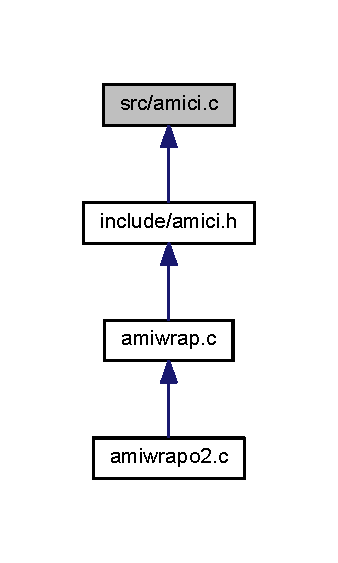
\includegraphics[width=162pt]{amici_8c__dep__incl}
\end{center}
\end{figure}
\subsubsection*{Macros}
\begin{DoxyCompactItemize}
\item 
\#define \hyperlink{amici_8c_ac6122ebe2083e778af689c6d3ba64aaf}{amici\+\_\+c}
\item 
\#define \hyperlink{amici_8c_a15c09363d6bdc7162c154ab2a20ec545}{A\+M\+I\+\_\+\+S\+U\+C\+C\+E\+S\+S}~0
\end{DoxyCompactItemize}
\subsubsection*{Functions}
\begin{DoxyCompactItemize}
\item 
\hyperlink{struct_user_data}{User\+Data} \hyperlink{amici_8c_aaa3b0319b9104865ac61df2ea87b8a13}{setup\+User\+Data} (const mx\+Array $\ast$prhs\mbox{[}$\,$\mbox{]})
\item 
void $\ast$ \hyperlink{amici_8c_a1f59a60d757981b9a2196bc6b3491027}{setup\+A\+M\+I} (int $\ast$status, void $\ast$user\+\_\+data, void $\ast$temp\+\_\+data)
\item 
void \hyperlink{amici_8c_a3899f1dc888ee4e27c36d139dd938fc0}{setup\+A\+M\+I\+B} (int $\ast$status, void $\ast$ami\+\_\+mem, void $\ast$user\+\_\+data, void $\ast$temp\+\_\+data)
\item 
\hyperlink{struct_return_data}{Return\+Data} \hyperlink{amici_8c_af60e81f8da9f9fe2ef8cdc8549a48ce1}{setup\+Return\+Data} (const mx\+Array $\ast$prhs\mbox{[}$\,$\mbox{]}, void $\ast$user\+\_\+data)
\item 
\hyperlink{struct_exp_data}{Exp\+Data} \hyperlink{amici_8c_a3c8f6481c1efc210fe8d82c618ddfcca}{setup\+Exp\+Data} (const mx\+Array $\ast$prhs\mbox{[}$\,$\mbox{]}, void $\ast$user\+\_\+data)
\item 
void \hyperlink{amici_8c_a85cdb132d0e8a2682f83f4c9603369a0}{get\+Root\+Data\+F\+S\+A} (int $\ast$status, int $\ast$nroots, void $\ast$ami\+\_\+mem, void $\ast$user\+\_\+data, void $\ast$return\+\_\+data, void $\ast$temp\+\_\+data)
\item 
void \hyperlink{amici_8c_a3c17fa40a52b536834ef24655e1bee21}{get\+Root\+Data\+A\+S\+A} (int $\ast$status, int $\ast$nroots, int $\ast$idisc, void $\ast$ami\+\_\+mem, void $\ast$user\+\_\+data, void $\ast$return\+\_\+data, void $\ast$exp\+\_\+data, void $\ast$temp\+\_\+data)
\item 
void \hyperlink{amici_8c_a13d94826e6a875f0e06ec633a88dd551}{get\+Diagnosis} (int $\ast$status, int it, void $\ast$ami\+\_\+mem, void $\ast$user\+\_\+data, void $\ast$return\+\_\+data)
\item 
void \hyperlink{amici_8c_a90da28fbc4745516101db3c8d6be9305}{get\+Diagnosis\+B} (int $\ast$status, int it, void $\ast$ami\+\_\+mem, void $\ast$user\+\_\+data, void $\ast$return\+\_\+data, void $\ast$temp\+\_\+data)
\end{DoxyCompactItemize}


\subsubsection{Macro Definition Documentation}
\hypertarget{amici_8c_ac6122ebe2083e778af689c6d3ba64aaf}{}\index{amici.\+c@{amici.\+c}!amici\+\_\+c@{amici\+\_\+c}}
\index{amici\+\_\+c@{amici\+\_\+c}!amici.\+c@{amici.\+c}}
\paragraph[{amici\+\_\+c}]{\setlength{\rightskip}{0pt plus 5cm}\#define amici\+\_\+c}\label{amici_8c_ac6122ebe2083e778af689c6d3ba64aaf}
include guard 

Definition at line 8 of file amici.\+c.

\hypertarget{amici_8c_a15c09363d6bdc7162c154ab2a20ec545}{}\index{amici.\+c@{amici.\+c}!A\+M\+I\+\_\+\+S\+U\+C\+C\+E\+S\+S@{A\+M\+I\+\_\+\+S\+U\+C\+C\+E\+S\+S}}
\index{A\+M\+I\+\_\+\+S\+U\+C\+C\+E\+S\+S@{A\+M\+I\+\_\+\+S\+U\+C\+C\+E\+S\+S}!amici.\+c@{amici.\+c}}
\paragraph[{A\+M\+I\+\_\+\+S\+U\+C\+C\+E\+S\+S}]{\setlength{\rightskip}{0pt plus 5cm}\#define A\+M\+I\+\_\+\+S\+U\+C\+C\+E\+S\+S~0}\label{amici_8c_a15c09363d6bdc7162c154ab2a20ec545}
return value indicating successful execution 

Definition at line 10 of file amici.\+c.



\subsubsection{Function Documentation}
\hypertarget{amici_8c_aaa3b0319b9104865ac61df2ea87b8a13}{}\index{amici.\+c@{amici.\+c}!setup\+User\+Data@{setup\+User\+Data}}
\index{setup\+User\+Data@{setup\+User\+Data}!amici.\+c@{amici.\+c}}
\paragraph[{setup\+User\+Data(const mx\+Array $\ast$prhs[])}]{\setlength{\rightskip}{0pt plus 5cm}{\bf User\+Data} setup\+User\+Data (
\begin{DoxyParamCaption}
\item[{const mx\+Array $\ast$}]{prhs\mbox{[}$\,$\mbox{]}}
\end{DoxyParamCaption}
)}\label{amici_8c_aaa3b0319b9104865ac61df2ea87b8a13}
setup\+User\+Data extracts information from the matlab call and returns the corresponding \hyperlink{struct_user_data}{User\+Data} struct 
\begin{DoxyParams}[1]{Parameters}
\mbox{\tt in}  & {\em prhs} & pointer to the array of input arguments ~\newline
{\bfseries Type}\+: mx\+Array \\
\hline
\end{DoxyParams}
\begin{DoxyReturn}{Returns}
udata\+: struct containing all provided user data
\end{DoxyReturn}


Definition at line 12 of file amici.\+c.



Here is the caller graph for this function\+:\nopagebreak
\begin{figure}[H]
\begin{center}
\leavevmode
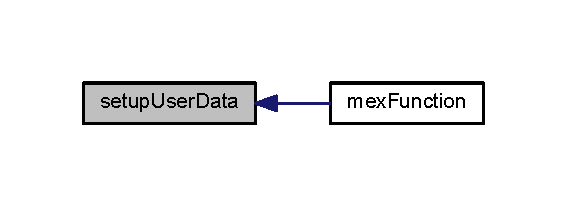
\includegraphics[width=272pt]{amici_8c_aaa3b0319b9104865ac61df2ea87b8a13_icgraph}
\end{center}
\end{figure}


\hypertarget{amici_8c_a1f59a60d757981b9a2196bc6b3491027}{}\index{amici.\+c@{amici.\+c}!setup\+A\+M\+I@{setup\+A\+M\+I}}
\index{setup\+A\+M\+I@{setup\+A\+M\+I}!amici.\+c@{amici.\+c}}
\paragraph[{setup\+A\+M\+I(int $\ast$status, void $\ast$user\+\_\+data, void $\ast$temp\+\_\+data)}]{\setlength{\rightskip}{0pt plus 5cm}void$\ast$ setup\+A\+M\+I (
\begin{DoxyParamCaption}
\item[{int $\ast$}]{status, }
\item[{void $\ast$}]{user\+\_\+data, }
\item[{void $\ast$}]{temp\+\_\+data}
\end{DoxyParamCaption}
)}\label{amici_8c_a1f59a60d757981b9a2196bc6b3491027}
setup\+A\+M\+Is initialises the ami memory object 
\begin{DoxyParams}[1]{Parameters}
\mbox{\tt out}  & {\em status} & flag indicating success of execution ~\newline
{\bfseries Type}\+: $\ast$int \\
\hline
\mbox{\tt in}  & {\em user\+\_\+data} & pointer to the user data struct ~\newline
{\bfseries Type}\+: \hyperlink{struct_user_data}{User\+Data} \\
\hline
\mbox{\tt in}  & {\em temp\+\_\+data} & pointer to the temporary data struct ~\newline
{\bfseries Type}\+: \hyperlink{struct_temp_data}{Temp\+Data} \\
\hline
\end{DoxyParams}
\begin{DoxyReturn}{Returns}
void
\end{DoxyReturn}


Definition at line 151 of file amici.\+c.



Here is the caller graph for this function\+:\nopagebreak
\begin{figure}[H]
\begin{center}
\leavevmode
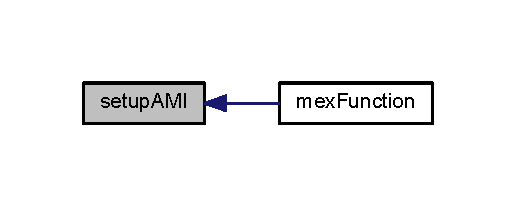
\includegraphics[width=247pt]{amici_8c_a1f59a60d757981b9a2196bc6b3491027_icgraph}
\end{center}
\end{figure}


\hypertarget{amici_8c_a3899f1dc888ee4e27c36d139dd938fc0}{}\index{amici.\+c@{amici.\+c}!setup\+A\+M\+I\+B@{setup\+A\+M\+I\+B}}
\index{setup\+A\+M\+I\+B@{setup\+A\+M\+I\+B}!amici.\+c@{amici.\+c}}
\paragraph[{setup\+A\+M\+I\+B(int $\ast$status, void $\ast$ami\+\_\+mem, void $\ast$user\+\_\+data, void $\ast$temp\+\_\+data)}]{\setlength{\rightskip}{0pt plus 5cm}void setup\+A\+M\+I\+B (
\begin{DoxyParamCaption}
\item[{int $\ast$}]{status, }
\item[{void $\ast$}]{ami\+\_\+mem, }
\item[{void $\ast$}]{user\+\_\+data, }
\item[{void $\ast$}]{temp\+\_\+data}
\end{DoxyParamCaption}
)}\label{amici_8c_a3899f1dc888ee4e27c36d139dd938fc0}
setup\+A\+M\+I\+B initialises the A\+M\+I memory object for the backwards problem 
\begin{DoxyParams}[1]{Parameters}
\mbox{\tt out}  & {\em status} & flag indicating success of execution ~\newline
{\bfseries Type}\+: $\ast$int \\
\hline
\mbox{\tt in}  & {\em ami\+\_\+mem} & pointer to the solver memory object of the forward problem \\
\hline
\mbox{\tt in}  & {\em user\+\_\+data} & pointer to the user data struct ~\newline
{\bfseries Type}\+: \hyperlink{struct_user_data}{User\+Data} \\
\hline
\mbox{\tt in}  & {\em temp\+\_\+data} & pointer to the temporary data struct ~\newline
{\bfseries Type}\+: \hyperlink{struct_temp_data}{Temp\+Data} \\
\hline
\end{DoxyParams}
\begin{DoxyReturn}{Returns}
void
\end{DoxyReturn}


Definition at line 436 of file amici.\+c.



Here is the caller graph for this function\+:\nopagebreak
\begin{figure}[H]
\begin{center}
\leavevmode
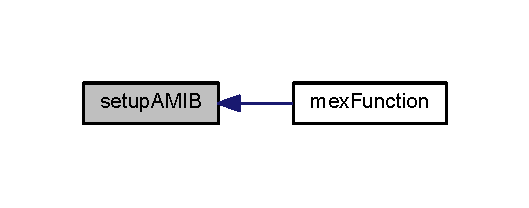
\includegraphics[width=254pt]{amici_8c_a3899f1dc888ee4e27c36d139dd938fc0_icgraph}
\end{center}
\end{figure}


\hypertarget{amici_8c_af60e81f8da9f9fe2ef8cdc8549a48ce1}{}\index{amici.\+c@{amici.\+c}!setup\+Return\+Data@{setup\+Return\+Data}}
\index{setup\+Return\+Data@{setup\+Return\+Data}!amici.\+c@{amici.\+c}}
\paragraph[{setup\+Return\+Data(const mx\+Array $\ast$prhs[], void $\ast$user\+\_\+data)}]{\setlength{\rightskip}{0pt plus 5cm}{\bf Return\+Data} setup\+Return\+Data (
\begin{DoxyParamCaption}
\item[{const mx\+Array $\ast$}]{prhs\mbox{[}$\,$\mbox{]}, }
\item[{void $\ast$}]{user\+\_\+data}
\end{DoxyParamCaption}
)}\label{amici_8c_af60e81f8da9f9fe2ef8cdc8549a48ce1}
setup\+Return\+Data initialises the return data struct 
\begin{DoxyParams}[1]{Parameters}
\mbox{\tt in}  & {\em prhs} & user input ~\newline
{\bfseries Type}\+: $\ast$mx\+Array \\
\hline
\mbox{\tt in}  & {\em user\+\_\+data} & pointer to the user data struct ~\newline
{\bfseries Type}\+: \hyperlink{struct_user_data}{User\+Data} \\
\hline
\end{DoxyParams}
\begin{DoxyReturn}{Returns}
rdata\+: return data struct ~\newline
{\bfseries Type}\+: \hyperlink{struct_return_data}{Return\+Data}
\end{DoxyReturn}
user udata 

Definition at line 627 of file amici.\+c.



Here is the caller graph for this function\+:\nopagebreak
\begin{figure}[H]
\begin{center}
\leavevmode
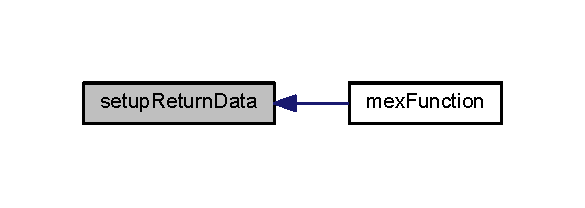
\includegraphics[width=281pt]{amici_8c_af60e81f8da9f9fe2ef8cdc8549a48ce1_icgraph}
\end{center}
\end{figure}


\hypertarget{amici_8c_a3c8f6481c1efc210fe8d82c618ddfcca}{}\index{amici.\+c@{amici.\+c}!setup\+Exp\+Data@{setup\+Exp\+Data}}
\index{setup\+Exp\+Data@{setup\+Exp\+Data}!amici.\+c@{amici.\+c}}
\paragraph[{setup\+Exp\+Data(const mx\+Array $\ast$prhs[], void $\ast$user\+\_\+data)}]{\setlength{\rightskip}{0pt plus 5cm}{\bf Exp\+Data} setup\+Exp\+Data (
\begin{DoxyParamCaption}
\item[{const mx\+Array $\ast$}]{prhs\mbox{[}$\,$\mbox{]}, }
\item[{void $\ast$}]{user\+\_\+data}
\end{DoxyParamCaption}
)}\label{amici_8c_a3c8f6481c1efc210fe8d82c618ddfcca}
setup\+Exp\+Data initialises the experimental data struct 
\begin{DoxyParams}[1]{Parameters}
\mbox{\tt in}  & {\em prhs} & user input ~\newline
{\bfseries Type}\+: $\ast$mx\+Array \\
\hline
\mbox{\tt in}  & {\em user\+\_\+data} & pointer to the user data struct ~\newline
{\bfseries Type}\+: \hyperlink{struct_user_data}{User\+Data} \\
\hline
\end{DoxyParams}
\begin{DoxyReturn}{Returns}
edata\+: experimental data struct ~\newline
{\bfseries Type}\+: \hyperlink{struct_exp_data}{Exp\+Data}
\end{DoxyReturn}
user udata 

Definition at line 692 of file amici.\+c.



Here is the caller graph for this function\+:\nopagebreak
\begin{figure}[H]
\begin{center}
\leavevmode
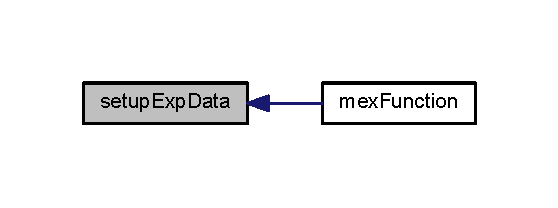
\includegraphics[width=268pt]{amici_8c_a3c8f6481c1efc210fe8d82c618ddfcca_icgraph}
\end{center}
\end{figure}


\hypertarget{amici_8c_a85cdb132d0e8a2682f83f4c9603369a0}{}\index{amici.\+c@{amici.\+c}!get\+Root\+Data\+F\+S\+A@{get\+Root\+Data\+F\+S\+A}}
\index{get\+Root\+Data\+F\+S\+A@{get\+Root\+Data\+F\+S\+A}!amici.\+c@{amici.\+c}}
\paragraph[{get\+Root\+Data\+F\+S\+A(int $\ast$status, int $\ast$nroots, void $\ast$ami\+\_\+mem, void $\ast$user\+\_\+data, void $\ast$return\+\_\+data, void $\ast$temp\+\_\+data)}]{\setlength{\rightskip}{0pt plus 5cm}void get\+Root\+Data\+F\+S\+A (
\begin{DoxyParamCaption}
\item[{int $\ast$}]{status, }
\item[{int $\ast$}]{nroots, }
\item[{void $\ast$}]{ami\+\_\+mem, }
\item[{void $\ast$}]{user\+\_\+data, }
\item[{void $\ast$}]{return\+\_\+data, }
\item[{void $\ast$}]{temp\+\_\+data}
\end{DoxyParamCaption}
)}\label{amici_8c_a85cdb132d0e8a2682f83f4c9603369a0}
get\+Root\+Data\+F\+S\+A extracts root information for forward sensitivity analysis


\begin{DoxyParams}[1]{Parameters}
\mbox{\tt out}  & {\em status} & flag indicating success of execution ~\newline
{\bfseries Type}\+: int \\
\hline
\mbox{\tt out}  & {\em nroots} & counter for the number of found roots ~\newline
{\bfseries Type}\+: int \\
\hline
\mbox{\tt in}  & {\em ami\+\_\+mem} & pointer to the solver memory block ~\newline
{\bfseries Type}\+: void \\
\hline
\mbox{\tt in}  & {\em user\+\_\+data} & pointer to the user data struct ~\newline
{\bfseries Type}\+: \hyperlink{struct_user_data}{User\+Data} \\
\hline
\mbox{\tt out}  & {\em return\+\_\+data} & pointer to the return data struct ~\newline
{\bfseries Type}\+: \hyperlink{struct_return_data}{Return\+Data} \\
\hline
\mbox{\tt out}  & {\em temp\+\_\+data} & pointer to the temporary data struct ~\newline
{\bfseries Type}\+: \hyperlink{struct_temp_data}{Temp\+Data} \\
\hline
\end{DoxyParams}
\begin{DoxyReturn}{Returns}
void
\end{DoxyReturn}


Definition at line 791 of file amici.\+c.



Here is the caller graph for this function\+:\nopagebreak
\begin{figure}[H]
\begin{center}
\leavevmode
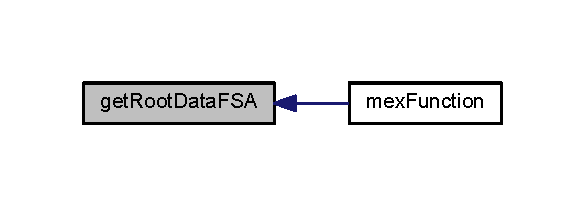
\includegraphics[width=281pt]{amici_8c_a85cdb132d0e8a2682f83f4c9603369a0_icgraph}
\end{center}
\end{figure}


\hypertarget{amici_8c_a3c17fa40a52b536834ef24655e1bee21}{}\index{amici.\+c@{amici.\+c}!get\+Root\+Data\+A\+S\+A@{get\+Root\+Data\+A\+S\+A}}
\index{get\+Root\+Data\+A\+S\+A@{get\+Root\+Data\+A\+S\+A}!amici.\+c@{amici.\+c}}
\paragraph[{get\+Root\+Data\+A\+S\+A(int $\ast$status, int $\ast$nroots, int $\ast$idisc, void $\ast$ami\+\_\+mem, void $\ast$user\+\_\+data, void $\ast$return\+\_\+data, void $\ast$exp\+\_\+data, void $\ast$temp\+\_\+data)}]{\setlength{\rightskip}{0pt plus 5cm}void get\+Root\+Data\+A\+S\+A (
\begin{DoxyParamCaption}
\item[{int $\ast$}]{status, }
\item[{int $\ast$}]{nroots, }
\item[{int $\ast$}]{idisc, }
\item[{void $\ast$}]{ami\+\_\+mem, }
\item[{void $\ast$}]{user\+\_\+data, }
\item[{void $\ast$}]{return\+\_\+data, }
\item[{void $\ast$}]{exp\+\_\+data, }
\item[{void $\ast$}]{temp\+\_\+data}
\end{DoxyParamCaption}
)}\label{amici_8c_a3c17fa40a52b536834ef24655e1bee21}
get\+Root\+Data\+A\+S\+A extracts root information for adjoint sensitivity analysis


\begin{DoxyParams}[1]{Parameters}
\mbox{\tt out}  & {\em status} & flag indicating success of execution ~\newline
{\bfseries Type}\+: $\ast$int \\
\hline
\mbox{\tt out}  & {\em nroots} & counter for the number of found roots ~\newline
{\bfseries Type}\+: $\ast$int \\
\hline
\mbox{\tt out}  & {\em idisc} & counter for the number of found discontinuities ~\newline
{\bfseries Type}\+: $\ast$int \\
\hline
\mbox{\tt in}  & {\em ami\+\_\+mem} & pointer to the solver memory block ~\newline
{\bfseries Type}\+: $\ast$void \\
\hline
\mbox{\tt in}  & {\em user\+\_\+data} & pointer to the user data struct ~\newline
{\bfseries Type}\+: \hyperlink{struct_user_data}{User\+Data} \\
\hline
\mbox{\tt out}  & {\em return\+\_\+data} & pointer to the return data struct ~\newline
{\bfseries Type}\+: \hyperlink{struct_return_data}{Return\+Data} \\
\hline
\mbox{\tt in}  & {\em exp\+\_\+data} & pointer to the experimental data struct ~\newline
{\bfseries Type}\+: \hyperlink{struct_exp_data}{Exp\+Data} \\
\hline
\mbox{\tt out}  & {\em temp\+\_\+data} & pointer to the temporary data struct ~\newline
{\bfseries Type}\+: \hyperlink{struct_temp_data}{Temp\+Data} \\
\hline
\end{DoxyParams}
\begin{DoxyReturn}{Returns}
void
\end{DoxyReturn}


Definition at line 875 of file amici.\+c.



Here is the caller graph for this function\+:\nopagebreak
\begin{figure}[H]
\begin{center}
\leavevmode
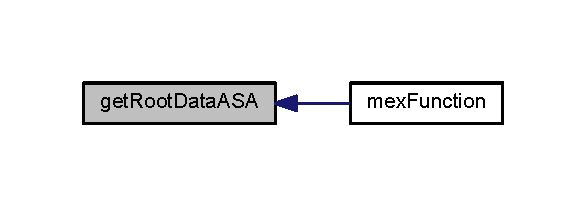
\includegraphics[width=281pt]{amici_8c_a3c17fa40a52b536834ef24655e1bee21_icgraph}
\end{center}
\end{figure}


\hypertarget{amici_8c_a13d94826e6a875f0e06ec633a88dd551}{}\index{amici.\+c@{amici.\+c}!get\+Diagnosis@{get\+Diagnosis}}
\index{get\+Diagnosis@{get\+Diagnosis}!amici.\+c@{amici.\+c}}
\paragraph[{get\+Diagnosis(int $\ast$status, int it, void $\ast$ami\+\_\+mem, void $\ast$user\+\_\+data, void $\ast$return\+\_\+data)}]{\setlength{\rightskip}{0pt plus 5cm}void get\+Diagnosis (
\begin{DoxyParamCaption}
\item[{int $\ast$}]{status, }
\item[{int}]{it, }
\item[{void $\ast$}]{ami\+\_\+mem, }
\item[{void $\ast$}]{user\+\_\+data, }
\item[{void $\ast$}]{return\+\_\+data}
\end{DoxyParamCaption}
)}\label{amici_8c_a13d94826e6a875f0e06ec633a88dd551}
get\+Diagnosis extracts diagnosis information from solver memory block and writes them into the return data struct


\begin{DoxyParams}[1]{Parameters}
\mbox{\tt out}  & {\em status} & flag indicating success of execution ~\newline
{\bfseries Type}\+: $\ast$int \\
\hline
\mbox{\tt in}  & {\em it} & time-\/point index ~\newline
{\bfseries Type}\+: int \\
\hline
\mbox{\tt in}  & {\em ami\+\_\+mem} & pointer to the solver memory block ~\newline
{\bfseries Type}\+: $\ast$void \\
\hline
\mbox{\tt in}  & {\em user\+\_\+data} & pointer to the user data struct ~\newline
{\bfseries Type}\+: \hyperlink{struct_user_data}{User\+Data} \\
\hline
\mbox{\tt out}  & {\em return\+\_\+data} & pointer to the return data struct ~\newline
{\bfseries Type}\+: \hyperlink{struct_return_data}{Return\+Data} \\
\hline
\end{DoxyParams}
\begin{DoxyReturn}{Returns}
void
\end{DoxyReturn}


Definition at line 983 of file amici.\+c.



Here is the caller graph for this function\+:\nopagebreak
\begin{figure}[H]
\begin{center}
\leavevmode
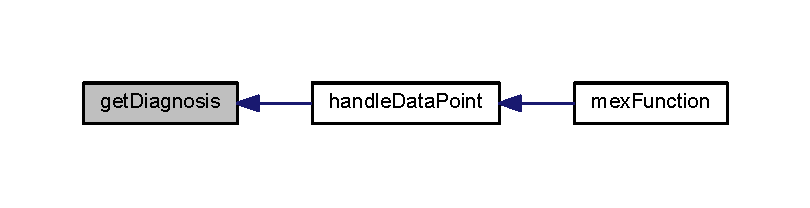
\includegraphics[width=263pt]{amici_8c_a13d94826e6a875f0e06ec633a88dd551_icgraph}
\end{center}
\end{figure}


\hypertarget{amici_8c_a90da28fbc4745516101db3c8d6be9305}{}\index{amici.\+c@{amici.\+c}!get\+Diagnosis\+B@{get\+Diagnosis\+B}}
\index{get\+Diagnosis\+B@{get\+Diagnosis\+B}!amici.\+c@{amici.\+c}}
\paragraph[{get\+Diagnosis\+B(int $\ast$status, int it, void $\ast$ami\+\_\+mem, void $\ast$user\+\_\+data, void $\ast$return\+\_\+data, void $\ast$temp\+\_\+data)}]{\setlength{\rightskip}{0pt plus 5cm}void get\+Diagnosis\+B (
\begin{DoxyParamCaption}
\item[{int $\ast$}]{status, }
\item[{int}]{it, }
\item[{void $\ast$}]{ami\+\_\+mem, }
\item[{void $\ast$}]{user\+\_\+data, }
\item[{void $\ast$}]{return\+\_\+data, }
\item[{void $\ast$}]{temp\+\_\+data}
\end{DoxyParamCaption}
)}\label{amici_8c_a90da28fbc4745516101db3c8d6be9305}
get\+Diagnosis extracts diagnosis information from solver memory block and writes them into the return data struct


\begin{DoxyParams}[1]{Parameters}
\mbox{\tt out}  & {\em status} & flag indicating success of execution ~\newline
{\bfseries Type}\+: $\ast$int \\
\hline
\mbox{\tt in}  & {\em it} & time-\/point index ~\newline
{\bfseries Type}\+: int \\
\hline
\mbox{\tt in}  & {\em ami\+\_\+mem} & pointer to the solver memory block ~\newline
{\bfseries Type}\+: $\ast$void \\
\hline
\mbox{\tt in}  & {\em user\+\_\+data} & pointer to the user data struct ~\newline
{\bfseries Type}\+: \hyperlink{struct_user_data}{User\+Data} \\
\hline
\mbox{\tt out}  & {\em return\+\_\+data} & pointer to the return data struct ~\newline
{\bfseries Type}\+: \hyperlink{struct_return_data}{Return\+Data} \\
\hline
\mbox{\tt out}  & {\em temp\+\_\+data} & pointer to the temporary data struct ~\newline
{\bfseries Type}\+: \hyperlink{struct_temp_data}{Temp\+Data} \\
\hline
\end{DoxyParams}
\begin{DoxyReturn}{Returns}
void
\end{DoxyReturn}


Definition at line 1017 of file amici.\+c.



Here is the caller graph for this function\+:\nopagebreak
\begin{figure}[H]
\begin{center}
\leavevmode
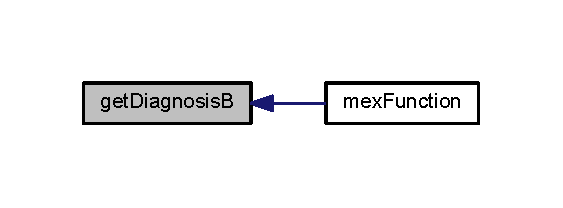
\includegraphics[width=270pt]{amici_8c_a90da28fbc4745516101db3c8d6be9305_icgraph}
\end{center}
\end{figure}



\hypertarget{spline_8c}{}\subsection{src/spline.c File Reference}
\label{spline_8c}\index{src/spline.\+c@{src/spline.\+c}}


definition of spline functions  


This graph shows which files directly or indirectly include this file\+:\nopagebreak
\begin{figure}[H]
\begin{center}
\leavevmode
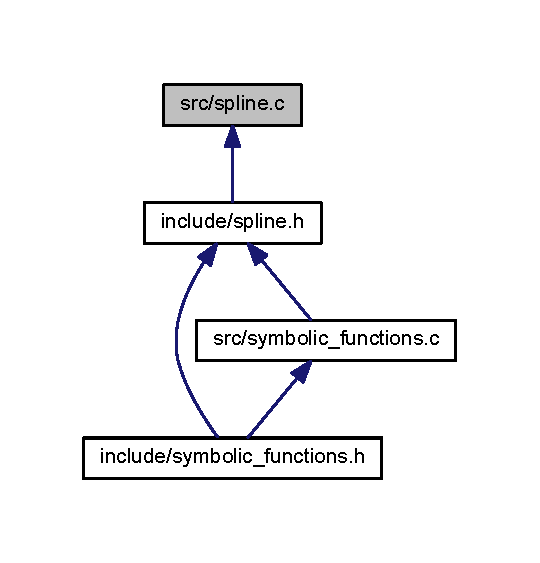
\includegraphics[width=204pt]{spline_8c__dep__incl}
\end{center}
\end{figure}
\subsubsection*{Functions}
\begin{DoxyCompactItemize}
\item 
int \hyperlink{spline_8c_aa6801bbdb0c7625719c019ac287be29e}{spline} (int n, int end1, int end2, double slope1, double slope2, double x\mbox{[}$\,$\mbox{]}, double y\mbox{[}$\,$\mbox{]}, double b\mbox{[}$\,$\mbox{]}, double c\mbox{[}$\,$\mbox{]}, double d\mbox{[}$\,$\mbox{]})
\item 
double \hyperlink{spline_8c_a20c8c27889853621fba3e0eacd333723}{seval} (int n, double u, double x\mbox{[}$\,$\mbox{]}, double y\mbox{[}$\,$\mbox{]}, double b\mbox{[}$\,$\mbox{]}, double c\mbox{[}$\,$\mbox{]}, double d\mbox{[}$\,$\mbox{]})
\item 
double \hyperlink{spline_8c_a7fc66f543b0c296fa694a90c03edb6ca}{deriv} (int n, double u, double x\mbox{[}$\,$\mbox{]}, double b\mbox{[}$\,$\mbox{]}, double c\mbox{[}$\,$\mbox{]}, double d\mbox{[}$\,$\mbox{]})
\item 
double \hyperlink{spline_8c_a158da90aec69a4796fb6f350ac6b71ab}{sinteg} (int n, double u, double x\mbox{[}$\,$\mbox{]}, double y\mbox{[}$\,$\mbox{]}, double b\mbox{[}$\,$\mbox{]}, double c\mbox{[}$\,$\mbox{]}, double d\mbox{[}$\,$\mbox{]})
\end{DoxyCompactItemize}


\subsubsection{Detailed Description}
\begin{DoxyAuthor}{Author}
Peter \& Nigel, Design Software, 42 Gubberley St, Kenmore, 4069, Australia. 
\end{DoxyAuthor}


\subsubsection{Function Documentation}
\hypertarget{spline_8c_aa6801bbdb0c7625719c019ac287be29e}{}\index{spline.\+c@{spline.\+c}!spline@{spline}}
\index{spline@{spline}!spline.\+c@{spline.\+c}}
\paragraph[{spline(int n, int end1, int end2, double slope1, double slope2, double x[], double y[], double b[], double c[], double d[])}]{\setlength{\rightskip}{0pt plus 5cm}int spline (
\begin{DoxyParamCaption}
\item[{int}]{n, }
\item[{int}]{end1, }
\item[{int}]{end2, }
\item[{double}]{slope1, }
\item[{double}]{slope2, }
\item[{double}]{x\mbox{[}$\,$\mbox{]}, }
\item[{double}]{y\mbox{[}$\,$\mbox{]}, }
\item[{double}]{b\mbox{[}$\,$\mbox{]}, }
\item[{double}]{c\mbox{[}$\,$\mbox{]}, }
\item[{double}]{d\mbox{[}$\,$\mbox{]}}
\end{DoxyParamCaption}
)}\label{spline_8c_aa6801bbdb0c7625719c019ac287be29e}
Evaluate the coefficients b\mbox{[}i\mbox{]}, c\mbox{[}i\mbox{]}, d\mbox{[}i\mbox{]}, i = 0, 1, .. n-\/1 for a cubic interpolating spline

S(xx) = Y\mbox{[}i\mbox{]} + b\mbox{[}i\mbox{]} $\ast$ w + c\mbox{[}i\mbox{]} $\ast$ w$\ast$$\ast$2 + d\mbox{[}i\mbox{]} $\ast$ w$\ast$$\ast$3 where w = xx -\/ x\mbox{[}i\mbox{]} and x\mbox{[}i\mbox{]} $<$= xx $<$= x\mbox{[}i+1\mbox{]}

The n supplied data points are x\mbox{[}i\mbox{]}, y\mbox{[}i\mbox{]}, i = 0 ... n-\/1.


\begin{DoxyParams}[1]{Parameters}
\mbox{\tt in}  & {\em n} & The number of data points or knots (n $>$= 2) \\
\hline
\mbox{\tt in}  & {\em end1} & 0\+: default condition 1\+: specify the slopes at x\mbox{[}0\mbox{]} \\
\hline
\mbox{\tt in}  & {\em end2} & 0\+: default condition 1\+: specify the slopes at x\mbox{[}n-\/1\mbox{]} \\
\hline
\mbox{\tt in}  & {\em slope1} & slope at x\mbox{[}0\mbox{]} \\
\hline
\mbox{\tt in}  & {\em slope2} & slope at x\mbox{[}n-\/1\mbox{]} \\
\hline
\mbox{\tt in}  & {\em x\mbox{[}$\,$\mbox{]}} & the abscissas of the knots in strictly increasing order \\
\hline
\mbox{\tt in}  & {\em y\mbox{[}$\,$\mbox{]}} & the ordinates of the knots \\
\hline
\mbox{\tt out}  & {\em b\mbox{[}$\,$\mbox{]}} & array of spline coefficients \\
\hline
\mbox{\tt out}  & {\em c\mbox{[}$\,$\mbox{]}} & array of spline coefficients \\
\hline
\mbox{\tt out}  & {\em d\mbox{[}$\,$\mbox{]}} & array of spline coefficients\\
\hline
\end{DoxyParams}

\begin{DoxyRetVals}{Return values}
{\em 0} & normal return \\
\hline
{\em 1} & less than two data points; cannot interpolate \\
\hline
{\em 2} & x\mbox{[}\mbox{]} are not in ascending order\\
\hline
\end{DoxyRetVals}
\paragraph*{Notes }


\begin{DoxyItemize}
\item The accompanying function \hyperlink{spline_8c_a20c8c27889853621fba3e0eacd333723}{seval()} may be used to evaluate the spline while deriv will provide the first derivative.
\item Using p to denote differentiation y\mbox{[}i\mbox{]} = S(\+X\mbox{[}i\mbox{]}) b\mbox{[}i\mbox{]} = Sp(\+X\mbox{[}i\mbox{]}) c\mbox{[}i\mbox{]} = Spp(\+X\mbox{[}i\mbox{]})/2 d\mbox{[}i\mbox{]} = Sppp(\+X\mbox{[}i\mbox{]})/6 ( Derivative from the right )
\item Since the zero elements of the arrays A\+R\+E N\+O\+W used here, all arrays to be passed from the main program should be dimensioned at least \mbox{[}n\mbox{]}. These routines will use elements \mbox{[}0 .. n-\/1\mbox{]}.
\item Adapted from the text Forsythe, G.\+E., Malcolm, M.\+A. and Moler, C.\+B. (1977) \char`\"{}\+Computer Methods for Mathematical Computations\char`\"{} Prentice Hall
\item Note that although there are only n-\/1 polynomial segments, n elements are requird in b, c, d. The elements b\mbox{[}n-\/1\mbox{]}, c\mbox{[}n-\/1\mbox{]} and d\mbox{[}n-\/1\mbox{]} are set to continue the last segment past x\mbox{[}n-\/1\mbox{]}. 
\end{DoxyItemize}

Definition at line 66 of file spline.\+c.

\hypertarget{spline_8c_a20c8c27889853621fba3e0eacd333723}{}\index{spline.\+c@{spline.\+c}!seval@{seval}}
\index{seval@{seval}!spline.\+c@{spline.\+c}}
\paragraph[{seval(int n, double u, double x[], double y[], double b[], double c[], double d[])}]{\setlength{\rightskip}{0pt plus 5cm}double seval (
\begin{DoxyParamCaption}
\item[{int}]{n, }
\item[{double}]{u, }
\item[{double}]{x\mbox{[}$\,$\mbox{]}, }
\item[{double}]{y\mbox{[}$\,$\mbox{]}, }
\item[{double}]{b\mbox{[}$\,$\mbox{]}, }
\item[{double}]{c\mbox{[}$\,$\mbox{]}, }
\item[{double}]{d\mbox{[}$\,$\mbox{]}}
\end{DoxyParamCaption}
)}\label{spline_8c_a20c8c27889853621fba3e0eacd333723}
Evaluate the cubic spline function

S(xx) = y\mbox{[}i\mbox{]} + b\mbox{[}i\mbox{]} $\ast$ w + c\mbox{[}i\mbox{]} $\ast$ w$\ast$$\ast$2 + d\mbox{[}i\mbox{]} $\ast$ w$\ast$$\ast$3 where w = u -\/ x\mbox{[}i\mbox{]} and x\mbox{[}i\mbox{]} $<$= u $<$= x\mbox{[}i+1\mbox{]} Note that Horner\textquotesingle{}s rule is used. If u $<$ x\mbox{[}0\mbox{]} then i = 0 is used. If u $>$ x\mbox{[}n-\/1\mbox{]} then i = n-\/1 is used.


\begin{DoxyParams}[1]{Parameters}
\mbox{\tt in}  & {\em n} & The number of data points or knots (n $>$= 2) \\
\hline
\mbox{\tt in}  & {\em u} & the abscissa at which the spline is to be evaluated \\
\hline
\mbox{\tt in}  & {\em x\mbox{[}$\,$\mbox{]}} & the abscissas of the knots in strictly increasing order \\
\hline
\mbox{\tt in}  & {\em y\mbox{[}$\,$\mbox{]}} & the ordinates of the knots \\
\hline
\mbox{\tt in}  & {\em b} & array of spline coefficients computed by \hyperlink{spline_8c_aa6801bbdb0c7625719c019ac287be29e}{spline()}. \\
\hline
\mbox{\tt in}  & {\em c} & array of spline coefficients computed by \hyperlink{spline_8c_aa6801bbdb0c7625719c019ac287be29e}{spline()}. \\
\hline
\mbox{\tt in}  & {\em d} & array of spline coefficients computed by \hyperlink{spline_8c_aa6801bbdb0c7625719c019ac287be29e}{spline()}.\\
\hline
\end{DoxyParams}
\begin{DoxyReturn}{Returns}
the value of the spline function at u
\end{DoxyReturn}
Notes
\begin{DoxyItemize}
\item If u is not in the same interval as the previous call then a binary search is performed to determine the proper interval. 
\end{DoxyItemize}

Definition at line 208 of file spline.\+c.

\hypertarget{spline_8c_a7fc66f543b0c296fa694a90c03edb6ca}{}\index{spline.\+c@{spline.\+c}!deriv@{deriv}}
\index{deriv@{deriv}!spline.\+c@{spline.\+c}}
\paragraph[{deriv(int n, double u, double x[], double b[], double c[], double d[])}]{\setlength{\rightskip}{0pt plus 5cm}double deriv (
\begin{DoxyParamCaption}
\item[{int}]{n, }
\item[{double}]{u, }
\item[{double}]{x\mbox{[}$\,$\mbox{]}, }
\item[{double}]{b\mbox{[}$\,$\mbox{]}, }
\item[{double}]{c\mbox{[}$\,$\mbox{]}, }
\item[{double}]{d\mbox{[}$\,$\mbox{]}}
\end{DoxyParamCaption}
)}\label{spline_8c_a7fc66f543b0c296fa694a90c03edb6ca}
Evaluate the derivative of the cubic spline function

S(x) = B\mbox{[}i\mbox{]} + 2.\+0 $\ast$ C\mbox{[}i\mbox{]} $\ast$ w + 3.\+0 $\ast$ D\mbox{[}i\mbox{]} $\ast$ w$\ast$$\ast$2 where w = u -\/ X\mbox{[}i\mbox{]} and X\mbox{[}i\mbox{]} $<$= u $<$= X\mbox{[}i+1\mbox{]} Note that Horner\textquotesingle{}s rule is used. If U $<$ X\mbox{[}0\mbox{]} then i = 0 is used. If U $>$ X\mbox{[}n-\/1\mbox{]} then i = n-\/1 is used.


\begin{DoxyParams}[1]{Parameters}
\mbox{\tt in}  & {\em n} & the number of data points or knots (n $>$= 2) \\
\hline
\mbox{\tt in}  & {\em u} & the abscissa at which the derivative is to be evaluated \\
\hline
\mbox{\tt in}  & {\em x} & the abscissas of the knots in strictly increasing order \\
\hline
\mbox{\tt in}  & {\em b} & array of spline coefficients computed by \hyperlink{spline_8c_aa6801bbdb0c7625719c019ac287be29e}{spline()} \\
\hline
\mbox{\tt in}  & {\em c} & array of spline coefficients computed by \hyperlink{spline_8c_aa6801bbdb0c7625719c019ac287be29e}{spline()} \\
\hline
\mbox{\tt in}  & {\em d} & array of spline coefficients computed by \hyperlink{spline_8c_aa6801bbdb0c7625719c019ac287be29e}{spline()}\\
\hline
\end{DoxyParams}
\begin{DoxyReturn}{Returns}
the value of the derivative of the spline function at u
\end{DoxyReturn}
Notes
\begin{DoxyItemize}
\item If u is not in the same interval as the previous call then a binary search is performed to determine the proper interval. 
\end{DoxyItemize}

Definition at line 264 of file spline.\+c.

\hypertarget{spline_8c_a158da90aec69a4796fb6f350ac6b71ab}{}\index{spline.\+c@{spline.\+c}!sinteg@{sinteg}}
\index{sinteg@{sinteg}!spline.\+c@{spline.\+c}}
\paragraph[{sinteg(int n, double u, double x[], double y[], double b[], double c[], double d[])}]{\setlength{\rightskip}{0pt plus 5cm}double sinteg (
\begin{DoxyParamCaption}
\item[{int}]{n, }
\item[{double}]{u, }
\item[{double}]{x\mbox{[}$\,$\mbox{]}, }
\item[{double}]{y\mbox{[}$\,$\mbox{]}, }
\item[{double}]{b\mbox{[}$\,$\mbox{]}, }
\item[{double}]{c\mbox{[}$\,$\mbox{]}, }
\item[{double}]{d\mbox{[}$\,$\mbox{]}}
\end{DoxyParamCaption}
)}\label{spline_8c_a158da90aec69a4796fb6f350ac6b71ab}
Integrate the cubic spline function

S(xx) = y\mbox{[}i\mbox{]} + b\mbox{[}i\mbox{]} $\ast$ w + c\mbox{[}i\mbox{]} $\ast$ w$\ast$$\ast$2 + d\mbox{[}i\mbox{]} $\ast$ w$\ast$$\ast$3 where w = u -\/ x\mbox{[}i\mbox{]} and x\mbox{[}i\mbox{]} $<$= u $<$= x\mbox{[}i+1\mbox{]}

The integral is zero at u = x\mbox{[}0\mbox{]}.

If u $<$ x\mbox{[}0\mbox{]} then i = 0 segment is extrapolated. If u $>$ x\mbox{[}n-\/1\mbox{]} then i = n-\/1 segment is extrapolated.


\begin{DoxyParams}[1]{Parameters}
\mbox{\tt in}  & {\em n} & the number of data points or knots (n $>$= 2) \\
\hline
\mbox{\tt in}  & {\em u} & the abscissa at which the spline is to be evaluated \\
\hline
\mbox{\tt in}  & {\em x\mbox{[}$\,$\mbox{]}} & the abscissas of the knots in strictly increasing order \\
\hline
\mbox{\tt in}  & {\em y\mbox{[}$\,$\mbox{]}} & the ordinates of the knots \\
\hline
\mbox{\tt in}  & {\em b} & array of spline coefficients computed by \hyperlink{spline_8c_aa6801bbdb0c7625719c019ac287be29e}{spline()}. \\
\hline
\mbox{\tt in}  & {\em c} & array of spline coefficients computed by \hyperlink{spline_8c_aa6801bbdb0c7625719c019ac287be29e}{spline()}. \\
\hline
\mbox{\tt in}  & {\em d} & array of spline coefficients computed by \hyperlink{spline_8c_aa6801bbdb0c7625719c019ac287be29e}{spline()}.\\
\hline
\end{DoxyParams}
\begin{DoxyReturn}{Returns}
the value of the spline function at u
\end{DoxyReturn}
Notes
\begin{DoxyItemize}
\item If u is not in the same interval as the previous call then a binary search is performed to determine the proper interval. 
\end{DoxyItemize}

Definition at line 324 of file spline.\+c.


\hypertarget{symbolic__functions_8c}{}\subsection{src/symbolic\+\_\+functions.c File Reference}
\label{symbolic__functions_8c}\index{src/symbolic\+\_\+functions.\+c@{src/symbolic\+\_\+functions.\+c}}


definition of symbolic functions  


{\ttfamily \#include $<$math.\+h$>$}\\*
{\ttfamily \#include $<$include/spline.\+h$>$}\\*
Include dependency graph for symbolic\+\_\+functions.\+c\+:\nopagebreak
\begin{figure}[H]
\begin{center}
\leavevmode
\includegraphics[width=220pt]{symbolic__functions_8c__incl}
\end{center}
\end{figure}
This graph shows which files directly or indirectly include this file\+:\nopagebreak
\begin{figure}[H]
\begin{center}
\leavevmode
\includegraphics[width=223pt]{symbolic__functions_8c__dep__incl}
\end{center}
\end{figure}
\subsubsection*{Macros}
\begin{DoxyCompactItemize}
\item 
\#define \hyperlink{symbolic__functions_8c_aa8cecfc5c5c054d2875c03e77b7be15d}{T\+R\+U\+E}~1
\item 
\#define \hyperlink{symbolic__functions_8c_aa93f0eb578d23995850d61f7d61c55c1}{F\+A\+L\+S\+E}~0
\end{DoxyCompactItemize}
\subsubsection*{Functions}
\begin{DoxyCompactItemize}
\item 
static double \hyperlink{symbolic__functions_8c_a08874f3ecb3cab16c1e7a0c743eebff4}{sign} (double x)
\item 
static double \hyperlink{symbolic__functions_8c_af979880b391183ffe4f954d4f8b72229}{spline3} (double t, double t1, double p1, double t2, double p2, double t3, double p3, int ss, double dudt)
\item 
static double \hyperlink{symbolic__functions_8c_ada526b79025616265c040c133b1526d2}{spline\+\_\+pos3} (double t, double t1, double p1, double t2, double p2, double t3, double p3, int ss, double dudt)
\item 
static double \hyperlink{symbolic__functions_8c_ad7067d60ae8ced98cdb98da954c0af41}{spline4} (double t, double t1, double p1, double t2, double p2, double t3, double p3, double t4, double p4, int ss, double dudt)
\item 
static double \hyperlink{symbolic__functions_8c_a6e7905bf54d6a32212bae5dc2b8c15e1}{spline\+\_\+pos4} (double t, double t1, double p1, double t2, double p2, double t3, double p3, double t4, double p4, int ss, double dudt)
\item 
static double \hyperlink{symbolic__functions_8c_a9cd044210c329dd88bb7ff69bad3d024}{spline5} (double t, double t1, double p1, double t2, double p2, double t3, double p3, double t4, double p4, double t5, double p5, int ss, double dudt)
\item 
static double \hyperlink{symbolic__functions_8c_af8758b5809518fc3c34c5564fb693a47}{spline\+\_\+pos5} (double t, double t1, double p1, double t2, double p2, double t3, double p3, double t4, double p4, double t5, double p5, int ss, double dudt)
\item 
static double \hyperlink{symbolic__functions_8c_a1934626be4166d13e4d027f07f440b06}{spline10} (double t, double t1, double p1, double t2, double p2, double t3, double p3, double t4, double p4, double t5, double p5, double t6, double p6, double t7, double p7, double t8, double p8, double t9, double p9, double t10, double p10, int ss, double dudt)
\item 
static double \hyperlink{symbolic__functions_8c_a76f58ea224a1a2d2aa742d9418a05fbc}{spline\+\_\+pos10} (double t, double t1, double p1, double t2, double p2, double t3, double p3, double t4, double p4, double t5, double p5, double t6, double p6, double t7, double p7, double t8, double p8, double t9, double p9, double t10, double p10, int ss, double dudt)
\item 
static double \hyperlink{symbolic__functions_8c_a2399f365706b74fa78fd9ff7906ff909}{Dspline3} (int id, double t, double t1, double p1, double t2, double p2, double t3, double p3, int ss, double dudt)
\item 
static double \hyperlink{symbolic__functions_8c_a8a381f25e4c7a60c643c8df1c132c483}{Dspline\+\_\+pos3} (int id, double t, double t1, double p1, double t2, double p2, double t3, double p3, int ss, double dudt)
\item 
static double \hyperlink{symbolic__functions_8c_a504a06d04401217f51af719fae8662e3}{Dspline4} (int id, double t, double t1, double p1, double t2, double p2, double t3, double p3, double t4, double p4, int ss, double dudt)
\item 
static double \hyperlink{symbolic__functions_8c_a8440b8a58c3b7a45193dffaed0dc3043}{Dspline\+\_\+pos4} (int id, double t, double t1, double p1, double t2, double p2, double t3, double p3, double t4, double p4, int ss, double dudt)
\item 
static double \hyperlink{symbolic__functions_8c_a8b1ac13ae08a38d7f716671779f9c35a}{Dspline5} (int id, double t, double t1, double p1, double t2, double p2, double t3, double p3, double t4, double p4, double t5, double p5, int ss, double dudt)
\item 
static double \hyperlink{symbolic__functions_8c_a031e8ddd09bad7e95e1d2bbdd2015412}{Dspline\+\_\+pos5} (int id, double t, double t1, double p1, double t2, double p2, double t3, double p3, double t4, double p4, double t5, double p5, int ss, double dudt)
\item 
static double \hyperlink{symbolic__functions_8c_a4a6a923e481880d64aaf1c2b5e204945}{Dspline10} (int id, double t, double t1, double p1, double t2, double p2, double t3, double p3, double t4, double p4, double t5, double p5, double t6, double p6, double t7, double p7, double t8, double p8, double t9, double p9, double t10, double p10, int ss, double dudt)
\item 
static double \hyperlink{symbolic__functions_8c_a18144547f7fd385767fa61b0ccca0c9f}{Dspline\+\_\+pos10} (int id, double t, double t1, double p1, double t2, double p2, double t3, double p3, double t4, double p4, double t5, double p5, double t6, double p6, double t7, double p7, double t8, double p8, double t9, double p9, double t10, double p10, int ss, double dudt)
\end{DoxyCompactItemize}


\subsubsection{Detailed Description}
This file contains definitions of various symbolic functions which 

\subsubsection{Macro Definition Documentation}
\hypertarget{symbolic__functions_8c_aa8cecfc5c5c054d2875c03e77b7be15d}{}\index{symbolic\+\_\+functions.\+c@{symbolic\+\_\+functions.\+c}!T\+R\+U\+E@{T\+R\+U\+E}}
\index{T\+R\+U\+E@{T\+R\+U\+E}!symbolic\+\_\+functions.\+c@{symbolic\+\_\+functions.\+c}}
\paragraph[{T\+R\+U\+E}]{\setlength{\rightskip}{0pt plus 5cm}\#define T\+R\+U\+E~1}\label{symbolic__functions_8c_aa8cecfc5c5c054d2875c03e77b7be15d}
bool return value true 

Definition at line 14 of file symbolic\+\_\+functions.\+c.

\hypertarget{symbolic__functions_8c_aa93f0eb578d23995850d61f7d61c55c1}{}\index{symbolic\+\_\+functions.\+c@{symbolic\+\_\+functions.\+c}!F\+A\+L\+S\+E@{F\+A\+L\+S\+E}}
\index{F\+A\+L\+S\+E@{F\+A\+L\+S\+E}!symbolic\+\_\+functions.\+c@{symbolic\+\_\+functions.\+c}}
\paragraph[{F\+A\+L\+S\+E}]{\setlength{\rightskip}{0pt plus 5cm}\#define F\+A\+L\+S\+E~0}\label{symbolic__functions_8c_aa93f0eb578d23995850d61f7d61c55c1}
bool return value false 

Definition at line 16 of file symbolic\+\_\+functions.\+c.



\subsubsection{Function Documentation}
\hypertarget{symbolic__functions_8c_a08874f3ecb3cab16c1e7a0c743eebff4}{}\index{symbolic\+\_\+functions.\+c@{symbolic\+\_\+functions.\+c}!sign@{sign}}
\index{sign@{sign}!symbolic\+\_\+functions.\+c@{symbolic\+\_\+functions.\+c}}
\paragraph[{sign(double x)}]{\setlength{\rightskip}{0pt plus 5cm}static double sign (
\begin{DoxyParamCaption}
\item[{double}]{x}
\end{DoxyParamCaption}
)\hspace{0.3cm}{\ttfamily [static]}}\label{symbolic__functions_8c_a08874f3ecb3cab16c1e7a0c743eebff4}
c implementation of matlab function sign


\begin{DoxyParams}{Parameters}
{\em x} & argument \\
\hline
\end{DoxyParams}
\begin{DoxyReturn}{Returns}
0 ~\newline
{\bfseries Type}\+: double 
\end{DoxyReturn}


Definition at line 26 of file symbolic\+\_\+functions.\+c.

\hypertarget{symbolic__functions_8c_af979880b391183ffe4f954d4f8b72229}{}\index{symbolic\+\_\+functions.\+c@{symbolic\+\_\+functions.\+c}!spline3@{spline3}}
\index{spline3@{spline3}!symbolic\+\_\+functions.\+c@{symbolic\+\_\+functions.\+c}}
\paragraph[{spline3(double t, double t1, double p1, double t2, double p2, double t3, double p3, int ss, double dudt)}]{\setlength{\rightskip}{0pt plus 5cm}static double spline3 (
\begin{DoxyParamCaption}
\item[{double}]{t, }
\item[{double}]{t1, }
\item[{double}]{p1, }
\item[{double}]{t2, }
\item[{double}]{p2, }
\item[{double}]{t3, }
\item[{double}]{p3, }
\item[{int}]{ss, }
\item[{double}]{dudt}
\end{DoxyParamCaption}
)\hspace{0.3cm}{\ttfamily [static]}}\label{symbolic__functions_8c_af979880b391183ffe4f954d4f8b72229}
spline function with 3 nodes


\begin{DoxyParams}{Parameters}
{\em t} & point at which the spline should be evaluated \\
\hline
{\em t1} & location of node 1 \\
\hline
{\em p1} & spline value at node 1 \\
\hline
{\em t2} & location of node 2 \\
\hline
{\em p2} & spline value at node 2 \\
\hline
{\em t3} & location of node 3 \\
\hline
{\em p3} & spline value at node 3 \\
\hline
{\em ss} & flag indicating whether slope at first node should be user defined \\
\hline
{\em dudt} & user defined slope at first node\\
\hline
\end{DoxyParams}
\begin{DoxyReturn}{Returns}
spline(t) 
\end{DoxyReturn}


Definition at line 54 of file symbolic\+\_\+functions.\+c.



Here is the call graph for this function\+:\nopagebreak
\begin{figure}[H]
\begin{center}
\leavevmode
\includegraphics[width=206pt]{symbolic__functions_8c_af979880b391183ffe4f954d4f8b72229_cgraph}
\end{center}
\end{figure}


\hypertarget{symbolic__functions_8c_ada526b79025616265c040c133b1526d2}{}\index{symbolic\+\_\+functions.\+c@{symbolic\+\_\+functions.\+c}!spline\+\_\+pos3@{spline\+\_\+pos3}}
\index{spline\+\_\+pos3@{spline\+\_\+pos3}!symbolic\+\_\+functions.\+c@{symbolic\+\_\+functions.\+c}}
\paragraph[{spline\+\_\+pos3(double t, double t1, double p1, double t2, double p2, double t3, double p3, int ss, double dudt)}]{\setlength{\rightskip}{0pt plus 5cm}static double spline\+\_\+pos3 (
\begin{DoxyParamCaption}
\item[{double}]{t, }
\item[{double}]{t1, }
\item[{double}]{p1, }
\item[{double}]{t2, }
\item[{double}]{p2, }
\item[{double}]{t3, }
\item[{double}]{p3, }
\item[{int}]{ss, }
\item[{double}]{dudt}
\end{DoxyParamCaption}
)\hspace{0.3cm}{\ttfamily [static]}}\label{symbolic__functions_8c_ada526b79025616265c040c133b1526d2}
positive spline function with 3 nodes


\begin{DoxyParams}{Parameters}
{\em t} & point at which the spline should be evaluated \\
\hline
{\em t1} & location of node 1 \\
\hline
{\em p1} & spline value at node 1 \\
\hline
{\em t2} & location of node 2 \\
\hline
{\em p2} & spline value at node 2 \\
\hline
{\em t3} & location of node 3 \\
\hline
{\em p3} & spline value at node 3 \\
\hline
{\em ss} & flag indicating whether slope at first node should be user defined \\
\hline
{\em dudt} & user defined slope at first node\\
\hline
\end{DoxyParams}
\begin{DoxyReturn}{Returns}
spline(t) 
\end{DoxyReturn}


Definition at line 95 of file symbolic\+\_\+functions.\+c.



Here is the call graph for this function\+:\nopagebreak
\begin{figure}[H]
\begin{center}
\leavevmode
\includegraphics[width=228pt]{symbolic__functions_8c_ada526b79025616265c040c133b1526d2_cgraph}
\end{center}
\end{figure}




Here is the caller graph for this function\+:\nopagebreak
\begin{figure}[H]
\begin{center}
\leavevmode
\includegraphics[width=262pt]{symbolic__functions_8c_ada526b79025616265c040c133b1526d2_icgraph}
\end{center}
\end{figure}


\hypertarget{symbolic__functions_8c_ad7067d60ae8ced98cdb98da954c0af41}{}\index{symbolic\+\_\+functions.\+c@{symbolic\+\_\+functions.\+c}!spline4@{spline4}}
\index{spline4@{spline4}!symbolic\+\_\+functions.\+c@{symbolic\+\_\+functions.\+c}}
\paragraph[{spline4(double t, double t1, double p1, double t2, double p2, double t3, double p3, double t4, double p4, int ss, double dudt)}]{\setlength{\rightskip}{0pt plus 5cm}static double spline4 (
\begin{DoxyParamCaption}
\item[{double}]{t, }
\item[{double}]{t1, }
\item[{double}]{p1, }
\item[{double}]{t2, }
\item[{double}]{p2, }
\item[{double}]{t3, }
\item[{double}]{p3, }
\item[{double}]{t4, }
\item[{double}]{p4, }
\item[{int}]{ss, }
\item[{double}]{dudt}
\end{DoxyParamCaption}
)\hspace{0.3cm}{\ttfamily [static]}}\label{symbolic__functions_8c_ad7067d60ae8ced98cdb98da954c0af41}
spline function with 4 nodes


\begin{DoxyParams}{Parameters}
{\em t} & point at which the spline should be evaluated \\
\hline
{\em t1} & location of node 1 \\
\hline
{\em p1} & spline value at node 1 \\
\hline
{\em t2} & location of node 2 \\
\hline
{\em p2} & spline value at node 2 \\
\hline
{\em t3} & location of node 3 \\
\hline
{\em p3} & spline value at node 3 \\
\hline
{\em t4} & location of node 4 \\
\hline
{\em p4} & spline value at node 4 \\
\hline
{\em ss} & flag indicating whether slope at first node should be user defined \\
\hline
{\em dudt} & user defined slope at first node\\
\hline
\end{DoxyParams}
\begin{DoxyReturn}{Returns}
spline(t) 
\end{DoxyReturn}


Definition at line 143 of file symbolic\+\_\+functions.\+c.



Here is the call graph for this function\+:\nopagebreak
\begin{figure}[H]
\begin{center}
\leavevmode
\includegraphics[width=206pt]{symbolic__functions_8c_ad7067d60ae8ced98cdb98da954c0af41_cgraph}
\end{center}
\end{figure}


\hypertarget{symbolic__functions_8c_a6e7905bf54d6a32212bae5dc2b8c15e1}{}\index{symbolic\+\_\+functions.\+c@{symbolic\+\_\+functions.\+c}!spline\+\_\+pos4@{spline\+\_\+pos4}}
\index{spline\+\_\+pos4@{spline\+\_\+pos4}!symbolic\+\_\+functions.\+c@{symbolic\+\_\+functions.\+c}}
\paragraph[{spline\+\_\+pos4(double t, double t1, double p1, double t2, double p2, double t3, double p3, double t4, double p4, int ss, double dudt)}]{\setlength{\rightskip}{0pt plus 5cm}static double spline\+\_\+pos4 (
\begin{DoxyParamCaption}
\item[{double}]{t, }
\item[{double}]{t1, }
\item[{double}]{p1, }
\item[{double}]{t2, }
\item[{double}]{p2, }
\item[{double}]{t3, }
\item[{double}]{p3, }
\item[{double}]{t4, }
\item[{double}]{p4, }
\item[{int}]{ss, }
\item[{double}]{dudt}
\end{DoxyParamCaption}
)\hspace{0.3cm}{\ttfamily [static]}}\label{symbolic__functions_8c_a6e7905bf54d6a32212bae5dc2b8c15e1}
positive spline function with 4 nodes


\begin{DoxyParams}{Parameters}
{\em t} & point at which the spline should be evaluated \\
\hline
{\em t1} & location of node 1 \\
\hline
{\em p1} & spline value at node 1 \\
\hline
{\em t2} & location of node 2 \\
\hline
{\em p2} & spline value at node 2 \\
\hline
{\em t3} & location of node 3 \\
\hline
{\em p3} & spline value at node 3 \\
\hline
{\em t4} & location of node 4 \\
\hline
{\em p4} & spline value at node 4 \\
\hline
{\em ss} & flag indicating whether slope at first node should be user defined \\
\hline
{\em dudt} & user defined slope at first node\\
\hline
\end{DoxyParams}
\begin{DoxyReturn}{Returns}
spline(t) 
\end{DoxyReturn}


Definition at line 187 of file symbolic\+\_\+functions.\+c.



Here is the call graph for this function\+:\nopagebreak
\begin{figure}[H]
\begin{center}
\leavevmode
\includegraphics[width=228pt]{symbolic__functions_8c_a6e7905bf54d6a32212bae5dc2b8c15e1_cgraph}
\end{center}
\end{figure}




Here is the caller graph for this function\+:\nopagebreak
\begin{figure}[H]
\begin{center}
\leavevmode
\includegraphics[width=262pt]{symbolic__functions_8c_a6e7905bf54d6a32212bae5dc2b8c15e1_icgraph}
\end{center}
\end{figure}


\hypertarget{symbolic__functions_8c_a9cd044210c329dd88bb7ff69bad3d024}{}\index{symbolic\+\_\+functions.\+c@{symbolic\+\_\+functions.\+c}!spline5@{spline5}}
\index{spline5@{spline5}!symbolic\+\_\+functions.\+c@{symbolic\+\_\+functions.\+c}}
\paragraph[{spline5(double t, double t1, double p1, double t2, double p2, double t3, double p3, double t4, double p4, double t5, double p5, int ss, double dudt)}]{\setlength{\rightskip}{0pt plus 5cm}static double spline5 (
\begin{DoxyParamCaption}
\item[{double}]{t, }
\item[{double}]{t1, }
\item[{double}]{p1, }
\item[{double}]{t2, }
\item[{double}]{p2, }
\item[{double}]{t3, }
\item[{double}]{p3, }
\item[{double}]{t4, }
\item[{double}]{p4, }
\item[{double}]{t5, }
\item[{double}]{p5, }
\item[{int}]{ss, }
\item[{double}]{dudt}
\end{DoxyParamCaption}
)\hspace{0.3cm}{\ttfamily [static]}}\label{symbolic__functions_8c_a9cd044210c329dd88bb7ff69bad3d024}
spline function with 5 nodes


\begin{DoxyParams}{Parameters}
{\em t} & point at which the spline should be evaluated \\
\hline
{\em t1} & location of node 1 \\
\hline
{\em p1} & spline value at node 1 \\
\hline
{\em t2} & location of node 2 \\
\hline
{\em p2} & spline value at node 2 \\
\hline
{\em t3} & location of node 3 \\
\hline
{\em p3} & spline value at node 3 \\
\hline
{\em t4} & location of node 4 \\
\hline
{\em p4} & spline value at node 4 \\
\hline
{\em t5} & location of node 5 \\
\hline
{\em p5} & spline value at node 5 \\
\hline
{\em ss} & flag indicating whether slope at first node should be user defined \\
\hline
{\em dudt} & user defined slope at first node\\
\hline
\end{DoxyParams}
\begin{DoxyReturn}{Returns}
spline(t) 
\end{DoxyReturn}


Definition at line 239 of file symbolic\+\_\+functions.\+c.



Here is the call graph for this function\+:\nopagebreak
\begin{figure}[H]
\begin{center}
\leavevmode
\includegraphics[width=206pt]{symbolic__functions_8c_a9cd044210c329dd88bb7ff69bad3d024_cgraph}
\end{center}
\end{figure}


\hypertarget{symbolic__functions_8c_af8758b5809518fc3c34c5564fb693a47}{}\index{symbolic\+\_\+functions.\+c@{symbolic\+\_\+functions.\+c}!spline\+\_\+pos5@{spline\+\_\+pos5}}
\index{spline\+\_\+pos5@{spline\+\_\+pos5}!symbolic\+\_\+functions.\+c@{symbolic\+\_\+functions.\+c}}
\paragraph[{spline\+\_\+pos5(double t, double t1, double p1, double t2, double p2, double t3, double p3, double t4, double p4, double t5, double p5, int ss, double dudt)}]{\setlength{\rightskip}{0pt plus 5cm}static double spline\+\_\+pos5 (
\begin{DoxyParamCaption}
\item[{double}]{t, }
\item[{double}]{t1, }
\item[{double}]{p1, }
\item[{double}]{t2, }
\item[{double}]{p2, }
\item[{double}]{t3, }
\item[{double}]{p3, }
\item[{double}]{t4, }
\item[{double}]{p4, }
\item[{double}]{t5, }
\item[{double}]{p5, }
\item[{int}]{ss, }
\item[{double}]{dudt}
\end{DoxyParamCaption}
)\hspace{0.3cm}{\ttfamily [static]}}\label{symbolic__functions_8c_af8758b5809518fc3c34c5564fb693a47}
positive spline function with 5 nodes


\begin{DoxyParams}{Parameters}
{\em t} & point at which the spline should be evaluated \\
\hline
{\em t1} & location of node 1 \\
\hline
{\em p1} & spline value at node 1 \\
\hline
{\em t2} & location of node 2 \\
\hline
{\em p2} & spline value at node 2 \\
\hline
{\em t3} & location of node 3 \\
\hline
{\em p3} & spline value at node 3 \\
\hline
{\em t4} & location of node 4 \\
\hline
{\em p4} & spline value at node 4 \\
\hline
{\em t5} & location of node 5 \\
\hline
{\em p5} & spline value at node 5 \\
\hline
{\em ss} & flag indicating whether slope at first node should be user defined \\
\hline
{\em dudt} & user defined slope at first node\\
\hline
\end{DoxyParams}
\begin{DoxyReturn}{Returns}
spline(t) 
\end{DoxyReturn}


Definition at line 287 of file symbolic\+\_\+functions.\+c.



Here is the call graph for this function\+:\nopagebreak
\begin{figure}[H]
\begin{center}
\leavevmode
\includegraphics[width=228pt]{symbolic__functions_8c_af8758b5809518fc3c34c5564fb693a47_cgraph}
\end{center}
\end{figure}




Here is the caller graph for this function\+:\nopagebreak
\begin{figure}[H]
\begin{center}
\leavevmode
\includegraphics[width=262pt]{symbolic__functions_8c_af8758b5809518fc3c34c5564fb693a47_icgraph}
\end{center}
\end{figure}


\hypertarget{symbolic__functions_8c_a1934626be4166d13e4d027f07f440b06}{}\index{symbolic\+\_\+functions.\+c@{symbolic\+\_\+functions.\+c}!spline10@{spline10}}
\index{spline10@{spline10}!symbolic\+\_\+functions.\+c@{symbolic\+\_\+functions.\+c}}
\paragraph[{spline10(double t, double t1, double p1, double t2, double p2, double t3, double p3, double t4, double p4, double t5, double p5, double t6, double p6, double t7, double p7, double t8, double p8, double t9, double p9, double t10, double p10, int ss, double dudt)}]{\setlength{\rightskip}{0pt plus 5cm}static double spline10 (
\begin{DoxyParamCaption}
\item[{double}]{t, }
\item[{double}]{t1, }
\item[{double}]{p1, }
\item[{double}]{t2, }
\item[{double}]{p2, }
\item[{double}]{t3, }
\item[{double}]{p3, }
\item[{double}]{t4, }
\item[{double}]{p4, }
\item[{double}]{t5, }
\item[{double}]{p5, }
\item[{double}]{t6, }
\item[{double}]{p6, }
\item[{double}]{t7, }
\item[{double}]{p7, }
\item[{double}]{t8, }
\item[{double}]{p8, }
\item[{double}]{t9, }
\item[{double}]{p9, }
\item[{double}]{t10, }
\item[{double}]{p10, }
\item[{int}]{ss, }
\item[{double}]{dudt}
\end{DoxyParamCaption}
)\hspace{0.3cm}{\ttfamily [static]}}\label{symbolic__functions_8c_a1934626be4166d13e4d027f07f440b06}
spline function with 10 nodes


\begin{DoxyParams}{Parameters}
{\em t} & point at which the spline should be evaluated \\
\hline
{\em t1} & location of node 1 \\
\hline
{\em p1} & spline value at node 1 \\
\hline
{\em t2} & location of node 2 \\
\hline
{\em p2} & spline value at node 2 \\
\hline
{\em t3} & location of node 3 \\
\hline
{\em p3} & spline value at node 3 \\
\hline
{\em t4} & location of node 4 \\
\hline
{\em p4} & spline value at node 4 \\
\hline
{\em t5} & location of node 5 \\
\hline
{\em p5} & spline value at node 5 \\
\hline
{\em t6} & location of node 6 \\
\hline
{\em p6} & spline value at node 6 \\
\hline
{\em t7} & location of node 7 \\
\hline
{\em p7} & spline value at node 7 \\
\hline
{\em t8} & location of node 8 \\
\hline
{\em p8} & spline value at node 8 \\
\hline
{\em t9} & location of node 9 \\
\hline
{\em p9} & spline value at node 9 \\
\hline
{\em t10} & location of node 10 \\
\hline
{\em p10} & spline value at node 10 \\
\hline
{\em ss} & flag indicating whether slope at first node should be user defined \\
\hline
{\em dudt} & user defined slope at first node\\
\hline
\end{DoxyParams}
\begin{DoxyReturn}{Returns}
spline(t) 
\end{DoxyReturn}


Definition at line 351 of file symbolic\+\_\+functions.\+c.



Here is the call graph for this function\+:\nopagebreak
\begin{figure}[H]
\begin{center}
\leavevmode
\includegraphics[width=211pt]{symbolic__functions_8c_a1934626be4166d13e4d027f07f440b06_cgraph}
\end{center}
\end{figure}


\hypertarget{symbolic__functions_8c_a76f58ea224a1a2d2aa742d9418a05fbc}{}\index{symbolic\+\_\+functions.\+c@{symbolic\+\_\+functions.\+c}!spline\+\_\+pos10@{spline\+\_\+pos10}}
\index{spline\+\_\+pos10@{spline\+\_\+pos10}!symbolic\+\_\+functions.\+c@{symbolic\+\_\+functions.\+c}}
\paragraph[{spline\+\_\+pos10(double t, double t1, double p1, double t2, double p2, double t3, double p3, double t4, double p4, double t5, double p5, double t6, double p6, double t7, double p7, double t8, double p8, double t9, double p9, double t10, double p10, int ss, double dudt)}]{\setlength{\rightskip}{0pt plus 5cm}static double spline\+\_\+pos10 (
\begin{DoxyParamCaption}
\item[{double}]{t, }
\item[{double}]{t1, }
\item[{double}]{p1, }
\item[{double}]{t2, }
\item[{double}]{p2, }
\item[{double}]{t3, }
\item[{double}]{p3, }
\item[{double}]{t4, }
\item[{double}]{p4, }
\item[{double}]{t5, }
\item[{double}]{p5, }
\item[{double}]{t6, }
\item[{double}]{p6, }
\item[{double}]{t7, }
\item[{double}]{p7, }
\item[{double}]{t8, }
\item[{double}]{p8, }
\item[{double}]{t9, }
\item[{double}]{p9, }
\item[{double}]{t10, }
\item[{double}]{p10, }
\item[{int}]{ss, }
\item[{double}]{dudt}
\end{DoxyParamCaption}
)\hspace{0.3cm}{\ttfamily [static]}}\label{symbolic__functions_8c_a76f58ea224a1a2d2aa742d9418a05fbc}
positive spline function with 10 nodes


\begin{DoxyParams}{Parameters}
{\em t} & point at which the spline should be evaluated \\
\hline
{\em t1} & location of node 1 \\
\hline
{\em p1} & spline value at node 1 \\
\hline
{\em t2} & location of node 2 \\
\hline
{\em p2} & spline value at node 2 \\
\hline
{\em t3} & location of node 3 \\
\hline
{\em p3} & spline value at node 3 \\
\hline
{\em t4} & location of node 4 \\
\hline
{\em p4} & spline value at node 4 \\
\hline
{\em t5} & location of node 5 \\
\hline
{\em p5} & spline value at node 5 \\
\hline
{\em t6} & location of node 6 \\
\hline
{\em p6} & spline value at node 6 \\
\hline
{\em t7} & location of node 7 \\
\hline
{\em p7} & spline value at node 7 \\
\hline
{\em t8} & location of node 8 \\
\hline
{\em p8} & spline value at node 8 \\
\hline
{\em t9} & location of node 9 \\
\hline
{\em p9} & spline value at node 9 \\
\hline
{\em t10} & location of node 10 \\
\hline
{\em p10} & spline value at node 10 \\
\hline
{\em ss} & flag indicating whether slope at first node should be user defined \\
\hline
{\em dudt} & user defined slope at first node\\
\hline
\end{DoxyParams}
\begin{DoxyReturn}{Returns}
spline(t) 
\end{DoxyReturn}


Definition at line 419 of file symbolic\+\_\+functions.\+c.



Here is the call graph for this function\+:\nopagebreak
\begin{figure}[H]
\begin{center}
\leavevmode
\includegraphics[width=233pt]{symbolic__functions_8c_a76f58ea224a1a2d2aa742d9418a05fbc_cgraph}
\end{center}
\end{figure}




Here is the caller graph for this function\+:\nopagebreak
\begin{figure}[H]
\begin{center}
\leavevmode
\includegraphics[width=273pt]{symbolic__functions_8c_a76f58ea224a1a2d2aa742d9418a05fbc_icgraph}
\end{center}
\end{figure}


\hypertarget{symbolic__functions_8c_a2399f365706b74fa78fd9ff7906ff909}{}\index{symbolic\+\_\+functions.\+c@{symbolic\+\_\+functions.\+c}!Dspline3@{Dspline3}}
\index{Dspline3@{Dspline3}!symbolic\+\_\+functions.\+c@{symbolic\+\_\+functions.\+c}}
\paragraph[{Dspline3(int id, double t, double t1, double p1, double t2, double p2, double t3, double p3, int ss, double dudt)}]{\setlength{\rightskip}{0pt plus 5cm}static double Dspline3 (
\begin{DoxyParamCaption}
\item[{int}]{id, }
\item[{double}]{t, }
\item[{double}]{t1, }
\item[{double}]{p1, }
\item[{double}]{t2, }
\item[{double}]{p2, }
\item[{double}]{t3, }
\item[{double}]{p3, }
\item[{int}]{ss, }
\item[{double}]{dudt}
\end{DoxyParamCaption}
)\hspace{0.3cm}{\ttfamily [static]}}\label{symbolic__functions_8c_a2399f365706b74fa78fd9ff7906ff909}
parameter derivative of spline function with 3 nodes


\begin{DoxyParams}{Parameters}
{\em id} & argument index for differentiation \\
\hline
{\em t} & point at which the spline should be evaluated \\
\hline
{\em t1} & location of node 1 \\
\hline
{\em p1} & spline value at node 1 \\
\hline
{\em t2} & location of node 2 \\
\hline
{\em p2} & spline value at node 2 \\
\hline
{\em t3} & location of node 3 \\
\hline
{\em p3} & spline value at node 3 \\
\hline
{\em ss} & flag indicating whether slope at first node should be user defined \\
\hline
{\em dudt} & user defined slope at first node\\
\hline
\end{DoxyParams}
\begin{DoxyReturn}{Returns}
dspline(t)dp(id) 
\end{DoxyReturn}


Definition at line 480 of file symbolic\+\_\+functions.\+c.



Here is the call graph for this function\+:\nopagebreak
\begin{figure}[H]
\begin{center}
\leavevmode
\includegraphics[width=213pt]{symbolic__functions_8c_a2399f365706b74fa78fd9ff7906ff909_cgraph}
\end{center}
\end{figure}




Here is the caller graph for this function\+:\nopagebreak
\begin{figure}[H]
\begin{center}
\leavevmode
\includegraphics[width=248pt]{symbolic__functions_8c_a2399f365706b74fa78fd9ff7906ff909_icgraph}
\end{center}
\end{figure}


\hypertarget{symbolic__functions_8c_a8a381f25e4c7a60c643c8df1c132c483}{}\index{symbolic\+\_\+functions.\+c@{symbolic\+\_\+functions.\+c}!Dspline\+\_\+pos3@{Dspline\+\_\+pos3}}
\index{Dspline\+\_\+pos3@{Dspline\+\_\+pos3}!symbolic\+\_\+functions.\+c@{symbolic\+\_\+functions.\+c}}
\paragraph[{Dspline\+\_\+pos3(int id, double t, double t1, double p1, double t2, double p2, double t3, double p3, int ss, double dudt)}]{\setlength{\rightskip}{0pt plus 5cm}static double Dspline\+\_\+pos3 (
\begin{DoxyParamCaption}
\item[{int}]{id, }
\item[{double}]{t, }
\item[{double}]{t1, }
\item[{double}]{p1, }
\item[{double}]{t2, }
\item[{double}]{p2, }
\item[{double}]{t3, }
\item[{double}]{p3, }
\item[{int}]{ss, }
\item[{double}]{dudt}
\end{DoxyParamCaption}
)\hspace{0.3cm}{\ttfamily [static]}}\label{symbolic__functions_8c_a8a381f25e4c7a60c643c8df1c132c483}
parameter derivative of positive spline function with 3 nodes


\begin{DoxyParams}{Parameters}
{\em id} & argument index for differentiation \\
\hline
{\em t} & point at which the spline should be evaluated \\
\hline
{\em t1} & location of node 1 \\
\hline
{\em p1} & spline value at node 1 \\
\hline
{\em t2} & location of node 2 \\
\hline
{\em p2} & spline value at node 2 \\
\hline
{\em t3} & location of node 3 \\
\hline
{\em p3} & spline value at node 3 \\
\hline
{\em ss} & flag indicating whether slope at first node should be user defined \\
\hline
{\em dudt} & user defined slope at first node\\
\hline
\end{DoxyParams}
\begin{DoxyReturn}{Returns}
dspline(t)dp(id) 
\end{DoxyReturn}


Definition at line 525 of file symbolic\+\_\+functions.\+c.



Here is the call graph for this function\+:\nopagebreak
\begin{figure}[H]
\begin{center}
\leavevmode
\includegraphics[width=340pt]{symbolic__functions_8c_a8a381f25e4c7a60c643c8df1c132c483_cgraph}
\end{center}
\end{figure}


\hypertarget{symbolic__functions_8c_a504a06d04401217f51af719fae8662e3}{}\index{symbolic\+\_\+functions.\+c@{symbolic\+\_\+functions.\+c}!Dspline4@{Dspline4}}
\index{Dspline4@{Dspline4}!symbolic\+\_\+functions.\+c@{symbolic\+\_\+functions.\+c}}
\paragraph[{Dspline4(int id, double t, double t1, double p1, double t2, double p2, double t3, double p3, double t4, double p4, int ss, double dudt)}]{\setlength{\rightskip}{0pt plus 5cm}static double Dspline4 (
\begin{DoxyParamCaption}
\item[{int}]{id, }
\item[{double}]{t, }
\item[{double}]{t1, }
\item[{double}]{p1, }
\item[{double}]{t2, }
\item[{double}]{p2, }
\item[{double}]{t3, }
\item[{double}]{p3, }
\item[{double}]{t4, }
\item[{double}]{p4, }
\item[{int}]{ss, }
\item[{double}]{dudt}
\end{DoxyParamCaption}
)\hspace{0.3cm}{\ttfamily [static]}}\label{symbolic__functions_8c_a504a06d04401217f51af719fae8662e3}
parameter derivative of spline function with 4 nodes


\begin{DoxyParams}{Parameters}
{\em id} & argument index for differentiation \\
\hline
{\em t} & point at which the spline should be evaluated \\
\hline
{\em t1} & location of node 1 \\
\hline
{\em p1} & spline value at node 1 \\
\hline
{\em t2} & location of node 2 \\
\hline
{\em p2} & spline value at node 2 \\
\hline
{\em t3} & location of node 3 \\
\hline
{\em p3} & spline value at node 3 \\
\hline
{\em t4} & location of node 4 \\
\hline
{\em p4} & spline value at node 4 \\
\hline
{\em ss} & flag indicating whether slope at first node should be user defined \\
\hline
{\em dudt} & user defined slope at first node\\
\hline
\end{DoxyParams}
\begin{DoxyReturn}{Returns}
dspline(t)dp(id) 
\end{DoxyReturn}


Definition at line 568 of file symbolic\+\_\+functions.\+c.



Here is the call graph for this function\+:\nopagebreak
\begin{figure}[H]
\begin{center}
\leavevmode
\includegraphics[width=213pt]{symbolic__functions_8c_a504a06d04401217f51af719fae8662e3_cgraph}
\end{center}
\end{figure}




Here is the caller graph for this function\+:\nopagebreak
\begin{figure}[H]
\begin{center}
\leavevmode
\includegraphics[width=248pt]{symbolic__functions_8c_a504a06d04401217f51af719fae8662e3_icgraph}
\end{center}
\end{figure}


\hypertarget{symbolic__functions_8c_a8440b8a58c3b7a45193dffaed0dc3043}{}\index{symbolic\+\_\+functions.\+c@{symbolic\+\_\+functions.\+c}!Dspline\+\_\+pos4@{Dspline\+\_\+pos4}}
\index{Dspline\+\_\+pos4@{Dspline\+\_\+pos4}!symbolic\+\_\+functions.\+c@{symbolic\+\_\+functions.\+c}}
\paragraph[{Dspline\+\_\+pos4(int id, double t, double t1, double p1, double t2, double p2, double t3, double p3, double t4, double p4, int ss, double dudt)}]{\setlength{\rightskip}{0pt plus 5cm}static double Dspline\+\_\+pos4 (
\begin{DoxyParamCaption}
\item[{int}]{id, }
\item[{double}]{t, }
\item[{double}]{t1, }
\item[{double}]{p1, }
\item[{double}]{t2, }
\item[{double}]{p2, }
\item[{double}]{t3, }
\item[{double}]{p3, }
\item[{double}]{t4, }
\item[{double}]{p4, }
\item[{int}]{ss, }
\item[{double}]{dudt}
\end{DoxyParamCaption}
)\hspace{0.3cm}{\ttfamily [static]}}\label{symbolic__functions_8c_a8440b8a58c3b7a45193dffaed0dc3043}
parameter derivative of positive spline function with 4 nodes


\begin{DoxyParams}{Parameters}
{\em id} & argument index for differentiation \\
\hline
{\em t} & point at which the spline should be evaluated \\
\hline
{\em t1} & location of node 1 \\
\hline
{\em p1} & spline value at node 1 \\
\hline
{\em t2} & location of node 2 \\
\hline
{\em p2} & spline value at node 2 \\
\hline
{\em t3} & location of node 3 \\
\hline
{\em p3} & spline value at node 3 \\
\hline
{\em t4} & location of node 4 \\
\hline
{\em p4} & spline value at node 4 \\
\hline
{\em ss} & flag indicating whether slope at first node should be user defined \\
\hline
{\em dudt} & user defined slope at first node\\
\hline
\end{DoxyParams}
\begin{DoxyReturn}{Returns}
dspline(t)dp(id) 
\end{DoxyReturn}


Definition at line 617 of file symbolic\+\_\+functions.\+c.



Here is the call graph for this function\+:\nopagebreak
\begin{figure}[H]
\begin{center}
\leavevmode
\includegraphics[width=340pt]{symbolic__functions_8c_a8440b8a58c3b7a45193dffaed0dc3043_cgraph}
\end{center}
\end{figure}


\hypertarget{symbolic__functions_8c_a8b1ac13ae08a38d7f716671779f9c35a}{}\index{symbolic\+\_\+functions.\+c@{symbolic\+\_\+functions.\+c}!Dspline5@{Dspline5}}
\index{Dspline5@{Dspline5}!symbolic\+\_\+functions.\+c@{symbolic\+\_\+functions.\+c}}
\paragraph[{Dspline5(int id, double t, double t1, double p1, double t2, double p2, double t3, double p3, double t4, double p4, double t5, double p5, int ss, double dudt)}]{\setlength{\rightskip}{0pt plus 5cm}static double Dspline5 (
\begin{DoxyParamCaption}
\item[{int}]{id, }
\item[{double}]{t, }
\item[{double}]{t1, }
\item[{double}]{p1, }
\item[{double}]{t2, }
\item[{double}]{p2, }
\item[{double}]{t3, }
\item[{double}]{p3, }
\item[{double}]{t4, }
\item[{double}]{p4, }
\item[{double}]{t5, }
\item[{double}]{p5, }
\item[{int}]{ss, }
\item[{double}]{dudt}
\end{DoxyParamCaption}
)\hspace{0.3cm}{\ttfamily [static]}}\label{symbolic__functions_8c_a8b1ac13ae08a38d7f716671779f9c35a}
parameter derivative of spline function with 5 nodes


\begin{DoxyParams}{Parameters}
{\em id} & argument index for differentiation \\
\hline
{\em t} & point at which the spline should be evaluated \\
\hline
{\em t1} & location of node 1 \\
\hline
{\em p1} & spline value at node 1 \\
\hline
{\em t2} & location of node 2 \\
\hline
{\em p2} & spline value at node 2 \\
\hline
{\em t3} & location of node 3 \\
\hline
{\em p3} & spline value at node 3 \\
\hline
{\em t4} & location of node 4 \\
\hline
{\em p4} & spline value at node 4 \\
\hline
{\em t5} & location of node 5 \\
\hline
{\em p5} & spline value at node 5 \\
\hline
{\em ss} & flag indicating whether slope at first node should be user defined \\
\hline
{\em dudt} & user defined slope at first node\\
\hline
\end{DoxyParams}
\begin{DoxyReturn}{Returns}
dspline(t)dp(id) 
\end{DoxyReturn}


Definition at line 662 of file symbolic\+\_\+functions.\+c.



Here is the call graph for this function\+:\nopagebreak
\begin{figure}[H]
\begin{center}
\leavevmode
\includegraphics[width=213pt]{symbolic__functions_8c_a8b1ac13ae08a38d7f716671779f9c35a_cgraph}
\end{center}
\end{figure}




Here is the caller graph for this function\+:\nopagebreak
\begin{figure}[H]
\begin{center}
\leavevmode
\includegraphics[width=248pt]{symbolic__functions_8c_a8b1ac13ae08a38d7f716671779f9c35a_icgraph}
\end{center}
\end{figure}


\hypertarget{symbolic__functions_8c_a031e8ddd09bad7e95e1d2bbdd2015412}{}\index{symbolic\+\_\+functions.\+c@{symbolic\+\_\+functions.\+c}!Dspline\+\_\+pos5@{Dspline\+\_\+pos5}}
\index{Dspline\+\_\+pos5@{Dspline\+\_\+pos5}!symbolic\+\_\+functions.\+c@{symbolic\+\_\+functions.\+c}}
\paragraph[{Dspline\+\_\+pos5(int id, double t, double t1, double p1, double t2, double p2, double t3, double p3, double t4, double p4, double t5, double p5, int ss, double dudt)}]{\setlength{\rightskip}{0pt plus 5cm}static double Dspline\+\_\+pos5 (
\begin{DoxyParamCaption}
\item[{int}]{id, }
\item[{double}]{t, }
\item[{double}]{t1, }
\item[{double}]{p1, }
\item[{double}]{t2, }
\item[{double}]{p2, }
\item[{double}]{t3, }
\item[{double}]{p3, }
\item[{double}]{t4, }
\item[{double}]{p4, }
\item[{double}]{t5, }
\item[{double}]{p5, }
\item[{int}]{ss, }
\item[{double}]{dudt}
\end{DoxyParamCaption}
)\hspace{0.3cm}{\ttfamily [static]}}\label{symbolic__functions_8c_a031e8ddd09bad7e95e1d2bbdd2015412}
parameter derivative of positive spline function with 5 nodes


\begin{DoxyParams}{Parameters}
{\em id} & argument index for differentiation \\
\hline
{\em t} & point at which the spline should be evaluated \\
\hline
{\em t1} & location of node 1 \\
\hline
{\em p1} & spline value at node 1 \\
\hline
{\em t2} & location of node 2 \\
\hline
{\em p2} & spline value at node 2 \\
\hline
{\em t3} & location of node 3 \\
\hline
{\em p3} & spline value at node 3 \\
\hline
{\em t4} & location of node 4 \\
\hline
{\em p4} & spline value at node 4 \\
\hline
{\em t5} & location of node 5 \\
\hline
{\em p5} & spline value at node 5 \\
\hline
{\em ss} & flag indicating whether slope at first node should be user defined \\
\hline
{\em dudt} & user defined slope at first node\\
\hline
\end{DoxyParams}
\begin{DoxyReturn}{Returns}
dspline(t)dp(id) 
\end{DoxyReturn}


Definition at line 715 of file symbolic\+\_\+functions.\+c.



Here is the call graph for this function\+:\nopagebreak
\begin{figure}[H]
\begin{center}
\leavevmode
\includegraphics[width=340pt]{symbolic__functions_8c_a031e8ddd09bad7e95e1d2bbdd2015412_cgraph}
\end{center}
\end{figure}


\hypertarget{symbolic__functions_8c_a4a6a923e481880d64aaf1c2b5e204945}{}\index{symbolic\+\_\+functions.\+c@{symbolic\+\_\+functions.\+c}!Dspline10@{Dspline10}}
\index{Dspline10@{Dspline10}!symbolic\+\_\+functions.\+c@{symbolic\+\_\+functions.\+c}}
\paragraph[{Dspline10(int id, double t, double t1, double p1, double t2, double p2, double t3, double p3, double t4, double p4, double t5, double p5, double t6, double p6, double t7, double p7, double t8, double p8, double t9, double p9, double t10, double p10, int ss, double dudt)}]{\setlength{\rightskip}{0pt plus 5cm}static double Dspline10 (
\begin{DoxyParamCaption}
\item[{int}]{id, }
\item[{double}]{t, }
\item[{double}]{t1, }
\item[{double}]{p1, }
\item[{double}]{t2, }
\item[{double}]{p2, }
\item[{double}]{t3, }
\item[{double}]{p3, }
\item[{double}]{t4, }
\item[{double}]{p4, }
\item[{double}]{t5, }
\item[{double}]{p5, }
\item[{double}]{t6, }
\item[{double}]{p6, }
\item[{double}]{t7, }
\item[{double}]{p7, }
\item[{double}]{t8, }
\item[{double}]{p8, }
\item[{double}]{t9, }
\item[{double}]{p9, }
\item[{double}]{t10, }
\item[{double}]{p10, }
\item[{int}]{ss, }
\item[{double}]{dudt}
\end{DoxyParamCaption}
)\hspace{0.3cm}{\ttfamily [static]}}\label{symbolic__functions_8c_a4a6a923e481880d64aaf1c2b5e204945}
parameter derivative of spline function with 10 nodes


\begin{DoxyParams}{Parameters}
{\em id} & argument index for differentiation \\
\hline
{\em t} & point at which the spline should be evaluated \\
\hline
{\em t1} & location of node 1 \\
\hline
{\em p1} & spline value at node 1 \\
\hline
{\em t2} & location of node 2 \\
\hline
{\em p2} & spline value at node 2 \\
\hline
{\em t3} & location of node 3 \\
\hline
{\em p3} & spline value at node 3 \\
\hline
{\em t4} & location of node 4 \\
\hline
{\em p4} & spline value at node 4 \\
\hline
{\em t5} & location of node 5 \\
\hline
{\em p5} & spline value at node 5 \\
\hline
{\em t6} & location of node 6 \\
\hline
{\em p6} & spline value at node 6 \\
\hline
{\em t7} & location of node 7 \\
\hline
{\em p7} & spline value at node 7 \\
\hline
{\em t8} & location of node 8 \\
\hline
{\em p8} & spline value at node 8 \\
\hline
{\em t9} & location of node 9 \\
\hline
{\em p9} & spline value at node 9 \\
\hline
{\em t10} & location of node 10 \\
\hline
{\em p10} & spline value at node 10 \\
\hline
{\em ss} & flag indicating whether slope at first node should be user defined \\
\hline
{\em dudt} & user defined slope at first node\\
\hline
\end{DoxyParams}
\begin{DoxyReturn}{Returns}
dspline(t)dp(id) 
\end{DoxyReturn}


Definition at line 771 of file symbolic\+\_\+functions.\+c.



Here is the call graph for this function\+:\nopagebreak
\begin{figure}[H]
\begin{center}
\leavevmode
\includegraphics[width=219pt]{symbolic__functions_8c_a4a6a923e481880d64aaf1c2b5e204945_cgraph}
\end{center}
\end{figure}




Here is the caller graph for this function\+:\nopagebreak
\begin{figure}[H]
\begin{center}
\leavevmode
\includegraphics[width=259pt]{symbolic__functions_8c_a4a6a923e481880d64aaf1c2b5e204945_icgraph}
\end{center}
\end{figure}


\hypertarget{symbolic__functions_8c_a18144547f7fd385767fa61b0ccca0c9f}{}\index{symbolic\+\_\+functions.\+c@{symbolic\+\_\+functions.\+c}!Dspline\+\_\+pos10@{Dspline\+\_\+pos10}}
\index{Dspline\+\_\+pos10@{Dspline\+\_\+pos10}!symbolic\+\_\+functions.\+c@{symbolic\+\_\+functions.\+c}}
\paragraph[{Dspline\+\_\+pos10(int id, double t, double t1, double p1, double t2, double p2, double t3, double p3, double t4, double p4, double t5, double p5, double t6, double p6, double t7, double p7, double t8, double p8, double t9, double p9, double t10, double p10, int ss, double dudt)}]{\setlength{\rightskip}{0pt plus 5cm}static double Dspline\+\_\+pos10 (
\begin{DoxyParamCaption}
\item[{int}]{id, }
\item[{double}]{t, }
\item[{double}]{t1, }
\item[{double}]{p1, }
\item[{double}]{t2, }
\item[{double}]{p2, }
\item[{double}]{t3, }
\item[{double}]{p3, }
\item[{double}]{t4, }
\item[{double}]{p4, }
\item[{double}]{t5, }
\item[{double}]{p5, }
\item[{double}]{t6, }
\item[{double}]{p6, }
\item[{double}]{t7, }
\item[{double}]{p7, }
\item[{double}]{t8, }
\item[{double}]{p8, }
\item[{double}]{t9, }
\item[{double}]{p9, }
\item[{double}]{t10, }
\item[{double}]{p10, }
\item[{int}]{ss, }
\item[{double}]{dudt}
\end{DoxyParamCaption}
)\hspace{0.3cm}{\ttfamily [static]}}\label{symbolic__functions_8c_a18144547f7fd385767fa61b0ccca0c9f}
parameter derivative of positive spline function with 10 nodes


\begin{DoxyParams}{Parameters}
{\em id} & argument index for differentiation \\
\hline
{\em t} & point at which the spline should be evaluated \\
\hline
{\em t1} & location of node 1 \\
\hline
{\em p1} & spline value at node 1 \\
\hline
{\em t2} & location of node 2 \\
\hline
{\em p2} & spline value at node 2 \\
\hline
{\em t3} & location of node 3 \\
\hline
{\em p3} & spline value at node 3 \\
\hline
{\em t4} & location of node 4 \\
\hline
{\em p4} & spline value at node 4 \\
\hline
{\em t5} & location of node 5 \\
\hline
{\em p5} & spline value at node 5 \\
\hline
{\em t6} & location of node 6 \\
\hline
{\em p6} & spline value at node 6 \\
\hline
{\em t7} & location of node 7 \\
\hline
{\em p7} & spline value at node 7 \\
\hline
{\em t8} & location of node 8 \\
\hline
{\em p8} & spline value at node 8 \\
\hline
{\em t9} & location of node 9 \\
\hline
{\em p9} & spline value at node 9 \\
\hline
{\em t10} & location of node 10 \\
\hline
{\em p10} & spline value at node 10 \\
\hline
{\em ss} & flag indicating whether slope at first node should be user defined \\
\hline
{\em dudt} & user defined slope at first node\\
\hline
\end{DoxyParams}
\begin{DoxyReturn}{Returns}
dspline(t)dp(id) 
\end{DoxyReturn}


Definition at line 844 of file symbolic\+\_\+functions.\+c.



Here is the call graph for this function\+:\nopagebreak
\begin{figure}[H]
\begin{center}
\leavevmode
\includegraphics[width=350pt]{symbolic__functions_8c_a18144547f7fd385767fa61b0ccca0c9f_cgraph}
\end{center}
\end{figure}



\hypertarget{am__and_8m}{}\doxysubsection{am\+\_\+and.\+m File Reference}
\label{am__and_8m}\index{am\_and.m@{am\_and.m}}


am\+\_\+and is the amici implementation of the symbolic and function  


\doxysubsubsection*{Functions}
\begin{DoxyCompactItemize}
\item 
mlhs\+Inner\+Subst$<$ matlabtypesubstitute $>$ \mbox{\hyperlink{am__and_8m_a28bdd6e5dc114fc35fcf8693146ff875}{am\+\_\+and}} (\+::sym a,\+::sym b)
\begin{DoxyCompactList}\small\item\em am\+\_\+and is the amici implementation of the symbolic and function \end{DoxyCompactList}\end{DoxyCompactItemize}


\doxysubsubsection{Function Documentation}
\mbox{\Hypertarget{am__and_8m_a28bdd6e5dc114fc35fcf8693146ff875}\label{am__and_8m_a28bdd6e5dc114fc35fcf8693146ff875}} 
\index{am\_and.m@{am\_and.m}!am\_and@{am\_and}}
\index{am\_and@{am\_and}!am\_and.m@{am\_and.m}}
\doxyparagraph{\texorpdfstring{am\_and()}{am\_and()}}
{\footnotesize\ttfamily mlhs\+Inner\+Subst$<$ matlabtypesubstitute $>$ am\+\_\+and (\begin{DoxyParamCaption}\item[{\+::sym}]{a,  }\item[{\+::sym}]{b }\end{DoxyParamCaption})}


\begin{DoxyParams}{Parameters}
{\em a} & first input parameter \\
\hline
{\em b} & second input parameter\\
\hline
\end{DoxyParams}

\begin{DoxyRetVals}{Return values}
{\em fun} & logical value, negative for false, positive for true \\
\hline
\end{DoxyRetVals}


Definition at line 17 of file am\+\_\+and.\+m.

Here is the call graph for this function\+:
\nopagebreak
\begin{figure}[H]
\begin{center}
\leavevmode
\includegraphics[width=308pt]{am__and_8m_a28bdd6e5dc114fc35fcf8693146ff875_cgraph}
\end{center}
\end{figure}
Here is the caller graph for this function\+:
\nopagebreak
\begin{figure}[H]
\begin{center}
\leavevmode
\includegraphics[width=216pt]{am__and_8m_a28bdd6e5dc114fc35fcf8693146ff875_icgraph}
\end{center}
\end{figure}

\hypertarget{am__ge_8m}{}\doxysubsection{am\+\_\+ge.\+m File Reference}
\label{am__ge_8m}\index{am\_ge.m@{am\_ge.m}}


am\+\_\+ge is the amici implementation of the n-\/ary mathml greaterorequal function this is an n-\/ary function, for more than 2 input parameters it will check whether and(varargin\{1\} $>$= varargin\{2\},varargin\{2\} $>$= varargin\{3\},...)  


\doxysubsubsection*{Functions}
\begin{DoxyCompactItemize}
\item 
mlhs\+Inner\+Subst$<$ matlabtypesubstitute $>$ \mbox{\hyperlink{am__ge_8m_aaf82b55e083d18c3a7bdbe11472fbe91}{am\+\_\+ge}} (\+::sym varargin)
\begin{DoxyCompactList}\small\item\em am\+\_\+ge is the amici implementation of the n-\/ary mathml greaterorequal function this is an n-\/ary function, for more than 2 input parameters it will check whether and(varargin\{1\} $>$= varargin\{2\},varargin\{2\} $>$= varargin\{3\},...) \end{DoxyCompactList}\end{DoxyCompactItemize}


\doxysubsubsection{Function Documentation}
\mbox{\Hypertarget{am__ge_8m_aaf82b55e083d18c3a7bdbe11472fbe91}\label{am__ge_8m_aaf82b55e083d18c3a7bdbe11472fbe91}} 
\index{am\_ge.m@{am\_ge.m}!am\_ge@{am\_ge}}
\index{am\_ge@{am\_ge}!am\_ge.m@{am\_ge.m}}
\doxyparagraph{\texorpdfstring{am\_ge()}{am\_ge()}}
{\footnotesize\ttfamily mlhs\+Inner\+Subst$<$ matlabtypesubstitute $>$ am\+\_\+ge (\begin{DoxyParamCaption}\item[{\+::sym}]{varargin }\end{DoxyParamCaption})}


\begin{DoxyParams}{Parameters}
{\em varargin} & chain of input parameters\\
\hline
\end{DoxyParams}

\begin{DoxyRetVals}{Return values}
{\em fun} & a $>$= b logical value, negative for false, positive for true \\
\hline
\end{DoxyRetVals}


Definition at line 17 of file am\+\_\+ge.\+m.

Here is the call graph for this function\+:
\nopagebreak
\begin{figure}[H]
\begin{center}
\leavevmode
\includegraphics[width=350pt]{am__ge_8m_aaf82b55e083d18c3a7bdbe11472fbe91_cgraph}
\end{center}
\end{figure}

\hypertarget{am__gt_8m}{}\doxysubsection{am\+\_\+gt.\+m File Reference}
\label{am__gt_8m}\index{am\_gt.m@{am\_gt.m}}


am\+\_\+gt is the amici implementation of the n-\/ary mathml greaterthan function this is an n-\/ary function, for more than 2 input parameters it will check whether and(varargin\{1\} $>$ varargin\{2\},varargin\{2\} $>$ varargin\{3\},...)  


\doxysubsubsection*{Functions}
\begin{DoxyCompactItemize}
\item 
mlhs\+Inner\+Subst$<$ matlabtypesubstitute $>$ \mbox{\hyperlink{am__gt_8m_a8b2307131adb4b01daee74f777e6c112}{am\+\_\+gt}} (\+::sym varargin)
\begin{DoxyCompactList}\small\item\em am\+\_\+gt is the amici implementation of the n-\/ary mathml greaterthan function this is an n-\/ary function, for more than 2 input parameters it will check whether and(varargin\{1\} $>$ varargin\{2\},varargin\{2\} $>$ varargin\{3\},...) \end{DoxyCompactList}\end{DoxyCompactItemize}


\doxysubsubsection{Function Documentation}
\mbox{\Hypertarget{am__gt_8m_a8b2307131adb4b01daee74f777e6c112}\label{am__gt_8m_a8b2307131adb4b01daee74f777e6c112}} 
\index{am\_gt.m@{am\_gt.m}!am\_gt@{am\_gt}}
\index{am\_gt@{am\_gt}!am\_gt.m@{am\_gt.m}}
\doxyparagraph{\texorpdfstring{am\_gt()}{am\_gt()}}
{\footnotesize\ttfamily mlhs\+Inner\+Subst$<$ matlabtypesubstitute $>$ am\+\_\+gt (\begin{DoxyParamCaption}\item[{\+::sym}]{varargin }\end{DoxyParamCaption})}


\begin{DoxyParams}{Parameters}
{\em varargin} & chain of input parameters\\
\hline
\end{DoxyParams}

\begin{DoxyRetVals}{Return values}
{\em fun} & a $>$ b logical value, negative for false, positive for true \\
\hline
\end{DoxyRetVals}


Definition at line 17 of file am\+\_\+gt.\+m.

Here is the call graph for this function\+:
\nopagebreak
\begin{figure}[H]
\begin{center}
\leavevmode
\includegraphics[width=350pt]{am__gt_8m_a8b2307131adb4b01daee74f777e6c112_cgraph}
\end{center}
\end{figure}

\hypertarget{am__if_8m}{}\doxysubsection{am\+\_\+if.\+m File Reference}
\label{am__if_8m}\index{am\_if.m@{am\_if.m}}


am\+\_\+if is the amici implementation of the symbolic if function  


\doxysubsubsection*{Functions}
\begin{DoxyCompactItemize}
\item 
mlhs\+Inner\+Subst$<$ matlabtypesubstitute $>$ \mbox{\hyperlink{am__if_8m_a58a64757aff7bbcd1bb688fe89a138eb}{am\+\_\+if}} (\+::sym condition,\+::sym truepart,\+::sym falsepart)
\begin{DoxyCompactList}\small\item\em am\+\_\+if is the amici implementation of the symbolic if function \end{DoxyCompactList}\end{DoxyCompactItemize}


\doxysubsubsection{Function Documentation}
\mbox{\Hypertarget{am__if_8m_a58a64757aff7bbcd1bb688fe89a138eb}\label{am__if_8m_a58a64757aff7bbcd1bb688fe89a138eb}} 
\index{am\_if.m@{am\_if.m}!am\_if@{am\_if}}
\index{am\_if@{am\_if}!am\_if.m@{am\_if.m}}
\doxyparagraph{\texorpdfstring{am\_if()}{am\_if()}}
{\footnotesize\ttfamily mlhs\+Inner\+Subst$<$ matlabtypesubstitute $>$ am\+\_\+if (\begin{DoxyParamCaption}\item[{\+::sym}]{condition,  }\item[{\+::sym}]{truepart,  }\item[{\+::sym}]{falsepart }\end{DoxyParamCaption})}


\begin{DoxyParams}{Parameters}
{\em condition} & logical value \\
\hline
{\em truepart} & value if condition is true \\
\hline
{\em falsepart} & value if condition is false\\
\hline
\end{DoxyParams}

\begin{DoxyRetVals}{Return values}
{\em fun} & if condition is true truepart, else falsepart \\
\hline
\end{DoxyRetVals}


Definition at line 17 of file am\+\_\+if.\+m.

Here is the caller graph for this function\+:
\nopagebreak
\begin{figure}[H]
\begin{center}
\leavevmode
\includegraphics[width=235pt]{am__if_8m_a58a64757aff7bbcd1bb688fe89a138eb_icgraph}
\end{center}
\end{figure}

\hypertarget{am__le_8m}{}\subsection{symbolic/am\+\_\+le.m File Reference}
\label{am__le_8m}\index{symbolic/am\+\_\+le.\+m@{symbolic/am\+\_\+le.\+m}}


syms x y f = symfun(sym({\ttfamily cw\+\_\+le(x,y)}),\mbox{[}x y\mbox{]}); fun = f(a,b);  


\subsubsection*{Functions}
\begin{DoxyCompactItemize}
\item 
\hypertarget{am__le_8m_a03b986ee3dabcdcd61611ae25130441f}{}mlhs\+Inner\+Subst$<$ matlabtypesubstitute $>$ \hyperlink{am__le_8m_a03b986ee3dabcdcd61611ae25130441f}{am\+\_\+le} (matlabtypesubstitute a, matlabtypesubstitute b)\label{am__le_8m_a03b986ee3dabcdcd61611ae25130441f}

\begin{DoxyCompactList}\small\item\em syms x y f = symfun(sym({\ttfamily cw\+\_\+le(x,y)}),\mbox{[}x y\mbox{]}); fun = f(a,b); \end{DoxyCompactList}\end{DoxyCompactItemize}

\hypertarget{am__lt_8m}{}\subsection{symbolic/am\+\_\+lt.m File Reference}
\label{am__lt_8m}\index{symbolic/am\+\_\+lt.\+m@{symbolic/am\+\_\+lt.\+m}}


syms x y f = symfun(sym({\ttfamily cw\+\_\+lt(x,y)}),\mbox{[}x y\mbox{]}); fun = f(a,b);  


\subsubsection*{Functions}
\begin{DoxyCompactItemize}
\item 
\hypertarget{am__lt_8m_a44dbc3c749179ef0e420a1fb57007ab4}{}mlhs\+Inner\+Subst$<$ matlabtypesubstitute $>$ \hyperlink{am__lt_8m_a44dbc3c749179ef0e420a1fb57007ab4}{am\+\_\+lt} (matlabtypesubstitute a, matlabtypesubstitute b)\label{am__lt_8m_a44dbc3c749179ef0e420a1fb57007ab4}

\begin{DoxyCompactList}\small\item\em syms x y f = symfun(sym({\ttfamily cw\+\_\+lt(x,y)}),\mbox{[}x y\mbox{]}); fun = f(a,b); \end{DoxyCompactList}\end{DoxyCompactItemize}

\hypertarget{am__max_8m}{}\doxysubsection{am\+\_\+max.\+m File Reference}
\label{am__max_8m}\index{am\_max.m@{am\_max.m}}


am\+\_\+max is the amici implementation of the symbolic max function  


\doxysubsubsection*{Functions}
\begin{DoxyCompactItemize}
\item 
mlhs\+Inner\+Subst$<$ matlabtypesubstitute $>$ \mbox{\hyperlink{am__max_8m_aa63bab78ca3470d2a6710500b2c4607d}{am\+\_\+max}} (\+::sym a,\+::sym b)
\begin{DoxyCompactList}\small\item\em am\+\_\+max is the amici implementation of the symbolic max function \end{DoxyCompactList}\end{DoxyCompactItemize}


\doxysubsubsection{Function Documentation}
\mbox{\Hypertarget{am__max_8m_aa63bab78ca3470d2a6710500b2c4607d}\label{am__max_8m_aa63bab78ca3470d2a6710500b2c4607d}} 
\index{am\_max.m@{am\_max.m}!am\_max@{am\_max}}
\index{am\_max@{am\_max}!am\_max.m@{am\_max.m}}
\doxyparagraph{\texorpdfstring{am\_max()}{am\_max()}}
{\footnotesize\ttfamily mlhs\+Inner\+Subst$<$ matlabtypesubstitute $>$ am\+\_\+max (\begin{DoxyParamCaption}\item[{\+::sym}]{a,  }\item[{\+::sym}]{b }\end{DoxyParamCaption})}


\begin{DoxyParams}{Parameters}
{\em a} & first input parameter \\
\hline
{\em b} & second input parameter\\
\hline
\end{DoxyParams}

\begin{DoxyRetVals}{Return values}
{\em fun} & maximum of a and b \\
\hline
\end{DoxyRetVals}


Definition at line 17 of file am\+\_\+max.\+m.

Here is the caller graph for this function\+:
\nopagebreak
\begin{figure}[H]
\begin{center}
\leavevmode
\includegraphics[width=350pt]{am__max_8m_aa63bab78ca3470d2a6710500b2c4607d_icgraph}
\end{center}
\end{figure}

\hypertarget{am__min_8m}{}\doxysubsection{am\+\_\+min.\+m File Reference}
\label{am__min_8m}\index{am\_min.m@{am\_min.m}}


am\+\_\+min is the amici implementation of the symbolic min function  


\doxysubsubsection*{Functions}
\begin{DoxyCompactItemize}
\item 
mlhs\+Inner\+Subst$<$ matlabtypesubstitute $>$ \mbox{\hyperlink{am__min_8m_aca48d57062ac9406e23573d38c8e0ca5}{am\+\_\+min}} (\+::sym a,\+::sym b)
\begin{DoxyCompactList}\small\item\em am\+\_\+min is the amici implementation of the symbolic min function \end{DoxyCompactList}\end{DoxyCompactItemize}


\doxysubsubsection{Function Documentation}
\mbox{\Hypertarget{am__min_8m_aca48d57062ac9406e23573d38c8e0ca5}\label{am__min_8m_aca48d57062ac9406e23573d38c8e0ca5}} 
\index{am\_min.m@{am\_min.m}!am\_min@{am\_min}}
\index{am\_min@{am\_min}!am\_min.m@{am\_min.m}}
\doxyparagraph{\texorpdfstring{am\_min()}{am\_min()}}
{\footnotesize\ttfamily mlhs\+Inner\+Subst$<$ matlabtypesubstitute $>$ am\+\_\+min (\begin{DoxyParamCaption}\item[{\+::sym}]{a,  }\item[{\+::sym}]{b }\end{DoxyParamCaption})}


\begin{DoxyParams}{Parameters}
{\em a} & first input parameter \\
\hline
{\em b} & second input parameter\\
\hline
\end{DoxyParams}

\begin{DoxyRetVals}{Return values}
{\em fun} & minimum of a and b \\
\hline
\end{DoxyRetVals}


Definition at line 17 of file am\+\_\+min.\+m.

Here is the call graph for this function\+:
\nopagebreak
\begin{figure}[H]
\begin{center}
\leavevmode
\includegraphics[width=221pt]{am__min_8m_aca48d57062ac9406e23573d38c8e0ca5_cgraph}
\end{center}
\end{figure}
Here is the caller graph for this function\+:
\nopagebreak
\begin{figure}[H]
\begin{center}
\leavevmode
\includegraphics[width=303pt]{am__min_8m_aca48d57062ac9406e23573d38c8e0ca5_icgraph}
\end{center}
\end{figure}

\hypertarget{am__or_8m}{}\subsection{symbolic/am\+\_\+or.m File Reference}
\label{am__or_8m}\index{symbolic/am\+\_\+or.\+m@{symbolic/am\+\_\+or.\+m}}


syms x y f = symfun(sym({\ttfamily cw\+\_\+or(x,y)}),\mbox{[}x y\mbox{]}); fun = f(a,b);  


\subsubsection*{Functions}
\begin{DoxyCompactItemize}
\item 
\hypertarget{am__or_8m_a0822835ae14a0326682838997a163f73}{}mlhs\+Inner\+Subst$<$ matlabtypesubstitute $>$ \hyperlink{am__or_8m_a0822835ae14a0326682838997a163f73}{am\+\_\+or} (matlabtypesubstitute a, matlabtypesubstitute b)\label{am__or_8m_a0822835ae14a0326682838997a163f73}

\begin{DoxyCompactList}\small\item\em syms x y f = symfun(sym({\ttfamily cw\+\_\+or(x,y)}),\mbox{[}x y\mbox{]}); fun = f(a,b); \end{DoxyCompactList}\end{DoxyCompactItemize}

\hypertarget{am__stepfun_8m}{}\doxysubsection{am\+\_\+stepfun.\+m File Reference}
\label{am__stepfun_8m}\index{am\_stepfun.m@{am\_stepfun.m}}


am\+\_\+stepfun is the amici implementation of the step function  


\doxysubsubsection*{Functions}
\begin{DoxyCompactItemize}
\item 
mlhs\+Inner\+Subst$<$ matlabtypesubstitute $>$ \mbox{\hyperlink{am__stepfun_8m_a324b94e0cbb607eab79a90d2e21d236d}{am\+\_\+stepfun}} (\+::sym t, matlabtypesubstitute tstart, matlabtypesubstitute vstart, matlabtypesubstitute tend, matlabtypesubstitute vend)
\begin{DoxyCompactList}\small\item\em am\+\_\+stepfun is the amici implementation of the step function \end{DoxyCompactList}\end{DoxyCompactItemize}


\doxysubsubsection{Function Documentation}
\mbox{\Hypertarget{am__stepfun_8m_a324b94e0cbb607eab79a90d2e21d236d}\label{am__stepfun_8m_a324b94e0cbb607eab79a90d2e21d236d}} 
\index{am\_stepfun.m@{am\_stepfun.m}!am\_stepfun@{am\_stepfun}}
\index{am\_stepfun@{am\_stepfun}!am\_stepfun.m@{am\_stepfun.m}}
\doxyparagraph{\texorpdfstring{am\_stepfun()}{am\_stepfun()}}
{\footnotesize\ttfamily mlhs\+Inner\+Subst$<$ matlabtypesubstitute $>$ am\+\_\+stepfun (\begin{DoxyParamCaption}\item[{\+::sym}]{t,  }\item[{matlabtypesubstitute}]{tstart,  }\item[{matlabtypesubstitute}]{vstart,  }\item[{matlabtypesubstitute}]{tend,  }\item[{matlabtypesubstitute}]{vend }\end{DoxyParamCaption})}


\begin{DoxyParams}{Parameters}
{\em t} & input variable \\
\hline
{\em tstart} & input variable value at which the step starts \\
\hline
{\em vstart} & value during the step \\
\hline
{\em tend} & input variable value at which the step end \\
\hline
{\em vend} & value after the step\\
\hline
\end{DoxyParams}

\begin{DoxyRetVals}{Return values}
{\em fun} & 0 before tstart, vstart between tstart and tend and vend after tend \\
\hline
\end{DoxyRetVals}


Definition at line 17 of file am\+\_\+stepfun.\+m.


%--- End generated contents ---

% Index
\newpage
\phantomsection
\clearemptydoublepage
\addcontentsline{toc}{section}{Index}
\printindex

\end{document}